\documentclass[11pt,oneside]{book}
\usepackage{fontspec}
\usepackage[CJKspace]{xeCJK}
\setmainfont{Latin Modern Roman}
\setCJKmainfont[ItalicFont={Noto Serif CJK KR},BoldItalicFont={Noto Serif CJK KR Bold}]{Noto Serif CJK KR}
\setCJKsansfont{Noto Sans CJK KR}
\setCJKmonofont{Noto Sans Mono CJK KR}
\newfontfamily\proseunicodefont{DejaVu Serif}
\usepackage[margin=1in]{geometry}
\usepackage{microtype}
\usepackage{amsmath,amssymb,amsthm,mathtools,bm}
\usepackage{graphicx}
\usepackage{xcolor}
\usepackage{booktabs}
\usepackage{array}
\usepackage{longtable}
\usepackage{enumitem}
\usepackage{float}
\usepackage{caption}
\usepackage{hyperref}
\usepackage{fancyhdr}
\usepackage{tikz}
\usetikzlibrary{arrows.meta,positioning,calc,decorations.pathmorphing}

\hypersetup{
  colorlinks=true,
  linkcolor=blue!50!black,
  urlcolor=blue!50!black,
  citecolor=blue!50!black
}

\setlength{\parskip}{0.5em}
\setlength{\parindent}{0pt}
\setlist[itemize]{topsep=0.25em,itemsep=0.2em}
\setlist[enumerate]{topsep=0.25em,itemsep=0.2em}
\setlength{\headheight}{40pt}
\numberwithin{equation}{chapter}

\newtheorem{theorem}{정리}[chapter]
\newtheorem{proposition}[theorem]{명제}
\newtheorem{lemma}[theorem]{보조정리}
\newtheorem{corollary}[theorem]{따름정리}
\theoremstyle{definition}
\newtheorem{definition}[theorem]{정의}
\newtheorem{example}[theorem]{예}
\theoremstyle{remark}
\newtheorem{remark}[theorem]{비고}

\providecommand{\ket}[1]{\left\lvert#1\right\rangle}
\providecommand{\bra}[1]{\left\langle#1\right\rvert}
\providecommand{\braket}[2]{\left\langle#1\,\middle|\,#2\right\rangle}
\providecommand{\expect}[1]{\left\langle#1\right\rangle}
\newcommand{\lectureoverview}[1]{\paragraph{개요.} #1}

\makeatletter
\newcommand{\course@headerfont}{\normalfont\small\itshape}
\newcommand{\course@pagefont}{\normalfont\small}
\newcommand{\course@headerraise}{14pt}
\newlength{\course@headerboxheight}
\setlength{\course@headerboxheight}{\dimexpr\headheight-\course@headerraise-9pt\relax}
\newcommand{\course@leftheadbox}[1]{%
  \raisebox{\course@headerraise}{%
    \parbox[t][\course@headerboxheight][t]{0.82\textwidth}{%
      \raggedright\course@headerfont\strut\MakeUppercase{#1}\strut%
    }%
  }%
}
\newcommand{\course@rightheadbox}[1]{%
  \raisebox{\course@headerraise}{%
    \parbox[t][\course@headerboxheight][t]{0.82\textwidth}{%
      \raggedleft\course@headerfont\strut\MakeUppercase{#1}\strut%
    }%
  }%
}
\renewcommand{\chaptermark}[1]{\markboth{\MakeUppercase{\chaptername\ \thechapter.\ #1}}{}}
\renewcommand{\sectionmark}[1]{\markright{\MakeUppercase{\thesection\hspace{0.4em}#1}}}
\fancyhf{}
\fancyhead[L]{\course@leftheadbox{\leftmark}}
\fancyhead[R]{\course@pagefont\thepage}
\renewcommand{\headrulewidth}{0.5pt}
\pagestyle{fancy}
\fancypagestyle{plain}{%
  \fancyhf{}
  \fancyhead[L]{\course@leftheadbox{\leftmark}}
  \fancyhead[R]{\course@pagefont\thepage}
  \renewcommand{\headrulewidth}{0.5pt}
}
\makeatother

% Video2Book editorial provenance macros
\newenvironment{classroomqa}{%
  \par\medskip\noindent\begin{minipage}{\linewidth}\small\hrule\medskip
}{%
  \medskip\hrule\end{minipage}\par\medskip
}
\newcommand{\audiencequestion}[1]{\noindent\textbf{청중 질문.} #1\par\smallskip}
\newcommand{\lecturerresponse}[1]{\noindent\textbf{답변.} #1\par}
\newcommand{\lecturetimestamp}[1]{\footnote{강의 시각: #1.}}
\newcommand{\lectureframe}[1]{\par\smallskip{\centering\footnotesize\itshape 강의 화면: #1.\par}}
\newcommand{\editorialnote}[1]{\footnote{편집자 설명: #1}}

\renewcommand{\contentsname}{목차}
\renewcommand{\chaptername}{장}
\renewcommand{\figurename}{그림}
\renewcommand{\tablename}{표}
\renewcommand{\proofname}{증명}
\renewcommand{\bibname}{참고문헌}
\emergencystretch=2em
\pdfstringdefDisableCommands{\def\proseunicodefont{}}

\geometry{paperwidth=177.6mm,paperheight=252mm,left=16mm,right=16mm,
 top=18mm,bottom=18mm,includeheadfoot,headheight=28pt,headsep=7mm,footskip=9mm}
\usepackage{scrextend}
\changefontsizes[17pt]{12pt}
\raggedbottom
\renewenvironment{classroomqa}{\par\medskip\begingroup}{\par\endgroup\medskip}
\fancyhf{}
\setlength{\headwidth}{\textwidth}
\fancyhead[L]{\parbox{\textwidth}{\raggedright\fontsize{9}{11}\selectfont\nouppercase{\leftmark}}}
\fancyfoot[C]{\small\thepage}
\renewcommand{\headrulewidth}{0.3pt}
\fancypagestyle{plain}{\fancyhf{}\fancyfoot[C]{\small\thepage}\renewcommand{\headrulewidth}{0pt}}

\graphicspath{{../../../generated_course_notes/supplementary/particle_physics_3_supersymmetry_and_grand_unification/2010_spring/figures/}{../../../generated_course_notes/supplementary/particle_physics_3_supersymmetry_and_grand_unification/2010_spring/assets/}}
\hypersetup{
  pdftitle={Particle Physics 3: Supersymmetry and Grand Unification},
  pdfauthor={Leonard Susskind},
  pdfsubject={Independently edited companion notes for the 2010 Spring lecture course}
}
\begin{document}
\frontmatter
\hypersetup{pageanchor=false}
\begin{titlepage}
\hyphenpenalty=10000\exhyphenpenalty=10000
\thispagestyle{empty}
\begin{tikzpicture}[remember picture,overlay]
  \node[anchor=center,inner sep=0] at (current page.center) {%
    \includegraphics[height=\paperheight,keepaspectratio]{../../../generated_course_notes/supplementary/particle_physics_3_supersymmetry_and_grand_unification/2010_spring/assets/cover-art.png}%
  };
  \node[
    anchor=north west,
    align=left,
    text width=0.78\paperwidth,
    fill=white,
    fill opacity=0.9,
    rounded corners=8pt,
    inner xsep=10pt,
    inner ysep=8pt
  ] at ([xshift=0.08\paperwidth,yshift=-0.06\paperheight]current page.north west) {%
    {\fontsize{30}{33}\selectfont\bfseries\color{black!88} 입자물리학 3: 초대칭과 대통일\\[0.85em]}
    {\large\color{black!72} 한국어판 / 2010년 봄}
  };
  \node[
    anchor=south west,
    align=left,
    text width=0.68\paperwidth,
    fill=white,
    fill opacity=0.82,
    text opacity=1,
    rounded corners=6pt,
    inner sep=12pt
  ] at ([xshift=0.08\paperwidth,yshift=0.08\paperheight]current page.south west) {%
    {\normalsize\color{black!78} 원 강의: Leonard Susskind\\[0.35em]}
    {\small\color{black!72} 보조 강의 노트: \href{https://lazying.art}{LazyingArt LLC} / \href{https://github.com/lachlanchen/Video2Book}{Video2Book}}
  };
\end{tikzpicture}
\mbox{}
\end{titlepage}
\hypersetup{pageanchor=true}

\clearpage
\chapter*{이 노트에 관하여}
이 독립적으로 편집된 보충 노트는 Leonard Susskind의 강의를 바탕으로 작성되었습니다. 기계 생성 전사본과 자막, 일부 칠판 화면을 토대로 재구성한 뒤, 확인 가능한 원자료와 대조했습니다. 이 노트는 Susskind 교수의 원고가 아니며, 교수의 검토나 승인을 받지 않았습니다.

\href{https://lazying.art}{LazyingArt LLC}에서 오픈소스 \href{https://github.com/lachlanchen/Video2Book}{Video2Book} 워크플로를 사용해 이 판본을 제작했습니다. 기계 생성 전사본은 별도로 제공되며, 인식 오류가 있을 수 있습니다. 편집상 보충 설명과 상당한 재구성은 각주에 표시했습니다.
\clearpage
\tableofcontents
\mainmatter
\chapter{재규격화, 자연성, 계층성 문제}

\lectureoverview{이 강의의 핵심 발상은 표준 모형의 재규격화에 관한 여러 수수께끼에서 비롯되었다. 따라서 먼저 재규격화의 물리적 의미를 살펴본다. 당면한 문제에 비해 너무 작고 빠른 자유도를 제거하고, 그 효과를 유효한 기술에 담는 것이다. 분자는 그 전형적인 사례다. 이어서 차원 분석을 통해 같은 논리를 스칼라 양자장론에 적용하면, 스칼라 질량의 이차 민감도, 힉스장의 계층성 문제, 페르미온과 게이지 보손이 누리는 보호, 그리고 그보다 훨씬 심각한 진공 에너지 문제를 살펴볼 수 있다.}

\section{문제의 규모에 맞춘 물리학}

이번 분기에 다룰 발상 대부분은 표준 모형의 재규격화에 관한 질문에서 비롯되었다---때로는 수수께끼였고, 때로는 유용한 관찰이었다---. 재규격화에는 두 가지 사고방식이 결합되어 있다. 첫째는 묻고 있는 문제와 무관할 만큼 거리가 짧은 구조를 기술에서 제거하는 것이다. 둘째는 차원 분석으로, 흔히 어려운 적분을 계산하기도 전에 짧은 거리에서의 답을 결정해 준다.

이처럼 세부 사항을 제거하는 일은 물리학 전반에서 일어난다. 원자핵을 이해하고자 할 때 쿼크와 양자 색역학에서 출발할 수 있다. 양성자와 중성자의 질량과 스핀, 그리고 이들의 유효 핵력을 계산하고 나면 여러 목적에서 쿼크 하부 구조를 잊어도 된다. 핵의 운동은 충분히 느리므로 양성자와 중성자의 비상대론적 양자역학이 흔히 더 유용한 기술이 된다.

한 단계 위에서 원자물리학은 보통 원자핵의 내부 구성을 필요로 하지 않는다. 핵물리학은 어떤 원자핵과 동위원소가 존재하는지 알려 주고 질량과 전하 같은 성질을 제공한다. 그런 다음 원자핵과 전자라는 새로운 유효 기본 물체로 다시 시작한다. 쿼크와 양성자, 중성자가 사라진 것은 아니다. 이들의 효과가 원자핵이 지닌 매개변수에 압축되어 들어간 것이다.

어떤 정보를 남길지는 다음 질문에 달려 있다. 원자 계산에는 환산 질량에 들어가는 원자핵의 질량이 필요할 수 있고, 쿨롱장을 결정하는 전하도 반드시 필요하다. 그러나 보통은 어느 쿼크가 원자핵 운동량의 얼마를 갖는지 알 필요가 없다. 원소의 전하 종류는 대략 90가지이며, 동위원소까지 세면 원자핵의 종류는 더 많다. 이 목록은 입력값으로 주어도 된다. 반면 전자는 아직 제거할 수 없다. 전자의 운동이 바로 원자 구조를 이루기 때문이다.

원자 문제를 푼 뒤에는 이와 비슷하게 원자를 분자의 구성 요소로 볼 수 있다. 서스킨드가 익살스럽게 나열한 쿠키 원자, 커피 원자, 초콜릿 원자, 케첩 원자는 각 단계에서 새로운 기술이 시작된다는 진지한 점을 보여 준다. 분자의 성질과 힘을 알고 나면, 매 단계마다 전자 문제를 다시 풀지 않고도 분자를 더 큰 팅커토이 같은 조립체로 결합할 수 있다.

각 단계의 전환은 거친 입자화다. 새 기술은 절대적인 의미에서 덜 정확할 수 있지만, 의도한 규모에서는 훨씬 유용하다. 장에는 임의로 짧은 파장을 포함해 모든 파장의 모드가 있으므로 양자장론에서는 이 문제가 불가피하다. 따라서 분해할 수 없을 만큼 짧은 파장의 효과를 모두 더하고, 이를 새로운 유효 매개변수로 대체한다. 이 과정과 차원 분석이 재규격화의 물리적 내용이다.

\section{분자: 전형적인 사례}

원자 두 개를 놓고 상대 운동을 간단히 기술하는 방법을 생각해 보자. 각 원자는 무거운 원자핵과 전자 구름으로 이루어져 있다. 양성자조차 전자보다 대략 2천 배 무겁고, 더 무거운 원자핵에서는 규모의 차이가 더 커진다. 전자들이 빠르게 움직이며 주위에 흐릿한 구름을 이루는 볼링공 두 개를 떠올리면 유용하다. 원자핵은 느리게 반응하는 반면 전자 상태는 빠르게 재배열된다.

원자핵의 위치와 운동량을 \(R_a\) 및 \(P_a\)라 하고, 두 원자의 질량을 \(M\)라 하자. 전자의 좌표와 운동량은 \(r_i\) 및 \(q_i\)이고, 전자의 질량은 \(m_e\)이다. \(4\pi\epsilon_0\) 같은 통상적인 계수는 생략하면 해밀토니안은 개략적으로 다음과 같다.
\begin{align}
H={}&
\frac{P_1^2}{2M}+\frac{P_2^2}{2M}
+\frac{e^2}{R_{12}}
+\sum_i\frac{q_i^2}{2m_e}
+\frac12\sum_{i\ne j}\frac{e^2}{r_{ij}}
\nonumber\\
&-\sum_i\left(
\frac{e^2}{|R_1-r_i|}
+\frac{e^2}{|R_2-r_i|}
\right).
\label{eq:molecular-hamiltonian}
\end{align}
첫째 줄에는 원자핵의 운동 에너지, 원자핵 사이의 쿨롱 반발력, 전자의 운동 에너지가 들어 있다. 둘째 줄에는 전자 사이의 반발력과 전자-원자핵 인력이 들어 있다. 일반적인 전하를 가진 원자핵의 경우 이에 해당하는 \(Z_a\) 인자를 복원해야 한다. 강의에서는 시간 규모의 분리가 핵심이므로 전하를 개략적으로만 나타낸다.

두 가지 특징적인 운동이 있다. 원자핵은 무겁고 느리며, 전자는 가볍고 빨라 흐릿하게 보일 정도다. 첫 번째 근사에서는 원자핵의 위치를 고정하고 전자에 의존하는 항을 전자 해밀토니안으로 묶는다.
\begin{equation}
H_{\mathrm{el}}(R_1,R_2).
\end{equation}
원자핵의 각 고정된 배치에 대해 다음 고유값 문제를 푼다.
\begin{equation}
H_{\mathrm{el}}(R_1,R_2)
\psi_0(r_1,\ldots,r_N;R_1,R_2)
=
E_{\mathrm{el}}(R_1,R_2)\psi_0.
\label{eq:electronic-ground-state}
\end{equation}
전자 고유값 가운데 가장 낮은 값을 취한다. 전자를 무시한 것이 아니라, 전자의 빠른 운동을 함수 \(E_{\mathrm{el}}(R_1,R_2)\)로 모두 요약한 것이다.

이 논리는 단열적이다. 전자가 빠르게 한 번 조정되는 동안 원자핵은 거의 움직이지 않으므로 좌표를 매개변수로 취급할 수 있다. 전자 고유값 문제를 푼 다음에는 같은 좌표가 다시 움직이도록 둔다. 천천히 변하는 각 배치에서 전자 구름은 순간적인 바닥 상태를 따른다. 더 정확한 처리에서는 들뜬 전자 퍼텐셜 에너지 곡면과 그 사이의 전이를 포함할 수 있지만, 가장 낮은 곡면만으로도 재규격화의 발상이 드러난다.

\begin{figure}[htbp]
\centering
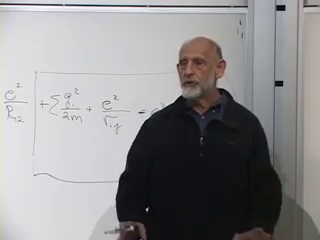
\includegraphics[width=0.72\textwidth]{lecture_01_figure_02.png}
\caption{전자 바닥 상태 문제를 소개하면서 분자의 해밀토니안을 칠판에 남겨 두었다. 이 장면에서 가려진 항들은 식 ~\eqref{eq:molecular-hamiltonian}의 조판된 형태에 나와 있다.}
\lectureframe{00:16:19}
\end{figure}

\begin{classroomqa}
\audiencequestion{원자핵의 운동량을 그냥 0으로 두는 건가요?\lecturetimestamp{00:15:39}}
\lecturerresponse{일시적으로만 그렇다. 첫 번째 근사에서는 원자핵이 전자보다 훨씬 느리게 움직이므로 못으로 고정해 둔 것처럼 취급한다. 유효 원자핵 문제를 풀 때는 운동량을 다시 포함하므로 이 근사는 불확정성 원리를 위배하지 않는다.}
\end{classroomqa}

이제 전자 바닥 상태 에너지는 원자핵이 느끼는 퍼텐셜에 기여한다.
\begin{equation}
V_{\mathrm{eff}}(R_1,R_2)
=\frac{e^2}{R_{12}}+E_{\mathrm{el}}(R_1,R_2).
\label{eq:molecular-effective-potential}
\end{equation}
두 원자만 고립된 경우 회전 및 병진 대칭성에 따라 이 퍼텐셜은 두 원자 사이 거리 \(R_{12}\)의 함수로 줄어든다. 아주 짧은 거리에서는 원자핵의 쿨롱 반발력이 지배적이다. 아주 먼 거리에서는 상호작용이 거의 없다. 그 사이에서는 전자 구름이 인력 영역과 퍼텐셜 에너지의 최솟값을 만들 수 있다. 그러면 원자핵의 파동함수는 그 최솟값 부근에 자리 잡고 결합 분자를 기술한다.

계산의 순서에 주목하자. 경험적으로 인력을 가정한 뒤 전자를 버린 것이 아니다. 먼저 고정된 원자핵 배경에서 전자의 양자 문제를 풀었다. 그런 다음에야 전자의 명시적 좌표를 지우고 그 결과로 얻은 고유값을 남겼다. 짧은 거리 물리학은 \(V_{\mathrm{eff}}\)의 모양과 깊이, 곡률에 그대로 남는다. 최솟값의 위치가 평형 거리를 정하고, 곡률이 작은 진동을 좌우하며, 점근적 형태가 결합 상태의 존재 여부를 결정한다. 하나의 유효 함수가 이 모든 전자 정보를 더 느린 문제로 전달한다.

따라서 복잡한 다전자 해밀토니안은 새로운 퍼텐셜을 갖는 두 핵의 해밀토니안이 되었다. 빠른 자유도는 제거했지만 저에너지에서의 완전한 효과는 남겼다. 퍼텐셜은 재규격화되었다. 익숙한 Born--Oppenheimer 추론은 보통 그런 이름으로 소개되지는 않지만, 우리가 필요로 하는 바로 그 생각을 담고 있다: \begin{equation}
\begin{gathered}
\text{fast microscopic dynamics}\\
\Downarrow\\
\text{effective parameters for slow dynamics}
\end{gathered}
\end{equation}

\section{자연 단위계와 장의 차원}

양자장론에서는 제거할 모드를 짧은 거리, 짧은 파장, 높은 진동수 또는 높은 에너지 모드라고 서로 바꾸어 표현할 수 있다. 그림을 그리기 전에 차원 계산의 기준부터 정하자.

일반 역학에서는 길이, 시간, 질량을 서로 독립적인 단위로 쓴다. 입자물리학에서는
\begin{equation}
\hbar=c=1.
\end{equation}
라고 둔다. 그러면 \(E=mc^2\)에 의해 에너지와 질량이 동등하고, \(c=1\)이므로 길이와 시간이 동등하며, \(\hbar=1\)에 의해 운동량은 길이의 역수가 된다. 남는 차원은 하나뿐이다.
\begin{equation}
[M]=[E]=[p]=L^{-1},
\qquad
[x]=[t]=L.
\label{eq:natural-units}
\end{equation}

차원이 사라지는 것은 아니다. 시간은 길이로, 질량은 길이의 역수로 나타내도록 환산 인자를 정하는 것이다. 한 단위만 정하면 다른 단위는 모두 따라온다. 따라서 절단 에너지는 짧은 거리 \(\delta\)로도, 높은 에너지 \(\Lambda=1/\delta\)로도 나타낼 수 있다. 두 표현은 같은 규모를 서로 다른 언어로 쓴 것이다.

하나의 실수 스칼라장 \(\phi\)를 택하고, 라그랑지언 밀도를 개략적으로 다음과 같이 정규화하자.
\begin{equation}
\mathcal L=(\partial_\mu\phi)(\partial^\mu\phi)-V(\phi),
\qquad
S=\int d^4x\,\mathcal L.
\label{eq:scalar-action}
\end{equation}

\begin{figure}[htbp]
\centering
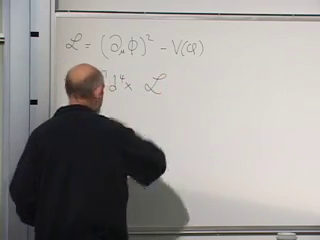
\includegraphics[width=0.78\textwidth]{lecture_01_figure_03.png}
\caption{국소 스칼라 라그랑지언 밀도와 이를 시공간에 적분해 얻는 작용.}
\lectureframe{00:26:08}
\end{figure}

라그랑지언 밀도는 국소적이며, 시공간의 한 점을 기술한다. 작용을 정지시키면 고전적인 장 방정식이 나온다. 양자론에서는 같은 작용이 경로적분의 위상 \(\exp(iS)\)에 들어간다. 어느 관점에서 보더라도 \(S\)의 차원이 중요하다. \(\hbar\)를 복원하면 위상은 \(\exp(iS/\hbar)\)이고, \(\hbar=1\)로 두면 \(S\) 자체가 무차원이어야 한다.

\begin{classroomqa}
\audiencequestion{작용의 단위는 \(\hbar\)인가요?\lecturetimestamp{00:26:13}}
\lecturerresponse{그렇다. \(\hbar\)를 1로 두었으므로 이 단위계에서 작용은 무차원이다. 4차원 측도의 차원은 \(L^4\)이므로 라그랑지언 밀도의 차원은 \(L^{-4}\)이어야 한다.}
\end{classroomqa}

이제 운동항으로 장의 차원이 정해진다.
\begin{align}
[S]&=1, & [\mathcal L]&=L^{-4},\\
[\partial_\mu]&=L^{-1}, &
[(\partial\phi)^2]&=L^{-2}[\phi]^2=L^{-4},\nonumber\\
&& [\phi]&=L^{-1}.
\label{eq:scalar-dimension}
\end{align}
이 간단한 계산으로 뒤에 나올 모든 파인만 도표의 자외선 규모를 정할 수 있다.

퍼텐셜을 다음과 같이 전개하자.
\begin{equation}
V(\phi)=\frac{m^2}{2}\phi^2+g\phi^3+\lambda\phi^4+\cdots.
\label{eq:scalar-potential}
\end{equation}
각 항의 차원은 모두 \(L^{-4}\)이어야 한다. \([\phi^n]=L^{-n}\)이므로,
\begin{equation}
[m^2]=L^{-2},
\qquad
[g]=L^{-1},
\qquad
[\lambda]=1.
\label{eq:coupling-dimensions}
\end{equation}
사차 결합 상수는 무차원이다. 이런 결합 상수는 단순한 길이 거듭제곱만으로는 척도 의존성을 알 수 없기 때문에 재규격화에서 특히 중요하다.

\begin{classroomqa}
\audiencequestion{\(g\)의 단위는 질량인가요?\lecturetimestamp{00:29:52}}
\lecturerresponse{그렇다. 인자 \(\phi^3\)의 차원은 \(L^{-3}\)이고, 퍼텐셜 밀도의 차원은 \(L^{-4}\)이어야 한다. 따라서 \([g]=L^{-1}\)이며, 자연 단위계에서는 질량의 차원이다.}
\end{classroomqa}

\section{꼭짓점과 짧은 거리 전파자}

파인만 규칙은 꼭짓점과 전파자로 이루어진다. 항 \(g\phi^3\)은 세 개의 선이 만나는 꼭짓점을 주며, 여기에 비례하는 인자는 \(g\)이다. 항 \(\lambda\phi^4\)은 네 개의 선이 만나는 꼭짓점을 주며, 여기에 비례하는 인자는 \(\lambda\)이다. 이차항은 국소적인 2점 삽입을 준다. 입자가 들어와 흡수된 뒤 다시 방출되는 것으로 그릴 수 있으며, 계수는 \(m^2/2\)에 비례한다. 강의에서는 단면을 계산하는 대신 척도 의존성을 추출하므로 수치 정규화, 부호, \(i\) 인자와 대칭 인자를 일부러 생략한다.

이 그림들은 실제 과정으로 해석할 수 있다. 3점 꼭짓점은 양자 두 개를 흡수하고 하나를 방출하는 과정일 수도 있고, 세 선을 교차 대칭에 따라 다르게 배정한 과정일 수도 있다. 4점 꼭짓점은 입자 두 개가 들어와 두 개가 나가는 과정을 기술할 수 있다. 이차 교차 표시는 보통 자유 전파자에 포함되지만, 여전히 가능한 2선 꼭짓점이다. 잠시 후 분해되지 않은 모든 2점 과정은 이것과 비교해 알아볼 수 있으므로 여기서 표시해 둔다.

전파자는 시공간의 두 점을 연결한다. 전파자 선은 양자 입자가 고전적인 직선 경로를 따라 움직였다는 뜻이 아니다. 이는 \(x\)에서 장 여기 상태를 만들고 \(y\)에서 제거하거나 검출할 진폭을 나타낸다.
\begin{equation}
\Delta(x-y)=\langle0|\phi(y)\phi(x)|0\rangle.
\label{eq:position-propagator}
\end{equation}
식을 오른쪽에서부터 읽어 보자. 진공에 \(\phi(x)\)를 작용시키면 \(x\)에 한 입자 성분이 생성된다. 브라에 \(\phi(y)\)를 작용시키면 \(y\)에서 그 성분이 제거된다. 두 작용의 진공 행렬원소는 첫 번째 점에서 생성된 상태와 두 번째 점에서 검출된 상태 사이의 중첩 진폭이다. 기호 \(x\)와 \(y\)는 두 개의 카르테시안 좌표만이 아니라 4차원 벡터 전체를 가리킨다.

상태에는 물리적 차원이 없고 장마다 \(L^{-1}\)가 기여한다. 따라서
\begin{equation}
[\Delta]=L^{-2}.
\end{equation}
질량 없는 장에는 고유한 길이 척도가 없으므로 차원 분석에 따라 짧은 거리에서의 거동은 다음과 같다.
\begin{equation}
\Delta(x-y)\sim\frac{1}{(x-y)^2}.
\label{eq:massless-propagator}
\end{equation}
분모는 로런츠 불변인 거리 제곱이며, 특이점에서는 통상적인 처방이 필요하다.\editorialnote{승수 계산에는 유클리드 거리로 위크 회전하면 편리하다. 이때 크기는 모호함 없이 \(1/|x-y|^2\)에 비례한다. 이 변환은 아래에서 사용하는 자외선 거듭제곱을 바꾸지 않는다.}

\(y\)가 \(x\)에 가까워지면 전파자는 발산한다. 분리 거리가 사라질 때 나타나는 전파의 특이성이 더 복잡한 도표에서 자외선 발산이 생겨나는 근원이다.

\section{스칼라 질량의 재규격화}

스칼라장의 동역학적 매개변수는 \(m^2\)이다. 이는 상대론적 분산 관계만 보아도 알 수 있다.
\begin{equation}
E=\sqrt{\mathbf p^2+m^2}.
\end{equation}
유효 기술이 분해하는 가장 짧은 거리를 \(\delta\)라 하자. 꼭짓점 사이 거리가 \(\delta\)보다 짧은 과정은 구별하지 않기로 한다. 들어오는 스칼라 하나와 나가는 스칼라 하나가 있는, 분해되지 않은 과정은 관측 가능한 형태가 질량 삽입과 같으므로 유효 질량에 기여해야 한다.

가속기를 현미경이라고 생각해 보자. 가장 정밀한 분해능이 \(\delta\)라면, 한 점에서 입자가 흡수된 다음 \(\delta\)보다 훨씬 짧은 거리 뒤에서 방출되는 과정은 진정한 국소 사건과 구별할 수 없다. 그 길이 규모의 꼭짓점들을 의도적으로 흐릿하게 본다. 재규격화란 분해능 아래의 모든 대안을 해당 국소 연산자의 계수에 반영하는 규칙이다.

\subsection{첫 번째 사차 보정}

\(\phi^4\) 꼭짓점 하나에서 시작하자. 두 다리는 외부 입자이고, 나머지 두 다리는 거의 같은 지점에서 방출되었다가 재흡수되는 짧은 고리를 이룬다. 일치하는 점의 전파자를 절단 거리만큼 퍼뜨리면
\begin{equation}
\Delta(0)\ \longrightarrow\ \Delta(\delta)\sim\frac{1}{\delta^2},
\end{equation}
따라서
\begin{equation}
\delta m^2_{(1)}\sim\frac{\lambda}{\delta^2}.
\label{eq:one-loop-scalar-mass}
\end{equation}
\(m_0^2\)가 입력값 또는 맨 처음의 매개변수라면, 낮은 분해능에서의 2점 계수는 개략적으로 다음과 같다.
\begin{equation}
\frac{m_{\mathrm{eff}}^2}{2}
\sim
\frac{m_0^2}{2}
+c_1\frac{\lambda}{\delta^2},
\label{eq:first-renormalized-mass}
\end{equation}
여기서 \(c_1\)에는 무시한 수치 인자와 관례에 따라 달라지는 인자가 들어 있다. \(\delta\)보다 짧은 거리를 분해하지 못하는 실험에서 측정하는 실험실 질량은 \(m_0\) 자체가 아니라 이렇게 재규격화된 양이다.

따라서 관측된 2점 사건이 일어나는 방식은 서로 구별할 수 없는 두 가지다. 원래의 이차 꼭짓점에서 입자가 흡수되었다가 재방출될 수도 있고, 사차 상호작용에서 가상 스칼라를 잠시 방출했다가 재흡수하는 방식으로 같은 일이 일어날 수도 있다. 양자역학에서는 진폭을 더한다. 고리가 분해능보다 작은 영역에 놓이면 그 개별 과정은 유효 기술에서 사라지지만, 측정되는 계수에 대한 기여는 남는다.

\subsection{다음 사차 보정}

이번에는 사차 꼭짓점 두 개를 연결하자. 외부 입자 하나가 \(x\)에서 들어오고 하나가 \(x+\Delta\)에서 나가며, 세 개의 내부 전파자가 두 꼭짓점을 잇는다. \(\lambda\)은 두 번 곱해지고, 전파자들은 \(\Delta^{-6}\)를 준다. 양자 진폭은 나가는 입자가 나타날 수 있는 분해되지 않은 모든 위치에 대해 더해야 하므로, 상대 4차원 벡터를 적분한다.
\begin{equation}
\delta m^2_{(2)}
\sim
\lambda^2
\int_{|\Delta|\gtrsim\delta}
d^4\Delta\,\frac{1}{|\Delta|^6}.
\label{eq:two-loop-power-count}
\end{equation}

\begin{classroomqa}
\audiencequestion{꼭짓점의 작은 표시를 보면 입자가 세 개만 있다는 뜻인가요?\lecturetimestamp{00:46:35}}
\lecturerresponse{아니다. 여전히 사차 상호작용을 사용한다. 각 꼭짓점에는 네 개의 선이 만나며, 이 2점 도표에서는 한 선이 외부선이고 세 선이 두 꼭짓점 사이를 지난다. 두 번째 꼭짓점에도 네 개의 선이 들어온다.}
\end{classroomqa}

측도는 길이의 4제곱을 주고 세 전파자는 길이의 -6제곱을 준다. 이 계산에서 유일한 척도는 자외선 절단이므로,
\begin{equation}
\int_{|\Delta|\gtrsim\delta}
\frac{d^4\Delta}{|\Delta|^6}
\sim\frac{1}{\delta^2},
\qquad
\delta m^2_{(2)}
\sim\frac{\lambda^2}{\delta^2}.
\label{eq:two-loop-scalar-mass}
\end{equation}
여기서 \(\Delta^\mu\)는 네 성분을 가진 적분 변수다. 시간 성분과 공간 성분 세 개에 대해 적분한다. 소문자 \(\delta\)는 고정된 절단 길이다. 강의에서는 처음에 두 기호를 같은 이름으로 부르다가 뒤에 표기를 바로잡는다.

4차원 측도를 반지름 방향으로 적으면 같은 결과를 확인할 수 있다. 각도에 따른 상수 인자를 제외하면
\begin{equation}
\int_{\delta}\frac{d^4\Delta}{|\Delta|^6}
\sim
\int_{\delta}\frac{R^3\,dR}{R^6}
=\int_{\delta}\frac{dR}{R^3}
\sim\frac{1}{\delta^2}.
\end{equation}
이것이 자외선 추정에서 큰 거리 쪽 적분 상한이 중요하지 않은 이유다. 적분값은 하한에서 주로 결정된다.

더 높은 차수의 도표에서도 같은 양상이 반복된다. 사차 꼭짓점이 더 많은 도표에서는 \(\lambda\)의 거듭제곱이 더 높아지지만, 차원 분석에 따르면 여전히 질량에 이차 발산 기여가 가능하다.
\begin{equation}
\begin{aligned}
m_{\mathrm{eff}}^2
={}&m_0^2
+\frac{1}{\delta^2}
\left(c_1\lambda+c_2\lambda^2+c_3\lambda^3+\cdots\right)\\
&+\text{weaker terms}.
\end{aligned}
\label{eq:scalar-mass-series}
\end{equation}

\subsection{삼차 상호작용과 로그}

삼차 꼭짓점 두 개 사이에는 가까운 두 점을 잇는 전파자 두 개가 있다. 이들의 기여는 다음과 같이 스케일링한다.
\begin{equation}
\delta m_g^2
\sim
g^2\int_{|\Delta|\gtrsim\delta}
\frac{d^4\Delta}{|\Delta|^4}.
\label{eq:cubic-loop}
\end{equation}
이제 측도와 분모의 거듭제곱이 같다. 남는 의존성은 거듭제곱이 아니라 로그다.
\begin{equation}
\delta m_g^2
\sim
c_g g^2\log\!\left(\frac{1}{\mu\delta}\right).
\label{eq:cubic-log}
\end{equation}
기준 척도 \(\mu\)를 넣으면 로그의 인자가 무차원이 된다. 이것이 강의의 개략적인 \(g^2\log\delta\)을 차원을 갖춘 형태로 나타낸 것이다. 로그는 역수 거듭제곱보다 훨씬 느리게 변하므로 절단 길이가 짧아질수록 \(1/\delta^2\)이 지배적이다.

이번에도 반지름 방향으로 쓰면 차이가 분명해진다.
\begin{equation}
\int_{\delta}^{R_{\mathrm{IR}}}
\frac{d^4\Delta}{|\Delta|^4}
\sim
\int_{\delta}^{R_{\mathrm{IR}}}\frac{R^3\,dR}{R^4}
=\log\!\left(\frac{R_{\mathrm{IR}}}{\delta}\right).
\end{equation}
측도와 분모의 거듭제곱이 같으면 로그가 생긴다. 분모의 거듭제곱이 더 크면 절단 길이의 역수 거듭제곱이 생긴다. 강의의 목적은 각도 인자를 계산하는 것이 아니라, 자외선에서의 답을 한눈에 알아보는 것이다.

\begin{classroomqa}
\audiencequestion{로그의 밑은 무엇인가요?\lecturetimestamp{00:57:42}}
\lecturerresponse{자연로그를 쓴다. 밑을 바꾸면 로그에 수치 상수만 곱해지며, 그 상수는 여기서 계산하지 않은 \(2\), \(\pi\), 대칭 인자들을 포함하는 계수에 흡수된다.}
\end{classroomqa}

\begin{classroomqa}
\audiencequestion{길이의 로그를 어떻게 취할 수 있나요? 질량 보정항의 단위는 어디서 나오나요?\lecturetimestamp{00:58:32}}
\lecturerresponse{로그는 언제나 두 척도를 비교한다. 따라서 실제로는 \(1/(\mu\delta)\) 같은 무차원 비의 로그를 취하는 것이다. 결합 상수 \(g\)는 질량의 차원을 한 번 가지므로, \(g^2\)는 보정항에 필요한 질량 제곱 차원을 이미 정확히 갖는다.}
\end{classroomqa}

\begin{classroomqa}
\audiencequestion{파인만 도표는 진폭을 준다고 하셨는데, 그 절댓값의 제곱이 확률인가요?\lecturetimestamp{00:59:41}}
\lecturerresponse{필요한 상태 인자와 위상 공간 인자를 포함해 물리적 전이 계산에 넣으면 그렇다. 여기서 진폭의 더 직접적인 역할은 다르다. 분해되지 않은 2점 진폭은 질량항과 같은 국소 형태이므로 유효 질량 매개변수를 이동시킨다.}
\end{classroomqa}

\section{모든 매개변수는 유효량이 된다}

질량 도표가 무한히 많다는 사실은 \(\lambda\)가 작다고 해서 사라지지 않는다. 섭동론에서는 이들을 결합 상수의 거듭제곱에 따라 순서 짓기 때문에 연속되는 항이 차례로 작아질 수 있지만, 항의 수는 여전히 무한하다. 같은 짧은 거리 자유도 제거 과정은 상호작용 자체도 재규격화한다.

\begin{classroomqa}
\audiencequestion{질량 재규격화에도 도표가 무한히 많지 않나요?\lecturetimestamp{01:00:35}}
\lecturerresponse{그렇다. \(\lambda\)가 충분히 작으면 더 높은 거듭제곱의 항이 차례로 억제되므로 섭동 급수가 유용할 수 있다. 그래도 재규격화된 매개변수는 첫 번째 그림 하나가 아니라 급수 전체로 정의된다.}
\end{classroomqa}

실제로 국소적인 \(\lambda\phi^4\) 상호작용은 입자 두 개가 들어오고 두 개가 나가는 진폭이다. 더 복잡한 4점 과정이 분해되지 않은 영역 안에서 모두 일어나면 낮은 분해능에서는 원래의 국소 꼭짓점과 구별할 수 없다. 따라서 그런 도표의 기여를 유효한 \(\lambda\)에 합쳐 넣는다. 4차원 \(\phi^4\) 이론에서 그 주된 척도 의존성은 보통 로그 형태다. 강의에서는 베타 함수를 계산하지 않고 이 사례로 일반적인 점을 설명한다.
\begin{equation}
\begin{gathered}
\text{parameters measured at low energy}\\
\ne\\
\text{parameters entered at the microscopic cutoff}
\end{gathered}
\end{equation}

4점 사례가 중요한 이유는 재규격화가 질량 발산에만 적용하는 특별한 보수 작업이라는 오해를 없애기 때문이다. 라그랑지언에서 허용되는 모든 연산자는 같은 외부선을 갖고 같은 대칭성을 따르는 분해되지 않은 도표로 재현될 수 있다. 2점 과정은 이차 계수를, 4점 과정은 사차 계수를 재규격화하며, 진공에서 진공으로 가는 과정은 상수항을 재규격화한다. 저에너지 라그랑지언은 이런 짧은 거리 과정 모두를 기록하는 간결한 장부다.

\begin{classroomqa}
\audiencequestion{\(\Delta\)의 단위가 길이라면 그 로그는 차원상 이상하지 않나요? 칠판에서는 대문자 델타와 소문자 델타를 바꿔 쓴 건가요?\lecturetimestamp{01:01:34}}
\lecturerresponse{로그는 실제로 다른 척도에 대한 비를 뜻하므로 무차원이다. 맞다. 표기를 잠시 뒤바꾸어 썼다. \(\Delta^\mu\)는 적분 변수이고, \(\delta\)는 최종 답에 남는 하한 거리 절단이다.}
\end{classroomqa}

이것은 분자 사례에 대응하는 장론의 설명이다. 보이지 않는 빠른 전자를 풀고 그 결과를 퍼텐셜에 넣었다. 여기서는 보이지 않는 짧은 거리 과정을 모두 더하고 그 결과를 질량과 결합 상수, 그리고 허용되는 모든 국소 계수에 넣는다. 모든 항이 이동한다.

\begin{classroomqa}
\audiencequestion{실험에서 볼 수 없는 척도보다 짧은 척도까지 측정된 양에 포함되는지 다시 말씀해 주시겠어요?\lecturetimestamp{01:05:13}}
\lecturerresponse{그렇다. 개별 요동은 분해되지 않지만, 그 효과를 모두 더한 결과는 포함된다. 더 짧은 척도와 관련된 모든 도표의 기여를 하나의 유효 계수에 모으며, 저에너지 실험에서는 이를 예컨대 물리적 질량 제곱이라고 부른다.}
\end{classroomqa}

\begin{classroomqa}
\audiencequestion{그렇다면 입력항 \(m_0^2\)이 나머지 기여를 상쇄해야 하나요?\lecturetimestamp{01:06:00}}
\lecturerresponse{측정된 스칼라 질량이 개별 자외선 기여보다 훨씬 작다면 그렇다. 필요한 상쇄가 바로 이제 살펴볼 미세 조정 문제다.}
\end{classroomqa}

\section{힉스 계층성 문제}

절단 길이가 플랑크 길이라고 가정하자. 그러면 유효장론은 실험실 규모에서 양자 중력이 개입해야 하는 규모까지의 요동을 모두 요약해야 한다. 입자물리학 단위로는
\begin{equation}
\delta\sim M_{\mathrm{Pl}}^{-1}\sim10^{-19}\,\mathrm{GeV}^{-1},
\qquad
\frac{1}{\delta^2}\sim10^{38}\,\mathrm{GeV}^2.
\label{eq:planck-cutoff}
\end{equation}
환산 플랑크 척도를 쓰든 환산하지 않은 플랑크 척도를 쓰든, 엄청난 차이를 비교한다는 점은 달라지지 않는다.

플랑크 길이는 양성자 반지름보다 약 열아홉 자릿수 작고, 논의 중인 가속기들이 직접 탐사하는 거리보다 대략 열여섯에서 열일곱 자릿수 작다. 이 길이 차이를 제곱하면 길이의 큰 계층 구조가 스칼라 질량제곱 매개변수에서 대략 서른네 자릿수 규모의 상쇄로 이어진다.

스칼라인 힉스장의 바람직한 약한 상호작용 척도는 수백 GeV 정도이지, \(10^{19}\) GeV가 아니다. 그런데 식 ~\eqref{eq:scalar-mass-series}의 항들은 자연스럽게 플랑크 척도 크기가 될 수 있다. 각 항의 부호는 따져 보지 않았다. 양수인 항도 음수인 항도 있을 수 있고, 맨 처음의 질량 제곱도 어느 부호든 가질 수 있다. 그러나 전기약 척도의 나머지 값을 남기려면 이처럼 거대한 항들이 대략 소수점 아래 34자리까지 상쇄되어야 한다. 서스킨드는 처음에 17자리라고 했다가 비교 대상이 질량의 제곱임을 감안해 바로잡는다. 이 조정의 정도를 나타내는 것은 제곱한 비다.

\begin{classroomqa}
\audiencequestion{\(\lambda\)는 1보다 작습니까, 큽니까?\lecturetimestamp{01:09:50}}
\lecturerresponse{1보다 약간 작은 값으로 가정합니다. 연속되는 차수의 항이 커진다면 섭동 이론은 다루기 어려워지고, 순수 스칼라 이론도 사중 결합이 임의로 커지는 경우 일관되게 외삽할 수 없습니다. 하지만 \(\lambda\)는 \(10^{-38}\)만큼 작지는 않습니다. 이 강의에서는 감을 잡기 위해 퍼센트 규모의 값을 사용합니다.}
\end{classroomqa}

\begin{classroomqa}
\audiencequestion{\(\lambda<1\)라고 해도, 각 항에 큰 컷오프 인자가 곱해지므로 중요한 항이 많이 남지 않습니까?\lecturetimestamp{01:10:43}}
\lecturerresponse{그렇습니다. 고차 항들은 결국 급수를 억제하지만, 그렇게 되기 전까지 많은 항이 기여할 수 있습니다. 그 항들과 맨 처음 항이 모두 서로 맞물려 상쇄되어야만 물리적으로 관측되는 값이 그토록 작아집니다.}
\end{classroomqa}

힉스 질량 매개변수가 약한 규모라는 사실을 어떻게 아는지 되짚어 봅시다. 이 강의의 표기법에 따라 대칭 깨짐 퍼텐셜을 다음과 같이 씁니다.
\begin{equation}
V(\phi)=-\frac{\mu^2}{2}\phi^2+\frac{\lambda}{4}\phi^4.
\label{eq:higgs-potential}
\end{equation}
음의 이차항 계수 때문에 원점은 불안정하고, 양의 사차항은 퍼텐셜을 안정화합니다. 미분하면
\begin{equation}
\frac{dV}{d\phi}=-\mu^2\phi+\lambda\phi^3
=\phi(-\mu^2+\lambda\phi^2),
\end{equation}
영이 아닌 극솟값을 얻습니다.
\begin{equation}
\phi_{\min}^2=f^2=\frac{\mu^2}{\lambda}.
\label{eq:higgs-minimum}
\end{equation}
판서에서는 사차항을 \(\lambda\phi^4\)처럼 개략적으로 쓰지만, ~\eqref{eq:higgs-minimum}을 인용합니다. 관례적인 인자 \(1/4\)를 넣으면 논지를 바꾸지 않고도 두 식이 서로 일치합니다.

\(-\mu^2\)의 부호는 중요하지만 자연성 문제를 해결해 주지는 않습니다. 자발적 대칭 깨짐을 일으키는 것은 원점에서의 음의 곡률입니다. 재규격화는 그 곡률을 큰 양의 항과 음의 항만큼 이동시킵니다. 관측된 깨진 진공을 얻으려면 두 항의 합이 단지 작기만 해서는 안 됩니다. 극솟값이 약한 규모에 놓이도록 특정한 작은 음수여야 합니다.

\(W\) 보손과 \(Z\) 보손의 질량으로부터, 이 강의에서 사용하는 대략적인 정규화에서는 \(f\)가 \(200\,\mathrm{GeV}\) 규모임을 알 수 있습니다. \(\lambda\)가 엄청나게 크지도 터무니없이 작지도 않다면, \(\mu\)도 대체로 비슷한 규모여야 합니다. 따라서 관측된 약한 규모의 계수는 각각 수십 자릿수 더 클 수도 있는 기여들의 잔여분입니다.

이를 힉스 미세 조정 문제, 계층 문제 또는 게이지 계층 문제라고 합니다. 여기서 계층이란 보통의 약한 규모와 가능한 대통일 규모 또는 플랑크 규모 사이의 엄청난 비율을 뜻합니다. 작은 수라는 사실만으로 반드시 역설이 되는 것은 아닙니다. 여기서 문제를 일으키는 것은 크고 서로 무관해 보이는 항들을 극도로 정밀하게 상쇄해 만들어 낸 작은 수입니다. 이 문제는 1970년대 후반과 1980년대 초반에 인식되었으며, 그 상쇄의 배후에 있는 메커니즘을 찾으려는 노력이 초대칭과 여러 경쟁 이론의 동기가 됩니다.

무한한 섭동 급수는 이 수수께끼를 없애기보다 더 두드러지게 합니다. 퍼센트 규모의 \(\lambda\)라면 충분히 고차인 거듭제곱은 작아지지만, 억제가 우세해지기 전에 많은 항이 나타날 수 있습니다. 한 루프가 우연히 맨 처음 질량을 상쇄하는 것만으로는 충분하지 않습니다. 나머지 단거리 과정까지 포함한 뒤에도 유효한 약한 규모가 안정적으로 유지되어야 합니다. 항들 사이의 구조적 관계가 있다면 설명이 되겠지만, 서로 무관한 숫자들을 자릿수마다 맞춰 상쇄하는 것은 미세 조정일 뿐입니다.

\section{페르미온 질량은 왜 더 잘 다루어지는가}

표준 모형의 다른 입자들은 같은 종류의 독립적인 미세 조정을 필요로 하지 않습니다. 디랙 페르미온의 질량항은 다음과 같습니다.
\begin{equation}
\mathcal L_m=-m\bar\psi\psi
=-m\left(\bar\psi_L\psi_R+\bar\psi_R\psi_L\right).
\label{eq:fermion-mass}
\end{equation}
여기에는 질량의 제곱이 아니라 질량이 들어가며, 왼손성과 오른손성을 결합합니다. 따라서 국소적인 질량 삽입은 \(L\)를 \(R\)로, 또는 \(R\)을 \(L\)로 바꿉니다.

\begin{figure}[htbp]
\centering
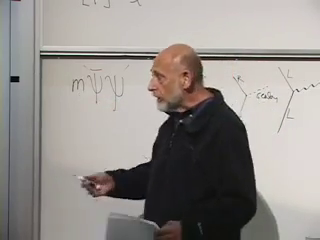
\includegraphics[width=0.76\textwidth]{lecture_01_figure_04.png}
\caption{페르미온 질량항과 손지기성을 바꾸는 선 도식. 분필로 그린 내용 일부가 가려져 있어, 아래에서는 대수적으로 도식을 재구성합니다.}
\lectureframe{01:23:36}
\end{figure}

강의 중에는 흔히 손잡이성 또는 헬리시티라는 말을 씁니다. 정확한 보호를 가장 명확히 나타내려면 손지기성으로 설명하는 것이 좋습니다. 초상대론적 입자의 경우 헬리시티 그림이 의도한 직관을 제공하지만, ~\eqref{eq:fermion-mass}에서 왼손 및 오른손 장이 지니는 양은 손지기성입니다.

게이지 상호작용은 손지기성을 보존합니다.
\begin{equation}
L\xrightarrow{\ \gamma\ }L,
\qquad
R\xrightarrow{\ \gamma\ }R.
\label{eq:gauge-preserves-chirality}
\end{equation}
스칼라와의 유카와 상호작용은 반대 손지기성을 연결합니다.
\begin{equation}
L\xleftrightarrow{\ \phi\ }R.
\label{eq:scalar-flips-chirality}
\end{equation}
먼저 전자가 \(m_0=0\)에서 시작한다고 합시다. 광자를 몇 개나 방출하고 재흡수하더라도 질량이 생길 수는 없습니다. 모든 게이지 꼭짓점이 손지기성을 보존하기 때문입니다. 왼쪽에서 시작한 상태는 계속 왼쪽으로 남습니다. 따라서 순수 양자전기역학에서는 질량이 없는 전자를 일관되게 허용합니다. 전자기 자기 에너지는 질량이 0인 상태에서 가산적인 질량을 만들어 낼 수 없습니다.

선 도식으로 보면 왼손 손지기 전자에서 시작합니다. 첫 번째 광자 꼭짓점에서도 왼손 손지기 상태이며, 전파된 뒤 광자를 재흡수하고 나서도 여전히 왼손 손지기 상태입니다. 이 과정을 반복하면 손지기성을 보존하는 꼭짓점만 더 삽입됩니다. 외부 두 점 함수는 재규격화될 수 있지만, 질량을 정의하는 왼손과 오른손의 구조를 얻을 수는 없습니다.

스칼라 방출은 어떨까요? 스칼라 꼭짓점 하나는 \(L\)를 \(R\)로 바꾸지만, 방출된 스칼라는 다시 흡수되어야 합니다. 따라서 두 점 자기 에너지 도식에는 스칼라 꼭짓점이 짝수 개 들어갑니다. 두 번째 뒤집힘은 첫 번째를 되돌리므로, 전체 도식은 다시 외부 손지기성을 보존합니다. 내부 도식이 아무리 복잡해져도 스칼라의 방출과 재흡수는 꼭짓점들을 짝지어, 처음 질량이 0일 때 가산적인 \(L\)에서 \(R\)로의 항이 나타나지 못하게 합니다.

이는 뒤집힘 횟수의 홀짝성에 관한 논증입니다. 스칼라 꼭짓점 하나는 손지기성을 한 번 뒤집습니다. 내부 스칼라 선을 모두 닫으려면 두 번째 끝점, 곧 두 번째 뒤집힘이 필요합니다. 스칼라 꼭짓점이 네 개면 네 번 뒤집히는 식입니다. 짝수 번 뒤집히면 페르미온은 원래 손지기성으로 돌아옵니다. 이 결론은 판서에 그린 가장 단순한 루프에만 국한되지 않습니다.

도식에 질량 삽입이 이미 포함되어 있어야 비영 질량 보정이 가능해집니다. 예를 들어, 광자의 방출과 재흡수 사이에 \(m_0\bar\psi\psi\) 삽입 하나가 놓일 수 있습니다. 게이지 꼭짓점은 전하의 제곱에 해당하는 인자를 두 개 제공하지만, 손지기성을 뒤집는 유일한 과정은 처음 질량을 제공합니다.
\begin{equation}
\begin{aligned}
m_e
&=m_0+c_1e^2m_0+c_2e^4m_0+\cdots\\
&=m_0\left(1+c_1e^2+c_2e^4+\cdots\right).
\end{aligned}
\label{eq:multiplicative-fermion-mass}
\end{equation}
\(m_0=0\)이면 결과는 계속 0입니다. \(m_0\)가 작으면 모든 보정이 그 작은 값에 비례합니다. 전자가 근본적인 규모에 비해 왜 가벼운지는 여전히 물을 수 있지만, 그 질량을 얻기 위해 서로 무관한 거대한 수들을 빼고 있지는 않습니다. 이런 의미에서 작은 페르미온 질량은 기술적으로 자연스럽습니다.

질량 삽입으로 허용되는 순서가 명확해진다. \(L\)에서 시작하자. 광자 방출은 \(L\)을 보존하고, 삽입된 \(m_0\)는 \(L\)을 \(R\)로 바꾼다. 광자의 재흡수는 \(R\)를 보존한다. 이제 이 다이어그램은 질량항과 같은 외부 키랄리티를 갖지만, 그 값에는 반드시 \(m_0\) 인자가 포함된다. 이것이 ~\eqref{eq:one-loop-scalar-mass}과 결정적으로 다른 점이다. 그 식의 스칼라 보정은 처음의 스칼라 질량을 영으로 두더라도 0이 되지 않는다.

게이지 보손에도 비슷한 보호가 있습니다. 게이지 대칭은 독립적인 질량항을 금지하므로, 질량이 없는 상태에서 시작한 게이지 보손은 모든 섭동 차수에서 질량이 없습니다. 표준 모형에서는 힉스 기대값에 따라 페르미온과 약한 게이지 보손의 질량이 생깁니다. 힉스 규모를 제어하면, 나머지 가벼운 질량에 같은 파국적 미세 조정을 각각 별도로 적용할 필요가 없습니다.

이로써 초대칭이 다루려는 문제가 드러납니다. 이론이 힉스 스칼라에 거대한 가산적 질량 보정이 생기는 것을 막을 수 있을까요? 적절한 초대칭 이론에서는 그렇습니다. 보손 기여와 페르미온 기여가 서로 독립적이지 않고 관계를 맺기 때문입니다. 구체적인 메커니즘은 다음 강의에서 다룹니다.

\section{또 다른 미세 조정 문제: 진공 에너지}

훨씬 더 심각한 재규격화 문제가 하나 있지만, 중력이 포함되어야 관측할 수 있습니다. 중력이 없는 물리에서는 모든 에너지에 상수를 더해도 어떤 실험 결과도 달라지지 않습니다. 예를 들어 전자 질량은 절대적인 에너지가 아닙니다. 진공에 전자 하나를 더하는 데 필요한 추가 에너지입니다.
\begin{equation}
m_e=E(\text{vacuum}+\text{one electron})-E(\text{vacuum})
\end{equation}
이는 전자의 정지 계에서 그렇습니다. 진공과 모든 들뜬 상태가 함께 이동한다면, 그 차이는 변하지 않습니다.

그럼에도 진공에서 진공으로 이어지는 도식은 진공 에너지를 이동시킵니다. \(\lambda\phi^4\) 이론에서는 사차 꼭짓점 하나의 네 다리를 두 개의 짧은 루프로 연결할 수 있습니다. 한 점에서의 전파인자마다 \(1/\delta^2\)가 주어지므로,
\begin{equation}
\delta\rho_{\mathrm{vac}}
\sim
c_{\mathrm{vac}}\frac{\lambda}{\delta^4}.
\label{eq:vacuum-energy-divergence}
\end{equation}
더 복잡한 진공 도식에는 서로 다른 결합상수와 계수가 들어가지만, 차원 분석을 하면 에너지 밀도는 대체로 같은 사차 컷오프 민감도를 갖습니다.

외부 선이 없다는 점이 바로 이 보정을 식별하는 특징입니다. 두 점 도식은 한 입자 상태와 진공을 비교해 질량을 바꾸고, 네 점 도식은 산란을 바꾸며, 들어오거나 나가는 입자가 없는 도식은 진공에서 진공으로의 진폭 자체를 바꿉니다. 사차 꼭짓점 하나가 \(\lambda\)를 제공하고, 짧은 루프 두 개가 각각 \(\delta^{-2}\)를 제공합니다. 따라서 차원 분석에 따르면 에너지 밀도 규모는 \(\delta^{-4}\)여야 합니다.

중력이 없다면 에너지의 가산 상수를 선택해도 되므로 누가 신경 쓰겠느냐고 물을 수 있습니다. 일반 상대성 이론에서는 그 자유가 사라집니다. 에너지-운동량이 시공간 곡률의 원천이므로, 균일한 진공 에너지도 빈 공간을 중력에 반응하게 만듭니다. 진공 에너지는 우주 상수로 나타나며 관측상 암흑 에너지와 연결됩니다. 따라서 측정된 진공 에너지가 작으려면 \(\delta^{-4}\) 형태의 기여들을 상쇄한 뒤에도 그 값이 작게 남아야 합니다.

중력을 켜면 질문이 달라지는 이유가 여기에 있습니다. 보통의 양자역학에서는 모든 에너지 준위를 같은 상수만큼 이동해도 전이 진동수는 바뀌지 않습니다. 중력에서는 그 상수가 아무런 영향을 주지 않는 항이 아닙니다. 진공 응력 텐서는 계량 텐서에 비례해 시공간을 휘게 합니다. 임의로 정할 수 있었던 에너지의 영점이 아인슈타인 방정식의 원천이 됩니다.

따라서 자연성에 관한 심각한 수수께끼는 적어도 두 가지입니다. 강의에서는 진공 에너지 미세 조정에 대략 123자리, 힉스 질량 미세 조정에 대략 30--35자리가 필요하다고 합니다. 정확한 자릿수는 자외선 규모와 관례에 따라 달라지지만, 둘 사이의 차이는 분명합니다. 초대칭은 여기서 논의한 힉스 문제에 대한 가능한 대응입니다. 초대칭이 깨지고 나면, 그것만으로 관측된 우주 상수를 설명하지는 못합니다.\editorialnote{이것은 보손--페르미온의 정확한 초대칭 상쇄가 관측된 진공 에너지에 대한 현상론적 해법이 될 수 없는 이유이기도 합니다. 우리 세계에서는 초대칭이 깨져야 합니다.}

\section{강의 마무리 질의응답}

\begin{classroomqa}
\audiencequestion{\(\delta\)에 따라 힉스 보정이 달라지지만, 컷오프는 임의적으로 보입니다. 플랑크 길이일 수도 있고, 플랑크 길이의 열 배일 수도 있고, 다른 값일 수도 있지 않습니까? 그렇다면 미세 조정도 임의적인 것 아닙니까?\lecturetimestamp{01:33:50}}
\lecturerresponse{수치상의 기여는 유효 이론을 신뢰할 수 있는 최단 규모에 따라 달라집니다. 이런 의존성은 물리적 장부 정리이지, 문제를 피하는 방법이 아닙니다. 표준 모형이 여전히 유효한 모든 규모까지의 모드는 그 효과를 포함해야 하는 모드입니다. 새 물리가 나타날 것으로 예상되는 거리, 즉 \(\delta\)를 선택합니다---. 그 규모는 플랑크 규모일 수도 있고, \(10^{16}\,\mathrm{GeV}\) 부근의 대통일 규모일 수도 있습니다. 그 규모까지 누적되는 기여만으로도 이미 문제의 하한에 해당합니다. 같은 이론을 더 짧은 거리까지 확장하면 이차 민감도는 더 커질 뿐입니다. 실험실 규모와 그 자외선 경계 사이의 모든 규모에서 오는 기여를 무엇이 상쇄하는지 설명해야 합니다.}
\end{classroomqa}

\begin{classroomqa}
\audiencequestion{스칼라 입자는 무엇으로 정의하며, 그 예에는 무엇이 있습니까?\lecturetimestamp{01:37:26}}
\lecturerresponse{여기서 들고자 하는 예는 힉스입니다. 스칼라는 공간 회전 아래서 서로 다른 성분으로 변환되지 않습니다. 다시 말해 그 입자 양자의 스핀은 0입니다. 광자는 벡터장으로, 중력장은 텐서로 기술합니다. 이 2010 강의 당시에는 기본 스핀 0 입자가 아직 검출되지 않았습니다.\editorialnote{힉스 보손은 CERN에서 2012년에 발견되었으며, 측정된 성질은 스핀 0과 일치합니다.}}
\end{classroomqa}

\begin{classroomqa}
\audiencequestion{\(Z\) 입자도 게이지 보손입니까?\lecturetimestamp{01:38:31}}
\lecturerresponse{그렇습니다. \(Z\), \(W^+\), \(W^-\)은 광자와 마찬가지로 스핀 1인 게이지 보손입니다. 이들의 장 방정식과 상호작용은 맥스웰 이론과 유사한 게이지 기술을 비가환 이론이나 전약 이론으로 일반화한 것입니다.}
\end{classroomqa}

\begin{classroomqa}
\audiencequestion{진공 에너지에서 보손 바닥 상태의 기여는 왜 페르미온의 기여와 상쇄되지 않습니까?\lecturetimestamp{01:39:10}}
\lecturerresponse{페르미온 루프와 그에 대응하는 보손 루프는 실제로 서로 반대 부호로 기여할 수 있습니다. 하지만 상쇄가 저절로 일어나는 것은 아닙니다. 입자의 질량과 중복도, 결합상수가 서로 맞아야 합니다. 작은 불일치만 있어도 컷오프에 민감한 큰 잔여분이 남고, 무한히 많은 도식들의 기여가 차수마다 맞아야 합니다. 정확한 초대칭은 바로 이런 보손--페르미온 관계를 보장합니다. 일반적인 비초대칭 입자 구성에서는 그렇지 않으며, 깨진 초대칭도 진공 에너지 문제의 잔여분을 남깁니다.}
\end{classroomqa}

\section{관점}

강의의 전개에는 의도가 있습니다. 분자 계산은 빠른 변수를 제거하는 것이 무시도 마법도 아님을 먼저 보여 줍니다. 빠른 변수의 바닥 상태 에너지가 느린 변수에 대한 퍼텐셜이 됩니다. 양자장론은 파장 전반에 걸쳐 같은 작업을 되풀이합니다. 이어서 차원 분석을 통해 어떤 유효 매개변수가 컷오프에 민감한지 드러납니다. 스칼라 질량에는 \(\delta^{-2}\)에 비례하는 가산항이 생기므로, 작은 힉스 규모는 부자연스러울 만큼 미세하게 조정된 것으로 보입니다. 손지기성이 질량 0인 극한을 보호하기 때문에 페르미온 질량은 곱셈적으로 재규격화되고, 게이지 대칭도 마찬가지로 질량이 없는 게이지 보손을 보호합니다. 진공 에너지는 이보다 더 민감해 \(\delta^{-4}\)에 따라 증가하며, 중력이 그 절댓값을 관측 가능하게 만듭니다.

바로 이 지점에서 초대칭이 등장합니다. 새로운 수학을 장식처럼 더하려는 것이 아니라, 스칼라 부문도 보호받는 부문과 비슷하게 거동하도록 하려는 시도입니다. 다음으로는 보손과 페르미온을 충분히 강하게 연결해 그런 상쇄를 체계화할 수 있는 대칭이 무엇인지 알아보겠습니다.
\chapter{페르미온의 부호와 초대칭 상쇄}

\lectureoverview{초대칭은 보손과 페르미온을 서로 연결하지만, 그런 관계를 원하는 이유는 그 대수적 구조를 쓰기 전에 살펴보면 더 쉽게 드러난다. 먼저 회전의 위상적 성질을 살펴보고, 간섭을 통해 페르미온 파동함수의 부호를 관측 가능하게 만든 다음, 교환 반대칭성에서 닫힌 페르미온 고리의 마이너스 부호를 유도한다. 이어서 보손 고리와 페르미온 고리의 부호가 서로 반대라는 점을 이용해 진공 에너지와 스칼라 자기 에너지의 상쇄를 설명한다. 후반부에서는 초대칭이 얼마나 깨져 있을 수 있는지, 초대칭 짝입자를 어떻게 검출할 수 있는지, 그리고 정확한 초대칭이 보통 원자의 전자껍질 구조를 왜 없애는지 묻는다.}

\section{초대칭에 앞서: 회전의 특이한 성질}

초대칭은 페르미온과 보손 사이의 대칭이다. 그러나 이를 구성하기에 앞서, 이 두 종류의 입자가 회전에 얼마나 다르게 반응하는지 되짚어 볼 만하다. 이 질문은 직접 보여 주기는 쉽지만, 한번 보고 나면 좀처럼 잊기 어려운 위상적 사실에서 시작한다.

한 손을 손바닥이 위를 향하게 들고 손목을 \(2\pi\)만큼 회전시켜 보자. 손은 처음 방향으로 돌아오지만, 팔은 분명 처음과 동등한 상태로 돌아오지 않았다. 팔이 꼬여 있기 때문이다. 팔을 움직여 가며 \(2\pi\)만큼 더 회전시키면 꼬임을 풀 수 있다. 따라서 주변을 고정한 채로는 \(2\pi\) 회전을 회전하지 않은 상태로 연속적으로 변형할 수 없지만, \(4\pi\) 회전은 그렇게 변형할 수 있다. 손으로 보여 주는 이 시연은 말 그대로 손을 움직여 보이는 증명이다.

해부학에 의존하지 않고도 같은 점을 보일 수 있다. 공을 고정된 상자 안에 넣고, 공을 상자 벽에 유연하고 늘어나지만 끊어지지 않는 줄을 몇 개든 이용해 연결하자. 공을 \(2\pi\)만큼 한 바퀴 회전시키면 줄이 얽히고, 줄만 움직여서는 원래 상태로 되돌릴 수 없다. 공을 총 \(4\pi\)만큼 회전시키면 줄을 공 주위로 움직여 얽힌 상태를 풀 수 있다. 상자 벽은 공간 무한대를 나타낸다. 공과 함께 경계도 회전시키지 않아야 비교가 의미를 갖는다.

\begin{classroomqa}\audiencequestion{상자를 회전시키면 얽힌 상태를 풀 수 있나요? \lecturetimestamp{00:02:53}}\lecturerresponse{그렇게 하면 문제가 달라집니다. 상자는 공간 무한대를 나타내므로 고정되어 있습니다. 여기서 비교하는 것은 물체와 주변 환경을 함께 회전시키는 것이 아니라, 주변 환경에 대해 물체를 회전시키는 경우입니다.}\end{classroomqa}

\begin{classroomqa}\audiencequestion{공을 \(2\pi\)만큼 더 회전시키면 안 되나요? \lecturetimestamp{00:03:20}}\lecturerresponse{바로 그 점이 두 경우를 구별합니다. 공을 더 회전시키지 않으면 \(2\pi\) 회전 뒤에 남은 얽힘을 풀 수 없습니다. 두 번째 회전을 마쳐 총 \(4\pi\) 회전하면 얽힘을 풀 수 있습니다.}\end{classroomqa}

현대적인 군론의 언어로 말하면, 회전군에는 닫힌 경로의 위상적 분류가 두 가지 있다:
\begin{equation}
\pi_1\!\left(SO(3)\right)\cong \mathbb Z_2.
\end{equation}
한 번 돌면 자명하지 않은 분류에 속하지만, 두 번 돌면 자명한 분류에 속한다.
다르게 말해 \(SU(2)\)는 \(SO(3)\)의 이중 피복이다. 이것이 페르미온 부호의 기하학적
선사(先史)다.

\editorialnote{\(SO(3)\), \(SU(2)\), 기본군이라는 언어를 사용하면 위상적 구조가 명시적으로 드러난다. 팔과 줄을 이용한 시연은 기하학적으로 같은 두 값의 거동을 보여 준다.}

\section{\texorpdfstring{\(2\pi\)}{ 회전이 양자 상태에 하는 일2}}

이제 입자의 위치를 고정하고, \(\ket{\psi}\)로 나타내는 스핀 상태만 남겨 두자. 정수 스핀 입자는 보손이고 반정수 스핀 입자는 페르미온이다. 강한 자기장 속에서 전하를 띤 스핀을 두고 자기장을 회전시키거나, 고정된 자기장 안에서 스핀이 원하는 각도만큼 세차운동하게 하면 물리적 회전을 구현할 수 있다.

\begin{classroomqa}\audiencequestion{실험실에서 전자 스핀을 실제로 어떻게 회전시키나요? \lecturetimestamp{00:05:26}}\lecturerresponse{자기장을 이용하면 됩니다. 스핀이 자기장을 따라가도록 충분히 강한 자기장을 회전시키거나, 고정된 자기장 주위로 스핀이 세차운동하게 할 수 있습니다. 전자를 손으로 잡아 돌리는 방법은 실험적으로 경쟁력이 없습니다.}\end{classroomqa}

\(2\pi\)만큼 한 바퀴 회전시키면 상태에 위상因자 하나가 곱해진다고 하자:
\begin{equation}
R(2\pi)\ket{\psi}=\xi\ket{\psi}.
\end{equation}
이 연산을 두 번 수행하면
\begin{equation}
R(4\pi)\ket{\psi}=\xi^2\ket{\psi}.
\end{equation}
\(4\pi\) 경로는 위상적으로 자명하므로, 이 비교에서 항등 연산으로 작용해야 한다. 따라서
\begin{equation}
\xi^2=1,
\qquad
\xi=+1\ \hbox{or}\ -1.
\end{equation}
보손은 플러스 부호를, 페르미온은 마이너스 부호를 갖는다:
\begin{align}
R(2\pi)\ket{\psi_B}&=+\ket{\psi_B},\\
R(2\pi)\ket{\psi_F}&=-\ket{\psi_F}.
\end{align}
스핀 \(j\)가 확정된 상태라면 간결하게 다음과 같이 쓸 수 있다.
\begin{equation}
R(2\pi)=(-1)^{2j}.
\end{equation}
강의 녹취에서는 두 번째 가능성이 \(2\pi\)를 곱하는 경우라고 잠시 말하지만, 이어지는 유도와 판서의 논증을 보면 의도한 인자는 \(-1\)임을 알 수 있다.

처음에는 이것이 물리적으로 아무 의미도 없어 보인다. 파동함수 전체의 부호가 바뀌더라도
\begin{equation}
\Psi\longmapsto-\Psi,
\end{equation}
확률은 바뀌지 않는다. 왜냐하면
\begin{equation}
(-\Psi)^*(-\Psi)=\Psi^*\Psi.
\end{equation}
동일한 상태로 준비한 전자 앙상블 두 개를 생각하자. 한 앙상블의 모든 전자를 \(2\pi\)만큼 회전시키고 다른 앙상블은 그대로 둔다. 고립된 전자 하나에 대한 어떤 측정으로도 그 전자가 어느 앙상블에서 왔는지 알아낼 수 없다. 전체 위상은 관측 가능한 양이 아니다.

\section{마이너스 부호를 상대 위상으로 만들기}

파동함수의 간섭성 있는 한 갈래에만 부호 변화를 주고 다른 갈래에는 주지 않으면 그 부호를 관측할 수 있다. 두 경로 장치를 통해 전자를 한 번에 하나씩 보내자. 어느 경로를 지나는지 알아내지는 말자. 경로 정보를 얻으면 간섭이 사라지기 때문이다. 위쪽과 아래쪽 경로의 진폭을 각각 \(\psi_1\)와 \(\psi_2\)라 하면, 두 경로가 다시 합쳐진 상태는 다음과 같다.
\begin{equation}
\Psi=\psi_1+\psi_2.
\end{equation}
잠시 각 경로를 자기장 영역에 가두었다고 하자. 두 번째 경로에 해당하는 자기장만 \(2\pi\)만큼 회전시킨다. 입자가 페르미온이면 상태는 다음과 같이 된다.
\begin{equation}
\Psi'=\psi_1-\psi_2.
\end{equation}
이제 부호 변화는 전체에 공통으로 적용되지 않는다. 상대 위상이 바뀌어 간섭 무늬의 극대와 극소가 서로 뒤바뀐다. 검출기 중앙을 기준으로 두 입사 파동묶음이 서로 거울상이라면 반대칭 조합은 중앙에서 상쇄된다:
\begin{equation}
\Psi'(0)=\psi_1(0)-\psi_2(0)=0.
\end{equation}
따라서 전자는 이 대칭점에서 검출되지 않는다. 두 경로를 모두 회전시키면 대신 \(-\psi_1-\psi_2=-\Psi\)가 되며, 이는 관측 가능한 효과를 내지 않는다.

강의에서는 이 실험의 상대적 성격을 강조한다. 한 자기장 영역을 다른 영역에 대해 회전시키는 것은 상자는 고정한 채 공을 회전시키는 것과 비슷하다. 두 영역을 함께 회전시키는 것은 공과 상자를 함께 회전시키는 것과 비슷하다. 상대적으로 \(4\pi\)만큼 회전하면 페르미온 상태가 플러스 부호를 띠며 되돌아오기 때문에 효과가 사라진다. 강의에서 잠깐 언급하듯 이 실험은 Yakir Aharonov와 Leonard Susskind가 1967년에 제안했으며, 나중에 간섭계 방식으로 구현되었다. 같은 원리를 전자나 전하를 띤 이온에 적용할 수 있다. 간섭 무늬의 이동은 반정수 스핀 상태를, 무늬가 이동하지 않는 것은 정수 스핀 상태를 나타낸다.

\begin{classroomqa}\audiencequestion{상대 자기장을 \(4\pi\)만큼 회전시키면 이동한 무늬가 원래 상태로 돌아오나요? \lecturetimestamp{00:12:21}}\lecturerresponse{그렇습니다. 부호 변화 두 번을 곱하면 \(+1\)가 되므로, 극대와 극소를 서로 바꾸던 상대 위상이 사라집니다.}\end{classroomqa}

\begin{classroomqa}\audiencequestion{상자 속 줄을 페르미온과 얼마나 문자 그대로 연결해 생각해야 하나요? \lecturetimestamp{00:13:43}}\lecturerresponse{그 줄은 위상을 이해하기 위한 비유이지, 전자에 실제로 매달린 물리적 줄이 아닙니다. 보손은 \(2\pi\) 회전 뒤에 흔적이 남지 않는 것처럼 거동하고, 페르미온은 자명하지 않은 얽힘이 나타내는 부호의 흔적을 그대로 유지합니다.}\end{classroomqa}

\begin{classroomqa}\audiencequestion{두 자기장 영역에 전자가 하나씩, 모두 두 개 있어서 하나는 회전하고 다른 하나는 그대로인가요? \lecturetimestamp{00:14:29}}\lecturerresponse{아닙니다. 간섭성 있는 공간 중첩 상태에 전자 하나가 있습니다. 전자는 각 경로에 있을 진폭을 가지며, 장치가 전자가 어느 경로에 있었는지 드러내서는 안 됩니다. 한 영역만 회전시키면 한 진폭이 다른 진폭에 대해 달라지고, 두 영역을 모두 회전시키면 공통 위상만 바뀝니다.}\end{classroomqa}

각도 \(2\pi\)가 특별한 이유는 스핀 방향은 원래대로 돌아오지만 스피너에는 부호가 생기기 때문이다. 일반적인 상대 회전에서는 스핀 방향도 바뀐다. 두 경로 상태가 각각 스핀 상태 \(\ket{\chi_1}\)와 \(\ket{\chi_2}\)로 돌아온다면 간섭항은 다음에 비례한다.
\begin{equation}
\braket{\chi_1}{\chi_2}.
\end{equation}
그 크기가 간섭 무늬의 가시도를 결정한다.\editorialnote{스핀 내적 식은 부분적 또는 완전한 간섭 소실에 관한 강의의 정성적 설명을 표준적인 형태로 보완한 것이다.}서로 직교하는 스핀 상태는 경로 정보를 완전히 담고 있으므로 간섭하지 않는다.

\begin{classroomqa}\audiencequestion{어느 자기장 영역에 전자가 있었는지 측정하면 어떻게 되나요? \lecturetimestamp{00:18:03}}\lecturerresponse{간섭 무늬가 사라집니다. 두 경로를 구별하는 어떤 기록이든 진폭의 간섭성 있는 합을 없앱니다.}\end{classroomqa}

\begin{classroomqa}\audiencequestion{모든 스핀이 같은 방향에서 시작하고 마지막 스핀을 측정한다면, \(2\pi\) 연산 자체가 그 방향을 바꾸나요? \lecturetimestamp{00:18:17}}\lecturerresponse{아닙니다. \(2\pi\) 회전 뒤에도 물리적인 스핀 방향은 같습니다. 바뀐 것은 페르미온 경로에 마이너스 부호가 붙었다는 점뿐입니다. 따라서 이 연산은 경로를 표시할 정도로 스핀 방향을 바꾸지 않고도 간섭을 바꿀 수 있습니다.}\end{classroomqa}

\begin{classroomqa}\audiencequestion{자기장을 \(\pi\)만큼만 회전시키고 \(2\pi\)만큼은 회전시키지 않으면 어떻게 되나요? \lecturetimestamp{00:18:43}}\lecturerresponse{그러면 스핀 방향이 바뀝니다. 위쪽 스핀 경로와 아래쪽 스핀 경로는 서로 구별되므로 간섭할 수 없습니다. 중간 각도에서는 가시도가 연속적으로 낮아지고, 상대적으로 \(180^\circ\)만큼 회전하면 간섭이 완전히 사라집니다.}\end{classroomqa}

\section{교환 대칭성과 닫힌 고리의 부호}

회전에 관한 논의에서는 페르미온의 마이너스 부호 하나를 확인했다. 동일 입자를 교환할 때도 이와 밀접하게 관련된 또 다른 부호가 나타난다. 두 입자 파동함수에 대해
\begin{align}
P_{12}\Psi_B(1,2)&=+\Psi_B(1,2)=+\Psi_B(2,1),\\
P_{12}\Psi_F(1,2)&=-\Psi_F(1,2)=-\Psi_F(2,1).
\end{align}
보손 상태는 대칭이고 페르미온 상태는 반대칭이다.

\begin{figure}[htbp]\centering
\includegraphics[width=0.74\textwidth]{lecture_02_figure_02.png}\lectureframe{00:24:27}\caption{상태 표기로 나타낸 교환 논증. 영상에서 판독 가능한 것은 켓 표기뿐이며, 반대칭성 방정식은 흐릿한 판서에 있다고 주장하지 않고 본문에 조판했다.}\end{figure}

이제 적분을 계산하지 않고도 닫힌 입자 고리의 상대 부호를 알아낼 수 있다. 외부 다리가 없는 진공 페인먼 도표를 생각하자. 이를 시공간에서 입자가 닫힌 경로를 따라가는 모습으로 그리거나, 입자와 반입자 쌍이 생성되었다가 나중에 소멸하는 모습으로 그릴 수 있다. 이런 진공 도표는 진공 진폭, 따라서 진공 에너지에 기여한다.

서로 연결되지 않은 고리 두 개에서 시작하자. 연결되지 않은 도표의 기여는 서로 곱해지므로, 고리 하나의 부호가 \(\sigma\)이면 두 고리의 부호는
\begin{equation}
\sigma^2=+1.
\end{equation}
두 고리를 같은 시각, 예를 들어 \(t=0\)에서 자르자. 그 순간에는 동일 입자 두 개가 있다. 입자를 교환하지 않고 다시 연결하면 두 개의 분리된 고리가 되돌아온다. 다시 연결하기 전에 두 입자를 교환하면 위상 구조가 고리 하나로 바뀐다. 이 교환은 보손의 경우 \(+1\), 페르미온의 경우 \(-1\)을 곱한다. 처음 두 고리의 부호가 양수였으므로, 결과로 얻는 한 고리의 부호는 다음과 같다.
\begin{equation}
\begin{aligned}
\operatorname{sign}(\text{closed boson loop})&=+1,\\
\operatorname{sign}(\text{closed fermion loop})&=-1.
\end{aligned}
\end{equation}
더 일반적으로 서로 독립적인 닫힌 페르미온 고리가 \(L_F\)개인 도표에는 다음 인자가 붙는다.
\begin{equation}
(-1)^{L_F}.
\end{equation}
강의에서는 그라스만 적분을 바로 언급하는 대신 교환을 이용해 이 규칙을 의도적으로 유도한다. 이 간단한 논증은 부호의 물리적 기원을 드러낸다.

\section{반대 부호의 고리와 진공 에너지}

보손 진공 고리는 한 부호로 진공 기여를 증가시키고, 페르미온 고리는 반대 부호로 기여한다. 이는 곧바로 양자장론의 순진한 절단 추정값에 비해 관측된 암흑 에너지 밀도가 극히 작다는 사실을 떠올리게 한다. 강의에서는 악명 높은 불일치가 대략 \(123\)자릿수라고 말한다. 정확한 지수는 어떤 자외선 척도를 택하느냐에 따라 달라지지만, 엄청난 불일치가 있다는 점은 변하지 않는다.

고리 보정의 값은 통계적 성질만으로 결정되지 않는다. 질량, 전하, 중복도, 상호작용에도 좌우된다. 그러나 보손과 페르미온이 관련된 모든 성질에서 서로 대응하면, 크기가 같은 두 기여가 상쇄될 수 있다:
\begin{equation}
\begin{gathered}
m_B=m_F,\qquad q_B=q_F,\qquad g_B=g_F,\\
\Delta\rho_{\mathrm{vac}}^{(B)}
+\Delta\rho_{\mathrm{vac}}^{(F)}=0.
\end{gathered}
\end{equation}
이 관찰만으로 우주상수 문제를 해결할 수 있는 것은 아니다. 다만 보손 고리 보정만으로는 얻을 수 없었던 반대 부호의 기여를 제공한다. 적절한 가정 아래 정확히 깨지지 않은 전역 초대칭 이론에서는 진공 에너지의 상쇄가 실제로 정확할 수 있다. 초대칭이 깨진 뒤에도 관측된 극히 작으면서도 영은 아닌 값은 여전히 설명되지 않는다.\editorialnote{이 단서는 강의의 동기와 훨씬 더 어려운 우주상수 문제를 구분해 준다.}

이미 정확한 대응이 자연을 설명하지 못한다는 점은 알려져 있다. 전자와 질량 및 전하가 같은 스핀 0 짝입자가 있다면, 가상 광자를 거치는 전자·양전자 소멸로 이 입자 쌍을 만들 수 있다:
\begin{equation}
e^-e^+\longrightarrow\gamma^*
\longrightarrow\widetilde e^-\widetilde e^+.
\end{equation}
질량이 같은 전하를 띤 스칼라 입자라면 일반적인 충돌기 실험에서 발견되지 않은 채 남아 있지 못했을 것이다. 따라서 보손과 페르미온 사이의 대응은 관측된 입자 스펙트럼의 정확한 대칭일 수 없다. 이는 입자 종류 사이의 대응이지, 물리적 공간에서의 반사가 아니다.

\section{더 직접적인 표적: 스칼라 자기 에너지}

진공 에너지는 첫 번째 사례일 뿐이며, 강의의 주된 관심은 스칼라 질량의 복사 불안정성이다. 처음에 맨질량이 0인 스칼라도 이차적으로 절단 척도에 의존하는 보정을 받을 수 있다. 개략적으로 보손 고리는 다음과 같은 기여를 한다.
\begin{equation}
\Delta m_H^2\sim \frac{g_B^2}{16\pi^2}\Lambda^2
\end{equation}
페르미온 질량은 다른 방식으로 보호된다. 질량이 없는 페르미온에 정확한 카이랄 대칭이 있으면, 복사 보정으로 가산적인 질량항이 생길 수 없다. 이것이 앞 강의에서 다룬 좌우 대칭 논증이다.

이제 스칼라와 페르미온을 하나의 다중항에 넣고 상호작용도 대응시킬 만큼 강한 대칭을 생각해 보자. 페르미온 고리는 반대 부호로 나타난다:
\begin{equation}
\Delta m_H^2
\sim
\frac{g_B^2-g_F^2}{16\pi^2}\Lambda^2+\cdots .
\end{equation}
초대칭이 \(g_B=g_F\)와 질량의 일치를 강제하면 이차항이 상쇄된다. 그리하여 페르미온을 보호하는 메커니즘이 그 보손 짝입자에게도 전달된다. 이는 두 도표의 수치가 우연히 맞아떨어지는 일이 아니다. 모든 차수와 허용된 모든 상호작용에서 대칭이 상쇄를 강제해야 한다.

칠판 전체를 가로지르는 비교 그림은 강의가 개별 고리에서 전파하는 입자의 짝지어진 고리 보정으로 넘어가는 모습을 보여 준다.

\begin{figure}[htbp]
\centering
\includegraphics[width=0.79\textwidth]{lecture_02_figure_04.png}
\lectureframe{00:40:23}

\medskip
\begin{tikzpicture}[scale=0.9]
\draw (-4.2,0) circle (0.55);
\draw[dashed] (-2.4,0) circle (0.55);
\draw (0,0) -- (3.7,0);
\fill (1.85,0) circle (0.055);
\draw (1.85,0) -- (1.85,0.25);
\draw[dashed] (1.85,0.85) circle (0.6);
\end{tikzpicture}\caption{보통 입자와 초대칭 짝입자의 고리 위상 구조를 칠판 전체에 걸쳐 비교한 그림. 조판된 그림은 눈에 보이는 위상적 차이만 보존하며, 흐릿한 입자 표기는 특정하지 않는다.}\end{figure}

강의실 휴식 후 논의는 이른바 영차 근사 그림에서 다시 시작한다. 여기서 영차는 섭동 이론의 차수를 뜻하지 않는다. 유용한 설명 가운데 가장 개략적인 것을 뜻한다:
\begin{quote}
모든 입자에는 통계적 성질이 반대인 초짝입자가 있다. 모든 페르미온에는 보손 짝입자가 있고, 모든 보손에는 페르미온 짝입자가 있다.
\end{quote}
정확한 초대칭 이론에서는 짝입자들의 질량도 같아 축퇴되어 있을 것이다. 자연은 이런 식으로 축퇴되어 있지 않다. 그래도 질량이 서로 다르더라도 그 차이가 지나치게 크지 않다면, 폭발적으로 큰 스칼라 질량 보정을 막을 만큼 상쇄가 충분히 잘 유지될 수 있다. 연성 초대칭 깨짐이 있으면 위험한 에너지 척도는 개략적으로 초짝입자 질량의 분열로 대체된다:
\begin{equation}
\Delta m_H^2\sim
\frac{g^2}{16\pi^2}\,\Delta m_{\mathrm{SUSY}}^2
\ln\!\frac{\Lambda^2}{\Delta m_{\mathrm{SUSY}}^2}
\end{equation}
모형에 따라 달라지는 계수는 생략했다.\editorialnote{이 식은 질량이 완벽히 대응하지 않을 때 남는 보정이 질량 분열에 의해 좌우된다는 강의의 정성적 설명을 나타내며, 칠판의 식을 옮긴 것은 아니다.}

\section{초대칭 깨짐과 2010년의 실험적 기대}

이 강의가 녹화된 2010년 당시에는 초대칭 짝입자가 하나도 관측되지 않았다. 따라서 짝입자가 실제로 존재한다면 알려진 입자보다 무거워야 하고, 이전 가속기의 도달 범위를 넘어서는 질량을 가져야 한다고 바로 추론했다. 초대칭 모형은 또 질량이 전약 대칭 깨짐 뒤에야 생기는 입자와 대칭을 보존하면서 더 큰 질량을 가질 수 있는 상태를 구별한다. 강의에서는 이를 근거로 초대칭 스펙트럼에서 관측 가능한 쪽은 가벼울 수 있고 보이지 않는 쪽은 더 무거울 수 있다고 설명하면서도, 이런 구성이 무리한 가정임을 솔직히 인정한다. Susskind는 초대칭 짝입자가 검출될 것이라는 자신의 기대를 밝힌 직후, 그것은 결과가 아니라 추측이라고 분명히 한다.

따라서 대형 강입자 충돌기는 강의가 전망한 실험에서 핵심적인 역할을 했다. 이 충돌기는 힉스 보손과 초대칭 짝입자를 모두 찾을 것으로 기대되었다. 이 발언은 2010년이라는 시대적 맥락에서 읽어야 한다. 강의는 힉스 발견과 그 이후의 LHC 탐색 결과가 나오기 전의 실험적 기대를 설명하고 있다.

자연성에 근거해 도입한 초대칭 짝입자가 플랑크 척도에 있어서는 왜 안 되는가? 그렇게 되면 그 짝입자에 맡긴 역할을 해내지 못하기 때문이다. 보손과 페르미온의 질량 차이가 엄청나면, 가벼운 쪽의 질량을 넘는 에너지에서 두 고리 적분은 더 이상 상쇄되지 않는다. 남는 스칼라 보정의 크기는 대략 약한 상호작용 척도가 아니라 무거운 쪽의 질량 분할로 정해진다. 임의로 먼 에너지 척도의 초대칭도 수학적 대칭일 수는 있지만, 가벼운 힉스 부문을 설명하는 설득력은 더 이상 없다.

강의에서는 이를 당시의 기대에 맞춰, 관련 질량 분할이 대략 수백 GeV 이내라서 LHC가 도달할 수 있어야 한다고 설명한다. 이 수치 추정은 당시의 것이며 모형에 따라 달라진다. 더 중요한 것은 다음 논리의 흐름이다:
\begin{equation}
\begin{gathered}
\text{Higgs protection}\\
\Downarrow\\
\text{effective boson--fermion cancellation}\\
\Downarrow\\
\Delta m_{\mathrm{SUSY}}\ \text{not too large}.
\end{gathered}
\end{equation}

\begin{classroomqa}\audiencequestion{페르미온 기여 전체와 보손 기여 전체가 서로 일대일 짝입자 없이도 합계로 상쇄될 수 있나요? \lecturetimestamp{00:45:01}}\lecturerresponse{수치상 상쇄될 수는 있지만, 그것은 원래 문제만큼이나 정밀하게 맞춰야 하는 우연한 상쇄일 것입니다. 초대칭 가설은 그보다 강합니다. 합리적인 가정만으로 대응하는 기여가 일치하도록 강제하고, 초대칭 깨짐은 질량이 근사적으로만 일치하는 이유를 설명합니다. 여기서 진공 에너지는 예시였고, 당장의 관심사는 힉스 자기 에너지입니다.}\end{classroomqa}

\begin{classroomqa}\audiencequestion{합계의 상쇄를 부자연스럽다고 부르는 것 자체가 이론을 환원주의적으로 구성한다고 이미 가정하는 것은 아닌가요? \lecturetimestamp{00:47:51}}\lecturerresponse{타당한 지적입니다. 자연성에 대한 최종적인 정의를 내린 사람은 없고, 이 탐색은 설득력 있는 설명을 더듬어 찾는 과정이기도 합니다. 초대칭과 자발적 초대칭 깨짐은 원하는 양상을 강제할 수 있는 알려진 수학적 틀을 제공합니다. 해결되지 않은 질문은 자연이 실제로 그 틀을 사용하는지, 그리고 그 틀이 유일한지입니다.}\end{classroomqa}

\section{직접 생성, 가상 효과, 붕괴 연쇄}

무거운 입자가 실험에 영향을 주려면 질량 껍질 위에서 생성되어야 하는 것은 아니다. 입자는 고리 안에 가상적으로 나타나 보통의 전자·양전자 산란 진폭을 조금 바꿀 수 있다. 따라서 중심 질량 에너지가 직접 쌍생성 문턱보다 낮아도 정밀 전약 측정으로 초대칭 짝입자의 존재를 제한할 수 있다.
\begin{equation}
\sqrt{s}<2m_{\widetilde p}.
\end{equation}
강의에서 2010년 당시 내린 평가는 정밀 측정 자료가 이미 초대칭 모형의 매개변수 공간을 좁히고 있었지만, 초대칭을 배제하지는 못했다는 것이다.

\begin{classroomqa}\audiencequestion{이전의 무거운 입자들을 직접 관측하기 전에 정밀한 생성률로 제약했듯이 초대칭 짝입자도 간접적으로 추론할 수 있나요? \lecturetimestamp{00:49:01}}\lecturerresponse{그렇습니다. 가상 초대칭 짝입자 고리가 보통의 진폭을 조금 바꾸므로, 문제는 직접 생성이 아니라 고정밀 전약 현상론이 됩니다. 충분한 에너지를 갖춘 깨끗한 전자·양전자 충돌기는 특히 유용할 것입니다. 양성자는 쿼크와 글루온으로 이루어진 복합 입자라 양성자 충돌은 더 복잡합니다. 초기 조건을 정확히 아는 두 기본 입자를 충돌시키는 것이 아니라, 요동하는 구성 성분들을 실제로 충돌시키기 때문입니다.}\end{classroomqa}

한 학생이 초입자를 풍부하게 가지고 있는 경우를 상정해 반대 방향으로 반응을 진행할 수 있는지 묻는다. 장애물은 시간 반전 대칭이 아니라 초입자의 확보 가능성이다. 무거운 초대칭 짝입자는 먼저 생성되어야 하고, 대부분은 더 가벼운 상태로 빠르게 붕괴할 것으로 예상된다.

\begin{classroomqa}\audiencequestion{우주에 초입자가 많이 있다면, 그중 둘이 충돌해 보통 입자로 바뀔 수 있나요? \lecturetimestamp{00:53:43}}\lecturerresponse{원리상 관련 반응에는 역반응 채널이 있지만, 무거운 초대칭 짝입자가 자유롭게 많이 남아 있을 것으로 예상되지는 않습니다. 이들은 더 낮은 에너지 상태로 붕괴하므로, 실험에서 먼저 충분한 충돌 에너지를 공급해 이들을 생성해야 합니다.}\end{classroomqa}

이로써 암흑물질 문제가 제기된다. 많은 초대칭 모형에서는 이산 선택 규칙 때문에 붕괴 연쇄의 마지막 초대칭 짝입자가 완전히 사라지지 않는다. 그러면 더 무거운 초대칭 짝입자는 모두 가장 가벼운 초대칭 짝입자, 즉 LSP를 향해 연쇄적으로 붕괴한다. LSP가 전기적으로 중성이라면 안정할 수 있고 검출하기 어려워 암흑물질 후보가 될 수 있다. 녹취록은 이 대화에서 한 번 암흑 에너지라고 말하지만, 청중의 질문과 입자에 대한 설명은 암흑물질을 명백히 가리킨다.

\begin{classroomqa}\audiencequestion{초대칭 짝입자가 빠르게 붕괴한다는 사실은 초대칭 짝입자가 암흑물질일 수 있다는 가설과 충돌하나요? \lecturetimestamp{00:54:53}}\lecturerresponse{아닙니다. 붕괴 연쇄의 끝에 초대칭 짝입자가 남도록 하는 모형에서는 대부분의 초대칭 짝입자가 붕괴하더라도 가장 가벼운 입자는 안정할 수 있습니다. 전하를 띠면 현상론적으로 추가 문제가 생기는 경우가 보통이므로, 가능한 LSP는 중성일 가능성이 높습니다. 원리상 검출할 수 없는 것은 아니지만, 전하를 띤 셀렉트론처럼 이온화 흔적을 뚜렷이 남기지는 않습니다.}\end{classroomqa}

\section{대응하려면 결합 상수도 일치해야 한다}

질량만 맞추는 것으로는 충분하지 않다. 전자 진공 고리와 셀렉트론 고리를 비교해 보자. 두 입자의 통계적 성질이 반대이므로 부호도 반대지만, 크기가 같으려면 질량이 같아야 한다. 이제 외부 광자 두 개를 붙여 보자. 계수에는 전자기 결합 상수도 들어가므로 상쇄하려면 전하도 같아야 한다:
\begin{equation}
\begin{gathered}
q_{\widetilde e}=q_e,\\
\mathcal A_{\mathrm{loop}}^{(e)}
+\mathcal A_{\mathrm{loop}}^{(\widetilde e)}=0,\\
\text{provided the full couplings match.}
\end{gathered}
\end{equation}
어느 단계에서든 대응이 어긋나면 발산하는 항이 상쇄되지 않고 남는다. 초대칭이 유용한 까닭은 입자의 이름이나 스핀뿐 아니라 상호작용도 서로 연결하기 때문이다.

\begin{figure}[H]
\centering
\includegraphics[width=0.66\textwidth]{lecture_02_figure_05.png}
\lectureframe{00:57:15}

\medskip
\begin{tikzpicture}[scale=0.9]
\draw (-2.0,0) circle (0.85);
\draw[dashed] (2.0,0) circle (0.85);
\node at (-2.0,-1.2) {fermion loop};
\node at (2.0,-1.2) {bosonic partner loop};
\end{tikzpicture}\caption{전하 대응 논증에서 비교한 실선과 점선 고리. 잘린 외부 표시는 그림만으로 모든 연결 지점을 알 수 없으므로 복원하지 않았다.}\end{figure}

\begin{classroomqa}\audiencequestion{초대칭 짝입자의 결합 상수가 다르기 때문에 검출을 피했을 수도 있나요? \lecturetimestamp{00:56:23}}\lecturerresponse{같은 도표들이 상쇄되어야 한다면 그럴 수 없습니다. 광자 상호작용을 더하면 각 선의 전하를 시험하게 됩니다. 결합 상수가 다르면 수치적인 고리 인자가 달라져 큰 잔여항이 다시 생깁니다. 대칭은 해당 전하와 상호작용을 서로 맞춰야 합니다.}\end{classroomqa}

\begin{classroomqa}
\audiencequestion{광자의 초짝입자도 질량이 없어야 하나요? \lecturetimestamp{00:58:01}}
\lecturerresponse{정확한 초대칭 이론에서는 광자와 질량이 같아 축퇴되어 있으므로 질량이 없을 것이다. 관측되는 세계는 정확한 초대칭을 따르지 않으므로, 실제 포티노와 유사한 상태의 질량이 광자의 질량과 같을 필요는 없다.}
\end{classroomqa}

\section{초대칭 짝입자 이름표}

이름 붙이는 규칙은 우아하지는 않지만 쓸모가 있다. 보손의 페르미온 짝입자 이름은 흔히 \emph{-ino}로 끝난다. 광자와 포티노, \(W\)와 위노, \(Z\)와 지노, 글루온과 글루이노, 힉스와 힉시노, 중력자와 중력자는 이런 쌍을 이룬다. 보통 페르미온의 보손 짝입자 이름은 대개 \emph{s-}로 시작한다. 전자와 셀렉트론, 쿼크와 스쿼크가 그 예다.

\begin{center}
\begin{tabular}{@{}>{\raggedright\arraybackslash}p{0.40\linewidth}>{\raggedright\arraybackslash}p{0.52\linewidth}@{}}
\toprule
일반 상태 & 초대칭짝과 스핀 변화\\
\midrule
스칼라 힉스, \(j=0\) & 힉시노, \(j=\tfrac12\); \(\Delta j=+\tfrac12\)\\
게이지 보손, \(j=1\) & 게이지노, \(j=\tfrac12\); \(\Delta j=-\tfrac12\)\\
물질 페르미온, \(j=\tfrac12\) & 스페르미온, \(j=0\); \(\Delta j=-\tfrac12\)\\
중력자, \(j=2\) & 중력자노, \(j=\tfrac32\); \(\Delta j=-\tfrac12\)\\
\bottomrule
\end{tabular}
\end{center}

일반적으로 초다중항의 구성원들은 스핀이 서로 반 단위만큼 다릅니다:
\begin{equation}
\Delta j=\frac12.
\end{equation}
강의에서 든 대략적인 예에서는 스핀 \(\tfrac12\)인 물질 페르미온과 스칼라 입자를 짝짓고, 스핀 1인 게이지 보손과 스핀 \(\tfrac12\)인 게이지노를 짝짓습니다. 완전한 상호작용 모형에서는 대칭성 깨짐 뒤에 상태들이 서로 섞일 수 있으므로, 물리적인 질량 고유상태가 이러한 가장 단순한 명칭을 그대로 따를 필요는 없습니다.

\begin{classroomqa}
\audiencequestion{새로운 스칼라 초대칭짝들이 모두 저마다 자발적인 대칭성 깨짐을 일으킬 수 있나요? \lecturetimestamp{01:01:27}}
\lecturerresponse{스칼라장은 기댓값을 가질 수 있지만, 임의의 추가 대칭성 깨짐은 현상론적으로 치명적일 것입니다. 실현 가능한 초대칭 모형은 스칼라 퍼텐셜을 적절히 구성하여 색, 전하 및 그 밖의 필요한 대칭성이 바람직하지 않은 방식으로 깨지지 않도록 해야 합니다.}
\end{classroomqa}

\begin{classroomqa}
\audiencequestion{힉스 사차항에 대응하는 특별한 상호작용이 힉시노에도 있는가? \lecturetimestamp{01:02:19}}
\lecturerresponse{초대칭에서는 입자뿐 아니라 상호작용도 서로 대응한다. 이 관계는 모든 힉스 선을 힉시노 선으로 기계적으로 바꾸는 식으로 얻어지는 것은 아니지만, 스칼라 사차항과 관련된 페르미온 및 보조장 상호작용은 하나의 제약된 구조에 속한다. 이 강의에서는 아직 그러한 세부 사항을 다루지 않았다.}
\end{classroomqa}

\begin{classroomqa}
\audiencequestion{\(2\pi\) 회전과 \(4\pi\) 회전에 관한 정리는 다른 차원에도 유사한 형태로 성립하나요? \lecturetimestamp{01:03:07}}
\lecturerresponse{그렇습니다. 다만 차원에 따라 가능한 경우가 달라집니다. 공간 차원이 2인 경우에는 교환 경로가 서로를 감아 돌 수 있어, 보손의 \(+1\) 및 페르미온의 \(-1\)보다 더 일반적인 교환 위상을 갖는 애니온이 가능합니다. 이런 들뜸은 응집물질계에서 나타나지만, 현재 강의의 흐름에서는 다루지 않습니다.}
\end{classroomqa}

\section{초대칭이 정확하면 화학은 사라진다}

이제 정확한 초대칭 세계가 어떤 모습일지 살펴보겠습니다. 여기서 정확하다는 말은 모든 입자와 초대칭짝의 질량이 같고 상호작용이 서로 대응한다는 뜻입니다. 전자는 질량과 전하가 같은 보손 셀렉트론을 가지며, 질량이 없는 광자는 질량이 없는 페르미온 포티노를 가집니다:
\begin{equation}
m_{\widetilde e}=m_e,
\qquad
q_{\widetilde e}=q_e,
\qquad
m_{\widetilde\gamma}=m_\gamma=0.
\end{equation}

화학의 익숙한 주기적 구조는 페르미 통계에 달려 있습니다. 수소 원자는 가장 낮은 궤도에 전자 하나를 가집니다. 헬륨 원자는 스핀 상태가 서로 달라 그 궤도에 전자 둘을 수용합니다. 리튬의 세 번째 전자는 더 높은 궤도에 놓여야 합니다. 파울리 배타 원리는 서로 구별할 수 없는 전자 세 개가 하나의 동일한 입자 상태를 차지하지 못하게 하기 때문입니다. 바깥쪽 전자는 에너지가 더 높으므로 안쪽으로 떨어지려 하며, 보통은 광자를 방출하겠지만, 아래쪽 상태가 이미 채워져 있어 그 전이가 막힙니다.

정확한 초대칭에서는 또 다른 경로가 열립니다:
\begin{equation}
e^-_{\mathrm{outer}}
\longrightarrow
\widetilde e^-_{\mathrm{inner}}
+
\widetilde\gamma .
\end{equation}
처음의 전자와 방출되는 포티노는 페르미온이고, 남은 셀렉트론은 보손입니다. 셀렉트론은 페르미 통계가 아니라 보스 통계를 따르므로, 마지막 셀렉트론은 이미 점유된 낮은 궤도에 들어가는 것이 금지되지 않습니다. 따라서 원자가 전자는 다른 입자로 바뀌어 안쪽으로 떨어질 수 있습니다.

\begin{figure}[H]
\centering
\includegraphics[width=0.62\textwidth]{lecture_02_figure_06.png}
\lectureframe{01:09:18}

\medskip
\begin{tikzpicture}[scale=0.9]
\fill (0,0) circle (0.075);
\draw (0,0) circle (0.72);
\draw (0,0) circle (1.45);
\draw[-{Latex[length=2.2mm]}] (1.42,0.2) .. controls (1.2,0.52) and (0.92,0.42) .. (0.72,0.1);
\draw[decorate,decoration={snake,amplitude=1.4pt,segment length=7pt},-{Latex[length=2.2mm]}]
  (1.58,0) -- (3.55,0);
\node[above] at (2.7,0.12) {$\widetilde\gamma$};
\node[below] at (0,-1.65) {selectron drops to a lower orbital};
\end{tikzpicture}
\caption{정확한 초대칭이 화학을 바꾸는 이유를 보여 주는 원자 전이. 바깥으로 나가는 물결선은 그림에서 확인할 수 있으며, 그것이 포티노라는 식별은 녹취록에 근거합니다.}
\end{figure}

이 점은 리튬과 비슷한 원자에만 국한되지 않습니다. 큰 원자에서는 원자가 전자가 화학적 다양성을 만들어 냅니다. 이 전자들이 거듭 보손 셀렉트론으로 바뀔 수 있다면, 껍질을 채우는 대신 에너지상 가능한 가장 낮은 영역에 몰릴 수 있습니다. 그 결과는 원자가 궤도의 익숙한 구조가 아니라, 원자핵 근처에 보손이 집중된 상태와 비슷할 것입니다. 방향성 결합과 부분적으로 채워진 껍질을 바탕으로 한 분자는 알아볼 수 있는 형태로 존재하지 못할 것입니다. 강의에서는 가상의 리튬 후손에 \emph{슬리튬}이라는 이름을 붙였지만, 이 농담이 담은 결론은 진지합니다. 정확한 초대칭이 만들어 내는 물질은 보통의 화학과 다를 것이며, 따라서 보통의 생물학과도 다를 것입니다.

\begin{classroomqa}
\audiencequestion{전자에서 셀렉트론으로의 전이가 결합이 매우 약해서 보통의 원자가 살아남을 수 있을 정도인가요? \lecturetimestamp{01:10:23}}
\lecturerresponse{상정하는 정확한 이론에서는 그렇지 않습니다. 초대칭은 이 전이를 전자기 상호작용과 연결하므로, 그 결합 세기는 임의로 아주 작게 정할 수 있는 것이 아니라 전하로 정해집니다. 강의에서 리튬과 비슷한 원자의 수명으로 대략 마이크로초 정도를 제시한 것은 정밀 계산값을 말하려는 것이 아니라, 붕괴가 빠르게 일어난다는 점을 강조하려는 것입니다.}
\end{classroomqa}

따라서 충돌기 탐색과는 별개로, 일상적인 물질만 보아도 낮은 에너지에서 초대칭이 정확할 수 없음을 알 수 있습니다. 입자와 초대칭짝의 질량 차이는 원자 또는 양성자의 규모에 비하면 엄청나게 크지만, 대통일 척도나 플랑크 척도에 비하면 작을 수도 있습니다.

\begin{classroomqa}
\audiencequestion{그렇다면 초대칭은 왜 깨지나요? \lecturetimestamp{01:11:19}}
\lecturerresponse{강의에서는 최소한의 선택 원리를 제시합니다. 초대칭이 깨지지 않았다면, 보통의 화학으로 이루어진 관찰자가 이 질문을 할 수 없었을 것이라는 것입니다. 그렇다고 이것이 초대칭 깨짐의 동역학 이론을 대신하지는 않습니다. 정확한 초대칭이 낮은 에너지까지 유지되는 세계가 왜 우리 세계일 수 없는지만 설명합니다.}
\end{classroomqa}

초대칭을 깨는 것은 수학적으로 가능하며, 많은 구성에서 상당히 일반적이지만, 현실적인 깨짐을 구현하는 일이 저절로 이루어지는 것은 아닙니다. 반대로 정확한 초대칭 양자장론은 특별한 구조를 충분히 갖추고 있어, 일부 이론은 일반적인 이론보다 훨씬 깊이 분석할 수 있습니다. 이런 이론은 입자물리학을 체계화할 후보인 동시에, 유난히 강력한 수학적 연구실이기도 합니다. 다음 강의에서는 이러한 물리적 동기에서 출발해 그 구조를 더 살펴봅니다.

\section{논증의 흐름}

초대칭에 이르는 논의는 일부러 우회적으로 구성했습니다:
\begin{enumerate}
\item 공간에서 \(2\pi\) 회전은 자명하지 않은 위상적 동치류에 속하지만, \(4\pi\) 회전은 항등변환으로 연속적으로 변형할 수 있습니다.
\item 페르미온 상태는 \(2\pi\) 회전에서 부호가 바뀌며, 두 경로를 이용한 실험에서는 이 부호가 전체 위상이 아니라 상대 위상일 때 관측할 수 있습니다.
\item 교환에 따른 페르미온의 반대칭성 때문에 페르미온 고리 도표에는 보손 고리 도표에 비해 추가로 마이너스 부호가 붙습니다.
\item 고리 도표의 부호가 서로 반대이면 질량과 결합이 일치할 때 대칭성이 진공 기여와 스칼라 자체 에너지 기여를 상쇄하도록 강제할 수 있습니다.
\item 자연에서는 정확한 대응이 성립하지 않습니다. 초대칭이 힉스 부문을 보호한다면, 초대칭 깨짐으로 관련 초대칭짝의 질량을 임의로 크게 만들 수는 없습니다.
\item 낮은 에너지에서 초대칭이 정확하다면 전자는 보손 셀렉트론으로 바뀔 수 있고, 보통의 화학이 의존하는 껍질 구조는 붕괴할 것입니다.
\end{enumerate}

그러므로 초대칭은 매력적이면서도 순진한 형태의 정확한 초대칭은 불가능합니다. 둘 다 보손과 페르미온을 긴밀하게 연결한다는 같은 이유에서 비롯됩니다. 그 긴밀한 관계는 위험한 양자 보정 효과를 억제할 수 있지만, 원자 물리학까지 깨지지 않고 이어진다면 세상은 우리 주변의 세계와 더는 닮지 않을 것입니다.
\chapter{자외선 발산과 초대칭에 의한 해결}

\lectureoverview{초대칭의 형식적 수학을 소개하기 전에, 초대칭이 해결하려는 문제가 무엇인지 정확히 짚어 둘 필요가 있다. 위치 공간과 운동량 공간에서 자외선 발산을 설명하고, 차원 분석으로 스칼라와 페르미온 전파자의 단거리 거동을 유도한 뒤, 스칼라 질량에 대한 주요 루프 보정을 추정하겠다. 스칼라 루프와 페르미온 루프는 차단 운동량에 대해 같은 이차 의존성을 가지지만 부호는 반대다. 두 기여의 결합 상수, 다중도, 질량이 우연한 상쇄가 아니라 구조적인 상쇄가 일어날 만큼 서로 잘 맞도록 하는 원리가 무엇인지 물으면 초대칭의 필요성이 분명해진다.}

\section{발산을 왜 다시 살펴보는가?}

원래는 초대칭의 수학적 기법을 곧바로 시작하려 했다. 하지만 한 강의 동안 추상적인 논의를 미루고 동기를 다시 살펴보는 편이 낫다. 앞서 발산과 질량 재규격화에 관한 설명은 빠르게 지나갔다. 무엇을 바로잡아야 하는지 정확히 살펴보지 않으면 초대칭은 자의적인 수학적 발명처럼 보일 것이다.

파인만 도표는 서로 밀접한 두 방식으로 입자물리학에 쓰인다. 가장 익숙한 용도는 산란 진폭을 체계적으로 정리하는 것이다. 입사 입자와 출사 입자를 지정한 다음, 필요한 차수의 모든 도표가 나타내는 진폭을 합한다. 파인만 도표는 \emph{유효 라그랑지언}을 구성할 때도 쓰인다. 여기서 ``유효''라는 말은 특별히 성공적이라는 칭찬이 아니다. 기술이 근사적이라는 뜻이다. 접근할 수 없는 단거리 세부 사항은 제거하거나 적분해 없애고, 그 영향은 남은 매개변수와 상호작용에 담는다.

모든 기술에는 유효 범위가 있다. 이 범위는 여기서 \(\delta\)로 나타내는, 신뢰할 수 있는 최단 거리로 지정할 수도 있고, 신뢰할 수 있는 최대 운동량으로 지정할 수도 있다.
\begin{equation}
\Lambda\sim \delta^{-1}.
\end{equation}
두 차단 척도는 별개의 가정이 아니다. 같은 자외선 극한을 푸리에 변환으로 표현한 두 가지 방식이다.

\section{전파자 하나, 두 가지 기술}

전파자는 한 시공간 점에서 입자를 만들거나 삽입하고 다른 점에서 제거하거나 검출하는 진폭이다. 두 점을 \(x^\mu\)와 \(y^\mu\)라 하고, 두 점 사이의 차이를 다음과 같이 쓰자.
\begin{equation}
\Delta^\mu=y^\mu-x^\mu.
\end{equation}
분리 거리와 조절 변수가 혼동되지 않도록 차단 척도에는 소문자 기호 \(\delta\)를 사용한다.

병진 대칭성에 따르면 자유 전파자는 \(x\)와 \(y\)에 각각 의존하지 않고, 오직 \(\Delta\)를 통해서만 의존한다. 같은 대상을 푸리에 변환할 수도 있다.
\begin{equation}
G(\Delta)
=\int\frac{d^4k}{(2\pi)^4}\,e^{-ik\cdot\Delta}\,\widetilde G(k).
\end{equation}

``위치의 푸리에 켤레 변수는 무엇인가?''라고 강의실에 물으면 답은 운동량이다. 따라서 루프를 출발점으로 되돌아오는 전파자로 기술하는 위치 공간의 설명은, 루프를 따라 흐를 수 있는 모든 운동량에 대해 적분하는 운동량 공간의 설명과 동등하다. 운동량 공간의 규칙에서는 각 꼭짓점에서 운동량 보존을 적용해야 한다. 위치 공간에서는 지금 다루는 거듭제곱 계수 계산을 더 분명하게 볼 수 있다.

이 등가성 덕분에 계산을 시작하기도 전에 자외선 문제가 무엇인지 알 수 있다. 위치 공간에서 루프는 두 점이 일치하는 극한 \(\Delta\to0\)을 살핀다. 운동량 공간에서는 \(|k|\to\infty\)의 극한을 살핀다. 큰 운동량은 짧은 파장을 뜻하므로, 단거리 특이점과 고운동량 발산은 서로 다른 좌표로 표현한 같은 현상이다.

이 강의에서는 가장 단순한 스핀 계, 즉 스칼라장과 페르미온장을 다루고, 게이지장은 배경으로 언급한다. 스칼라의 스핀은 0이며 한 성분으로 된 장 \(\phi(x)\)으로 나타낸다. 강의가 녹화된 2010 당시에는 힉스가 아직 발견되지 않았고, 입자물리학에서 예상되는 주요 스칼라 입자로 설명되었다. 그런 시대적 배경 때문에 ``힉글리위글리''라는 장난스러운 표현이 등장한다. 이 장은 물리적으로 중요한 관심사였지만 실험으로는 아직 확인되지 않았다.

실수 스칼라장의 전파자는 개략적으로 다음과 같이 쓸 수 있다.
\begin{equation}
G_\phi(x,y)=\expect{0|T\!\left\{\phi(x)\phi(y)\right\}|0}
=G_\phi(\Delta).
\end{equation}
시간 순서화 규약과 정규화는 거듭제곱 계수 계산에 영향을 주지 않는다. 중요한 점은 두 장 삽입이 한 점에서의 생성과 다른 점에서의 소멸을 나타낸다는 것이다.

\begin{classroomqa}
\audiencequestion{\(x\)와 \(y\)는 공간상의 위치인가, 시공간상의 위치인가? \lecturetimestamp{00:09:31}}
\lecturerresponse{시공간상의 점이다. 각각은 사차원 벡터다. 따라서 전파자는 두 점 사이의 사차원 분리에 의존하며, 로런츠 불변 진공에서는 그에 대응하는 불변 간격에 의존한다.}
\end{classroomqa}

스핀 1/2 입자는 디랙 장 \(\psi_i(x)\)으로 기술된다. 지수 \(i\)는 스피너 지수이지 공간 성분이 아니므로, 전파자는 행렬이다:
\begin{equation}
S_{ij}(x,y)=\expect{0|T\!\left\{\psi_i(x)\bar\psi_j(y)\right\}|0}
=S_{ij}(\Delta).
\end{equation}

강의실에 던진 질문을 통해 성분 수를 확인한다. 사차원 디랙장에는 복소 성분이 네 개 있다. 질량이 없는 바일장은 복소 성분 두 개로 기술할 수 있으므로, 왼손잡이장과 오른손잡이장을 따로 다룰 수 있다. 지금의 차원 논증에서는 스피너 행렬 구조가 존재한다는 점만 중요하다.

\(S_{ij}\)는 \(4\times4\) 행렬이므로 디랙 행렬의 기저로 전개할 수 있다. 우선 그 첨자들은 생략하고, 필요해지면 다시 표시하겠다. 행렬 구조가 없다고 주장하는 것이 아니다. 자외선에서의 거듭제곱 법칙을 세우는 동안 의도적으로 단순화하는 것이다.

\begin{classroomqa}
\audiencequestion{전파자에서 켤레장 또는 에르미트 수반장이 필요한 경우는 언제인가? \lecturetimestamp{00:14:06}}
\lecturerresponse{이 개략적인 논의에서 실수 중성 스칼라는 같은 장에 생성 연산자와 소멸 연산자가 들어 있으므로, 별도의 에르미트 수반장이 필요하지 않다. 하전장의 경우에는 입자와 반입자 연산자를 구별해야 한다. 따라서 전자에서는 \(\psi\), \(\psi^\dagger\), 그리고 공변적으로 정의한 \(\bar\psi=\psi^\dagger\gamma^0\)가 서로 다른 역할을 한다.}
\end{classroomqa}

물리적인 힉스 입자는 중성이지만, 그 바탕이 되는 표준 모형의 힉스장은 전약 이중항이다. 이 강의에서는 실수 중성 스칼라를 국소적인 모형으로 사용하며, 자외선 거동을 추정하기에는 이 단순화로 충분하다.\editorialnote{이 구분을 통해 개략적인 실수 스칼라의 예를 전약 힉스 다중항에 관한 완전한 설명으로 오해하지 않도록 한다.}

\section{자연 단위계와 스칼라장의 차원}

\(\hbar=c=1\)로 둔다. 그러면 길이와 시간은 같은 단위를 가지며, 에너지와 질량, 운동량의 단위는 길이의 역수다.
\begin{equation}
[m]=[E]=[p]=L^{-1}.
\end{equation}
작용은 위상 \(e^{iS}\)에 들어가므로 무차원이다. 시공간이 사차원일 때 스칼라장의 대표적인 작용은 다음과 같다.
\begin{equation}
S_\phi=\int d^4x\left[
\frac12\partial_\mu\phi\,\partial^\mu\phi
-\frac12m^2\phi^2
-\frac{\lambda}{4!}\phi^4
+\cdots\right].
\end{equation}
관례적으로 들어가는 \(1/2\)와 \(1/4!\)는 차원 분석에 영향을 주지 않는다.

운동항부터 살펴보자. \([d^4x]=L^4\)이고 \([\partial_\mu]=L^{-1}\)이므로, 작용이 무차원이라는 조건에서 다음을 얻는다.
\begin{align}
1
&=L^4\left(L^{-1}[\phi]\right)^2,\\
[\phi]&=L^{-1}.
\end{align}
질량항으로 확인할 수도 있다.
\begin{equation}
L^4[m^2][\phi^2]
=L^4L^{-2}L^{-2}=1.
\end{equation}

다음으로 강의실에 물은 것은 사차 상호작용 결합 상수의 차원이다. 시공간이 사차원일 때 이 결합 상수는 무차원이다.
\begin{equation}
L^4[\lambda][\phi]^4=L^4[\lambda]L^{-4}=1
\quad\Longrightarrow\quad [\lambda]=L^0.
\end{equation}
따라서 사차원에서는 \(\phi^4\) 상호작용이 특별하다. \(\phi^6\) 및 그보다 높은 차수의 상호작용 차원도 같은 규칙으로 구할 수 있지만, 그 결합 상수에는 질량의 음의 거듭제곱이 들어가므로 유효 이론에서의 적용 범위가 더 제한적임을 알 수 있다.

이처럼 장의 차원만으로도 어떤 상호작용이 무차원 계수를 가질 수 있는지 알 수 있다. 같은 방법으로 자세한 파인만 적분을 계산하지 않고도 전파자와 유카와 결합의 차원을 구할 수 있다.

\section{단거리에서의 스칼라 전파자}

먼저 질량이 없는 스칼라를 생각하자. 고유한 길이 척도가 없으므로 사용할 수 있는 유일한 척도는 분리 거리 \(\Delta\)다. 병진 대칭성 때문에 의존성은 \(\Delta\)에만 남고, 로런츠 대칭성은 이를 불변 크기에 대한 의존성으로 줄인다. 스칼라장 두 개의 곱은 \(L^{-2}\)의 차원을 가지므로, 수치 상수를 제외하면
\begin{equation}
G_0(\Delta)\sim\frac{1}{\Delta^2}.
\end{equation}
\(4\pi^2\) 같은 인자는 차원 논증만으로는 정할 수 없다.

질량은 콤프턴 길이 \(m^{-1}\)를 도입한다. 그 효과는 분산 관계를 보면 가장 쉽게 이해할 수 있다.
\begin{equation}
E=\sqrt{\bm p^{,2}+m^2},
\qquad
E=|\bm p|\quad(m=0).
\end{equation}
\(|\bm p|\gg m\)일 때 질량은 무시할 수 있다. 고운동량은 단거리를 살피므로, 질량이 있는 전파자는 \(\Delta\to0\)일 때 질량 없는 경우의 \(1/\Delta^2\) 거동에 가까워져야 한다. \(m^{-1}\)보다 훨씬 먼 거리에서는 전파가 억제된다. 강의에서는 이를 개략적으로 다음과 같이 나타낸다.
\begin{equation}
G_m(\Delta)\sim \frac{e^{-m|\Delta|}}{\Delta^2}.
\end{equation}
이 식은 의도적으로 정확한 식이 아닌 개략적인 표현이다. 사차원 유클리드 공간에서 정확한 자유 전파자는 \(mK_1(mr)/r\)에 비례하고, 여기서 \(r=|\Delta|\)이다. 이 전파자도 같은 \(1/r^2\) 자외선 특이점을 가지며, 큰 거리에서는 거듭제곱 전인자가 곱해진 지수적 감소를 보인다.\editorialnote{베셀 함수 형태는 강의에서 개략적으로 나타낸 지수 함수를 표준적인 정확한 식으로 완성한다. 다만 거듭제곱 계수 세기(power counting) 논증에는 이 식이 필요하지 않다.}

핵심은 간단하다. 질량은 장거리 전파를 약화하지만, 두 점이 일치할 때의 특이점은 없애지 못한다. 한 점에 충분히 가까우면 유한한 질량은 모두 무시할 수 있다.

\section{스칼라 타드폴과 미세 조정}

사차 상호작용 \(\lambda\phi^4\)은 선 네 개가 만나는 꼭짓점을 만든다. 그중 두 선을 서로 연결하고, 나머지 두 선은 외부 스칼라 다리로 둔다. 이렇게 얻는 타드폴 도표는 \(\phi^2\)의 계수를 보정하므로 스칼라 질량 제곱에 영향을 준다.

보존된 강의 프레임에는 차원 분석에서 이 루프 보정으로 넘어가는 순간이 정확히 담겨 있다. 왼쪽에는 분산 관계가 남아 있고 오른쪽에는 스칼라 작용과 장의 차원이 일부 보이며, 가운데에는 작은 타드폴 도표가 막 나타났다.

\begin{figure}[H]
\centering
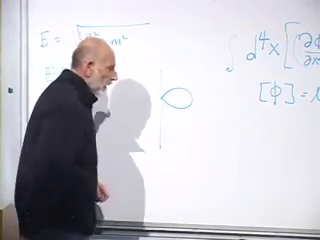
\includegraphics[width=0.72\textwidth]{lecture_03_figure_02.png}
\lectureframe{00:28:30.560}

\medskip
\begin{tikzpicture}[line width=0.8pt,scale=1.0]
  \draw[dashed] (-2.6,0) -- (0,0) -- (2.6,0);
  \fill (0,0) circle (0.055);
  \draw (0,0) .. controls (-0.85,0.7) and (-0.85,1.6) .. (0,1.6)
                .. controls (0.85,1.6) and (0.85,0.7) .. (0,0);
\end{tikzpicture}
\caption{스칼라 자기 에너지 논의로 넘어가는 순간의 칠판 모습과, 타드폴 도표의 위상만 보수적으로 다시 그린 그림이다. 스크린샷에서는 루프와 상대론적·질량 없는 에너지 식, 그리고 작용의 일부를 확실히 확인할 수 있다. 가려진 계수와 표기는 보인다고 주장하지 않는다.}
\end{figure}

꼭짓점에서 스칼라가 흡수되었다가 다시 방출되는 동안 다른 두 다리는 그 점에서 출발해 다시 그 점으로 전파될 수 있다. 수치 인자와 조합론적 인자를 제외하면 보정은 다음과 같다.
\begin{equation}
\delta m_\phi^2\sim \lambda G_\phi(0).
\end{equation}
연속체 근사에서 두 점이 일치하는 전파자는 발산한다. 유효 이론은 임의로 짧은 거리까지 유효하다고 주장하지 않으므로, \(|\Delta|\geq\delta\)을 부과하자. 그러면
\begin{equation}
G_\phi(0)\longrightarrow G_\phi(\delta)sim\frac{1}{\delta^2},
\qquad
\delta m_\phi^2\sim\frac{\lambda}{\delta^2}sim\lambda\Lambda^2.
\end{equation}
운동량 차단 척도의 제곱이 들어가므로 이 발산을 이차 발산이라 한다. 운동량 공간에서 적분해도 같은 결론을 얻는다. 지나치게 큰 기여는 한없이 큰 루프 운동량에서 나온다. 최단 거리 척도가 결국 대통일, 양자중력 또는 아직 상상하지 못한 무엇에 의해 정해지는지는 유효 이론의 진단을 바꾸지 않는다.

이는 미세 조정 문제다. \(\delta\)가 극도로 작고 \(\lambda\)가 특별히 미소한 값이 아니라면, 복사 보정은 저에너지에서 관측되는 스칼라 질량 제곱보다 훨씬 크다. 그러면 맨계수와 루프 보정이 믿기 어려울 정도로 많은 자릿수에서 상쇄되어야 한다.
\begin{equation}
m_{\mathrm{physical}}^2
=m_{\mathrm{bare}}^2+\delta m_\phi^2.
\end{equation}
질량이 있는 전파자라고 해서 문제가 해결되지는 않는다. 발산을 일으키는 거리에서는 \(e^{-m|\Delta|}\simeq1\)이다. 자외선 루프는 차단 척도에 도달하기 훨씬 전에 이미 질량을 무시한다.

\section{페르미온의 차원과 전파자}

이제 디랙 페르미온에 대해서도 같은 차원 분석을 해 보자. 자유 작용은 다음과 같다.
\begin{equation}
S_\psi=\int d^4x\,
\bar\psi\left(i\gamma^\mu\partial_\mu-m\right)\psi.
\end{equation}
감마 행렬은 수치로 이루어져 있으며 무차원이다. 운동항에는 미분이 하나만 포함되므로
\begin{align}
1
&=L^4[\bar\psi]L^{-1}[\psi],\\
[\psi]=[\bar\psi]&=L^{-3/2}.
\end{align}
반정수 거듭제곱을 보고 놀랄 필요는 없다. 페르미온 때문에 여러 곳에서 반정수가 나타난다.

\begin{classroomqa}
\audiencequestion{질량항으로 \([\psi]\)를 구하는 편이 더 쉽지 않은가? \lecturetimestamp{00:36:02}}
\lecturerresponse{그렇다. 질량항에서는 \(L^4L^{-1}[\bar\psi\psi]=1\)를 얻으므로, \([\bar\psi\psi]=L^{-3}\)이고 \([\psi]=L^{-3/2}\)이다. 질량이 없는 이론에서도 쓸 수 있고 페르미온 질량이 \(m\)로 나타나는 이유를 보여 주므로, 먼저 운동항을 이용해 유도했다. 페르미온 질량은 \(m^2\)로 나타나지 않는다.}
\end{classroomqa}

페르미온장 두 개의 차원은 \(L^{-3}\)이므로, 질량 없는 전파자에 대한 강의의 간결한 차원 표기는 다음과 같다.
\begin{equation}
S(\Delta)\sim\frac{1}{|\Delta|^3}.
\end{equation}
행렬 구조를 복원하면 로런츠 공변성에 필요한 더 정확한 분자가 나온다.
\begin{equation}
S_{ij}(\Delta)
\propto
\frac{\left(\gamma_\mu\Delta^\mu\right)_{ij}}
{\left(\Delta^2\right)^2}.
\end{equation}
분자에는 길이의 1승이 더해지므로 분모에는 간격의 4승이 들어간다. 전체 차원은 여전히 \(L^{-3}\)이다. 스칼라와 마찬가지로 페르미온 질량은 큰 분리 거리에서 전파자를 억제하지만, 단거리 스케일링은 바꾸지 않는다.

\section{닫힌 페르미온 루프의 부호가 음수인 이유}

이제 페르미온 도표가 문제가 되는 보손 자기 에너지를 상쇄할 수 있는지 물을 수 있다. 스칼라 타드폴의 부호는 \(\pi\)의 거듭제곱이나 조합론적 계수 같은 양의 수치 인자를 제외하면 양수다. 닫힌 페르미온 루프는 반대 부호를 갖는다.

\begin{classroomqa}
\audiencequestion{페르미온 루프의 음의 부호는 앞서 논의한 한 바퀴 회전과 관련이 있는가? \lecturetimestamp{00:40:21}}
\lecturerresponse{같은 페르미온 부호 구조와 관련은 있지만, 여기서는 루프의 기하학적 방향보다 입자 교환 반대칭성을 이용해 증명하는 편이 유용하다. 두 루프를 각각 자르고 동일한 입자들을 서로 교환한 다음 다시 연결하자. 두 루프가 하나로 합쳐지며, 그 교환은 페르미온에서만 음의 부호를 준다.}
\end{classroomqa}

전체 논증을 자세히 제시할 가치가 있다. 한 루프 도표의 부호가 \(\sigma\)이라고 하자. 부호는 양수일 수도 음수일 수도 있다. 서로 연결되지 않은 동일한 두 루프의 부호는 다음과 같다.
\begin{equation}
\sigma^2=+1.
\end{equation}
두 루프를 동시에 절단하자. 그러면 절단면 사이에서 동일한 두 입자가 전파된다. 통상적인 두 입자 파동함수는 보손의 경우 대칭이고 페르미온의 경우 반대칭이다:
\begin{align}
\Psi_B(x_1,x_2)&=+\Psi_B(x_2,x_1),\\
\Psi_F(x_1,x_2)&=-\Psi_F(x_2,x_1).
\end{align}
이 반대칭성은 파울리 원리도 설명한다. 두 페르미온을 같은 상태에 놓으면 서로 교환해도 물리적으로는 변함이 없지만, 파동함수의 부호는 반대가 되어야 하므로 파동함수는 사라진다.

두 입자를 교환한 뒤 절단된 선을 다시 연결하자. 위상적으로 두 루프는 하나가 된다. 교환하지 않은 두 루프 진폭은 양수였다. 교환해도 보손에서는 양의 부호가 유지되지만, 페르미온에서는 부호가 뒤집힌다. 따라서
\begin{equation}
\begin{aligned}
\operatorname{sign}(\text{closed boson loop})&=+1,\\
\operatorname{sign}(\text{closed fermion loop})&=-1.
\end{aligned}
\end{equation}
이는 일반적인 결론이다. 서로 독립적인 닫힌 페르미온 루프마다 \(-1\) 인자가 하나씩 붙는다.

\section{유카와 루프}

스칼라 질량으로 돌아가자. 페르미온 수 패리티가 달라지므로 보손 하나가 페르미온 하나로 바뀔 수는 없다. 가장 단순한 페르미온 보정에서는 스칼라가 페르미온과 반페르미온 쌍으로 갈라지고, 이 쌍이 루프를 따라 전파된 뒤 다시 결합한다. 이 상호작용은 유카와 결합으로 주어진다.
\begin{equation}
\mathcal L_Y=-g\phi\bar\psi\psi.
\end{equation}
힉스의 경우 페르미온은 쿼크나 렙톤일 수 있다. 상호작용점이 두 개이므로 \(g\) 인자도 두 개가 들어간다.

스칼라 타드폴에는 상호작용점이 하나 있었다. 병진 대칭성 때문에 시공간 부피만 곱해지므로 그 점의 전체 위치는 고정할 수 있었다. 유카와 루프에는 점이 두 개 있다. 한 점을 고정하거나, 같은 뜻으로 두 점의 평균 위치를 고정할 수는 있지만, 상대적 분리 \(\Delta\)에 대해서는 적분해야 한다. 각 페르미온 전파자가 단거리 인자 \(1/|\Delta|^3\)를 주므로,
\begin{equation}
\delta m_{\phi,F}^2
\sim
-g^2\int_{|\Delta|\geq\delta}d^4\Delta\,
\frac{1}{|\Delta|^6}.
\end{equation}

두 전파자와 분리 거리 적분, 두 결합을 적은 다음 마지막 인자를 강의실에 물었다. 답은 음의 부호다. 두 전파자가 닫힌 페르미온 루프를 이루므로, 나머지는 모두 양수인 단거리 적분 전체에 \(-1\)가 곱해진다.

발산은 차원 분석만으로 이미 결정된다. \(d^4\Delta\)에서 길이의 4승이 나오고 분모에는 6승이 들어가며, 남는 길이 척도는 차단 척도뿐이다.
\begin{equation}
\int_{|\Delta|\geq\delta}
\frac{d^4\Delta}{|\Delta|^6}
\sim\frac{1}{\delta^2}.
\end{equation}
사차원 유클리드 방사 좌표에서는 이를 명시적으로 나타낼 수 있다.
\begin{equation}
\int_{\delta}^{R}d^4\Delta\,\frac{1}{|\Delta|^6}
=2\pi^2\int_{\delta}^{R}dr\,\frac{r^3}{r^6}
=\pi^2\left(\frac{1}{\delta^2}-\frac{1}{R^2}\right).
\end{equation}
스피너의 대각합과 전파자 정규화는 계수를 바꾸지만 차단 척도에 대한 이차 거듭제곱은 바꾸지 않는다.\editorialnote{방사 적분은 강의에서 제시한 차원 추정을 명시적으로 나타낸 표준적인 예다. 양의 적분 측도와 자외선 거듭제곱 계수를 분명히 볼 수 있도록 유클리드 거리로 썼다.}

\begin{classroomqa}
\audiencequestion{적분 순서를 뒤집거나 적분 구간을 택하는 방식이 부호를 바꿀 수 있는가? \lecturetimestamp{00:51:06}}
\lecturerresponse{아니다. 물리적인 부호가 적분 한계에서 나오는, 방향을 가진 일차원 적분이 아니다. 네 성분에 대한 적분이며, 양의 방사 측도로 쓰면 더 분명하다. 자외선 기여의 크기는 양수다. 음의 기여는 닫힌 페르미온 루프에서만 나온다.}
\end{classroomqa}

\begin{classroomqa}
\audiencequestion{유카와 결합 \(g\)의 차원은 얼마인가? \lecturetimestamp{00:51:51}}
\lecturerresponse{사차원에서 무차원이다. \([\phi]=L^{-1}\)이고 \([\bar\psi\psi]=L^{-3}\)이므로, 곱 \(\phi\bar\psi\psi\)의 차원은 \(L^{-4}\)이다. 이 차원은 \(d^4x\)가 상쇄한다.}
\end{classroomqa}

따라서 페르미온의 주요 보정은 다음과 같다.
\begin{equation}
\delta m_{\phi,F}^2
\sim -C_F\frac{g^2}{\delta^2}
=-C_Fg^2\Lambda^2,
\end{equation}
여기서 \(C_F>0\)에는 수치 인자와 스핀, 다중도 인자가 들어간다. 스칼라 루프의 대응하는 식은 다음과 같다.
\begin{equation}
\delta m_{\phi,B}^2
\sim+C_B\frac{\lambda}{\delta^2}
=+C_B\lambda\Lambda^2.
\end{equation}
아직 미세 조정 문제를 해결하지는 못했지만, 반드시 필요한 사실 하나를 찾았다. 같은 자외선 차수를 가지면서 부호가 반대인 기여가 있다는 것이다.

\section{상쇄에 필요한 조건}

서로 무관한 결합 상수들이 큰 에너지 척도 계층에 필요한 정밀도만큼 정확히 다음 관계를 우연히 만족하는 것은 놀라운 우연일 것이다.
\begin{equation}
C_B\lambda=C_Fg^2
\end{equation}
강의에서는 관례에 따라 달라지는 인자와 다중도 인자를 생략하고 이를 \(g^2=\lambda\)로 줄여 쓴다. 진정한 해결책이라면 단지 그 관계를 허용하는 데 그치지 않고, 수학적 구조로 그 관계가 성립하도록 강제해야 한다.

이것이 초대칭의 동기다. 초대칭은 보손과 페르미온을 서로 연결하고, 위험한 발산 항 다수가 상쇄되도록 결합 상수의 조합을 제한한다. 이 상쇄는 매 루프마다 매개변수를 따로 조정해서 얻는 것이 아니라 대칭성에서 비롯되므로 여러 도표에서 반복된다.

질량의 일치도 중요하다. 보손과 페르미온의 질량이 같으면 전체 전파자를 가장 밀접하게 짝지을 수 있다. 질량이 조금 다르면 콤프턴 파장과 비슷한 거리에서 전파자가 서로 달라지므로 완전한 유한 기여는 정확히 상쇄되지 않는다. 그래도 두 전파자의 공통 단거리 점근 형태는 발산 부분을 상쇄할 수 있다.
\begin{equation}
\mathcal I_B(\Delta)-\mathcal I_F(\Delta)
\quad\hbox{may be finite as}\quad \Delta\to0,
\end{equation}
여기서 \(\mathcal I_B\)와 \(\mathcal I_F\)은 꼭짓점, 분자, 다중도를 포함한 보손 및 페르미온 루프 적분함수 전체를 뜻한다. 차원이 서로 다른 전파자 자체를 직접 빼는 것은 아니다. 자외선 항이 상쇄되어도 유한한 잔여항은 남을 수 있다. 이것이 근사 초대칭 또는 깨진 초대칭으로 이어지는 출발점이다. 정확한 질량 일치는 가장 깔끔한 상쇄를 준다. 충분히 제어된 대칭성 깨짐도 관측 가능한 질량 차이를 남기면서 자외선 재앙을 없앨 수 있다.

이제 초대칭의 대수 구조를 쓰기 전부터 초대칭에 이르렀다. 논리는 다음과 같이 완결된다.
\begin{equation}
\begin{gathered}
G_\phi(\Delta)\sim \Delta^{-2},
\qquad
\delta m_{\phi,B}^2\sim+C_B\lambda\Lambda^2,\\[0.4em]
S_\psi(\Delta)\sim \Delta^{-3},
\qquad
\delta m_{\phi,F}^2\sim-C_Fg^2\Lambda^2,\\[0.4em]
\text{symmetry-enforced matching}\\
\Longrightarrow\quad
\text{quadratic divergences cancel}.
\end{gathered}
\end{equation}
다음으로는 이러한 관계를 강제하는 추상적인 대칭성 원리를 이해하고, 그것이 어떻게 작용하는지 구체적인 예를 살펴보겠다.

\chapter{일반적인 대칭에서 그라스만 대수까지}

\lectureoverview{초대칭은 대칭의 한 종류이므로, 먼저 양자역학에서 대칭이라는 말이 무엇을 뜻하는지 되짚어 보자. 물리적 변환은 힐베르트 공간에서 유니터리 연산자로 표현된다. 연속 변환은 무한소 생성자로 나타내며, 생성자들의 교환자는 변환들이 어떻게 합성되는지를 담고 있다. 진정한 대칭은 에너지를 보존하며, 이는 해밀토니언과 교환한다는 것과 동등하다. 초대칭은 익숙한 모든 사례가 공유하는 한 가지 가정을 바꾼다. 초대칭 생성자는 보손을 페르미온으로, 페르미온을 보손으로 바꾼다. 이러한 생성자를 구성하다 보면 자연스럽게 생성·소멸 연산자와 반교환자, 그리고 홀수 원소의 제곱이 0이 되는 유한 그라스만 대수에 이르게 된다.}

\section{대칭은 서로 다른 배치를 연결한다}

대칭은 단지 보기 좋게 규칙을 맞춘 것이 아니다. 한 물리적 배치를 다른 배치와 연결하는 작용이다. 예를 들어 좌우 반사는 양손을 서로 연결한다. 사람과 주변의 법칙이 정확한 좌우 대칭을 가진다면, 양손의 대응하는 성질은 같을 것이다. 더 일반적으로, 정확한 대칭으로 연결된 물체나 상태는 그 대칭이 보존하는 물리량을 공유해야 한다. 입자물리학에서는 흔히 질량이 같고, 원자물리학에서는 같은 회전 다중항에 속하는 상태들의 에너지가 같다.

우리가 살펴볼 주제는 초대칭이지만, 먼저 회전이나 병진 같은 연속 대칭을 되짚어 보는 것이 유용하다. 초대칭이 통상적인 의미에서 “연속적”인지 묻는 것부터가 어색하다. 초대칭의 무한소 매개변수는 보통의 가환 실수가 아니기 때문이다. 초대칭은 연속 대칭의 등급화된 확장으로 보는 것이 가장 적절하며, 아래에서 도입할 그라스만 연산을 통해 이 말의 뜻을 지금 필요한 수준으로 정확히 표현할 수 있다. \editorialnote{현대 용어로 초대칭은 연속 등급 대칭이라고 한다. 이 한정어는 통상적인 연속 대 이산이라는 구분이 초대칭에는 깔끔하게 들어맞지 않는다는 강의의 설명을 보충한다.}

\section{힐베르트 공간에서의 유니터리 작용}

양자계는 상태 벡터 \(\ket{\psi}\)로 나타낸다. 물리적 대칭 작용은 그 상태에 작용하는 연산자 \(U\)로 표현된다:
\begin{equation}
\ket{\psi}\longmapsto U\ket{\psi}.
\end{equation}
공간 회전의 경우, 축과 각도가 \(U\)를 결정한다. 상태에 여러 위치의 입자가 포함되어 있다면, 변환된 켓은 모든 입자가 회전된 위치에 있는 배치를 나타낸다. 병진도 마찬가지로, 전체 배치가 이동된 상태로 원래 상태를 바꾼다.

\begin{classroomqa}
\audiencequestion{상태 벡터는 흔히 무한 차원인 힐베르트 공간에 속합니다. 힐베르트 공간을 회전하는 건가요, 아니면 보통의 3차원 공간을 회전하는 건가요? \lecturetimestamp{00:04:20}}
\lecturerresponse{두 설명은 서로 다른 수준에서 같은 작용을 가리킵니다. 유니터리 변환은 힐베르트 공간의 벡터에 작용하며, 보통 공간에서 배치가 물리적으로 회전하는 것을 나타냅니다. 추상적인 힐베르트 공간 자체를 문자 그대로 3차원 회전시키는 것이 아니라, 그 공간에서 공간 회전을 표현하는 것입니다.}
\end{classroomqa}

핵심 조건은 유니터리성이다:
\begin{equation}
U^\dagger U=UU^\dagger=\mathbf 1,
\qquad
U^{-1}=U^\dagger.
\end{equation}
이 조건은 내적을 보존하므로 확률도 보존한다:
\begin{equation}
\braket{U\psi}{U\psi}
=\bra{\psi}U^\dagger U\ket{\psi}
=\braket{\psi}{\psi}.
\end{equation}

\begin{figure}[H]
\centering
\includegraphics[width=0.56\textwidth]{lecture_04_figure_02.png}
\lectureframe{00:05:56.420}
\caption{변환된 상태에서 유니터리 조건으로 넘어가는 강의 초반의 판서. 켓과 수반 연산자의 곱은 보이지만 오른쪽 끝부분은 강사가 가리고 있다. 완전한 방정식은 아래 유도 과정에 나온다.}
\end{figure}

엄밀히 말하면 위그너 정리는 시간 반전처럼 반유니터리인 대칭도 허용한다. 여기서 다루는 항등 변환과 연속적으로 이어진 변환은 유니터리로 표현된다. \editorialnote{반유니터리 변환의 가능성은 표준적인 단서다. 이는 회전, 병진 또는 초대칭 생성자에 관한 강의의 설명을 바꾸지 않는다.}

\section{무한소 변환과 생성자}

아무 작용도 하지 않는 경우는 \(U=\mathbf 1\)로 나타내며, \(U=0\)로 나타내지 않는다. 충분히 작은 변환은 항등 연산자에서 작은 매개변수에 선형인 항만큼 달라진다. 작은 각도 \(\epsilon\)만큼 회전하면
\begin{equation}
U(\epsilon)=\mathbf 1+i\epsilon L+O(\epsilon^2).
\end{equation}
1차까지 유니터리이려면
\begin{align}
U^\dagger U
&=\left(\mathbf 1-i\epsilon L^\dagger\right)
  \left(\mathbf 1+i\epsilon L\right)+O(\epsilon^2)\\
&=\mathbf 1+i\epsilon(L-L^\dagger)+O(\epsilon^2),
\end{align}
따라서
\begin{equation}
L^\dagger=L.
\end{equation}
연산자 \(L\)가 무한소 생성자다.

회전에는 서로 독립인 축마다 하나씩, 세 생성자가 필요하다:
\begin{equation}
L_x,\qquad L_y,\qquad L_z.
\end{equation}
임의의 축 \(\widehat{\bm n}\)를 중심으로 하는 회전의 생성자는 다음과 같다:
\begin{equation}
L_{\widehat{\bm n}}=\widehat{\bm n}\cdot\bm L.
\end{equation}

\begin{classroomqa}
\audiencequestion{\(x\), \(y\), \(z\)축의 생성자를 더하면 다른 축을 중심으로 하는 회전을 만들 수 있나요? \lecturetimestamp{00:07:50}}
\lecturerresponse{그렇습니다. 이 생성자들의 선형결합은 그 사이 방향의 축을 중심으로 하는 회전을 생성합니다. 독립적인 성분 세 개면 모든 무한소 공간 회전을 만들 수 있습니다.}
\end{classroomqa}

회전의 경우 이 생성자는 각운동량의 성분이다. 이 표기가 더 일반적으로도 유용한 까닭은, 모든 연속 대칭을 국소적으로 생성자를 통해 이해하기 때문이다.

\section{곱셈표로서의 교환자}

회전 생성자는 다음 관계를 만족한다.
\begin{align}
[L_x,L_y]&=iL_z,&
[L_y,L_z]&=iL_x,&
[L_z,L_x]&=iL_y,
\end{align}
간결하게 쓰면,
\begin{equation}
[L_i,L_j]=i\epsilon_{ijk}L_k.
\end{equation}
두 지표가 같으면 레비치비타 기호는 사라지고, \(1,2,3\)의 순열이 짝순열이면 \(+1\), 홀순열이면 \(-1\)이다. 중요한 구조적 성질은 닫힘이다. 두 생성자의 교환자는 또 다른 생성자다.

교환자가 회전의 기하학을 어떻게 나타낼까? \(x\)축을 중심으로 작게 회전한 뒤, \(y\)축을 중심으로 회전하고, \(x\)축 회전을 되돌린 다음, 마지막으로 \(y\)축 회전을 되돌린다고 하자. 서로 다른 축을 중심으로 하는 회전은 가환하지 않으므로 작용들이 상쇄되지 않는다.

\begin{classroomqa}
\audiencequestion{비행기의 롤, 피치, 요로 이 비가환성을 그려 볼 수 있나요? \lecturetimestamp{00:12:36}}
\lecturerresponse{그렇습니다. 기체의 축을 중심으로 연속해서 회전하면 순서를 바꿨을 때 최종 방향이 달라진다는 사실을 곧바로 기하학적으로 확인할 수 있습니다. 아래 대수는 익숙한 이 사실의 무한소 형태입니다.}
\end{classroomqa}

다음을 두자.
\begin{equation}
U_x(\epsilon)=\mathbf 1+i\epsilon L_x,
\qquad
U_y(\delta)=\mathbf 1+i\delta L_y.
\end{equation}
연산자는 켓에 오른쪽에서 왼쪽으로 작용하므로, 말한 순서는 다음과 같이 표현된다:
\begin{equation}
\mathcal C
=U_y^{-1}(\delta)U_x^{-1}(\epsilon)
 U_y(\delta)U_x(\epsilon).
\end{equation}

\begin{classroomqa}
\audiencequestion{되돌리는 작용을 수반 연산자 대신 역연산자로 써도 되는 이유는 무엇인가요? \lecturetimestamp{00:13:25}}
\lecturerresponse{변환이 유니터리이기 때문입니다: \(U^\dagger=U^{-1}\). 무한소 변환의 역연산을 취하면 1차 항의 부호만 바뀝니다: \(U_x^{-1}=\mathbf 1-i\epsilon L_x+O(\epsilon^2)\).}
\end{classroomqa}

칠판에 적힌 네 인수를 곱하는 과정은 활기찬 연습이 되었다. \(\epsilon\) 또는 \(\delta\)에 일차인 항은 모두 상쇄되었고, 강의실에서는 혼합항을 함께 추적했다. 잠시 두 배 인수를 둘러싼 혼란이 생기면서 연산자 순서를 놓치기 얼마나 쉬운지가 드러났다. 정리된 이차 차수 결과는 다음과 같다.
\begin{align}
\mathcal C
&=\mathbf 1+\epsilon\delta[L_x,L_y]
  +O(\epsilon^2\delta,\epsilon\delta^2)\\
&=\mathbf 1+i\epsilon\delta L_z
  +O(\epsilon^2\delta,\epsilon\delta^2).
\end{align}
따라서 닫힌 순서를 따라 변환하면 \(z\)축 주위로 \(\epsilon\delta\)에 비례하는 각도만큼 작은 회전이 남는다. \editorialnote{칠판의 곱셈식은 강의실에서 계산을 탐색한 뒤 순서와 계수를 확정해 준다. 순서에 대한 규약을 뒤집으면 부호는 바뀌지만, 남는 변환이 교환자로 결정된다는 결론은 바뀌지 않는다.}

\begin{classroomqa}
\audiencequestion{역변환의 순서를 바꾸면 곱이 항등 연산자가 되나요? \lecturetimestamp{00:25:23}}
\lecturerresponse{각 변환을 자기 역변환 바로 옆에 놓으면 쌍마다 상쇄됩니다. 비자명한 교환자 순서에서는 의도적으로 그 쌍을 떨어뜨려 놓습니다. 이 순서에 따라 결과가 달라져 항등 변환으로 줄어들지 않는 정도가 순서 의존성을 나타냅니다.}
\end{classroomqa}

곱의 길이가 길어지면 계산은 더 복잡해지지만, 새로운 원리가 필요한 것은 아니다.

\begin{classroomqa}
\audiencequestion{생성자가 세 개보다 많거나 작은 변환을 여러 번 하면 어떻게 되나요? \lecturetimestamp{00:25:34}}
\lecturerresponse{교환자와 계산은 늘어나지만, 대수가 닫힌다는 것을 알면 무한히 많은 무한소 변환이 어떻게 결합되는지 알아낼 수 있습니다. 유한 변환은 작은 변환을 여러 번 합성해 만들 수 있습니다.}
\end{classroomqa}

이런 의미에서 교환자 대수는 항등 연산자 근방에서 연속군을 나타내는 곱셈표다.

\section{병진을 더해 공간의 예를 완성하다}

공간 병진의 생성자는 운동량이다. 강의에서 사용한 부호 규약에 따르면
\begin{equation}
\begin{aligned}
T_x(a)&=\mathbf 1+iaP_x+O(a^2),\\
T_y(b)&=\mathbf 1+ibP_y+O(b^2),
\end{aligned}
\end{equation}
여기서 \(a\)과 \(b\)은 각도가 아니라 거리다.

두 병진은 가환한다. 점을 먼저 \(x\) 방향으로, 다음에 \(y\) 방향으로 옮기고, \(x\) 방향 병진을 되돌린 뒤 \(y\) 방향 병진을 되돌리면 점은 원래 위치로 돌아온다:
\begin{equation}
[P_i,P_j]=0.
\end{equation}

\begin{classroomqa}
\audiencequestion{물체를 물리적으로 병진하거나 회전시키려면 운동을 시작하고 멈추게 하는 힘이 필요한가요? \lecturetimestamp{00:28:45}}
\lecturerresponse{여기서 정의하는 작용은 그런 것이 아닙니다. 대칭 변환은 원래 상태와 전체 배치가 병진 또는 회전한 수학적 상태를 비교합니다. 장치를 실제로 움직일 때의 동역학적 궤적이나 가속, 일의 양을 설명하는 것이 아닙니다.}
\end{classroomqa}

회전과 병진은 가환하지 않는다. 점을 병진한 뒤 원점을 중심으로 회전하고, 원래 축을 따라 다시 병진한 다음 회전을 되돌리면 점은 처음 위치로 돌아오지 않는다. 두 변환 생성자의 혼합 대수는 다음과 같다:
\begin{equation}
[L_i,P_j]=i\epsilon_{ijk}P_k.
\end{equation}
이 관계는 운동량 자체가 회전에 따라 벡터처럼 변환된다는 뜻이다. 여기서는 지수 계산을 일일이 따라가는 것보다 일반적인 교훈이 중요하다. 유클리드 공간의 변환은 회전 및 병진 생성자 사이의 교환자로 표현된다.

\section{대칭은 에너지를 보존해야 한다}

이제 변환의 합성에서 동역학으로 넘어가자. \(U\)가 어떤 계의 진정한 대칭이라면, 이를 적용해도 에너지는 바뀌지 않는다. \(\ket{E}\)를 에너지 고유상태라고 하자:
\begin{equation}
H\ket{E}=E\ket{E}.
\end{equation}
우변의 기호 \(E\)는 수이고, \(\ket{E}\)는 그 고윳값으로 표시되는 벡터다.

\begin{figure}[H]
\centering
\begin{minipage}[t]{0.43\textwidth}
\centering
\includegraphics[width=\linewidth]{lecture_04_figure_03.png}
\lectureframe{00:34:38.239}
\end{minipage}
\hfill
\begin{minipage}[t]{0.50\textwidth}
\centering
\includegraphics[width=\linewidth]{lecture_04_figure_04.png}
\lectureframe{00:36:22.376}
\end{minipage}
\caption{칠판의 연속된 화면에 변환된 켓 \(U\ket{E}\)과 정의를 이루는 고유값 방정식 \(H\ket{E}=E\ket{E}\)을 차례로 제시했다.}
\end{figure}

\(U\)가 대칭이면 \(U\ket{E}\)도 같은 고윳값을 갖는다:
\begin{equation}
HU\ket{E}=EU\ket{E}.
\end{equation}
\(E\)는 스칼라이므로 \(U\)와 교환한다. 따라서 원래 고윳값 방정식을 쓸 수 있다:
\begin{align}
HU\ket{E}
&=EU\ket{E}\\
&=UE\ket{E}\\
&=UH\ket{E}.
\end{align}
그러므로
\begin{equation}
(HU-UH)\ket{E}=0.
\end{equation}

\begin{classroomqa}
\audiencequestion{첫 번째 관계부터 유도를 다시 설명해 주시겠어요? \lecturetimestamp{00:35:55}}
\lecturerresponse{\(H\ket{E}=E\ket{E}\)에서 시작합니다. 대칭이므로 \(U\ket{E}\)도 같은 에너지를 가져서 \(HU\ket{E}=EU\ket{E}\)입니다. 스칼라 \(E\)를 \(U\) 너머로 옮기고, \(E\ket{E}\)를 \(H\ket{E}\)로 바꾼 다음 뺍니다. 그러면 \((HU-UH)\ket{E}=0\)가 됩니다.}
\end{classroomqa}

\begin{figure}[H]
\centering
\includegraphics[width=0.70\textwidth]{lecture_04_figure_05.png}
\lectureframe{00:38:51.066}
\caption{칠판에 전개한 전체 유도 과정. 곡선 안내 표시는 같은 에너지라는 진술에서 치환식 \(E\ket{E}=H\ket{E}\)으로 이어지며, 마지막 줄은 \((HU-UH)\ket{E}=0\)이다.}
\end{figure}

이 논증은 모든 에너지 고유상태에 대해 성립한다. 그 상태들이 완비 기저를 이룬다고 가정하면, 모든 기저 상태를 0으로 보내는 연산자는 영 연산자다:
\begin{equation}
[H,U]=0.
\end{equation}
이는 시간에 명시적으로 의존하지 않는 유니터리 변환이 해밀토니언의 대칭일 조건이다.

무한소 변환의 경우
\begin{equation}
U(\epsilon)=\mathbf 1+i\epsilon L_i+O(\epsilon^2),
\end{equation}
항등 연산자는 이미 \(H\)와 교환하므로, 각 생성자는 다음을 만족해야 한다:
\begin{equation}
[L_i,H]=0.
\end{equation}

\begin{figure}[H]
\centering
\includegraphics[width=0.47\textwidth]{lecture_04_figure_06.png}
\lectureframe{00:42:14.296}
\caption{칠판에 간결하게 정리한 대칭 조건은 \([U,H]=0\)이며, 이어서 생성자 형태를 제시했다. 아래쪽 라벨이 일부 흐릿해 \([L_i,H]=0\)로 표준화했다.}
\end{figure}

\(L_i\)가 시간에 명시적으로 의존하지 않으면 하이젠베르크 방정식은 다음과 같다:
\begin{equation}
\frac{dL_i}{dt}
=i[H,L_i]=0
\qquad(\hbar=1).
\end{equation}
따라서 대칭 생성자는 보존 전하이다. 공간 병진 대칭은 운동량 보존을, 회전 대칭은 각운동량 보존을 준다. \editorialnote{시간에 대한 명시적 편미분이 없다는 조건은 표준적인 단서이며, 강의에서 보존 법칙을 말할 때 암묵적으로 전제되어 있다.}

\section{전체 물리계를 변환하다}

“회전이 대칭이다”라는 말은 장치의 일부만 변환하면 잘못 쓰일 수 있다. 자유 스핀은 회전해도 에너지가 바뀌지 않는다. 그러나 고정된 자기장 안에 두고 스핀만 회전시키면 제만 에너지가 바뀐다. 이는 회전 대칭을 반박하는 것이 아니다. 스핀을 자기장에 대해 회전시키는 동안 자기장을 고정해 두었기 때문이다. 스핀과 자기장을 함께 회전시키거나, 그 자체로 불변인 외부장을 사용하면 에너지는 바뀌지 않는다.

수소 원자에서도 같은 문제가 나타난다. 양성자에 대해 전자만 병진시키면 두 입자 사이 거리가 바뀌므로 쿨롱 에너지도 달라진다. 병진 대칭은 전자와 양성자로 이루어진 전체 계에 작용해 둘을 같은 거리만큼 이동시킨다.

\begin{classroomqa}
\audiencequestion{외부장 자체도 대칭을 가져야 하나요? \lecturetimestamp{00:43:09}}
\lecturerresponse{고정된 외부장이 해당 작용에 대해 이미 불변이어야 합니다. 그렇지 않으면 계의 나머지 부분과 함께 외부장도 변환해야 합니다. 회전하지 않은 장에 대한 스핀의 상대적 회전은 전체 장치에 대칭 변환을 적용한 상태가 아니라 다른 물리적 배치입니다.}
\end{classroomqa}

원자의 회전 축퇴는 명확한 사례다. 각운동량 \(l\)가 고정되어 있으면 회전은 자기양자수가 다음 값을 갖는 상태들을 서로 섞는다:
\begin{equation}
m=-l,-l+1,\ldots,l.
\end{equation}
외부 자기장이나 전기장이 없을 때 다중항의 모든 상태는 에너지가 같다:
\begin{equation}
E_{l,m}=E_l.
\end{equation}
대칭은 서로 다른 상태들을 연결하며 이들의 축퇴를 강제한다.

\section{초대칭이 바꾸는 것}

지금까지 살펴본 익숙한 대칭은 모두 보손과 페르미온의 구별을 보존한다. 회전은 전자를 다른 전자로 보내지 광자로 바꾸지 않는다. 색 회전은 쿼크의 세 가지 색을 서로 섞지만 쿼크를 글루온으로 바꾸지는 않는다. 통상적인 내부 대칭과 시공간 대칭은 성분이나 양자수를 섞을 수 있지만, 그 생성자는 보손이며 페르미온 패리티를 바꾸지 않는다.

초대칭은 다르다:
\begin{equation}
Q\ket{B}\sim\ket{F},
\qquad
Q\ket{F}\sim\ket{B}.
\end{equation}
초대칭 다중항은 보손과 페르미온의 경계를 넘나든다. 정확한 초대칭 이론에서는 한 다중항의 초대칭 짝입자들이 같은 질량을 갖는다. 이는 앞선 강의들에서 살펴본 짝짓기 조건과 정확히 일치한다. 짝이 맞는 보손과 페르미온의 루프가 스칼라 질량에 대한 큰 자외선 보정을 상쇄할 수 있다. 보통의 공간 운동으로는 정수 스핀 상태를 반정수 스핀 상태로 바꿀 수 없으므로 초대칭을 시각적으로 그려 보기는 어렵다. 따라서 대수적으로 살펴보자.

\section{초전하의 원형}

\(A,A^\dagger\)를 보손의 소멸·생성 연산자, \(C,C^\dagger\)를 페르미온의 소멸·생성 연산자라고 하자. 보손과 페르미온의 한 입자 상태를 서로 바꾸는 가장 간단한 에르미트 연산자는 다음과 같다.
\begin{equation}
Q=C^\dagger A+A^\dagger C.
\end{equation}
첫째 항은 보손을 소멸시키고 페르미온을 생성하며, 둘째 항은 페르미온을 소멸시키고 보손을 생성한다. \(Q\)가 보손 하나로 이루어진 상태에 작용하면 소멸시킬 페르미온이 없으므로 \(A^\dagger C\) 항은 사라지고, \(C^\dagger A\)가 두 상태를 서로 바꾼다. 페르미온 하나로 이루어진 상태에서는 두 항의 역할이 서로 바뀐다.

\begin{classroomqa}
\audiencequestion{이 구성은 보손과 페르미온의 중첩 상태인 입자 하나를 만드는가? \lecturetimestamp{00:52:37}}
\lecturerresponse{\(Q\)는 상태가 아니라 연산자다. 순수한 보손 상태에 작용하면 페르미온 상태를 만들고, 순수한 페르미온 상태에 작용하면 보손 상태를 만든다. 이미 일반적인 중첩 상태인 벡터에 선형적으로 작용하면 또 다른 중첩 상태를 만든다. 이는 모든 선형 연산자에서 마찬가지다.}
\end{classroomqa}

이어 수강생들은 진공에 작용시켜 본다. 두 소멸 연산자가 모두 진공을 없애므로
\begin{equation}
A\ket{0}=0,\qquad C\ket{0}=0,
\end{equation}
따라서
\begin{equation}
Q\ket{0}=0.
\end{equation}
결과는 진공의 복사본이 아니라 영벡터다.

이 원형은 의도적으로 개략적인 형태다. 스핀 0 보손은 스핀 1/2 페르미온의 두 성분 중 어느 쪽으로도 대응될 수 있으므로 생성자 자체에 스피너 지수가 필요하다:
\begin{equation}
Q_\alpha\ket{B}\sim\ket{F_\alpha}.
\end{equation}
강의의 단순화된 2성분 그림에서는
\begin{equation}
Q_\alpha\ket{F_\beta}\sim\delta_{\alpha\beta}\ket{B}.
\end{equation}

\begin{classroomqa}
\audiencequestion{스핀 0 보손에는 스핀 성분이 하나이고 스핀 1/2 페르미온에는 둘인데, 상태 공간의 차원이 어떻게 맞을 수 있나요? \lecturetimestamp{00:55:02}}
\lecturerresponse{지수가 없는 \(Q\) 하나만으로는 충분하지 않습니다. 스피너 성분 \(Q_\alpha\)가 있어 각 성분이 페르미온의 스핀 성분 하나씩을 만들 수 있습니다. 스핀을 반 단위만큼 바꾸므로 초전하 자체도 스핀을 반 단위만큼 갖습니다.}
\end{classroomqa}

\(Q_\alpha\)는 페르미온 연산자, 더 정확히는 그라스만 홀수 연산자다. 각 항에는 페르미온 연산자가 홀수 개 들어 있으므로 페르미온 패리티를 뒤집는다. 일반적인 측정 가능 관측량은 짝수다. 홀수 초전하와 홀수 변환 매개변수는 구별해야 한다. 유한 초대칭 변환은 두 항 \(\epsilon\)와 \(Q\)가 모두 홀수인 \(\epsilon^\alpha Q_\alpha+\bar\epsilon_{\dot\alpha}\bar Q^{\dot\alpha}\) 같은 짝수 조합으로 구성된다. \editorialnote{강의에서는 생성자를 비공식적으로 그라스만 수라고 부른다. 더 정확히 말하면 초전하는 홀수 연산자이고, 반교환하는 매개변수가 그라스만 수다. 이들의 곱은 짝수이므로 유한 변환에 들어갈 수 있다.}

\section{보손과 페르미온 연산자 대수}

\(i,j\)로 표시되는 보손 모드에 대해
\begin{align}
[A_i,A_j]&=0,&
[A_i^\dagger,A_j^\dagger]&=0,&
[A_i,A_j^\dagger]&=\delta_{ij}.
\end{align}
생성 연산자들은 가환하므로
\begin{equation}
A_i^\dagger A_j^\dagger\ket{0}
=A_j^\dagger A_i^\dagger\ket{0}.
\end{equation}
두 보손 상태는 서로 바꾸어도 대칭이다.

페르미온 연산자는 반교환 관계를 만족한다.
\begin{align}
\{C_i,C_j\}&=0,&
\{C_i^\dagger,C_j^\dagger\}&=0,&
\{C_i,C_j^\dagger\}&=\delta_{ij},
\end{align}
여기서
\begin{equation}
\{X,Y\}=XY+YX.
\end{equation}
단일 모드에서는
\begin{equation}
\{C^\dagger,C^\dagger\}=2(C^\dagger)^2=0,
\end{equation}
따라서
\begin{equation}
(C^\dagger)^2=0.
\end{equation}
연산자 자체는 영이 아니지만 그 제곱은 영이다. 이 연산자는 해당 모드에 페르미온 하나를 생성할 수 있지만, 두 번째로 작용하면 결과가 영이 된다. 이것이 연산자 언어로 표현한 파울리 배타 원리다.

지수가 서로 다르면
\begin{equation}
C_i^\dagger C_j^\dagger\ket{0}
=-C_j^\dagger C_i^\dagger\ket{0},
\end{equation}
이는 두 페르미온 상태의 반대칭성을 뜻한다. 대수적으로 다음과 같이 바꾸면
\begin{equation}
\begin{gathered}
\text{bosons: commutators}\\
\Updownarrow\\
\text{fermions: anticommutators}
\end{gathered}
\end{equation}
통계적 차이가 표현된다.

한 모드에 여러 보손이 점유할 수 있다. 따라서 광자가 많이 점유된 상태는 보통의 수치 진폭을 갖는 고전적 전자기장처럼 거동할 수 있다. 페르미온은 한 모드에 쌓일 수 없으며, 페르미온 홀수 장은 보통의 가환하는 고전적 값을 갖지 않는다. 페르미온을 다룰 때는 이를 위해 다른 연산이 필요하다.

\section{그라스만 수와 패리티}

보통의 수는 가환한다:
\begin{equation}
\alpha_i\alpha_j=\alpha_j\alpha_i.
\end{equation}
그라스만 생성자는 반가환한다:
\begin{equation}
\theta_i\theta_j=-\theta_j\theta_i.
\end{equation}
\(i=j\)로 놓고, \(2\neq0\)인 수 체계를 쓰면
\begin{equation}
\theta_i^2=0.
\end{equation}
\(\theta_i\)에는 6이나 7 같은 보통의 수치값을 부여할 수 없다. 이 기호들은 페르미온의 부호를 추적하기 위해 만든 대수를 이룬다.

보통의 계수는 그라스만 생성자와 가환한다:
\begin{equation}
\alpha\theta_i=\theta_i\alpha.
\end{equation}

\begin{classroomqa}
\audiencequestion{보통의 수에 그라스만 수를 곱하면 어떤 종류의 대상이 되나요? \lecturetimestamp{01:12:32}}
\lecturerresponse{그 대상은 여전히 그라스만 홀수입니다. 보통의 계수를 곱하면 크기가 달라질 뿐 패리티는 바뀌지 않습니다. 생성자들의 선형생성 공간은 보통의 수를 체로 하는 벡터 공간입니다.}
\end{classroomqa}

이 대수에는 \(\mathbb Z_2\) 패리티가 있다. 보통의 계수와 생성자를 짝수 개 곱한 것은 짝수이고, 생성자 하나 또는 홀수 개를 곱한 것은 홀수다:
\begin{equation}
\begin{aligned}
\text{even}\cdot\text{even}&=\text{even},\\
\text{even}\cdot\text{odd}&=\text{odd},\\
\text{odd}\cdot\text{odd}&=\text{even}.
\end{aligned}
\end{equation}

\begin{classroomqa}
\audiencequestion{이것은 실수와 허수의 곱셈 규칙과 비슷한가요, 아니면 \(i\)를 도입하듯 일반화한 것인가요? \lecturetimestamp{01:14:25}}
\lecturerresponse{산술의 일반화이기는 하지만, 비유를 지나치게 밀어붙여서는 안 됩니다. 허수는 여전히 가환하고 \(i^2=-1\)를 만족하지만, 그라스만 홀수량은 반가환하며 제곱하면 0입니다. 짝수와 홀수가 곱해지는 양상이 같다고 해서 두 대수가 같은 것은 아닙니다.}
\end{classroomqa}

\(\theta_1\theta_2\)와 같은 곱은 짝수이며 그래스만 대수의 모든 동차 원소와 교환하지만, 보통의 수는 아니다. 이 곱은 영이 아니지만
\begin{equation}
(\theta_1\theta_2)^2=0.
\end{equation}

\begin{classroomqa}
\audiencequestion{\(\theta_1\theta_2\)가 짝수라면 왜 보통의 수가 아닌가? \lecturetimestamp{01:17:36}}
\lecturerresponse{짝수 패리티란 등급 대수에서 교환한다는 뜻이지, 실수나 복소수 스칼라라는 뜻은 아니다. 이 곱이 멱영원소라는 점만 보아도 영이 아닌 보통의 수와 다르다는 것을 알 수 있다.}
\end{classroomqa}

\section{그라스만 변수의 함수}

생성자가 하나이면 다항식은 일차항에서 끝난다.
\begin{equation}
f(\theta)=\alpha+\beta\theta.
\end{equation}
\(\theta^n\)은 \(n\geq2\)일 때 모두 영이다. 생성자가 둘이면 가장 일반적인 원소는 다음과 같다.
\begin{equation}
f(\theta_1,\theta_2)
=\alpha+\beta_1\theta_1+\beta_2\theta_2
+\gamma\theta_1\theta_2.
\end{equation}
마지막 단항식의 순서를 뒤집어 쓰면 부호가 바뀐다.
\begin{equation}
\theta_2\theta_1=-\theta_1\theta_2.
\end{equation}

\begin{classroomqa}
\audiencequestion{\(\theta_1\)에 계수 \(\beta\)를 곱하면 독립적인 그라스만 변수가 하나 더 생기나요? \lecturetimestamp{01:18:39}}
\lecturerresponse{아닙니다. \(\theta_1\)의 선형생성 공간 안에 벡터가 하나 더 생길 뿐, 새로운 기저 생성자가 추가되는 것은 아닙니다. 독립적인 생성자가 두 개일 때 모든 홀수 선형항은 \(\beta_1\theta_1+\beta_2\theta_2\)입니다.}
\end{classroomqa}

생성자가 셋이면 순서가 정해진 기저는 다음과 같다.
\begin{equation}
1,\quad
\theta_1,\theta_2,\theta_3,\quad
\theta_1\theta_2,\theta_1\theta_3,\theta_2\theta_3,\quad
\theta_1\theta_2\theta_3.
\end{equation}
일반적으로 생성자가 \(n\)개이면 순서가 정해진 기저 단항식 \(2^n\)개가 생긴다. 유한 개의 그래스만 생성자로 이루어진 임의의 해석적 함수는 다항식에서 끝난다. 같은 생성자가 반복해서 나타나는 항은 사라지기 때문이다. \editorialnote{\(2^n\)차원 기저는 강의에서 생성자가 하나, 둘, 셋일 때 차례로 구성한 패턴을 명시적으로 보여 준다.}

\section{그라스만 미분}

변수가 하나일 때 다음과 같이 정의한다:
\begin{equation}
\frac{\partial}{\partial\theta}\alpha=0,
\qquad
\frac{\partial}{\partial\theta}\theta=1,
\end{equation}
그러면
\begin{equation}
\frac{\partial}{\partial\theta}
(\alpha+\beta\theta)=\beta.
\end{equation}
변수가 둘일 때는 왼쪽 미분을 택하고 표준 순서 \(\theta_1\theta_2\)를 유지하면
\begin{align}
\frac{\partial^L f}{\partial\theta_1}
&=\beta_1+\gamma\theta_2,\\
\frac{\partial^L f}{\partial\theta_2}
&=\beta_2-\gamma\theta_1.
\end{align}
둘째 줄의 마이너스 부호는 홀수 미분 연산자가 \(\theta_1\)를 지나 \(\theta_2\)를 미분해야 해서 생긴다.

이를 등급화된 곱의 미분 법칙으로 나타낼 수 있다. \(A\)의 패리티가 \(|A|\in\{0,1\}\)라면
\begin{equation}
\frac{\partial^L}{\partial\theta}(AB)
=\left(\frac{\partial^L A}{\partial\theta}\right)B
+(-1)^{|A|}A
\left(\frac{\partial^L B}{\partial\theta}\right).
\end{equation}
이 법칙은 기본적으로 보통의 미분법과 같지만, 반교환성에 따른 부호가 들어간다. 그라스만 적분도 정의할 수 있고, 함수 공간이 유한하므로 간단한 표로 정리된다. 강의에서는 그 표를 뒤로 미룬다.

\section{지수함수의 수수께끼를 풀다}

그래스만 생성자가 하나이고 보통의 계수가 \(a\)일 때,
\begin{equation}
e^{a\theta}
=1+a\theta,
\end{equation}
더 높은 거듭제곱은 모두 영이기 때문이다. 같은 생성자를 포함하는 두 지수함수는 다음 관계를 만족한다.
\begin{align}
e^{a\theta}e^{b\theta}
&=(1+a\theta)(1+b\theta)\\
&=1+(a+b)\theta\\
&=e^{(a+b)\theta}.
\end{align}

이어서 수업에서는 서로 다른 생성자들을 다뤄 본다. 직접 곱하면
\begin{equation}
e^{\theta_1}e^{\theta_2}
=(1+\theta_1)(1+\theta_2)
=1+\theta_1+\theta_2+\theta_1\theta_2.
\end{equation}
처음에 칠판의 전개를 보면 \(\theta_1+\theta_2\)의 제곱이 마지막 항을 만들 것처럼 보인다. 한 수강생이 부호를 지적한다:
\begin{equation}
(\theta_1+\theta_2)^2
=\theta_1^2+\theta_1\theta_2
 +\theta_2\theta_1+\theta_2^2
=0.
\end{equation}

\begin{classroomqa}
\audiencequestion{제곱항에 \(\theta_1\theta_2+\theta_2\theta_1\)가 들어 있어서 상쇄되나요? \lecturetimestamp{01:24:00}}
\lecturerresponse{그렇습니다. 이 수정으로 결론이 달라집니다: \(e^{\theta_1+\theta_2}=1+\theta_1+\theta_2\)인 한편, 순서가 정해진 곱 \(e^{\theta_1}e^{\theta_2}\)에는 \(\theta_1\theta_2\)도 들어 있습니다. 서로 반교환하는 지수의 경우에는 단순한 지수 덧셈 법칙이 성립하지 않습니다.}
\end{classroomqa}

모순은 없다. 보통의 행렬도 \(e^Ae^B=e^{A+B}\)는 \(A\)과 \(B\)이 가환할 때만 성립한다. 여기서는
\begin{equation}
[\theta_1,\theta_2]
=\theta_1\theta_2-\theta_2\theta_1
=2\theta_1\theta_2.
\end{equation}
이 교환자는 짝수이고 두 생성자 모두와 가환하므로, 바커–캠벨–하우스도르프 급수는 다음에서 끝난다:
\begin{equation}
e^{\theta_1}e^{\theta_2}
=\exp\left(
\theta_1+\theta_2+\frac12[\theta_1,\theta_2]
\right)
=e^{\theta_1+\theta_2+\theta_1\theta_2}.
\end{equation}
우변의 지수가 멱영이므로 정확히 다음과 같이 전개된다:
\(1+\theta_1+\theta_2+\theta_1\theta_2\). \editorialnote{이 BCH 계산은 실시간 강의에서 의문으로 남겨 둔 문제를 해결한다. 강의에서는 단순한 법칙이 성립하지 않는다는 점을 올바르게 알아냈지만, 누락된 교환자 항을 찾기 전에 끝난다.}

\begin{classroomqa}
\audiencequestion{\(1+\theta_1\)는 어떤 종류의 수인가요? 보통의 부분과 그라스만 부분을 더해도 되나요? \lecturetimestamp{01:26:16}}
\lecturerresponse{그것은 그라스만 대수의 비동차 원소이며, 짝수 부분 \(1\)와 홀수 부분 \(\theta_1\)를 갖습니다. 이러한 합은 허용되지만, 보통의 스칼라도 아니고 동차 홀수 원소도 아닙니다.}
\end{classroomqa}

강의가 끝나갈 무렵, 또 다른 겉보기 역설을 살펴본다.
\begin{equation}
(\theta_1+\theta_2)^2=0.
\end{equation}
그렇다고 해서 \(\theta_1\theta_2=0\)라는 뜻은 아니다. 두 교차항은 각각 사라지는 것이 아니라 서로 상쇄되기 때문이다.

\begin{classroomqa}
\audiencequestion{모든 홀수 Grassmann 원소의 제곱이 영이라면, 임의의 두 Grassmann 생성자의 곱도 영이라는 뜻인가요? \lecturetimestamp{01:32:19}}
\lecturerresponse{아닙니다. 방정식 \((\theta_1+\theta_2)^2=0\)은 \(\theta_1\theta_2+\theta_2\theta_1=0\)을 뜻합니다. 이는 반교환 관계를 증명할 뿐, 두 순서 있는 곱 중 어느 하나가 영임을 뜻하지는 않습니다. 서로 다른 생성자끼리의 곱은 영이 아닐 수 있습니다.}
\end{classroomqa}

\begin{classroomqa}
\audiencequestion{이 지수함수들을 쓸 때 보통의 멱급수 정의를 가정하나요? \lecturetimestamp{01:34:42}}
\lecturerresponse{그렇습니다. 모든 급수가 유한한 항에서 끝나므로 그 정의는 일관됩니다. 문제가 되는 것은 지수함수 자체가 아니라, 교환하지 않는 \(A\)과 \(B\)에 대해 항등식 \(e^Ae^B=e^{A+B}\)을 정당한 근거 없이 적용하는 것입니다. 교환자 보정항을 포함하면 올바른 합성 법칙이 복원됩니다.}
\end{classroomqa}

이 탐색적인 마무리는 적절합니다. 보통의 대칭성을 살펴보며 유니터리 변환에서 생성자와 교환자로 나아갔고, 초대칭성을 살펴보며 홀수 생성자에서 반교환 변수로 나아갔습니다. 두 경우 모두 곱셈 법칙이 핵심입니다. 회전에서는 \([L_i,L_j]\)에 나타나고, 그래스만 지수함수에서는 단순한 덧셈을 막는 교환자 항에 나타납니다. 이 대수는 낯설지만, 일관되고 유한하며 초대칭성이 요구하는 페르미온 변환에 정확히 들어맞습니다.

\chapter{초전하, 대수의 닫힘, 초공간}

\lectureoverview{초대칭이 어려운 까닭은 규칙이 많아서가 아니라, 보통의 물리학에서는 서로 분리해 다루는 개념들을 그 규칙들이 하나로 엮기 때문이다. 먼저 홀수 원소끼리 반가환하고 함수 전개가 유한한 항에서 끝나는 그래스만 변수를 살펴본다. 이 변수의 미분 대수는 홀수 대칭 생성자의 모형을 제공한다. 보손 조화진동자와 페르미온 조화진동자를 결합하면 가장 단순한 초전하를 얻는다. 초전하의 반교환자가 해밀토니안이므로 보손과 페르미온의 교환은 시간 병진과 분리될 수 없다. 같은 대수는 초공간이라 부르는 확장된 시공간의 그래스만 방향으로 병진하는 기하학적 방식으로도 표현할 수 있다.}

\section{앞으로 나아가기 전에 되짚어야 하는 이유}

초대칭은 물리학에서 가장 추상적인 구성 가운데 하나다. 대칭이라는 점에서는 회전이나 병진과 비슷하지만, 좌표의 의미를 확장하지 않고서는 보통의 시공간 안에 담을 수 없다. 초대칭의 자연스러운 매개변수는 그래스만 양이다. 이들은 더하고 곱할 수 있지만, 교환법칙을 따르는 대신 서로 반가환한다.

따라서 최종 대수부터 바로 다루는 것은 도움이 되지 않는다. 먼저 홀수 산술을 다룰 수 있게 정리하고, 보통의 연속 대칭이 어떻게 구성되는지 되짚은 다음, 두 개념을 결합한다. 과정은 길지만 각 단계가 다음 단계를 준비한다.

\section{그래스만 대수를 실제 계산에 활용하기}

\subsection{홀수 원소와 짝수 원소}

독립적인 그래스만 생성자를 \(\epsilon_i\)라 하자. 이들은 다음 관계를 만족한다.
\begin{equation}
\epsilon_i\epsilon_j=-\epsilon_j\epsilon_i,
\qquad
\{\epsilon_i,\epsilon_j\}=0.
\end{equation}
\(i=j\)로 놓으면 실수체나 복소수체에서
\begin{equation}
2\epsilon_i^2=0,
\qquad
\epsilon_i^2=0,
\end{equation}
가 성립한다. 생성자가 0인 것은 아니다. 제곱만 0이다.

각 동차 원소에는 짝홀성이 있다. 그래스만 생성자가 홀수 개 들어간 곱은 홀수이고, 짝수 개 들어간 곱은 짝수다.
\begin{align}
\text{odd}\times\text{odd}&=\text{even},\\
\text{odd}\times\text{even}&=\text{odd},\\
\text{even}\times\text{even}&=\text{even}.
\end{align}
짝수 원소는 동차 원소와 가환한다. 두 홀수 원소는 반가환한다. 따라서
\begin{equation}
n\epsilon_i=\epsilon_i n,
\qquad
\epsilon_i\epsilon_j=-\epsilon_j\epsilon_i,
\end{equation}
\(n\)가 짝수일 때 성립한다.

짝수 원소가 보통의 실수나 복소수일 필요는 없다. 예를 들어 곱 \(\epsilon_1\epsilon_2\)은 짝수이면서 멱영이다. 보통의 수는 대수의 스칼라 부분을 이루고, 짝수 원소의 곱은 그 밖에도 가환하는 원소를 제공한다.

\begin{classroomqa}
\audiencequestion{그래스만 대수와 그래스만 수는 구별되는 건가요, 아니면 같은 건가요? \lecturetimestamp{00:06:45}}
\lecturerresponse{그래스만 수는 대수의 원소이고, 대수는 그 원소들과 덧셈 및 곱셈 규칙을 함께 모아 놓은 것이다. 그러므로 느슨하게는 같은 대상을 가리킨다고 해도 되지만, 다루는 대상과 그것을 다루는 규칙을 구별해 두면 유용하다.}
\end{classroomqa}

\subsection{유한한 차수에서 끝나는 함수}

그래스만 변수 하나의 함수에는 가능한 거듭제곱이 두 개뿐이다.
\begin{equation}
f(\epsilon)=a+b\epsilon.
\end{equation}
\(\epsilon^2\)항은 없다. 서로 독립인 생성자 두 개가 있으면
\begin{equation}
f(\epsilon_1,\epsilon_2)
=a+b_1\epsilon_1+b_2\epsilon_2+c\epsilon_1\epsilon_2.
\end{equation}
두 생성자가 모두 나타나는 항에서 전개가 끝난다. 독립 생성자가 \(n\)개라면 순서가 정해진 단항식들이 \(2^n\)차원 기저를 이룬다.
\begin{equation}
1,\quad
\epsilon_i,\quad
\epsilon_i\epsilon_j,\quad
\ldots,\quad
\epsilon_1\epsilon_2\cdots\epsilon_n.
\end{equation}
\editorialnote{유한한 \(2^n\)차원이라는 이 명제가 생성자가 하나 또는 둘인 경우를 일반화한 것이다. 무한 그래스만 대수도 정의할 수 있지만, 여기서 쓰는 모든 다항식에는 유한 개의 생성자만 들어간다.}

실수 생성자 두 개를 복소수 쌍 \(\theta,\bar\theta\)으로 결합하면, 순서를 정했을 때 일반적인 함수는 다음과 같이 쓸 수 있다.
\begin{equation}
f(\theta,\bar\theta)
=a+\bar b\,\theta+\bar\theta\,b+c\,\bar\theta\theta.
\end{equation}
위의 막대 표기는 여기서 쓰는 복소수 쌍 표기다. 마지막 두 항의 순서를 바꾸면 부호가 달라진다.
\begin{equation}
\bar\theta\theta=-\theta\bar\theta.
\end{equation}

보통은 함수 전체에 명확한 짝홀성을 부여하는 편이 편리하다. \(f\)가 짝수라면 \(a\)와 \(c\)는 짝수이고, \(b\)와 \(\bar b\)는 홀수다. \(f\)가 홀수라면 짝홀성은 반대로 정해진다. 계수는 전개에 사용하는 해당 변수들에 의존하지 않는 한, 더 큰 그래스만 대수의 원소여도 된다.

\begin{classroomqa}
\audiencequestion{그래스만 변수를 삼각함수나 다른 해석함수에 넣어도 되나요? \lecturetimestamp{00:11:06}}
\lecturerresponse{가능하다. 다만 멱급수는 곧바로 끝난다. 홀수 생성자 하나에 대해서는
\[
\sin\epsilon=\epsilon,\qquad
\cos\epsilon=1,\qquad
e^\epsilon=1+\epsilon.
\]
익숙한 함수 이름은 그대로 쓰지만, 함수가 통상적인 해석적 복잡성을 띨 만큼 항이 충분하지 않다.}
\end{classroomqa}

\section{미분은 부호를 추적하는 일}

왼쪽 그래스만 미분을 사용한다. 미분의 국소적인 정의 규칙은 다음과 같다.
\begin{equation}
\partial_\theta a=0,
\qquad
\partial_\theta(\theta B)=B,
\end{equation}
여기서 \(a\)와 \(B\)는 \(\theta\)에 의존하지 않는다. 미분하기 전에 관련된 \(\theta\)를 왼쪽으로 옮긴다. 다른 홀수 인자를 하나 지날 때마다 부호가 바뀐다.

예를 들어 \(b\)가 홀수라면
\begin{equation}
b\theta=-\theta b,
\qquad
\partial_\theta(b\theta)=-b.
\end{equation}
미분에 특별한 일이 일어난 것은 아니다. 홀수 인자들의 순서를 바꿀 때 미분하기 전에 마이너스 부호가 생긴 것이다.

\subsection{변수 두 개를 사용한 계산}

다음을 다시 살펴보자.
\begin{equation}
f(\theta,\bar\theta)
=a+\bar b\,\theta+\bar\theta\,b+c\,\bar\theta\theta.
\end{equation}
먼저 \(f\)가 짝수라고 하자. 그러면 \(\bar b\)는 홀수이고 \(c\)는 짝수다. \(\theta\)가 들어 있는 항들의 순서를 바꾸면
\begin{align}
\bar b\,\theta&=-\theta\bar b,\\
c\,\bar\theta\theta&=-\theta c\,\bar\theta.
\end{align}
따라서
\begin{equation}
\partial_\theta f=-\bar b-c\bar\theta.
\end{equation}

\(f\)가 홀수라면 \(\bar b\)는 짝수이고 \(c\)는 홀수다. 첫 번째 항은 홀수 계수를 지나지 않지만, 마지막 항의 \(\theta\)는 두 홀수 인자 \(c\)와 \(\bar\theta\)를 지난다. 두 번 부호가 바뀌어 상쇄된다.
\begin{equation}
\partial_\theta f=\bar b+c\bar\theta.
\end{equation}

\begin{classroomqa}
\audiencequestion{짝수인 경우 살아남는 두 항에 모두 마이너스 부호가 붙는 이유는 무엇인가요? \lecturetimestamp{00:16:49}}
\lecturerresponse{첫 번째 부호는 \(\theta\)를 홀수 계수 \(\bar b\) 너머로 옮길 때 생긴다. 마지막 항에서 \(c\)는 짝수지만, \(\theta\)는 홀수 변수 \(\bar\theta\)를 지나야 한다. 각 순서 교환에서 홀수 인자 하나를 지나므로 마이너스 부호가 하나씩 생긴다.}
\end{classroomqa}

답은 순서 규약에 따라 달라지지만 수학은 달라지지 않는다. \(c\bar\theta\theta\) 대신 \(c\theta\bar\theta\)로 시작했다면, 식에 표시되는 계수의 부호가 달라지고 미분 공식도 그에 맞게 바뀐다.

\begin{classroomqa}
\audiencequestion{마지막 항을 \(\theta\)와 \(\bar\theta\)의 순서를 바꾸어 써도 되나요? 그렇게 했을 때 생기는 부호에는 더 깊은 의미가 있나요? \lecturetimestamp{00:18:50}}
\lecturerresponse{어느 순서로든 쓸 수 있지만, 두 홀수 변수를 교환하면 부호가 바뀐다. 그 부호는 계수 \(c\)에 흡수할 수 있다. 여기서는 그 효과가 부호를 추적하는 절차에 해당한다. 순서는 중요하지만 짝홀성은 바뀌지 않으며, 부호가 바뀌어도 홀수 원소가 짝수 원소로 변하지 않는다. 이러한 부호 추적이 페르미온 통계와 초대칭을 구현할 때 물리적 의미를 갖는다.}
\end{classroomqa}

\begin{classroomqa}
\audiencequestion{계수 \(a,b,c\)는 단순히 복소수체에서 가져오나요? \lecturetimestamp{00:20:47}}
\lecturerresponse{필요한 짝홀성이 짝수라면 보통의 복소수일 수 있지만, 선택한 \(\theta,\bar\theta\) 이외의 생성자를 포함할 수도 있다. 관심을 두는 대수에는 보통 모든 복소 스칼라와 선택된 홀수 생성자 및 그 곱이 들어간다.}
\end{classroomqa}

\begin{classroomqa}
\audiencequestion{짝수 함수와 홀수 함수의 미분 결과가 서로 반대처럼 보입니다. 일반적인 대칭 관계인가요? \lecturetimestamp{00:22:31}}
\lecturerresponse{그 자체로는 그렇지 않다. 부호는 각 계수의 짝홀성과 지나치는 홀수 인자의 개수에 따라 기계적으로 정해진다. 때로 두 답이 우연히 서로 반대가 되기도 하지만, 믿고 따를 규칙은 더 간단하다. 홀수 원소 두 개를 교환할 때마다 마이너스 부호가 붙는다.}
\end{classroomqa}

\subsection{좌표와 미분 연산자}

보통의 연산자에서도 비슷한 사례를 볼 수 있다. \(x\)를 곱하는 연산자와 \(x\)에 대한 미분 연산자가 임의의 함수 \(g(x)\)에 작용한다고 하자. 그러면
\begin{align}
\partial_x\!\left(xg\right)&=g+xg',\\
x\partial_xg&=xg',
\end{align}
따라서
\begin{equation}
[\partial_x,x]g=g.
\end{equation}
이 관계가 모든 \(g\)에 대해 성립하므로
\begin{equation}
[\partial_x,x]=1.
\end{equation}
\(p=-i\partial_x\)를 대입하면 \(\hbar=1\) 단위계에서 익숙한 위치-운동량 대수를 얻는다.

그래스만 변수에 해당하는 관계는 반교환자를 사용한다. 다음과 같이 놓자.
\begin{equation}
f(\theta)=a+\theta b,
\end{equation}
여기서 \(a\)는 짝수이고 \(b\)는 홀수이므로 \(f\)는 짝수다. 먼저
\begin{equation}
\theta\partial_\theta f=\theta b.
\end{equation}
반대 순서로 작용시키면
\begin{align}
\partial_\theta(\theta f)
&=\partial_\theta(\theta a+\theta^2b)\\
&=a.
\end{align}
두 순서를 더하면 원래 함수가 된다.
\begin{equation}
\left(\partial_\theta\theta+\theta\partial_\theta\right)f
=a+\theta b=f.
\end{equation}
따라서
\begin{equation}
\boxed{\{\partial_\theta,\theta\}=1.}
\end{equation}
미분 연산자 \(\partial_\theta\) 자체는 홀수다. 그래서 홀수 좌표와의 정준 관계가 반교환자로 주어진다.

\begin{classroomqa}
\audiencequestion{짝수 부분과 홀수 부분을 함께 포함하여 짝홀성이 정해지지 않은 함수를 써도 되나요? \lecturetimestamp{00:31:05}}
\lecturerresponse{이처럼 비동차 원소를 만들 수는 있지만, 보통 계산은 동차인 짝수 및 홀수 원소별로 구성한다. 짝홀성이 명확하면 등급이 있는 곱에서 모든 부호가 명확해진다. 혼합 원소는 짝수 부분과 홀수 부분으로 나누어 다룬다.}
\end{classroomqa}

\begin{classroomqa}
\audiencequestion{보통의 교환자 계산에서 시험 함수 \(g(x)\)도 홀수라고 가정한 건가요? \lecturetimestamp{00:31:45}}
\lecturerresponse{아니다. 그것은 보통의 가환 좌표에 대한 보통의 함수였다. 그래스만 변수 쌍 \(\partial_\theta,\theta\)을 사용해 논증을 반복하기 전에 연산자 항등식 \([\partial_x,x]=1\)을 어떻게 증명하는지 보이기 위해 도입했을 뿐이다.}
\end{classroomqa}

\begin{classroomqa}
\audiencequestion{독립 그래스만 생성자의 개수에 한계가 있나요? \lecturetimestamp{00:32:16}}
\lecturerresponse{대수적으로 상한은 없다. 생성자가 \(n\)개이면 기저에 단항식이 \(2^n\)개 있으므로 부호를 추적하는 일이 빠르게 늘어나지만, 구성 자체는 유한한 임의의 \(n\)에 대해 성립한다.}
\end{classroomqa}

\subsection{적분}

그래스만 변수 하나에 대한 적분은 다음과 같이 정의한다.
\begin{equation}
\int d\theta\,1=0,
\qquad
\int d\theta\,\theta=1.
\end{equation}
따라서 \(f(\theta)=a+\theta b\)일 때
\begin{equation}
\int d\theta\,f(\theta)=b=\partial_\theta f(\theta).
\end{equation}
적분과 미분은 같은 성분을 추출한다. 이것이 베레진 적분이다. 이 정규화는 병진 불변성과 그래스만 부분적분에 부합하는 유일하고 간단한 선택이다. \editorialnote{성분별 규칙은 그래스만 적분과 미분이 같은 연산이라는 강의의 설명을 구체적으로 보여 준다.}

\section{기준이 되는 보통의 대칭}

에르미트 생성자 \(G_i\)를 갖는 연속 유니터리 군을 생각하자. 항등원 근처에서는
\begin{equation}
U(\alpha)=\mathbf 1+i\alpha^iG_i+O(\alpha^2),
\end{equation}
여기서 \(\alpha^i\)는 보통의 가환 매개변수다. 무한소 곱셈 법칙은 다음 리 대수로 표현된다.
\begin{equation}
[G_i,G_j]=i f_{ij}{}^{k}G_k.
\end{equation}
상수 \(f_{ij}{}^k\)는 구조 상수다. 닫힘이란 임의의 두 생성자를 교환했을 때 그 결과가 이미 대수에 속하는 생성자들의 선형결합으로 주어짐을 뜻한다.

회전의 경우
\begin{equation}
[L_i,L_j]=i\varepsilon_{ijk}L_k.
\end{equation}
세 에르미트 성분을 비에르미트 승강 및 강하 연산자로 결합할 수 있다.
\begin{equation}
L_\pm=L_x\pm iL_y,
\end{equation}
이 연산자들은 자기 양자수 \(m\)를 1만큼 올리거나 내린다. 복소수 선형결합은 바탕이 되는 물리적 생성자의 에르미트성을 바꾸지 않으면서 유용하게 쓰인다.

일반적인 기저에서 \(f_{ij}{}^k\)의 처음 두 지수만 반대칭이어야 한다. 불변 직교 계량을 갖는 콤팩트 대수에서는 마지막 지수를 내리고 규약을 선택하여 \(f_{ijk}\)가 완전히 반대칭이 되게 할 수 있다. 회전의 경우가 그러하다. \editorialnote{이 단서는 모든 경우에 성립하는 교환자의 반대칭성과 익숙한 회전 기저에서 성립하는 더 강한 성질을 구별한다.}

시간에 의존하지 않는 계의 실제 대칭을 \(G_i\)가 생성하려면
\begin{equation}
[H,G_i]=0.
\end{equation}
이어야 한다. 같은 말로, \(G_i\)는 모든 에너지 고유공간을 그 자체로 사상한다. 시간에 대한 명시적 의존성이 없을 때 하이젠베르크 방정식은
\begin{equation}
\frac{dG_i}{dt}=i[H,G_i]=0,
\end{equation}
을 주므로 생성자는 보존 전하가 된다.

보통의 관측가능량은 짝수다. 페르미온 장은 홀수지만, 홀수 장 하나만으로는 측정 가능한 관측가능량이 되지 않는다. 물리적 연산자에는 페르미온 인자가 총 짝수 개 들어간다. 초대칭은 생성자의 짝홀성을 바꾸지만, 관측 가능한 결과에 요구되는 짝홀성은 바꾸지 않는다.

모든 경우를 간결하게 표기하려면 등급 교환자를 사용한다.
\begin{equation}
[X,Y]_{\mathrm{gr}}
=XY-(-1)^{|X||Y|}YX.
\end{equation}
두 연산자 중 하나라도 짝수이면 보통의 교환자이고, 두 연산자가 모두 홀수이면 반교환자다.

\section{가장 단순한 초대칭 조화진동자}

\subsection{보손 모드 하나와 페르미온 모드 하나}

보손 모드 하나와 생성 및 소멸 연산자 \(a_+\), \(a_-\)를 택하자.
\begin{equation}
[a_-,a_+]=1,
\qquad
[a_+,a_+]=[a_-,a_-]=0.
\end{equation}
수 연산자는
\begin{equation}
N_B=a_+a_-,
\end{equation}
이고, 점유수는 \(0,1,2,\ldots\)일 수 있다.

페르미온 모드 하나에 대해 \(c_+\)와 \(c_-\)를 도입하자.
\begin{equation}
\{c_-,c_+\}=1,
\qquad
\{c_+,c_+\}=\{c_-,c_-\}=0.
\end{equation}
따라서
\begin{equation}
c_+^2=c_-^2=0,
\qquad
N_F=c_+c_-,
\end{equation}
이고 점유수는 \(0\) 또는 \(1\)뿐이다. 보손 연산자는 짝수이고 페르미온 연산자는 홀수이며, 모든 \(a_\pm\)는 모든 \(c_\pm\)와 가환한다.

\editorialnote{멱영성 때문에 페르미온 모드는 점유된 상태를 하나만 가질 수 있다. 보손 모드는 점유수에 제한이 없다. 강의 중 잠시 이와 반대로 언급한 대목은 조화진동자 대수 자체를 따르면 해소된다.}

보손과 페르미온의 정지 에너지가 같고 그 값이 \(m\)라고 가정하고, 다음과 같이 정의하자.
\begin{equation}
Q=\sqrt m\,a_+c_-,
\qquad
\bar Q=Q^\dagger=\sqrt m\,a_-c_+.
\end{equation}
연산자 \(Q\)는 페르미온 하나를 소멸시키고 보손 하나를 생성한다. 에르미트 켤레 연산자는 보손 하나를 소멸시키고 페르미온 하나를 생성한다. 두 연산자 모두 페르미온 연산자를 하나 포함하므로 홀수다.

수 상태에 대한 작용은 명시적으로 다음과 같다.
\begin{align}
Q\ket{n,1}
&=\sqrt{m(n+1)}\,\ket{n+1,0},
&
Q\ket{n,0}&=0,\\
\bar Q\ket{n,0}
&=\sqrt{mn}\,\ket{n-1,1},
&
\bar Q\ket{n,1}&=0.
\end{align}
\editorialnote{수 상태에 대한 식은 강의에서 설명한 입자 교환 작용을 직접 정규화해 나타낸 것이다.}

\subsection{반교환자는 에너지로 닫힌다}

리 대수를 구하는 것에 대응하는 등급 대수 계산은 다음과 같다.
\begin{align}
\{Q,\bar Q\}
&=Q\bar Q+\bar Q Q\\
&=m\left(a_+c_-a_-c_+
        +a_-c_+a_+c_-\right).
\end{align}
\(a\)는 짝수이므로 \(c\)를 부호 변화 없이 지나간다.
\begin{equation}
\{Q,\bar Q\}
=m\left(a_+a_-c_-c_+
        +a_-a_+c_+c_-\right).
\end{equation}
이제 다음 관계를 이용하면
\begin{equation}
c_-c_+=1-c_+c_-,
\qquad
a_-a_+=a_+a_-+1.
\end{equation}
다음을 얻는다.
\begin{align}
\{Q,\bar Q\}
&=m\left[
N_B(1-N_F)+(N_B+1)N_F
\right]\\
&=m(N_B+N_F).
\end{align}
실시간으로 항을 재배열할 때 잠시 생겼던 추가 계수 2는 사라진다. 한 항은 \(N_B\)를, 다른 항은 \(N_F\)를 준다.

같은 질량을 가진 입자들이 정지해 있을 때 해밀토니안은
\begin{equation}
H=m(N_B+N_F).
\end{equation}
이다. 따라서
\begin{equation}
\boxed{\{Q,\bar Q\}=H.}
\end{equation}

\begin{figure}[H]\centering
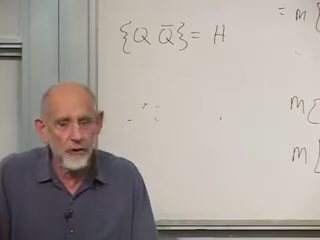
\includegraphics[width=0.62\textwidth]{lecture_05_figure_02.png}\lectureframe{00:55:46.300}\caption{칠판에 나타낸 중심 닫힘 관계. 괄호와 \(Q,\bar Q,H\)가 보이며, 쉼표는 표준 반교환자 표기법에 따라 보충했다.}\end{figure}

진공 에너지는 빈 상태의 에너지가 \(H=0\)가 되도록 정했다. 초대칭 조화진동자에서는 보손과 페르미온의 영점 에너지가 상쇄되므로 이것이 자연스러운 규약이다. \editorialnote{강의에서는 영점 에너지를 따로 표시하지 않고 총 정지 에너지로 직접 계산한다. 여기서 밝힌 규약은 그 선택을 명확히 한다.}

해밀토니안은 짝수다. 또한 대칭 생성자이기도 하다. 시간 병진을 생성하기 때문이다. 따라서 짝수인 시간 병진 생성자를 포함하지 않으면 홀수 생성자만으로 대수가 닫히지 않는다.

\begin{classroomqa}
\audiencequestion{이 관계에서 어떤 항이 짝수인가요? 해밀토니안인가요? \lecturetimestamp{00:58:24}}
\lecturerresponse{그렇다. 에너지는 보통의 관측가능량이므로 \(H\)는 짝수다. 초전하 \(Q\)는 홀수이고, 홀수 양 두 개의 곱은 짝수다. 따라서 \(\{Q,\bar Q\}\)가 \(H\)와 같을 수 있다. 홀수 생성자와 짝수 생성자 사이의 관계는 반교환자가 아니라 교환자로 주어진다.}
\end{classroomqa}

\subsection{대수를 완성하기}

같은 짝홀성의 원소 사이 관계는 자명하다.
\begin{equation}
\{Q,Q\}=2Q^2=0,
\qquad
\{\bar Q,\bar Q\}=2\bar Q^2=0,
\end{equation}
\(Q^2\)에 \(c_-^2\)가 들어 있고 \(\bar Q^2\)에 \(c_+^2\)가 들어 있기 때문이다.

남은 것은 \(H\)와의 관계다. 다음을 두자.
\begin{equation}
H\ket{E}=E\ket{E}.
\end{equation}
보손과 페르미온의 질량이 같으면 \(Q\)는 에너지를 바꾸지 않고 한 입자를 다른 입자로 바꾼다. 따라서 \(Q\ket{E}\)는 0이거나 같은 고유값을 갖는 또 다른 고유상태다.
\begin{equation}
H Q\ket{E}=E Q\ket{E}.
\end{equation}
한편
\begin{equation}
QH\ket{E}=Q(E\ket{E})=E Q\ket{E}.
\end{equation}
두 식을 빼면
\begin{equation}
[H,Q]\ket{E}=0.
\end{equation}
에너지 고유상태들이 완비 기저를 이룬다면, 이는 연산자 항등식으로 성립한다.
\begin{equation}
[H,Q]=0,
\qquad
[H,\bar Q]=0.
\end{equation}

\begin{classroomqa}
\audiencequestion{보손과 페르미온의 질량이 같지 않으면 어떻게 될까요? \lecturetimestamp{01:01:16}}
\lecturerresponse{그러면 한쪽을 다른 쪽으로 바꿀 때 에너지가 변하므로, 제안된 초전하는 해밀토니안과 교환하지 않고 단순한 초대칭은 사라집니다. 구체적으로,
\[
H=m_BN_B+m_FN_F,
\]
명시적인 계산 결과는 다음과 같습니다.
\[
[H,Q]=(m_B-m_F)Q.
\]
이 결과는 \(m_B=m_F\)일 때에만 정확히 0이 됩니다. \editorialnote{질량이 다를 때의 교환자는 에너지 변화 논증을 연산자 형태로 직접 나타내며, 질량이 같아야 한다는 조건을 명시적으로 보여 줍니다.}}
\end{classroomqa}

\begin{classroomqa}
\audiencequestion{에너지 고유상태를 이용한 논증을 좀 더 천천히 다시 설명해 주실 수 있나요? \lecturetimestamp{01:01:37}}
\lecturerresponse{\(H\ket{E}=E\ket{E}\)에서 시작합니다. 질량이 같으면 \(Q\ket{E}\)도 같은 확정 에너지 \(E\)를 가지므로 \(HQ\ket{E}=EQ\ket{E}\)입니다. 반대 순서로 연산하면 \(QH\ket{E}=QE\ket{E}=EQ\ket{E}\)가 됩니다. \(E\)은 보통의 스칼라량이기 때문입니다. 따라서 두 결과의 차이는 모든 에너지 고유상태에서 0입니다. 완비성을 이용하면 이 관계를 각 상태에 대한 명제에서 연산자 방정식 \([H,Q]=0\)으로 확장할 수 있습니다.}
\end{classroomqa}

따라서 모형의 대수 전체는 다음과 같다.
\begin{align}
\{Q,\bar Q\}&=H,\\
\{Q,Q\}&=\{\bar Q,\bar Q\}=0,\\
[H,Q]&=[H,\bar Q]=0.
\end{align}
초전하들은 보존되는 홀수 전하다. 더 놀라운 점은 이들의 대수가 입자 종류를 바꾸는 작용과 시공간 병진 생성자를 결합한다는 것이다.

\section{해밀토니안이 시간 병진을 뜻하는 이유}

이 단순화된 모형에는 공간 좌표는 없지만 시간은 있다. 슈뢰딩거 방정식은 다음과 같다.
\begin{equation}
i\frac{\partial}{\partial t}\ket{\psi(t)}
=H\ket{\psi(t)}.
\end{equation}

\begin{figure}[H]\centering
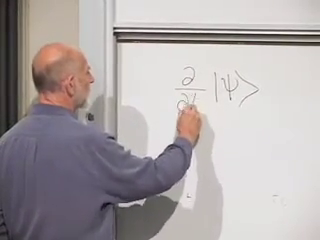
\includegraphics[width=0.56\textwidth]{lecture_05_figure_03.png}\lectureframe{01:07:26.300}\caption{\(\ket{\psi}\)의 시간 미분을 옆에 적고 있다. 손이 분모 일부를 가리고 있지만, 완전한 슈뢰딩거 방정식은 앞에 제시했다.}\end{figure}

유한한 시간 변화 \(\delta\)에 대해
\begin{equation}
\ket{\psi(t+\delta)}
=e^{-iH\delta}\ket{\psi(t)}.
\end{equation}
1차까지 전개하면
\begin{equation}
\ket{\psi(t+\delta)}
=\left(\mathbf 1-i\delta H\right)\ket{\psi(t)}
+O(\delta^2).
\end{equation}
따라서 \(H\)는 시간에 따라 상태를 변화시키는 무한소 생성자다.

아이소스핀이나 색과 같은 내부 대칭도 입자의 표지를 바꾼다. 아이소스핀은 양성자와 중성자 상태를 섞을 수 있고, 색 회전은 빨강, 초록, 파랑 쿼크를 서로 섞는다. 그러나 내부 변환을 아무리 조합해도 계를 공간이나 시간에서 병진시키지는 못한다. 초대칭은 다르다.
\begin{equation}
\begin{gathered}
\text{odd particle-changing transformation}\\
\mathrel{\stackrel{\{\ ,\ \}}{\Longrightarrow}}\\
\text{time translation}
\end{gathered}
\end{equation}
이 점은 홀수 생성자 자체가 보통 좌표와는 다른 좌표를 따른 병진일 수 있음을 시사한다.

\section{초공간}

\subsection{시간과 홀수 좌표의 함수}

다음 함수를 도입하자.
\begin{equation}
\Psi=\Psi(\theta,\bar\theta,t).
\end{equation}
모형에서는 파동함수로, 더 일반적으로는 초장으로 볼 수 있다. 홀수 변수에 대한 전개는 유한 항에서 끝나므로
\begin{equation}
\Psi(\theta,\bar\theta,t)
=A(t)+\bar\chi(t)\theta
+\bar\theta\chi(t)+F(t)\bar\theta\theta.
\end{equation}
하나의 대상에 짝수 성분 함수와 홀수 성분 함수가 함께 들어간다. \editorialnote{이 성분 전개는 앞에서 다룬 그래스만 다항식을 적용한 것이다. 초공간 위의 함수가 구체적으로 어떤 형태인지 표준적인 방식으로 나타낸다.}

보통의 시간 병진은 \(\theta,\bar\theta\)를 고정한 채 다음 변환을 한다.
\begin{equation}
t\longmapsto t+\delta.
\end{equation}
1차까지는
\begin{equation}
\Psi(\theta,\bar\theta,t+\delta)
=\Psi(\theta,\bar\theta,t)
+\delta\,\partial_t\Psi(\theta,\bar\theta,t).
\end{equation}

\begin{figure}[H]\centering
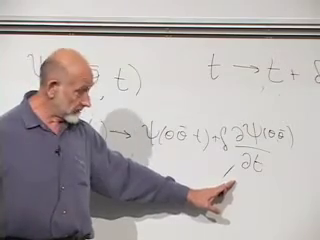
\includegraphics[width=0.72\textwidth]{lecture_05_figure_04.png}\lectureframe{01:13:15.060}\caption{첫 번째 차수에서 \(t\to t+\delta\)를 표시하고 그 아래에 \(\Psi\)의 변화량을 적었다. 미분 항도 바로 옆에 나타나 있다.}\end{figure}

\subsection{홀수 방향의 병진}

이제 홀수 좌표를 이동시키는 변환을 정의하자.
\begin{equation}
\theta\longmapsto\theta+\epsilon,
\end{equation}
여기서 \(\epsilon\)는 또 다른 홀수 그래스만 매개변수다. 이와 함께 시간에도 짝수 멱영 변위를 준다.
\begin{equation}
t\longmapsto t+i\bar\theta\epsilon.
\end{equation}
\(\bar\theta\)와 \(\epsilon\)는 둘 다 홀수이므로 그 곱은 짝수다. 따라서 짝수 좌표 \(t\)에 일관되게 더할 수 있다.

매개변수를 왼쪽으로 옮기면
\begin{equation}
i\bar\theta\epsilon=-i\epsilon\bar\theta.
\end{equation}
유도되는 변화량은 따라서
\begin{align}
\delta_\epsilon\Psi
&=\epsilon\,\partial_\theta\Psi
-i\epsilon\bar\theta\,\partial_t\Psi\\
&=\epsilon q_0\Psi,
\end{align}
이며, 여기서
\begin{equation}
q_0=\partial_\theta-i\bar\theta\partial_t.
\end{equation}
이다. 이 홀수 미분 연산자가 두 변위를 결합한 변환의 생성자다. 왼쪽 미분을 사용할 때 이에 맞는 켤레 생성자는 다음과 같다.
\begin{equation}
\bar q_0=-\partial_{\bar\theta}
+i\theta\partial_t.
\end{equation}

정확한 부호는 왼쪽 그래스만 미분과 오른쪽 그래스만 미분 중 어느 것을 사용하는지, 그리고 켤레화할 때 홀수 인자의 순서를 어떻게 뒤집는지에 따라 달라집니다. 어떤 규약을 사용하더라도 시간 병진으로의 닫힘은 변하지 않아야 합니다. 위에서 정의한 것을 사용하면,
\begin{align}
\{q_0,\bar q_0\}
&=i\{\partial_\theta,\theta\}\partial_t
+i\{\bar\theta,\partial_{\bar\theta}\}\partial_t\\
&=2i\partial_t.
\end{align}
미분 연산자끼리의 항은 사라지고 홀수 좌표에 대한 이차항도 사라집니다. 두 혼합항은 각각 \(i\partial_t\)를 줍니다.

슈뢰딩거 그림의 상태에서는 \(H=i\partial_t\)이므로
\begin{equation}
\{q_0,\bar q_0\}=2H.
\end{equation}
다음과 같이 정규화하면
\begin{equation}
q=\frac{q_0}{\sqrt2},
\qquad
\bar q=\frac{\bar q_0}{\sqrt2},
\end{equation}
다음을 얻는다.
\begin{equation}
\boxed{\{q,\bar q\}=H.}
\end{equation}
\editorialnote{강의에서는 부호가 확실하지 않은 상태로 계산을 진행한 뒤 계수 2가 생김을 확인한다. 위의 왼쪽 미분 규약은 강의의 계산을 유지하면서 일관된 정규화를 하나 정해 준다. 다른 표준 규약을 쓰면 부호가 좌표 변위와 생성자 사이에서 옮겨간다.}

\begin{classroomqa}
\audiencequestion{초공간 반교환자에 마지막 계수 2가 나타나는 이유는 무엇인가요? \lecturetimestamp{01:24:21}}
\lecturerresponse{같은 혼합 항이 두 개 있기 때문이다. 하나는 \(\{\partial_\theta,\theta\}=1\)에서, 다른 하나는 \(\{\partial_{\bar\theta},\bar\theta\}=1\)에서 나온다. 둘 다 시간 미분 항을 곱한다. 따라서 정규화하지 않은 생성자는 \(2i\partial_t\)를 주며, 각 초전하에 계수 \(1/\sqrt2\)를 곱하면 앞서 쓴 정규화가 복원된다.}
\end{classroomqa}

\begin{classroomqa}
\audiencequestion{\(\epsilon\)가 작다는 가정을 사용해 이 구성을 만들었나요? \lecturetimestamp{01:24:51}}
\lecturerresponse{보통의 수치적 크기가 아니라 멱영성을 이용했다. \(\epsilon^2=0\)이므로 \(\epsilon\)에 대한 모든 전개는 1차 항 뒤에서 끝난다. 무한소나 작은 양이라고 부르는 것은 유용한 비유지만, 전개가 끝나는 것은 정확한 결과다.}
\end{classroomqa}

\editorialnote{그래스만 매개변수에는 보통의 양의 크기가 없다. 이들이 무한소 매개변수 역할을 하는 까닭은 멱영성과 전개의 정확한 종료에 있다.}

\subsection{기하학적 의미}

이제 대수를 구현하는 서로 동등한 두 방식이 있다. 조화진동자 관점에서는 \(Q\)와 \(\bar Q\)가 페르미온을 보손으로, 보손을 페르미온으로 바꾼다. 기하학적 관점에서는 \(q\)와 \(\bar q\)가 홀수 방향으로 함수를 병진시키면서 보통의 시간 변위도 일으킨다. 두 관점 모두에서
\begin{equation}
\begin{gathered}
\{\text{supercharge},\text{conjugate supercharge}\}\\
=\text{time-translation generator}.
\end{gathered}
\end{equation}

\(t,\theta,\bar\theta\)를 포함하는 일반화된 좌표 공간이 초공간이다. 상대론적 장 이론에서는 여기에 보통의 공간 좌표도 포함되며, 초전하들은 \(H=P_0\)뿐 아니라 전체 시공간 운동량 \(P_\mu\)으로 닫힌다. 이 구조를 곡률이 있는 공간으로 확장하면 초중력으로 이어진다.

한편으로 그래스만 변수는 보손과 페르미온을 효율적으로 추적하는 도구다. 다른 한편으로 닫힘 관계는 훨씬 더 깊은 것을 말해 준다. 입자의 종류와 시공간 기하 사이의 구분은 더 이상 절대적이지 않다. 홀수 방향으로 두 번 이동하면 보통의 방향으로 움직이게 된다. 자연이 이 구조를 실험적으로 구현하는지는 별개의 문제다. 이 구조가 일관되고 간결하며 놀라울 만큼 엄격한 수학적 틀이라는 사실은 변하지 않는다.

\chapter{초대칭이 중요할 수 있는 이유}

\lectureoverview{이 장의 여러 주제는 진공 요동으로 연결된다.
경계 조건은 카시미르 힘을 만들고, 루프 효과는 힉스 질량을 위협하며, 새로운 가상 입자는 게이지 결합의 에너지에 따른 변화를 바꾸고, 진공 에너지는 우주의 팽창을 좌우한다. 이러한 문제들은 힉스 척도를 안정화하고 암흑물질 후보를 제공하며 게이지 결합의 통일을 개선하는 방법으로 저에너지 초대칭을 생각해 보게 한다. 이어서 그라스만 좌표를 사용해 초장을 구성하고, 베레진 적분으로 초대칭 작용을 구한다.}

\section{반사판 사이의 진공 요동}

카시미르 효과에 관한 질문을 먼저 정리하며 초대칭으로 돌아가 보자. 서로 \(d\)만큼 떨어진 평행한 반사판 두 개를 놓는다. 실제 입자가 하나도 없더라도 양자장은 진공 요동을 갖는다. 이를 가상 과정으로 그려 볼 수도 있고, 동등하게 장의 진동자 모드가 갖는 영점 운동으로 볼 수도 있다. 판은 경계 조건을 부과하므로, 판 사이에서 허용되는 요동은 제한 없는 공간에서의 요동과 달라진다.

중요한 것은 에너지의 절대적인 영점이 아니라 판 사이 거리가 변할 때 생기는 변화다. 단위 면적당 진공 에너지를 \(\mathcal E(d)=E(d)/A\)로 나타내자. \(\mathcal E\)가 \(d\)에 따라 달라지면 이는 퍼텐셜 에너지이며, 단위 면적당 힘은 다음과 같다.
\begin{equation}
\frac{F}{A}=-\frac{d\mathcal E}{dd}.
\end{equation}
따라서 가상 과정의 재배열은 관측 가능한 힘으로 나타난다. 이상적인 도체판을 예로 든 익숙한 전자기적 결과에서 에너지와 압력은 다음과 같다.
\begin{align}
\mathcal E(d)&=-\frac{\pi^2}{720\,d^3},\\
\frac{F}{A}&=-\frac{\pi^2}{240\,d^4},
\end{align}
단위는 \(\hbar=c=1\)이다.\editorialnote{이 계수들과 \(d^{-3}\)에 따른 면적당 에너지 및 \(d^{-4}\)에 따른 압력의 구분으로 칠판에서 제기된 차원에 관한 의문을 해소할 수 있다. 이는 여기서 유도하는 결과가 아니라, 이상적인 판에 대해 잘 알려진 표준 결과다.} 마이너스 부호는 인력을 뜻한다.

\begin{classroomqa}
\audiencequestion{네제곱에 반비례하는 것은 힘인가, 에너지인가? \lecturetimestamp{00:04:39}}
\lecturerresponse{시공간이 4차원일 때 평행판의 단위 면적당 에너지는 \(d^{-3}\)에 따라 감소하지만, \(d\)에 대해 미분하면 단위 면적당 힘은 \(d^{-4}\)에 따라 감소한다. \(\hbar\)와 \(c\)를 다시 넣으면 차원 분석만으로도 이 거듭제곱을 정할 수 있다.}
\end{classroomqa}

계산을 판이 가상 광자 루프를 끊는 과정이라고 요약하기도 한다. 이 그림은 지나치게 문자 그대로 받아들이지 않는다면 유용하다. 정확한 계산은 허용되는 장 모드의 스펙트럼 변화, 또는 동등하게 양자 유효 작용의 변화다. 어느 쪽으로 설명하든 거리 의존적인 에너지는 같다.

\begin{classroomqa}
\audiencequestion{카시미르 힘은 인력이 아니라 척력일 수도 있나요? \lecturetimestamp{00:07:48}}
\lecturerresponse{그럴 수 있다. 부호는 보편적으로 정해져 있지 않고 장, 기하학적 구조, 재료, 경계 조건에 따라 달라진다. 페르미온 루프는 보손 루프와 반대되는 루프 부호를 갖는 경우가 많아 칠판에서 나온 제안의 동기가 되지만, 페르미온 통계만으로 모든 카시미르 힘이 척력이어야 한다는 일반 정리가 성립하는 것은 아니다.\editorialnote{이 단서는 잠정적으로 제시했던 수업 중 답변을, 잘못된 보편 법칙을 피하는 데 필요한 일반적인 진술로 다듬는다.}}
\end{classroomqa}

\subsection{진공 에너지의 증거로 무엇을 들 수 있을까?}

카시미르 힘은 측정되며, 원자 관측량도 진공 루프에 민감하다. 그러나 이 사실들만으로는 진공의 절대 에너지가 중력에 기여한다는 점이 입증되지 않는다. 카시미르 실험은 경계로 인해 생기는 에너지 차이를 측정한다. 절대 영점 에너지를 발산하는 합에 조작적 의미를 부여하지 않고도 같은 힘을 설명할 수 있다.

결정적인 검증은 중력에서 나온다. 에너지는 중력 전하다. 빈 공간에 균일한 에너지 밀도가 있다면 아인슈타인 방정식에 들어가 우주의 팽창에 영향을 주어야 한다. 따라서 우주의 가속 팽창은 진공과 비슷한 성분에 대한 직접적인 중력 증거다.

\begin{classroomqa}
\audiencequestion{물리학자들이 진공 에너지가 무엇인지 모르는 것처럼, 대중 매체에서는 왜 진공 에너지를 수수께끼라고 부르나요? \lecturetimestamp{00:08:19}}
\lecturerresponse{양자장론에서는 모든 장에 영점 기여가 있으므로 진공 에너지가 존재할 가능성 자체는 수수께끼가 아니다. 수수께끼는 그 양에 있다. 알려진 양자장과 고에너지 컷오프를 바탕으로 한 추정값에 비해, 중력에 기여하는 값이 왜 그토록 극도로 작은가? 놀라운 것은 진공 에너지의 존재 자체가 아니라 그것이 거의 없다는 점이다.}
\end{classroomqa}

오랫동안 관측으로 정해진 상한은 매우 작아서, 우주상수를 정확히 영으로 놓고 상쇄를 강제하는 원리를 찾고 싶은 심리적 유혹이 있었다. 그러나 우주론 관측이 정밀해지면서 작지만 0이 아닌 값이 발견되었다. 이 발견으로 진공 에너지가 개념적으로 낯선 것이 된 것은 아니었다. 설명되지 않은 억제의 정도를 더는 외면할 수 없게 된 것이다. 관련된 비교는 가정하는 자외선 척도에 따라 달라지지만, 자연스러운 고에너지 추정은 모두 엄청난 상쇄를 요구한다.

\section{초전하 하나가 다입자 상태에 작용하면}

초대칭을 지지하는 이유를 열거하기 전에, 먼저 한 가지 역설처럼 보이는 문제를 풀어야 한다. 보손은 하나의 모드에 임의로 많은 수가 들어갈 수 있지만, 페르미온 모드의 점유수는 0 또는 1이다. 보손과 페르미온을 서로 바꾸는 대칭이 있다면, 한 모드에 있는 보손 천 개를 같은 모드에서 금지된 페르미온 천 개로 바꾸는 것일까?

아니다. 페르미온 생성자는 한 번에 양자 하나를 바꾼다. 진동자 모형에서 \(a\)가 보손을 소멸시키고 \(c^\dagger\)가 그 짝인 페르미온을 생성하게 하자. 초전하 하나는 다음과 같이 나타낼 수 있다.
\begin{equation}
Q=c^\dagger a.
\end{equation}
보손이 \(n\)개 있고 페르미온은 없는 상태에 작용시키면,
\begin{equation}
Q\ket{n,0}
=\sqrt n\,\ket{n-1,1}.
\end{equation}
보손 하나가 제거되고 페르미온 하나가 들어간다. 같은 전하를 다시 작용시키면 결과는 0이다.
\begin{equation}
Q^2=(c^\dagger)^2a^2=0.
\end{equation}
이는 페르미온 생성 연산자에서 물려받은 멱등성이다.

\begin{classroomqa}
\audiencequestion{많은 보손이 같은 상태를 차지하고 있다면, 초대칭 변환은 왜 그 상태에 있는 보손들을 다수의 페르미온으로 바꾸어 배타 원리를 위반하게 만들지 않을까? \lecturetimestamp{00:12:05}}
\lecturerresponse{생성자는 전체 점유 상태를 통째로 바꾸지 않는다. 페르미온 수를 한 단위만큼 바꾼다. 같은 페르미온 전하는 보통의 회전 생성자처럼 거듭 합성할 수 없는데, 그 제곱이 사라지기 때문이다. 이에 대응하는 전하를 작용시키면 그 교환을 되돌릴 수 있고, 혼합 반교환자는 시간 병진으로 닫힌다.}
\end{classroomqa}

마지막 문장은 핵심이다. 약식 표기 \(Q^2=0\)는 개별 카이랄 성분이나 방금 쓴 단순한 전하에 적용된다. 모든 초전하의 곱이 사라진다는 뜻은 아니다. 네 차원 초대칭에서,
\begin{equation}
\{Q_\alpha,\bar Q_{\dot\beta}\}
=2\sigma^\mu_{\alpha\dot\beta}P_\mu,
\end{equation}
한편 중심 전하가 없는 최소 대수에서는
\begin{equation}
\{Q_\alpha,Q_\beta\}=0,
\qquad
\{\bar Q_{\dot\alpha},\bar Q_{\dot\beta}\}=0
\end{equation}
가 성립한다.\editorialnote{이 성분 표현은 같은 \(Q\)를 거듭 작용시키면 사라지는 반면, 초전하와 그 켤레가 함께 병진을 생성한다는 강의실식 약식 설명을 정확히 나타낸다.}

\section{저에너지 초대칭을 탐색할 세 가지 이유}

\begin{classroomqa}
\audiencequestion{진공 에너지 상쇄 말고도 초대칭을 뒷받침하는 동기가 있나요? \lecturetimestamp{00:15:06}}
\lecturerresponse{서로 긴밀히 관련된 동기는 세 가지다. 힉스 자기 에너지의 제어, 안정한 암흑물질 입자 후보, 그리고 고에너지에서 게이지 결합이 훨씬 더 정확히 만난다는 점이다. 어느 하나도 자연계에서 초대칭이 실현된다는 것을 증명하지는 않지만, 세 가지를 함께 보면 초대칭은 진지하게 검증할 가치가 있는 이론이다.}
\end{classroomqa}

\emph{저에너지 초대칭}이라는 말은 상대적인 표현이다. 초짝입자의 질량이 일상적인 척도에서 가볍다는 뜻이 아니라, 질량이 전약 척도와 가속기 척도보다 엄청나게 높지는 않다는 뜻이다. 초짝입자의 질량이 한없이 높아지면 세 가지 논거 모두 약해진다.

\subsection{힉스 척도 보호하기}

스칼라 질량은 고에너지 물리에 유별나게 민감하다. 개략적으로 보손 루프는 다음 형태의 보정을 만든다.
\begin{equation}
\delta m_H^2\big|_{\mathrm B}
\sim +\frac{\lambda}{16\pi^2}\Lambda^2,
\end{equation}
여기서 \(\Lambda\)는 유효 이론을 적용하는 에너지 척도를 나타낸다. 페르미온 루프는 반대 부호를 갖는다.
\begin{equation}
\delta m_H^2\big|_{\mathrm F}
\sim -\frac{|y|^2}{8\pi^2}\Lambda^2.
\end{equation}
계수는 상호작용과 장의 중복도에 따라 달라지지만, 초대칭은 계수들을 서로 연관시켜 초짝 사이에서 선도 자외선 민감도가 상쇄되도록 한다.\editorialnote{이 개략적인 루프 식은 자기 에너지에 관한 정성적 논거의 바탕이 되는 수학을 보여 준다. 표준모형의 힉스 질량을 완전히 계산하려는 식은 아니다.}

힉스의 진공 기댓값이 전약 척도를 정하므로 이 점이 중요하다. 게이지 보손과 페르미온의 질량은 다음과 같은 관계를 따른다.
\begin{equation}
m_W=\frac{gv}{2},
\qquad
m_f=\frac{y_fv}{\sqrt2}.
\end{equation}
힉스 부문이 자연스럽게 엄청난 척도로 밀려난다면, 익숙한 저에너지 입자 스펙트럼은 사라질 것이다. 이를 유지하려면 복사 보정과 맨질량 매개변수를 극도로 정밀하게 맞춰야 한다.

정확한 초대칭이라면 상쇄도 정확하겠지만, 관측된 보손과 페르미온의 질량이 서로 다르므로 정확한 초대칭은 이미 배제되어 있다. 연성 깨짐 초대칭에서는 이차 민감도가 초짝 질량 분할에 대한 의존성으로 대체된다. 개략적으로
\begin{equation}
\delta m_H^2
\sim
\frac{g^2}{16\pi^2}
\left(m_{\mathrm{soft}}^2-m_{\mathrm{ordinary}}^2\right)
\ln\frac{\Lambda^2}{m_{\mathrm{soft}}^2}.
\end{equation}
질량 분할이 너무 크지 않을 때에만 상쇄가 유용하게 유지된다.

\subsection{암흑물질 붕괴 연쇄의 안정한 종착점}

스펙트럼을 보통 입자와 초짝입자로 나누어 보자. 페르미온에는 보손 초짝이 있고, 보손에는 페르미온 초짝이 있다. 두 부류를 구분하는 패리티를 상호작용이 보존한다면, 초짝입자가 붕괴할 때 다른 초짝입자가 남아야 한다.
\begin{equation}
\widetilde X
\longrightarrow X+\widetilde Y
\longrightarrow X+Y+\widetilde Z
\longrightarrow\cdots.
\end{equation}
붕괴 연쇄에서 마지막 초짝입자를 없앨 수는 없다. 따라서 연쇄는 가장 가벼운 초대칭 입자인 LSP에서 끝난다.

널리 쓰이는 대칭은 \(R\)-패리티다.
\begin{equation}
R_p=(-1)^{3(B-L)+2s}.
\end{equation}
표준모형 입자는 \(R_p=+1\)이고, 초짝입자는 \(R_p=-1\)이다. \(R_p\)가 정확히 보존되면 모든 상호작용에는 초짝입자가 짝수 개 포함되며 LSP는 안정하다.\editorialnote{초대칭만으로 안정한 LSP가 보장되지는 않는다. 안정하려면 \(R\)-패리티나 같은 결과를 낳는 다른 대칭이 보존되어야 한다. 그렇지 않으면 LSP는 붕괴할 수 있다.}

암흑물질은 우주론적 시간 척도보다 오래 살아남아야 한다. 또한 눈에 보이는 은하 원반을 반복해서 지나가도 에너지를 상당량 잃지 않을 만큼 약하게 상호작용해야 한다. 전하를 띠거나 강하게 상호작용하는 입자 집단은 산란하고 에너지를 소산하여 보통 물질과 같은 얇은 구조로 모이는 경향이 있다. 관측된 넓은 헤일로는 대신 전기적으로 중성이며 약하게 상호작용하는 성분을 시사한다.

그렇다고 LSP가 무엇인지 유일하게 정해지는 것은 아니다. 모형과 대칭 깨짐 양상에 따라 후보는 전약 게이지노와 힉시노가 섞인 중성 입자일 수도 있고, 그래비티노일 수도 있다. 전하를 띠거나 색전하를 가진 후보는 강한 제약을 받는다. 초대칭이 제공하는 것은 보장된 답이 아니라 중성이며 오래 살아남는 종착점을 만들어 내는 자연스러운 메커니즘이다.

\section{에너지에 따른 결합의 변화와 통일의 단서}

세 번째 동기는 전하 차폐에서 출발한다. 가상 입자가 상호작용을 둘러싸므로 측정되는 결합은 에너지 척도에 따라 달라진다. 전자기학에서는 광자 전파자에 삽입된 전자-양전자 루프가 먼 거리에서 전하를 차폐한다. 더 짧은 거리, 즉 더 높은 운동량 전달에서는 탐침 사이에 놓인 분극 구름의 양이 줄어 유효 전하가 커진다.

다음과 같이 쓰자.
\begin{equation}
\alpha_i=\frac{g_i^2}{4\pi}.
\end{equation}
1루프 근사에서 역결합은 에너지의 로그에 따라 선형으로 변한다.
\begin{equation}
\frac{d\alpha_i^{-1}}{d\ln\mu}
=-\frac{b_i}{2\pi}.
\end{equation}
따라서
\begin{equation}
\alpha_i^{-1}(\mu)
=\alpha_i^{-1}(\mu_0)
-\frac{b_i}{2\pi}\ln\frac{\mu}{\mu_0}.
\end{equation}
\editorialnote{이 1루프 방정식은 로그 에너지를 가로축으로 그렸을 때 거의 직선인 그래프의 정확한 표현이다. 문턱 효과와 고차 루프 보정으로 직선은 조금 휘어진다.}

전약 척도 위에서 기본 게이지 결합 세 가지는 다음 게이지 군에 해당한다.
\begin{equation}
U(1)_Y,\qquad SU(2)_L,\qquad SU(3)_c.
\end{equation}
저에너지에서 직관을 위해 사용하는 전자기 결합은 전약 대칭 깨짐 뒤 첫 번째와 두 번째 결합의 조합이다. QCD에서는 비가환 게이지장이 반차폐를 일으킨다. 이것이 짧은 거리에서 강한 결합이 약해지는 점근적 자유 현상이다. 따라서 \(\alpha_3^{-1}\)은 \(\ln\mu\)에 따라 증가하는 반면, 나머지 역결합은 기울기가 다르다.

표준모형 곡선은 서로 가까워지는 듯 보이지만 한 점에서 만나지는 않는다. 초짝입자는 가상 루프를 바꾸고, 따라서 계수 \(b_i\)를 바꾼다. 통상적인 대통일 정규화에서
\begin{align}
(b_1,b_2,b_3)_{\mathrm{SM}}
&=\left(\frac{41}{10},-\frac{19}{6},-7\right),\\
(b_1,b_2,b_3)_{\mathrm{MSSM}}
&=\left(\frac{33}{5},1,-3\right).
\end{align}
초짝입자 문턱이 TeV 척도 부근에 있으면, 외삽한 초대칭 곡선은 다음 부근에서 훨씬 정확하게 만난다.
\begin{equation}
M_{\mathrm{GUT}}\sim 10^{16}\ \mathrm{GeV}.
\end{equation}
어떤 실험도 이 척도에 직접 도달하지 못한다. 저에너지 결합을 측정하고, 장의 구성으로 에너지에 따른 변화를 정한 다음, 여러 자릿수에 걸쳐 곡선을 외삽한다. 두 직선은 언제나 어딘가에서 교차한다. 서로 독립적인 세 직선이 한 점 부근에서 만난다는 것이 의미 있는 관측이다.

\begin{classroomqa}
\audiencequestion{개선된 외삽은 정확한 초대칭과 초짝입자의 동일한 질량을 가정하나요? \lecturetimestamp{00:38:09}}
\lecturerresponse{아니다. 초대칭은 깨져 있으므로 질량에 분할이 생긴다. 중요한 것은 초짝입자 루프가 에너지에 따른 변화에 언제부터 들어오는가이다. 초짝입자가 지나치게 무겁지 않다면 세 결합의 기울기가 충분히 이른 시기에 바뀌어 서로 수렴한다. 초짝입자가 극도로 무거우면 초대칭 문턱이 너무 늦게 나타나 개선된 수렴이 사라진다.}
\end{classroomqa}

문턱 보정과 미지의 고에너지 스펙트럼 때문에 세 직선이 수학적으로 정확히 한 점에서 만난다고 단정할 수는 없다. 그래도 결과는 놀랍다. 힉스 문제를 완화하고 열적 암흑물질 후보를 제공하는 바로 그 근사적인 초짝입자 척도가 통일도 개선한다.

\subsection{중력과 공통의 고에너지 척도}

중력은 전하가 에너지 자체라는 점에서 다르게 작용한다. 질량중심 에너지 \(E\)에서 유용한 무차원 척도는 다음과 같다.
\begin{equation}
\alpha_G(E)\sim GE^2
=\left(\frac{E}{M_{\mathrm{Pl}}}\right)^2.
\end{equation}
일상적인 에너지에서는 이 값이 믿기 어려울 만큼 작지만, \(E\)의 제곱에 비례해 증가한다. 따라서 그 역수는 로그에 따라 변하는 게이지 역결합보다 훨씬 빠르게 감소하여 플랑크 척도 부근에서 1 정도가 된다.

이 비교는 모든 상호작용이 서로 가까운 높은 에너지 척도에서 지배될 가능성을 시사하지만, 게이지 통일보다는 덜 명확하다. 게이지 결합은 재규격화 가능한 장론의 무차원 매개변수인 반면, 뉴턴 상수는 차원을 가지므로 중력을 같은 그래프에 나타내려면 규약을 정해야 한다.

\begin{classroomqa}
\audiencequestion{초짝입자는 같은 세 게이지 상호작용에 참여하나요, 아니면 새로운 힘을 정의하나요? \lecturetimestamp{00:42:35}}
\lecturerresponse{초짝입자는 짝이 되는 입자와 같은 게이지 양자수를 가진다. 셀렉트론은 전자와 같은 전하를 띠고, 스쿼크는 스핀과 질량은 다르지만 해당 쿼크와 같은 색전하 및 전약 전하를 가진다. 따라서 초짝입자의 루프는 새로운 게이지 상호작용 세 가지를 도입하는 것이 아니라 기존의 같은 게이지 상호작용을 바꾼다.}
\end{classroomqa}

\begin{classroomqa}
\audiencequestion{LHC에서 초짝입자를 발견하면 초대칭의 결정적 증거가 되나요? \lecturetimestamp{00:43:27}}
\lecturerresponse{낯선 입자 하나만 발견하고 그 이름을 붙이는 것으로는 충분하지 않다. 그러나 스핀, 전하, 질량, 결합 사이의 초대칭 관계를 따르는 초짝입자 스펙트럼은 매우 뚜렷한 특징을 보일 것이다. 초대칭은 서로 연관된 여러 제약을 부과하므로, 구체적인 상호작용 양상이 결정적인 검증이 된다.}
\end{classroomqa}

\subsection{척도를 높이면 대가를 치르는 이유}

초짝입자의 질량이 실험으로 도달할 수 있는 범위를 조금 넘어서는 정도라면 세 가지 동기는 여전히 작동할 수 있다. 질량을 여러 자릿수만큼 높이면 각각의 논거가 약해진다.
\begin{enumerate}\item 힉스 질량의 상쇄 뒤에도 질량 분할에 대한 큰 잔여 민감도가 남는다.
\item 통상적인 약한 척도의 열적 잔존 입자가 예상한 척도에서 더는 생기지 않는다.
\item 게이지 결합의 에너지에 따른 변화에서 문턱이 더 높은 에너지로 밀려 세 결합의 수렴이 덜 정확해진다.
\end{enumerate}
초대칭은 훨씬 높은 척도에서 여전히 존재할 수 있지만, 그런 경우에는 이 특정한 저에너지 문제들을 그만큼 경제적인 방식으로 해결하지 못한다. 이 아이디어가 오래 이어졌다고 해서 자연이 반드시 이를 따른다는 증거가 되는 것은 아니다. 다만 결정적인 검증을 받을 만큼 일관성 있는 제안이라는 뜻이다.

\section{암흑물질에 관해 우주론으로 알 수 있는 것과 알 수 없는 것}

\begin{classroomqa}
\audiencequestion{핵합성으로 수소와 헬륨을 제한하듯, 표준 우주론으로 암흑물질의 양과 암흑물질 입자 하나의 질량을 알아낼 수 있나요? \lecturetimestamp{00:46:32}}
\lecturerresponse{우주론은 암흑물질의 총 질량 밀도를 매우 정확히 측정하지만, 밀도만으로는 질량과 개수를 구분할 수 없다. 같은 밀도를 무거운 입자 몇 개가 만들 수도 있고, 매우 가벼운 입자가 엄청나게 많이 만들어 낼 수도 있다. 미시적 입자를 규명하려면 추가 이론이나 중력 이외의 관측이 필요하다.}
\end{classroomqa}

이러한 모호함을 보여 주는 두 가지 대표적인 가능성이 있다. 전약 척도 또는 TeV 척도 부근의 약하게 상호작용하는 입자는 뜨거운 열적 열평형계에서 동결 이탈할 수 있다. 반대편 극단에서는 액시온과 같은 매우 가벼운 보손이 결맞은 장 배치나 응축 상태를 이룰 수 있다. 가장 잘 발달한 두 메커니즘이 양극단 부근에 있다고 해서 그 사이의 가능성이 금지되는 것은 아니다.

헤일로의 구조 자체도 중요한 제약을 준다. 암흑물질은 보통 물질을 거의 마찰 없이 지나가므로 빛나는 원반으로 붕괴하지 않고 공간적으로 넓게 퍼진 채 남는다. 회전 곡선과 다른 중력 현상으로 질량이 존재한다는 사실은 알 수 있지만, 그 현상만으로 입자의 개수를 셀 수는 없다.

\begin{classroomqa}
\audiencequestion{초기 우주에는 초입자만 있다가 나중에 붕괴하여 지금 보이는 입자가 되었을 수도 있나요? \lecturetimestamp{00:49:11}}
\lecturerresponse{모든 관련 질량보다 훨씬 높은 온도에서는 빠른 반응으로 종들이 임의로 한쪽에 치우친 분포가 아니라 열평형에 가까워진다. 수가 부족한 초짝입자는 보통 입자들의 충돌로 생성되고, 초짝입자들의 충돌과 붕괴는 보통 입자를 다시 보충한다. 정확한 풍부도는 상호작용과 자유도에 따라 달라지지만, 뜨거운 플라스마는 계속 균형을 이루는 쪽으로 나아간다.}
\end{classroomqa}

우주가 식으면 무거운 종의 수는 볼츠만 억제로 줄고, 이들은 소멸하거나 붕괴한다. 안정한 LSP는 상호작용률이 우주 팽창보다 느려지면 열평형 상태를 더 이상 따라가지 않는다.
\begin{equation}
\Gamma_{\mathrm{ann}}
\sim n\langle\sigma v\rangle
\lesssim H.
\end{equation}
남은 입자들이 잔존 풍부도를 이룬다.\editorialnote{이 동결 이탈 조건은 열적 균형에 관한 설명을 정량적으로 마무리해 주는 표준 결과다. 특히 상호작용이 매우 약한 그래비티노를 비롯한 다른 LSP 후보는 비열적 이력을 가질 수 있다.}

\begin{classroomqa}
\audiencequestion{LSP는 어떤 보통 입자의 초짝이며, 반드시 상호작용하지 않아야 하나요? \lecturetimestamp{00:51:05}}
\lecturerresponse{모형에 무관한 답은 없다. 암흑물질 후보가 될 만한 LSP는 전기적으로 중성이며 색전하가 없을 것으로 예상되지만, 완전히 상호작용하지 않아야 하는 것은 아니다. 광자, 약한 게이지 보손, 힉스 장과 연관된 혼합 상태일 수도 있고, 그래비티노일 수도 있다. 정확한 정체는 초대칭 깨짐 스펙트럼에 따라 정해진다.}
\end{classroomqa}

\section{진공 다이어그램, 자기 에너지 다이어그램, 그리고 팽창}

\begin{classroomqa}
\audiencequestion{힉스 발산과 진공 에너지 발산은 어떻게 다른가요? \lecturetimestamp{00:52:09}}
\lecturerresponse{진공 다이어그램에는 외부 입자선이 없다. 이 다이어그램은 빈 공간의 유효 작용을 바꾸어 진공 에너지에 기여한다. 힉스 자기 에너지 다이어그램에는 외부 힉스 다리가 두 개 있다. 이 다이어그램은 힉스 전파자를 바꾸어 질량에 영향을 준다. 둘 다 가상 요동을 포함하지만, 서로 다른 질문에 답한다.}
\end{classroomqa}

실제 입자를 진공 속에 끼워 넣은 불순물로 생각해 볼 수 있다. 이 불순물에 붙는 진공 요동은 입자의 전파와 질량을 바꾼다. 카시미르 판도 진공 요동을 바꾸지만, 거시적인 경계 조건을 통해서다. 두 경우에 공통으로 작용하는 것은 끼워 넣은 대상에 대한 양자 요동의 반응이다. 보정되는 관측량은 경우마다 다르다.

\vspace{-2pt}\subsection{물질, 복사, 진공 에너지는 서로 다르게 희석된다}

\(a(t)\)를 우주론적 척도 인자라고 하고,
\begin{equation}
H=\frac{\dot a}{a}
\end{equation}
허블 매개변수를 다음과 같이 정의하자. 균일한 우주에서 국소적인 응력-에너지 보존은 다음을 준다.
\begin{equation}
\dot\rho+3H(\rho+p)=0.
\end{equation}
상태방정식이 \(p=w\rho\)이면 이를 적분하여 다음을 얻는다.
\begin{equation}
\rho(a)\propto a^{-3(1+w)}.
\end{equation}
\editorialnote{연속 방정식은 입자 수와 파장 늘어남으로 희석을 설명하는 간결한 유도 과정을 제공한다.}

차갑고 비상대론적인 물질에서는 \(p\approx0\)이므로,
\begin{equation}
\rho_m\propto a^{-3}.
\end{equation}
공변 부피가 \(a^3\)만큼 커지는 동안 그 안의 입자들이 가진 정지 에너지는 대략 일정하게 유지된다.

복사에서는 \(p=\rho/3\)이고,
\begin{equation}
\rho_r\propto a^{-4}.
\end{equation}
세 제곱만큼의 감소는 수 밀도의 희석에서 온다. 네 번째 제곱은 적색편이 때문이다.
\begin{equation}
\lambda\propto a,
\qquad
E_\gamma=\frac{2\pi\hbar c}{\lambda}\propto a^{-1}.
\end{equation}

\begin{classroomqa}
\audiencequestion{광자에게 파동함수가 있다면, 희석 법칙을 유도할 때 왜 파동이 아니라 입자로 말해도 되나요? \lecturetimestamp{00:58:21}}
\lecturerresponse{두 설명의 차이는 스케일링에 영향을 주지 않는다. 입자 관점에서는 공변 부피 안의 입자 수가 일정하고 각 양자의 에너지가 적색편이로 \(a^{-1}\)만큼 변한다. 고전적 파동 관점에서는 파장이 늘어나고 장의 에너지도 같은 비율로 감소한다. 우주 팽창을 이해하기 쉬운 쪽의 설명을 사용하면 된다.}
\end{classroomqa}

진공 에너지는 \(p_\Lambda=-\rho_\Lambda\)이므로,
\begin{equation}
\rho_\Lambda=\text{constant}.
\end{equation}
공간이 팽창해도 희석되지 않는다. 실제로 공변 영역 안의 에너지는
\begin{equation}
E_\Lambda=\rho_\Lambda a^3V_0,
\end{equation}
이며, 이 값은 물리적 부피와 함께 증가한다. 이 사실에서 생기는 에너지 보존의 문제를 잠시 뒤에 다루겠다.

이처럼 서로 다른 거듭제곱은 우주의 역사를 정리해 준다. 복사는 가장 빠르게 감소하고, 물질은 더 느리게 감소하며, 진공 에너지는 전혀 감소하지 않는다. 따라서 아주 작은 진공 항도 초기 우주에서는 무시할 수 있다가 후기에는 우주를 지배할 수 있다. 여기서 논의한 대략적인 값을 사용하면 현재의 에너지 예산은 진공 에너지가 약 \(70\%\), 물질이 \(30\%\)이며, 복사는 그보다 훨씬 적다.

\section{기하학은 에너지다}

아인슈타인 방정식의 시간-시간 성분은 앞서 살펴본 스케일링 법칙을 동역학으로 바꾼다. 칠판에는 표어와 하나의 기하학적 항이 적혀 있다.

\begin{figure}[H]
\centering
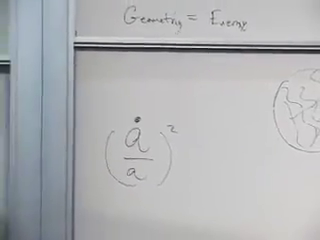
\includegraphics[width=0.68\textwidth]{lecture_06_figure_03.png}
\lectureframe{01:06:37.088}
\caption{팽창 항 \(H^2=(\dot a/a)^2\)을 그 아래에 적은, 핵심 표어 \emph{기하학은 에너지다}.}
\end{figure}

균일하고 등방적인 우주에서 제1 프리드만 방정식은 다음과 같다.
\begin{equation}
H^2+\frac{k}{a^2}
=\frac{8\pi G}{3}\rho,
\end{equation}
단위는 \(c=1\)이며, \(k=+1,0,-1\)는 닫힌 공간, 평탄한 공간, 열린 공간의 기하학을 나타낸다. 또한
\begin{equation}
\rho
=\rho_{\mathrm{ordinary}}
+\rho_{\mathrm{dark}}
+\rho_{\mathrm{radiation}}
+\rho_{\mathrm{vacuum}}.
\end{equation}
칠판에서 \(1/a^2\) 옆에 보이는 부호는 곡률 항을 좌변에 둘지 우변으로 옮길지, 그리고 \(k\)의 값이 무엇인지에 따라 달라진다.

\begin{figure}[H]
\centering
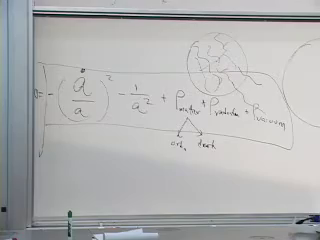
\includegraphics[width=0.96\textwidth]{lecture_06_figure_04.png}
\lectureframe{01:08:46.794}
\caption{칠판에 적힌 전체적인 균형식. 기하학 쪽에는 팽창과 공간 곡률이 있고, 원천 쪽에는 물질, 복사, 진공 에너지가 있다. 물질은 다시 보통 물질과 암흑 물질로 나뉜다.}
\end{figure}

\subsection{우주론적 해밀토니안 제약 조건}

\begin{classroomqa}
\audiencequestion{공동이동 영역 안의 진공 에너지가 우주 팽창에 따라 증가한다면, 일정한 순 에너지 밀도가 있는 것일까, 아니면 보존되는 총에너지가 있는 것일까? \lecturetimestamp{01:01:51}}
\lecturerresponse{일반 상대성 이론은 임의의 팽창 시공간에 대해 보편적인 전역 에너지를 제공하지 않는다. 그러나 균질한 우주론적 축약에서는 아인슈타인 방정식의 시간-시간 성분이 해밀토니안 제약식이다. 기하와 물질을 한쪽에 놓으면 제약된 해밀토니안은 0이 된다. 변하는 물질 항은 상자 안의 보통의 고정된 에너지가 아니라 중력 자유도에 의해 균형을 이룬다.}
\end{classroomqa}

개략적으로 쓰면 정준 관계는
\begin{equation}
\mathcal H_{\mathrm{gravity}}
+\mathcal H_{\mathrm{matter}}
=0.
\end{equation}
총에너지가 0이라고 말할 때의 정확한 의미가 이것이다. 이는 시간 재매개화 불변성이 강제하는 운동방정식이지, 모든 국소 에너지 밀도가 사라진다는 주장이 아니다. 공변 부피에서 보통 물질의 에너지는 대략 일정하고 복사 에너지는 감소하며 진공 에너지는 증가한다. 한편 중력 기여분과 팽창률은 아인슈타인 제약식이 계속 성립하도록 조정된다.

국소 보존은 여전히 정확히 성립한다:
\begin{equation}
\nabla_\mu T^{\mu\nu}=0.
\end{equation}
균일한 유체의 경우 이는 바로 연속 방정식이다.
\(\dot\rho+3H(\rho+p)=0\). 일반적으로 성립하지 않는 것은, 팽창하는 우주에서도 민코프스키 시공간에서의 직관처럼 좌표계에 무관한 전역적인 물질 에너지 총량 하나가 보존되어야 한다는 생각이다.\editorialnote{이러한 구분을 통해 에너지는 항상 0이라는 수업 중 설명을 정확히 이해할 수 있다. 국소 공변 보존 법칙과 우주론적 해밀토니안 제약식은 정확히 성립하지만, 물질과 중력을 합한 유일한 전역 에너지는 일반적으로 정의되지 않는다.}

\begin{classroomqa}\audiencequestion{에너지 제약식이 우주가 열린 우주인지, 닫힌 우주인지, 평탄한 우주인지를 결정하는 조건인가요? \lecturetimestamp{01:04:42}}\lecturerresponse{아니다. 해밀토니안 제약식은 모든 경우에 적용된다. 열린 우주, 평탄한 우주, 닫힌 우주는 곡률 표지 \(k\)에 따라, 따라서 \(k/a^2\) 항에 따라 서로 다르다. 곡률은 에너지 균형에서 한 기여 항을 바꾸지만, 제약식의 적용 여부를 바꾸지는 않는다.}\end{classroomqa}

\section{그라스만 좌표와 초장}

\begin{classroomqa}\audiencequestion{그라스만 수는 실제로 이론의 라그랑지안에 등장하나요? \lecturetimestamp{01:09:37}}\lecturerresponse{먼저 페르미온 장이 그라스만 홀수이기 때문에 등장한다. 또 초공간의 좌표로도 등장한다. 초장은 이 홀수 좌표에 의존하며, 초대칭 작용은 이 좌표에 관해 미분하고 적분하여 구성한다.}\end{classroomqa}

보통 장은 시공간의 함수다.
\begin{equation}
\phi=\phi(x^\mu).
\end{equation}
4차원 최소 초대칭에서는 \(x^\mu\)에 두 성분 홀수 스피너 \(\theta^\alpha\)와 그 켤레 \(\bar\theta^{\dot\alpha}\)를 더한다:
\begin{equation}
z^M=(x^\mu,\theta^\alpha,\bar\theta^{\dot\alpha}).
\end{equation}
복소 홀수 성분은 둘이며, 실수 홀수 방향은 넷이다. 초장은 이 초공간 위의 함수다:
\begin{equation}
\Phi=\Phi(x,\theta,\bar\theta).
\end{equation}

이것들은 계량의 의미에서 작은 공간 차원이 아니다. 그라스만 좌표에는 양의 수치적 크기가 없다. 그것이 작다고 부르는 것은 멱영성을 기억하기 위한 표현이다:
\begin{equation}
(\theta^\alpha)^2=0,
\qquad
\theta^\alpha\theta^\beta=-\theta^\beta\theta^\alpha.
\end{equation}
\editorialnote{유한 개의 그라스만 좌표에 대한 모든 전개가 끝나는 이유는 수치적으로 작아서가 아니라 멱영성이 있기 때문이다.}

서로 독립인 홀수 좌표가 넷이면, 가장 일반적인 초장은 그라스만 단항식을 최대 \(2^4=16\)개까지 포함할 수 있다. 개략적으로 쓰면
\begin{equation}
\begin{aligned}
\Phi(x,\Theta)={}&\phi(x)+\Theta_A\psi_A(x)\\
&+\frac{1}{2}\Theta_A\Theta_B Z_{AB}(x)+\cdots\\
&+\Theta_1\Theta_2\Theta_3\Theta_4D(x),
\end{aligned}
\end{equation}
여기서 \(\Theta_A\)는 네 실수 홀수 좌표를 통칭한다. 초장 전체를 짝수로 택할 수 있으므로, 짝수 차수 항의 계수는 보손이고 홀수 차수 항의 계수는 페르미온이다. 따라서 초장 하나에 보통 성분장들로 이루어진 유한한 다중항이 담긴다.

이러한 묶음은 단순한 표기상의 편의 이상이다. 초대칭은 시공간 병진과 뒤섞인 홀수 방향의 병진으로 기하학적으로 작용한다. 텐서로 구성한 스칼라 라그랑지안이 회전 또는 로런츠 불변성을 따르듯, 초공간 규칙에 따라 초장으로 구성한 라그랑지안은 초대칭을 물려받는다.

이제 작용에는 그라스만 측도가 포함된다. 전형적인 전체 초공간 항은 다음과 같다.
\begin{equation}
S_D=\int d^4x\,d^2\theta\,d^2\bar\theta\,
\mathcal K(\Phi,\Phi^\dagger).
\end{equation}
반면 카이럴 항에는 다음 측도를 쓴다.
\begin{equation}
S_F=\int d^4x\,d^2\theta\,W(\Phi)+\mathrm{h.c.}
\end{equation}
\editorialnote{전체 초공간 측도와 카이럴 측도의 구분은 개략적인 \(d^4x\,d^4\theta\) 작용을 표준적인 방식으로 세분한 것이다. 어떤 측도가 적절한지는 구체적인 예를 통해 정해진다.}

따라서 이제 보통 미적분학으로는 답할 수 없는 질문에 이르렀다. 반가환 좌표에 대한 적분은 무엇을 뜻하는가?

\section{베레진 적분}

\subsection{보통의 본보기: 전미분}

보통 함수 \(F(x)\)부터 시작하자. 이 함수는 큰 양수와 큰 음수의 \(x\)에서 함수값이 사라진다. 미적분학의 기본 정리에 따르면
\begin{equation}
\int_{-\infty}^{\infty}dx\,\frac{dF}{dx}
=F(\infty)-F(-\infty)
=0.
\end{equation}

\begin{figure}[H]
\centering
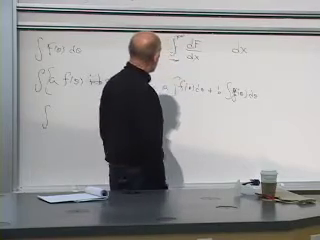
\includegraphics[width=0.88\textwidth]{lecture_06_figure_05.png}
\lectureframe{01:26:31.594}
\caption{베레진 적분의 일반적인 원형은 전체 도함수의 적분이 경계값으로 환원되며 함수가 충분히 빠르게 감쇠하면 적분값도 사라진다는 것이다. 아래쪽 칠판 줄은 일부 가려져 있어 본문에 식을 옮겨 적었다.}
\end{figure}

그라스만 적분이 선형이고 전미분의 적분이 0이 되는 유용한 성질을 공유하도록 하자. 홀수 좌표 하나에 대해서는 다음을 요구한다.
\begin{align}
\int d\theta\,[af(\theta)+bg(\theta)]
&=
a\int d\theta\,f(\theta)
+b\int d\theta\,g(\theta),\\
\int d\theta\,\partial_\theta f(\theta)&=0.
\end{align}
두 번째 조건은 측도의 병진 불변성에 해당하는 대수적 조건이다. 홀수 수직선에는 끝점이 없으며, 작은 구간에 대한 합도 없다.

\begin{classroomqa}\audiencequestion{부정 그라스만 적분이 없다면, 적분이 미분의 역연산이라는 생각을 포기하는 건가요? \lecturetimestamp{01:21:19}}\lecturerresponse{그렇다. 베레진 적분은 원시함수 연산이 아니라 정적분을 주는 선형 함수다. 그라스만 변수 하나의 경우에는 실제로 미분과 같은 대수적 연산으로 나타난다.}\end{classroomqa}

\begin{classroomqa}\audiencequestion{시공간 전체에 대한 \(d^4x\) 적분도 정적분인가요? \lecturetimestamp{01:21:34}}\lecturerresponse{그렇다. 작용을 시공간에 대해 적분할 때는 경계 조건을 전제한다. 차이는 보통 시공간 적분은 합의 극한으로 이해할 수 있는 반면, 그라스만 적분은 유한한 기저 \(1,\theta\)에 작용하는 방식으로 대수적으로 정의된다는 점이다.}\end{classroomqa}

\subsection{변수 하나}

홀수 변수 하나의 모든 함수는 계수를 정해진 오른쪽 순서로 놓아 다음과 같이 쓸 수 있다.
\begin{equation}
f(\theta)=a+\theta b.
\end{equation}
\(\partial_\theta\theta=1\)이므로, 전미분 규칙에 따라 다음을 얻는다.
\begin{equation}
\int d\theta\,1=0.
\end{equation}
나머지 정규화는 다음과 같이 정한다.
\begin{equation}
\int d\theta\,\theta=1.
\end{equation}
따라서
\begin{equation}
\int d\theta\,f(\theta)=b.
\end{equation}
적분은 가능한 최고 차수 항의 계수를 추출한다. 여기서 사용하는 좌미분 규약에서는
\begin{equation}
\partial_\theta f=b
=\int d\theta\,f.
\end{equation}

\begin{classroomqa}\audiencequestion{조건 \(\partial_\theta F=\theta\)을 만족하는 함수 \(F(\theta)\)가 있나요? \lecturetimestamp{01:30:05}}\lecturerresponse{없다. 그런 함수에는 \(\theta^2\)에 비례하는 항이 있어야 하지만 \(\theta^2=0\). 이는 그라스만 변수에서 부정 적분에 해당하는 것이 없는 이유를 보여주는 또 다른 방식이다.}\end{classroomqa}

\subsection{변수 두 개와 적분 측도의 순서}

복소 변수 쌍 \(\theta,\bar\theta\)에 대해 일반적인 짝수 함수를 정해진 순서로 쓰면 다음과 같다.
\begin{equation}
f(\theta,\bar\theta)
=a+\bar\theta\psi+\bar\psi\theta+b\,\bar\theta\theta.
\end{equation}
\begin{equation}
\theta^2=\bar\theta^2=0,
\qquad
\bar\theta\theta=-\theta\bar\theta.
\end{equation}이므로 더 높은 차수 항은 없다.

이제 다음 규약을 정한다.
\begin{equation}
\int d\theta\,d\bar\theta\,
\bar\theta\theta=1.
\end{equation}
반복 적분에서는 인접한 \(d\bar\theta\) 연산이 먼저 작용한다. 그러면 표는 다음과 같다.
\begin{align}
\int d\theta\,d\bar\theta\,1&=0,\\
\int d\theta\,d\bar\theta\,\theta&=0,\\
\int d\theta\,d\bar\theta\,\bar\theta&=0,\\
\int d\theta\,d\bar\theta\,\bar\theta\theta&=1.
\end{align}
따라서
\begin{equation}
\int d\theta\,d\bar\theta\,
f(\theta,\bar\theta)=b.
\end{equation}

\begin{classroomqa}
\audiencequestion{\(\theta\)에 선형인 항에서는 이중 적분을 사라지게 하는 것이 정말 \(\theta\) 적분인가요?\lecturetimestamp{01:34:59}}
\lecturerresponse{아니다. 강의 중 설명에서 두 적분의 역할이 뒤바뀌어 있었다. \(\theta\)를 \(\theta\)에 대해 적분하면 1이 된다. 그러면 결과에는 더 이상 \(\bar\theta\)가 없고, 남은 \(\bar\theta\)에 대한 적분은 1을 적분하므로 사라진다. 어느 경우든 두 변수가 모두 들어 있어야 이중 적분이 살아남는다.}
\end{classroomqa}

\begin{classroomqa}\audiencequestion{\(\theta\)와 \(\bar\theta\)의 순서를 바꾸면 적분의 부호가 바뀌나요? \lecturetimestamp{01:36:33}}\lecturerresponse{그렇다. 홀수 변수와 홀수 측도는 서로 반가환한다. 위에서 정한 규약에서는
\[
\int d\bar\theta\,d\theta\,\bar\theta\theta=-1.
\]
따라서 순서를 하나 정해 일관되게 유지해야 한다. 물리는 규약에 무관하지만 중간 계산의 부호는 그렇지 않다.}\end{classroomqa}

서로 독립인 그라스만 변수가 \(n\)개일 때는 규칙을 바로 일반화할 수 있다.
\begin{equation}
\int d\theta_n\cdots d\theta_1\,
f(\theta_1,\ldots,\theta_n)
\end{equation}
이 적분은 변수와 측도에 대해 선택한 순서로 정해지는 부호까지 고려하면, 정렬된 최고차 단항식 \(\theta_1\cdots\theta_n\)의 계수를 추출한다. 이 간단한 성분 추출 규칙이 초공간 작용의 핵심이다. 초대칭 변분은 홀수 전미분이 되고, 초공간 적분은 이를 제거한다. 적절한 경계 조건 아래 보통 작용이 시공간 전미분을 제거하는 것과 같다.

\section{이처럼 단순한 계산법이 강력한 이유}

규칙은 거의 자명해 보인다:
\begin{equation}
\int d\theta\,1=0,
\qquad
\int d\theta\,\theta=1.
\end{equation}
그럼에도 이 규칙으로 보손과 페르미온의 질량 및 결합 상수 사이의 관계가 자동으로 유지되는 상호작용 장론을 구성할 수 있다. 초공간 계산법의 목적은 상대론에서 텐서 계산법의 목적과 같다. 허용된 모든 조작을 거쳐도 원하는 대칭성이 유지되도록 표기를 구성하는 것이다.

그 대가로 부호를 꼼꼼히 따져야 한다. 홀수인 두 대상을 맞바꿀 때마다 마이너스 부호가 생기며, 개념적으로는 옳은 계산도 순서를 한 번 잘못 정하면 틀릴 수 있다. 이 어려움은 장식적인 것이 아니라 페르미온 통계가 대수에 드리우는 흔적이다.

\begin{classroomqa}\audiencequestion{그라스만 수는 초대칭과 함께 발명되었나요, 아니면 더 일찍 등장했나요? \lecturetimestamp{01:41:19}}\lecturerresponse{그라스만 수는 훨씬 오래되었다. 헤르만 그라스만은 19세기에 그 기초가 되는 외대수를 발전시켰다. 미분형식에는 이미 반가환 기저 원소가 쓰인다. 20세기 양자장론과 초대칭은 같은 수학에서 새로운 물리적 역할을 발견했다.}\end{classroomqa}

이제 구체적인 구성을 살펴볼 준비가 되었다. 초장은 보손과 페르미온으로 이루어진 완전한 다중항을 담고, 초공간 미분은 대수 구조를 보존하며, 베레진 적분은 성분 작용을 추출한다. 다음으로 이 도구를 가장 단순한 1차원 모형에 적용한 뒤 장론으로 확장한다.

\chapter{초공간과 초대칭 동역학의 구성}

\lectureoverview{초대칭이 작용할 수 있는 가장 작은 계, 즉 에너지가 같은 보손 조화진동자 하나와 페르미온 조화진동자 하나에서 출발해 초대칭을 다시 구성한다. 두 계의 방정식이 각각 2계와 1계라는 차이에서 초전하와 그 대수가 나온다. 이어서 그 대수를 보통 좌표 (t)와 그라스만 좌표 \(\theta,\bar\theta\)를 갖는 공간 위의 기하학으로 재해석한다. 초장은 보손, 페르미온, 보조장을 하나의 대상으로 묶고, 베레진 적분은 불변인 보통 라그랑지안을 추출하며, 공변미분은 대칭과 양립하는 제약을 가능하게 한다. 카이랄 제약은 그 첫 번째 중요한 예다. 이 강의에서는 이 형식론에서 부호와 순서를 다루기 어렵다는 점을 숨기지 않고 보여준 뒤, 대칭 자체가 파인만 규칙의 목록보다 왜 더 근본적인지 설명하며 마무리한다.}

\section{한 모드 계로 돌아가기}

정지한 페르미온과 보손에서 다시 시작하자. 모든 공간 좌표와 운동량 표기는 생략한다. 각 모드에는 양자가 있거나 없으며, 생성 연산자와 소멸 연산자만으로 이를 기술할 수 있다. 보손 모드는 \(a^\dagger,a\), 페르미온 모드는 \(c^\dagger,c\)로 쓰자. 이들은 다음 관계를 만족한다.
\begin{align}
[a,a^\dagger]&=1,
&
\{c,c^\dagger\}&=1,
&
c^2=(c^\dagger)^2&=0.
\end{align}
두 양자의 에너지가 같아 \(m\)이면, 무시해도 되는 진공 상수를 제외하고 해밀토니안은 다음과 같다.
\begin{equation}
H=m\left(a^\dagger a+c^\dagger c\right).
\label{eq:l7-one-mode-hamiltonian}
\end{equation}
수 연산자 \(a^\dagger a\)는 음이 아닌 정수 값을 취할 수 있지만, \(c^\dagger c\)은 0 또는 1만 취할 수 있다. 이것이 이 장난감 모형의 운동학 전부다.

이 단순화는 전략적인 선택이다. 에너지를 바꾸지 않으면서 보손을 없애고 페르미온을 넣거나, 그 반대의 일을 하는 연산을 이해하고자 한다. 하지만 그 연산을 구성하기 전에, 같은 계를 연산자 언어에서 라그랑지안 언어로 옮겨 보자.

\section{보손 조화진동자}

보손에 대해 실수 좌표 \(\phi(t)\)를 도입하자. 공간적으로 변하지 않는 자유 스칼라장은 보통 조화진동자가 된다. 칠판에 처음 적힌 식은 다음과 같았다.
\[
\frac{1}{2}\dot\phi^{,2}+\frac{1}{2}m^2\phi^2.
\]
이 식은 운동에너지와 퍼텐셜에너지의 합이지 라그랑지안이 아니다. 강의에서는 곧바로 부호를 바로잡는다.
\begin{equation}
L_B=\frac{1}{2}\dot\phi^{,2}-\frac{1}{2}m^2\phi^2.
\label{eq:l7-boson-lagrangian}
\end{equation}

\begin{figure}[H]
\centering
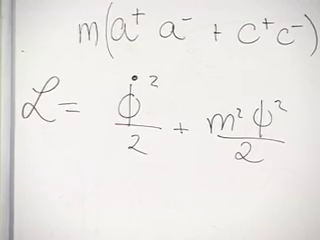
\includegraphics[width=0.62\textwidth]{lecture_07_figure_02.png}
\lectureframe{00:03:25.431}
\caption{보손 라그랑지안 위에 놓인 한 모드 해밀토니안. 화면은 말로 수정하기 전의 처음 부호가 플러스였던 점을 보존한다. \(T-V\)}
\end{figure}

\begin{classroomqa}
\audiencequestion{화면에 표시된 조화진동자 라그랑지안에서 부호가 잘못된 이유는 무엇인가? \lecturetimestamp{00:04:00}}
\lecturerresponse{에너지는 \(T+V\)이지만 라그랑지안은 \(T-V\)이다. 따라서 퍼텐셜 항에는 마이너스 부호가 붙어야 한다. 이 수정으로 방정식은 지수적으로 변하는 거동을 나타내는 식에서 의도한 조화진동을 나타내는 식으로 바뀐다.}
\end{classroomqa}

실제로 오일러--라그랑주 방정식은 다음을 준다.
\begin{align}
\frac{d}{dt}\frac{\partial L_B}{\partial\dot\phi}
&=\frac{\partial L_B}{\partial\phi},\\
\ddot\phi&=-m^2\phi,
\end{align}
즉,
\begin{equation}
\ddot\phi+m^2\phi=0.
\label{eq:l7-boson-eom}
\end{equation}
진동수는 \(m\)이지 \(m^2\)가 아니다. 이 조화진동자를 양자화하면 식 ~\eqref{eq:l7-one-mode-hamiltonian}의 \(a^\dagger\)와 \(a\)가 기술하는 것과 같은 상태 사다리를 얻는다.

\section{페르미온 작용이 1계인 이유}

페르미온 라그랑지안은 시간 미분이 하나뿐이어서 더 단순해 보인다. 그 이유는 의도적으로 단순한 시도에서 이미 드러난다. 서로 교환하는 보통 변수에 대해서는
\begin{equation}
L_{\mathrm{trial}}=\phi\dot\phi
=\frac{1}{2}\frac{d}{dt}\phi^2.
\end{equation}
이것은 전미분이다. 이에 따른 오일러--라그랑주 방정식은 \(\dot\phi=\dot\phi\)만을 말하므로, 미분 가능한 모든 경로가 허용된다. 작용에서 전미분을 빼도 끝점 자료는 달라지지만 운동 방정식의 벌크 부분은 달라지지 않는다.

이제 변수를 \(\psi\)로 바꾸고 그라스만 홀수 변수라고 하자. \(\psi\)와 \(\dot\psi\)는 모두 반교환한다. 왼쪽 변분을 택하면 홀수 인자들의 순서를 바꿀 때 마이너스 부호가 생기므로, 같은 형식의 시도에서 다음을 얻는다.
\begin{equation}
\frac{d}{dt}\frac{\partial L_{\mathrm{trial}}}{\partial\dot\psi}
=\dot\psi,
\qquad
\frac{\partial L_{\mathrm{trial}}}{\partial\psi}
=-\dot\psi.
\end{equation}
따라서 방정식은 다음과 같다.
\begin{equation}
\dot\psi=-\dot\psi
\quad\Longrightarrow\quad
\dot\psi=0.
\label{eq:l7-constant-fermion}
\end{equation}
서로 교환하는 좌표에서는 항등식에 불과했던 식이 반교환하는 좌표에서는 동역학적 내용을 갖게 되었다. 이 식은 조화진동자를 기술하기에는 내용이 지나치게 많아서 상수해만 허용하지만, 바로 그것이 필요한 실마리다.

\begin{classroomqa}
\audiencequestion{해가 단지 \(\psi\)가 상수라는 뜻인가? \lecturetimestamp{00:13:57}}
\lecturerresponse{그렇다. 식~\eqref{eq:l7-constant-fermion}은 실제 1계 미분방정식이며, 그 해는 임의의 그라스만 값 상수다. 질량항을 더하면 이 정적인 해가 진동하는 해로 바뀐다.}
\end{classroomqa}

당연해 보이는 시도인 \(m\psi^2\)는 \(\psi^2=0\)이므로 실패한다. 실수 홀수 변수 \(\psi_1,\psi_2\) 두 개가 필요하며, 이는 복소 변수 하나와 그 켤레로 바꾸어 쓸 수 있다. 강의에서는 칠판에 실수 변수 두 개를 쓰는 형식을 전개하며 부호와 2의 인자를 거듭 확인한다. 표준적인 정규화를 택한 복소 형식은 다음과 같다.
\begin{equation}
L_F=\frac{i}{2}
\left(\bar\psi\dot\psi-\dot{\bar\psi}\psi\right)
-m\bar\psi\psi.
\label{eq:l7-fermion-lagrangian}
\end{equation}
전미분을 무시하면 이는 \(i\bar\psi\dot\psi-m\bar\psi\psi\)이다. \(\bar\psi\)에 대해 변분하면 다음을 얻는다.
\begin{equation}
i\dot\psi=m\psi,
\qquad
\psi(t)=\psi(0)e^{-imt}.
\label{eq:l7-fermion-eom}
\end{equation}
켤레 방정식은 위상 부호가 반대다. 따라서 페르미온 모드는 보손 모드와 마찬가지로 에너지 \(m\)로 진동하지만, 그 방정식은 2계가 아니라 1계다.

\editorialnote{방정식~\eqref{eq:l7-fermion-lagrangian}은 실수 변수 두 개를 사용하는 탐색적 계산에서 표준적인 배열과 정규화 한 가지를 정한다. 강의에서는 여기에 \(i\)를 곱하고, 계수를 두 배 조정하며, 실수 성분 하나의 부호는 확정하지 않는다. 이러한 차이에도 핵심 결론은 달라지지 않는다. 페르미온의 운동항은 일차 미분형이고, 질량은 선형으로 나타나며, 복소 페르미온은 영이 아닌 쌍선형항을 만든다.}

이는 익숙한 상대론적 대비를 0차원으로 축소한 모습이다. 클라인--고든 방정식은 시간에 대해 2계인 반면, 디랙 방정식은 1계다. 공간을 생략하면 보손은 조화진동자 하나가 되고 페르미온은 복소 그라스만 조화진동자 하나가 된다.

\begin{classroomqa}
\audiencequestion{\(\psi\)와 \(\dot\psi\) 및 그 켤레를 쓰는 순서가 중요한가? \lecturetimestamp{00:18:58}}
\lecturerresponse{홀수 인자가 반교환하므로 중간 식은 순서에 따라 달라진다. 하지만 왼쪽 변분 또는 오른쪽 변분, 켤레화, 적분에 이르기까지 하나의 규약을 일관되게 사용하면 물리 이론은 임의의 표기 선호에 좌우되지 않는다. 홀수 인자 한 쌍의 순서를 뒤집으면 부호가 바뀌며, 다른 모든 곳에서도 일관되게 부호를 바꾸어야 한다.}
\end{classroomqa}

식~\eqref{eq:l7-boson-lagrangian}과 \eqref{eq:l7-fermion-lagrangian}를 결합하면 식~\eqref{eq:l7-one-mode-hamiltonian}이 나타내는 동일한 에너지 짝을 라그랑지안으로 기술할 수 있다. 이제 두 모드 사이의 대칭을 확인할 준비가 되었다.

\section{초전하와 그 대수}

페르미온을 없애고 보손을 넣는 연산자는 다음과 같다.
\begin{equation}
Q^\dagger=\sqrt{2m}\,a^\dagger c,
\end{equation}
켤레 연산자는 보손을 없애고 페르미온을 넣는다.
\begin{equation}
Q=\sqrt{2m}\,a c^\dagger.
\end{equation}
대수의 표준형을 얻도록 정규화를 택했다. \(cc^\dagger=1-c^\dagger c\), \(aa^\dagger=a^\dagger a+1\)와 보손 연산자와 페르미온 연산자가 서로 교환한다는 사실을 사용하면,
\begin{align}
\{Q,Q^\dagger\}
&=2m\left(ac^\dagger a^\dagger c+a^\dagger c a c^\dagger\right)\notag\\
&=2m\left[(a^\dagger a+1)c^\dagger c
+a^\dagger a(1-c^\dagger c)\right]\notag\\
&=2m\left(a^\dagger a+c^\dagger c\right)=2H.
\label{eq:l7-superalgebra}
\end{align}
보손 연산자는 페르미온 연산자를 지나 이동할 수 있다. 페르미온 점유를 제한하는 같은 멱등성으로부터 다음을 얻는다.
\begin{equation}
Q^2=(Q^\dagger)^2=0.
\end{equation}
마지막으로,
\begin{equation}
[H,Q]=[H,Q^\dagger]=0.
\label{eq:l7-conserved-supercharges}
\end{equation}
각 초전하는 보손 수와 페르미온 수를 서로 반대 방향으로 바꾼다. 따라서 진동수가 같으면 두 변화에 따른 에너지가 상쇄된다.

\begin{classroomqa}
\audiencequestion{\([H,Q]\)는 무엇인가? 답은 \(Q\)에 비례하는가? \lecturetimestamp{00:25:10}}
\lecturerresponse{아니다. 답은 0이다. 생성 또는 소멸 연산자 하나만 있다면 \(H\)와의 교환에서 그 에너지가 드러나겠지만, \(Q\)에 들어 있는 보손 항과 페르미온 항은 서로 상쇄된다. 이 상쇄가 바로 두 에너지가 같다는 조건이다.}
\end{classroomqa}

\begin{classroomqa}
\audiencequestion{그 교환자를 칠판에 이미 쓰지 않았나? \lecturetimestamp{00:25:45}}
\lecturerresponse{그렇다. 다시 찾아내는 과정은 관계를 그저 베끼지 않고 해석하게 해 준다는 점에서 유용하다. 해밀토니안과 교환한다는 것은 그 변환이 대칭이며 그 생성자가 보존된다는 뜻이다.}
\end{classroomqa}

\emph{전하}라는 말은 이 보존 법칙을 가리킨다. 그렇다고 \(Q\)을 상태에 붙는, 동시에 측정할 수 있는 보통 수처럼 취급해서는 안 된다. 이것은 그라스만 홀수이고 멱영이며 보손 상태를 페르미온 상태로 사상한다. 유용한 진술은 이것이 축퇴 초다중항 안에서 작용하는 보존 생성자라는 것이다.
\editorialnote{이 설명은 상태를 에너지나 전하로 분류하는 교실의 비유를 더 정확하게 다듬는다. 개별적인 비에르미트 홀수 초전하는 수치 양자값을 갖는 보통 관측량이 아니다. 올바른 분류는 이들의 보존된 작용과 완전한 초대수의 표현으로 주어진다.}

\section{미분 연산자로서의 생성자}

대수는 간결하지만, 그것만으로는 상호작용 이론을 어떻게 구성할지 알 수 없다. 다음 단계는 기하학이다. 익숙한 대칭 생성자도 이미 미분 연산자로 작용한다. 강의의 규약에서는
\begin{equation}
H=i\frac{\partial}{\partial t},
\qquad
P=-i\frac{\partial}{\partial x}.
\end{equation}

\begin{figure}[H]
\centering
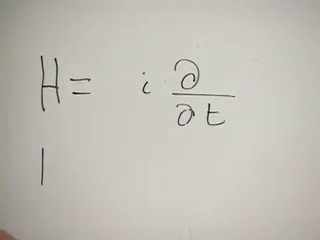
\includegraphics[width=0.50\textwidth]{lecture_07_figure_03.png}
\lectureframe{00:28:12.720}
\caption{시간 병진의 생성자로 나타낸 해밀토니안.}
\end{figure}

각운동량도 마찬가지로 좌표와 미분의 곱이다. 초전하가 홀수 생성자라면 홀수 좌표에 대한 미분으로 나타낼 수 있는지 묻는 것이 자연스럽다. 따라서 시간축을 다음 초공간으로 확장한다.
\begin{equation}
(t,\theta,\bar\theta),
\qquad
\theta^2=\bar\theta^2=0,
\qquad
\theta\bar\theta=-\bar\theta\theta.
\end{equation}
이 공간 위의 장은 보통 시간과 켤레인 그라스만 좌표 한 쌍에 의존한다.

강의에서는 부호가 얼마나 까다로운지 의도적으로 드러낸다. 복소켤레를 취할 때 생기는 부호, 홀수 매개변수를 옮길 때 생기는 부호, 왼쪽 미분과 오른쪽 미분 중 어느 쪽을 택하느냐에 따른 부호는 서로 다른 연산에서 나온다. 서로 양립하지 않는 칠판상의 전개 단계를 그대로 유지하는 대신, 여기서는 하나의 규약을 정한다. 모든 홀수 미분은 왼쪽 미분으로 둔다.
\begin{equation}
q=\partial_\theta+i\bar\theta\partial_t,
\qquad
\bar q=\partial_{\bar\theta}+i\theta\partial_t.
\label{eq:l7-differential-supercharges}
\end{equation}
그러면
\begin{equation}
q^2=\bar q^{,2}=0,
\qquad
\{q,\bar q\}=2i\partial_t=2H.
\label{eq:l7-differential-algebra}
\end{equation}
두 배 인자는 두 교차항 \(\{\partial_\theta,\theta\}=1\)와 \(\{\partial_{\bar\theta},\bar\theta\}=1\)에서 나온다. 생성자에 \(\partial_\theta\)와 \(\partial_{\bar\theta}\)만 들어 있다면 반교환자는 영이 되어 해밀토니안을 재현할 수 없다.

\begin{classroomqa}
\audiencequestion{\(q\)와 \(\bar q\)의 시간 미분 항 두 개는 같은 부호를 가져야 하나? \lecturetimestamp{00:31:01}}
\lecturerresponse{혼합 반교환자가 \(2H\)이 되도록 부호를 일관되게 정해야 한다. 전체적으로 플러스인 규약이나 그에 맞게 켤레를 취한 규약을 모두 사용할 수 있다. 기호 \(i\)에 대한 직관이 아니라 계산이 상대 부호를 정한다.}
\end{classroomqa}

강의실에서는 부호를 거듭 확인하고, 출근길에 부호가 바뀌는 것 같다는 농담도 나온다. 적절한 농담이다. 물리적 규약이 전혀 바뀌지 않았더라도 그라스만 매개변수를 좌표 사이로 옮기면 부호가 바뀔 수 있다. 뒤에 나오는 모든 내용은 식~\eqref{eq:l7-differential-supercharges}을 고정된 기준으로 삼는다.

\subsection{좌표 이동으로서의 초대칭}

무한소 홀수 매개변수 \(\xi,\bar\xi\)를 두자. 초장에
\begin{equation}
\delta_\xi=\xi q+\bar\xi\bar q
\end{equation}
를 작용시키는 것은 위 규약에서 다음 무한소 좌표 변환과 동등하다.
\begin{align}
\theta&\longrightarrow\theta+\xi,\\
\bar\theta&\longrightarrow\bar\theta+\bar\xi,\\
t&\longrightarrow t+i\left(\xi\bar\theta+\bar\xi\theta\right).
\label{eq:l7-coordinate-shift}
\end{align}
따라서 스칼라 초장의 변화는 다음과 같다.
\begin{equation}
\delta_\xi\Phi
=\left(\xi\partial_\theta+\bar\xi\partial_{\bar\theta}
+i\xi\bar\theta\partial_t+i\bar\xi\theta\partial_t\right)\Phi
=\left(\xi q+\bar\xi\bar q\right)\Phi.
\end{equation}
이것이 초대칭의 기하학적 내용이다. 이는 홀수 방향으로의 병진이며, 보통 시간 방향의 병진과 결부되어 있다. 홀수 이동 두 번의 합성은 식~\eqref{eq:l7-differential-algebra}에 따라 시간 병진으로 닫힌다.

\begin{classroomqa}
\audiencequestion{논란이 된 마이너스 부호는 시간을 거슬러 움직인다는 뜻일 수 있나? \lecturetimestamp{00:58:13}}
\lecturerresponse{다른 부호 규약을 택하면 표시된 무한소 시간 이동의 방향이 반대가 될 수 있지만, 별개의 물리적 과거 방향 시간 과정이 도입되는 것은 아니다. 중요한 것은 좌표 변환과 미분 생성자가 같은 대수를 따른다는 점이다.}
\end{classroomqa}

\begin{classroomqa}
\audiencequestion{이렇게 확장한 시간에는 물리적 실현이 있는가, 아니면 형식적인 계산 도구일 뿐인가? \lecturetimestamp{00:58:23}}
\lecturerresponse{유용한 의미에서 이는 대수를 기하학으로 묶어 표현하는 계산 도구다. 하지만 상호작용을 도입하면 그 표현이 물리적으로 유용해진다. 초공간은 텐서 미적분이 로런츠 스칼라를 구성하는 데 도움이 되듯, 모든 단계에서 보손--페르미온 대칭을 보존하는 라그랑지안을 구성하는 체계적인 계산법을 제공한다.}
\end{classroomqa}

\section{초장과 보조 성분}

홀수 좌표가 둘뿐이므로 짝수 초장의 전개는 유한한 항에서 끝난다.
\begin{equation}
\Phi(t,\theta,\bar\theta)
=\phi(t)+\bar\theta\psi(t)+\bar\psi(t)\theta
+D(t)\bar\theta\theta.
\label{eq:l7-superfield}
\end{equation}
짝수 차수 단항식 \(\phi\)와 \(D\)의 계수는 보손이고, 홀수 차수 단항식 \(\psi\)와 \(\bar\psi\)의 계수는 페르미온이다. \(\theta^2\), \(\bar\theta^2\) 또는 그 이상의 항은 남지 않는다. \(t\)에 대한 보통 테일러 급수는 유한한 항에서 끝나지 않고 여기서는 쓸모가 없으므로 시간 의존성은 전개하지 않는다.

\begin{classroomqa}
\audiencequestion{맨 위 항의 성분 \(D(t)\)는 무엇인가? \lecturetimestamp{00:41:46}}
\lecturerresponse{이 단계에서는 유한 전개에서 마지막에 놓인 보손 계수일 뿐이다. 성분 작용에서는 보통 운동항이 없고 대수적인 운동 방정식으로 제거되므로 보조장이라고 부른다. 강의에서는 ``D는 dummy의 D''라는 장난스러운 설명도 나오는데, 이는 이 장의 비동역학적 역할을 잘 나타내지만 역사적 정의는 아니다.}
\end{classroomqa}

초장은 하나의 대상이고 \(\phi,\psi,\bar\psi,D\)는 그 성분들이다. 초대칭 변환은 이 성분들을 서로 섞는다. 따라서 보손과 페르미온은 벡터의 \(x\) 성분과 \(y\) 성분이 회전으로 서로 연결되는 것과 구조적으로 매우 비슷한 방식으로 관련되어 있다. 다만 그라스만 방향을 보통 축처럼 그릴 수는 없다.

\section{초작용과 맨 위 성분}

운동 방정식을 얻으려면 작용이 필요하다. 보통 장론에서는 스칼라 라그랑지안을 만든 뒤 시공간에 대해 적분한다. 여기서 이에 대응하는 식은 다음과 같다.
\begin{equation}
S=\int dt\,d\theta\,d\bar\theta\;\Lambda
\bigl(\Phi,\text{ superspace derivatives of }\Phi\bigr),
\label{eq:l7-superaction}
\end{equation}
여기서 \(\Lambda\)은 짝수 초장이다. 베레진 적분은 대수적이다. 다음을 택하자.
\begin{equation}
\int d\theta\,d\bar\theta\;\bar\theta\theta=1.
\end{equation}
따라서
\begin{equation}
\Lambda=A+\bar\theta B+\bar B\theta+C\bar\theta\theta,
\end{equation}
이면,
\begin{equation}
\int d\theta\,d\bar\theta\;\Lambda=C.
\label{eq:l7-top-component}
\end{equation}
홀수 적분은 맨 위 성분을 추출해 남기며, 이를 시간에 대해 적분하면 보통 라그랑지안을 얻는다.

결과가 불변인 이유는 무엇일까? 초대칭 변환은 적분 변수를 평행이동시킨다. 최고 성분의 변분은 시간에 대한 통상적인 전미분인 반면, 홀수 전미분은 베레진 적분에서 사라진다. 적절한 경계 조건 아래에서 작용은 변하지 않는다. 이는 시공간에 대해 적분하기 전에 로런츠 스칼라를 구성하는 것에 대응하는 초공간의 방법이다.

\section{초장 곱하기}

기존 초장으로 새 초장을 만드는 가장 간단한 방법은 그 초장을 자기 자신과 곱하는 것이다. 식~\eqref{eq:l7-superfield}에서 시작하면 \(\theta^2\) 또는 \(\bar\theta^2\)가 포함된 모든 항은 사라진다. 순서를 \(\bar\theta\theta\)로 유지하고 켤레 성분장을 왼쪽에 쓰면 다음을 얻는다.
\begin{align}
\Phi^2
={}&\phi^2
+2\phi\bar\theta\psi
+2\phi\bar\psi\theta\notag\\
&+\left(2\phi D-2\bar\psi\psi\right)\bar\theta\theta.
\label{eq:l7-superfield-square}
\end{align}

\begin{figure}[H]
\centering
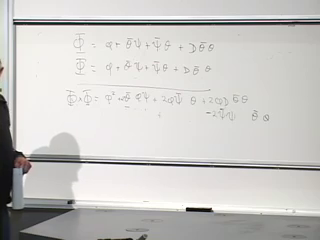
\includegraphics[width=0.82\textwidth]{lecture_07_figure_05.png}
\lectureframe{01:07:57.844}
\caption{성분별로 전개한 초장 곱과 그 \(\bar\theta\theta\) 항들을 모아 나타낸 그림.}
\end{figure}

두 항 \(\phi D\)와 \(D\phi\)는 둘 다 짝수장이므로 더해진다. 두 페르미온 교차항도 각각 순서를 바꾸면 더해지지만, 두 항 모두 마이너스 부호를 갖는다.
\begin{equation}
(\bar\theta\psi)(\bar\psi\theta)
+(\bar\psi\theta)(\bar\theta\psi)
=-2\bar\psi\psi\,\bar\theta\theta.
\end{equation}
제곱을 홀수 좌표에 대해 적분하면 다음을 얻는다.
\begin{equation}
\int d\theta\,d\bar\theta\;\Phi^2
=2\phi D-2\bar\psi\psi.
\end{equation}
이 항은 구성상 초대칭이지만, 아직 운동항을 갖는 라그랑지안은 아니다. 시간 미분이 없다.

이어서 칠판에는 \(\Phi^3\), \(\Phi^4\), \(\Phi^n\)를 연습 문제로 제시한다. 간단한 규칙이 있다. 임의의 보통 함수 \(W\)에 대해
\begin{equation}
\left.W(\Phi)\right|_{\bar\theta\theta}
=W'(\phi)D-W''(\phi)\bar\psi\psi.
\label{eq:l7-function-top-component}
\end{equation}
\(W(\phi)=\phi^2\)의 경우에는 식~\eqref{eq:l7-superfield-square}가 재현되고, \(W(\phi)=\phi^n\)의 경우에는 다음을 얻는다.
\begin{equation}
\left.\Phi^n\right|_{\bar\theta\theta}
=n\phi^{n-1}D-n(n-1)\phi^{n-2}\bar\psi\psi.
\end{equation}
\editorialnote{\(n\)제곱의 경우는 연습 문제로 제시하면서 예상되는 항의 종류를 설명한다. 식~\eqref{eq:l7-function-top-component}은 고정된 순서 규약에서 완성된 규칙을 제공한다.}

이때 강사는 강의실 사람들이 지쳤는지 묻는다. 청중은 아니라고 답하고, 강사는 자신은 지쳤다고 말한다. 이 대화는 단순한 웃음거리에 그치지 않는다. 초장 거듭제곱은 전개가 유한하게 끝나므로 다루기 쉽지만, 부호 계산이 실제로 까다로워지는 곳은 미분과 제약이다.

\section{초대칭을 따르는 미분은 무엇인가?}

다음 칠판 논의를 따라가기 전에 한 가지를 바로잡아야 한다. 보통 시간 미분은 문제가 없다.
\begin{equation}
[\partial_t,q]=[\partial_t,\bar q]=0.
\end{equation}
따라서 \(\Phi\)가 초장이면 \(\partial_t\Phi\)도 초장으로 변환된다. 까다로운 것은 맨몸 홀수 미분 \(\partial_\theta\Phi\)와 \(\partial_{\bar\theta}\Phi\)이다. 이 미분들은 두 초전하 모두와 반교환하지 않기 때문이다. 제약을 두고 초대칭 성분 구성을 명시적으로 하는 데에는 수정된 홀수 미분이 필요하다.
\editorialnote{시간 미분을 하면 또 다른 초장이 되지 않는다는 강의 중 발언은 여기서 사용한 규약에서는 옳지 않다. \(\partial_t\)는 두 초전하 모두와 교환하므로 공변적이다. 수정된 홀수 미분을 뒤이어 구성하는 과정은 여전히 필요하며, 그것이 강의에서 다루는 실제 수학적 요점이다.}

\subsection{``마법장 비유''}

강의에서는 보통 회전을 예로 들어 기준을 설명한다. \(f(x,y)\)가
\begin{equation}
\partial_y f=0.
\label{eq:l7-magic-constraint}
\end{equation}
을 만족한다고 하자. 이런 함수를 ``매직장''이라고 부르자. 이 함수는 \(x\)에는 의존하지만 \(y\)에는 의존하지 않는다. 회전해도 매직장들의 집합이 보존되는가? 다음에 대해서는
\begin{equation}
L_z=-i\left(x\partial_y-y\partial_x\right),
\end{equation}
다음이 성립한다.
\begin{equation}
[\partial_y,L_z]=i\partial_x\neq0.
\end{equation}
따라서 \(L_z f\)는 일반적으로 \(y\)에 의존하게 된다. 처음에 \(f\)가 식~\eqref{eq:l7-magic-constraint}을 만족하더라도 마찬가지다. 이 제약은 회전 불변이 아니다.

일반적인 원리는 간단하다. 장이 \(C\Phi=0\)을 만족하고 대칭이 \(G\)에 의해 생성된다면, \(C\)와 \(G\)의 등급 교환자가 영일 때 변환된 장도 제약 조건을 만족한다. 두 연산자가 모두 홀수이면 등급 교환자는 반교환자이다.

\begin{classroomqa}
\audiencequestion{장에 대한 제약이 대칭과 양립하는 조건은 무엇인가? \lecturetimestamp{01:17:56}}
\lecturerresponse{제약 연산자가 대칭 생성자들과 등급 교환할 때다. 그러면 \(C(G\Phi)\)에서 \(G\)를 옮겨 \(G(C\Phi)=0\)로 바꿀 수 있다. 회전 예에서는 \(\partial_y\)가 회전 생성자와 교환하지 않으므로 제약이 보존되지 않는다.}
\end{classroomqa}

\subsection{공변 홀수 미분}

초전하를 식~\eqref{eq:l7-differential-supercharges}로 정하고 다음을 정의하자.
\begin{equation}
\mathcal D=\partial_\theta-i\bar\theta\partial_t,
\qquad
\bar{\mathcal D}=\partial_{\bar\theta}-i\theta\partial_t.
\label{eq:l7-covariant-derivatives}
\end{equation}
바뀌는 것은 시간 미분 항의 부호뿐이다. 직접 계산하면 다음을 얻는다.
\begin{align}
\{\mathcal D,q\}
&=\{\mathcal D,\bar q\}
=\{\bar{\mathcal D},q\}
=\{\bar{\mathcal D},\bar q\}=0,\\
\{\mathcal D,\bar{\mathcal D}\}&=-2i\partial_t.
\label{eq:l7-covariant-algebra}
\end{align}
영이 아닐 수 있는 두 교차항은 서로 상쇄된다. 이는 홀수 연산자에 대응하는 공변미분이다. 변환 법칙을 보존하면서 미분한다.

강의에서는 보조 성분과 이 미분 연산자를 모두 \(D\)로 표기한다. 성분은 \(D(t)\)로 남겨 두고 연산자는 필기체 \(\mathcal D\)로 표기하겠다.

\section{카이랄 제약}

이제 초대칭 아래에서 보존되는 비자명한 제약을 부과할 수 있다.
\begin{equation}
\bar{\mathcal D}\Phi=0.
\label{eq:l7-chiral-constraint}
\end{equation}
이런 장을 카이랄이라고 한다. 초대칭 변환 전의 장이 카이랄이면,
\begin{equation}
\bar{\mathcal D}(q\Phi)
=-q(\bar{\mathcal D}\Phi)=0,
\qquad
\bar{\mathcal D}(\bar q\Phi)
=-\bar q(\bar{\mathcal D}\Phi)=0.
\end{equation}
따라서 변환된 초장 전체가 제약된 집합 안에 남는다. 매직장 조건과 달리 카이랄성은 대칭과 양립한다.

제약을 풀기 위해 이동된 시간 좌표를 정의하자.
\begin{equation}
\tau=t+i\bar\theta\theta.
\label{eq:l7-chiral-time}
\end{equation}
왼쪽 미분을 사용하므로
\begin{equation}
\partial_{\bar\theta}\tau=i\theta,
\end{equation}
따라서
\begin{equation}
\bar{\mathcal D}F(\tau,\theta)
=\left(\partial_{\bar\theta}-i\theta\partial_t\right)F(\tau,\theta)
=i\theta\partial_\tau F-i\theta\partial_\tau F=0.
\end{equation}
일반적인 국소 카이랄 초장은 \(\bar\theta\)에 \(\tau\)를 통해서만 의존한다.
\begin{equation}
\Phi_{\mathrm{ch}}(\tau,\theta)
=\phi(\tau)+\bar\psi(\tau)\theta.
\label{eq:l7-chiral-field-tau}
\end{equation}

\begin{classroomqa}
\audiencequestion{\(\tau\)와 \(\theta\)에 의존하는 형태만 카이랄 제약을 만족하는가? \lecturetimestamp{01:32:35}}
\lecturerresponse{국소적으로는 그렇다. 미분 방정식 \(\bar{\mathcal D}\Phi=0\)은 독립적인 \(\bar\theta\) 의존성을 이동된 좌표 \(\tau=t+i\bar\theta\theta\)에 흡수할 수 있다는 뜻이다. 나머지 유한 전개는 \(\tau\)의 함수와 \(\theta\)에 비례하는 항 하나로 이루어진다.}
\end{classroomqa}

원래 시간 좌표로 다시 전개하면,
\begin{align}
\phi(\tau)
&=\phi(t)+i\bar\theta\theta\dot\phi(t),\\
\bar\psi(\tau)\theta
&=\bar\psi(t)\theta,
\end{align}
두 번째 줄의 보정항은 \(\theta^2\)를 포함하기 때문이다. 따라서
\begin{equation}
\Phi_{\mathrm{ch}}(t,\theta,\bar\theta)
=\phi(t)+\bar\psi(t)\theta
+i\bar\theta\theta\dot\phi(t).
\label{eq:l7-chiral-field-components}
\end{equation}

\begin{classroomqa}
\audiencequestion{\(\phi(t+i\bar\theta\theta)\)의 테일러 전개에 2차 항도 들어가야 하지 않나? \lecturetimestamp{01:33:51}}
\lecturerresponse{아니다. 첫 번째 보정항은 \(i\bar\theta\theta\dot\phi\)이고, 그보다 높은 차수의 모든 보정항에는 \((\bar\theta\theta)^2=0\)가 들어간다. 청중은 이를 곧바로 알아차린다. 멱영성 때문에 이미 첫 두 항만 남고 급수가 끝난다.}
\end{classroomqa}

이것이 카이랄성의 간결함이다. 제약되지 않은 초장인 식~\eqref{eq:l7-superfield}에는 보손 성분 자리 두 개와 페르미온 성분 자리 두 개가 있다. 이 최소 1차원 예에서는 카이랄 조건이 독립적인 보조장 자리를 없애고 맨 위 성분을 \(\dot\phi\)에 결부한다.

\section{제대로 멈춘 계산}

자연스럽게 다음으로 할 일은 카이랄 장과 그 켤레를 결합해 초공간에서 적분하는 것이다. 켤레 전개를 시작하자 청중 한 사람이 켤레화할 때 순서 \(\theta\bar\theta\)를 뒤집어야 하는지 묻는다. 그 시점에는 부호를 더는 믿기 어렵다. 허세를 부리는 대신 계산을 멈춘다.

\begin{classroomqa}
\audiencequestion{켤레장 곱셈은 미루더라도 핵심 결과를 말해 줄 수 있는가? \lecturetimestamp{01:37:30}}
\lecturerresponse{그렇다. 부호와 켤레화를 일관되게 처리하면 카이랄 장과 그 켤레로 만든 초공간 식에서 원하는 보통 보손 및 페르미온 운동항을 얻는다. 이 강의의 중요한 결과는 믿기 어려운 계산 끝부분을 그대로 옮기는 것이 아니라 구성 원리다.}
\end{classroomqa}

계산을 멈춘 지점을 분명히 남겨 두어야 한다. 이 형식론에서는 홀수 인자 하나의 위치만 잘못되어도 부호가 바뀌며, 켤레화와 미분, 곱셈, 적분을 거치면서 같은 규약을 유지해야 한다. 그 연결이 끊겼다면 계속하기 전에 바로잡아야 한다. 표준 규약에서 익숙한 운동 작용은 켤레 곱으로 구성되지만, 성분으로 자세히 전개하는 일은 끝나지 않은 칠판 식을 복원하는 과정이 아니라 다음 번에 정확히 계산할 몫이다.

\section{대칭이 핵심인 이유}

초대칭 라그랑지안은 보손과 페르미온을 나란히 놓는 데 그치지 않는다. 이들의 질량과 상호작용을 제약해 초대수의 표현을 이루게 한다. 초대칭이 정확한 진공에서는 초다중항을 이루는 입자들의 질량이 같다. 이들의 고리 보정 기여는 서로 연관되어 있으며, 보손과 페르미온의 자외선 효과는 대칭이 정하는 조합에서 상쇄된다.

이 때문에 구성 형식론이 중요하다. 파인만 꼭짓점을 나열해 상쇄를 다이어그램마다 확인할 수도 있지만, 그러면 상쇄가 우연처럼 보인다. 초대칭은 로런츠 대칭이 모든 관성계에서 산란 진폭이 일관되게 변환되는 이유를 설명하는 것과 같은 방식으로 그 상쇄를 설명한다.

\editorialnote{정확한 초대칭이 개별 자체에너지 보정이 모두 사라진다는 뜻은 아니다. 초대칭은 재규격화를 서로 연관시키고 특정 자외선 민감성을 없애지만, 비재규격화 정리의 성립 여부는 대상량과 차원, 초대칭의 양에 달려 있다. 강의의 폭넓은 상쇄 주장은 이처럼 조건을 명시한 형태로 유지한다.}

\begin{classroomqa}
\audiencequestion{``카이랄''은 어떻게 철자하는가? \lecturetimestamp{01:39:48}}
\lecturerresponse{C-H-I-R-A-L. 이 말은 제약 \(\bar{\mathcal D}\Phi=0\)을 가리킨다. 3차원 공간에서 물체가 갖는 보통의 기하학적 손잡이성은 아니다. 다만 이 용어는 상대론적 스피너의 왼손 및 오른손 구조에서 유래했다.}
\end{classroomqa}

\begin{classroomqa}
\audiencequestion{라그랑지안을 거치지 않고 초대칭 파인만 규칙으로 바로 넘어갈 수 있는가? \lecturetimestamp{01:40:00}}
\lecturerresponse{규칙 자체를 제시할 수는 있지만, 결합상수 사이의 관계와 그에 따른 상쇄가 설명되지 않은 우연처럼 보일 것이다. 더 깊은 내용은 일반화된 시공간 대칭이다. 라그랑지안이나 그에 동등한 불변 형식은 그 이유를 드러내고 규칙을 체계적으로 도출한다.}
\end{classroomqa}

섭동의 모든 차수에서 로런츠 변환을 한 번도 언급하지 않았는데도 로런츠 불변 진폭이 나온다고 가정해 보자. 계산을 충분히 거듭하고 나면 우리는 설명을 요구할 것이다. 그 답은 모든 차수를 한꺼번에 조직하는 시공간 대칭일 것이다. 초공간의 역할도 이와 비슷하다. \(\theta,\bar\theta\)에서의 이동은 보손 성분과 페르미온 성분을 서로 섞으며, 그 대수는 시공간 병진으로 닫힌다.

\begin{classroomqa}
\audiencequestion{그라스만 좌표처럼 보통의 공간 좌표도 유한 거듭제곱 급수로 전개해야 하나요? \lecturetimestamp{01:44:55}}
\lecturerresponse{아니다. 보통 좌표에 대한 거듭제곱 급수는 끝나지 않으며, 대개 자연스러운 분해 방식도 아니다. 장을 파동과 운동량으로 분해하는 푸리에 변환이 더 유용하다. \(\theta\)로 전개하는 방식이 특별한 까닭은 멱영성 때문에 급수가 유한하게 끝나기 때문이다.}
\end{classroomqa}

\begin{classroomqa}
\audiencequestion{LHC에서 새로운 입자가 발견되면, 그것이 단지 미지의 입자가 아니라 초대칭 짝입자임을 어떻게 알아낼 수 있나요? \lecturetimestamp{01:45:42}}
\lecturerresponse{초대칭은 단지 하나의 추가 상태가 아니라 서로 연관된 양자수와 상호작용을 예측한다. 스핀은 1/2만큼 차이가 나고, 게이지 전하들은 서로 연관되며, 많은 세제곱 및 네제곱 결합은 일반적인 이론에서보다 적은 수의 독립 매개변수로 정해진다. 산란 단면적, 붕괴 분기비, 그리고 나머지 입자 스펙트럼이 이러한 관계들을 만족해야 한다.}
\end{classroomqa}

낯선 공명 하나만으로 초대칭이 입증되지는 않는다. 결합 상수와 입자 스펙트럼 사이의 관계망이 입증의 근거가 될 것이다. 이것이 초공간 구성에 대응하는 실험적 측면이다. 겉보기에는 서로 독립적인 성분 상호작용들이 하나의 불변량에서 나온다.

\begin{classroomqa}
\audiencequestion{관측된 입자와 가설적인 초대칭 짝입자의 질량은 같지 않습니다. 이것은 이론을 어떻게 바꾸나요? \lecturetimestamp{01:47:01}}
\lecturerresponse{이론을 크게 바꾼다. 초대칭은 깨져야 하며, 보통 자발적 대칭 깨짐이 관측 부문에 전달되는 방식으로 이루어진다. 대칭 깨짐은 다중항의 질량을 갈라놓으면서도 상호작용을 제어할 만큼, 그리고 깨짐 에너지 척도가 충분히 낮다면 자외선 보정을 제어할 만큼의 구조를 보존한다. 이 메커니즘을 구체적으로 밝히는 일은 그 자체로 상당한 이론적 과제이며, 중력을 포함하면 특히 그렇다.}
\end{classroomqa}

\section{단순한 원리, 어려운 계산}

마무리 평가는 유난히 솔직하다. 출발점의 발상은 단순해 보인다. 보손과 페르미온이 대칭으로 연결되어 있다는 것이다. 하지만 이를 구체화하는 과정은 곧 지표, 켤레, 그라스만 변수의 순서, 부호를 다루는 학문으로 발전한다. 대칭을 구성한 뒤에도 현실적인 입자물리학을 위해서는 대칭을 깨야 하며, 중력과 결합하면 초중력으로 이어져 구조가 한층 더 복잡해진다.

이 어려움이 발상이 공허하다는 증거는 아니다. 자연은 단순한 원리를 계산하기 쉽게 만들어야 할 의무가 없다. 전문가들은 부호 규칙이 몸에 밸 때까지 세부 계산을 거듭하며 이 주제를 익힌다. 답답함은 간결한 대수
\begin{equation}
\{Q,Q^\dagger\}=2H
\end{equation}
와 상호작용하는 이론에서 이를 구현하는 데 필요한 방대한 계산 체계 사이의 간극에서 생긴다.

\begin{classroomqa}
\audiencequestion{추상화의 층을 하나 더 쌓으면 결국 형식이 단순해지나요, 아니면 복잡성이 계속 늘어나나요? \lecturetimestamp{01:49:33}}
\lecturerresponse{세부 계산을 없애 주는 일반적인 단순화 방법은 없다. 기본 규칙은 짧을 수 있지만, 이를 믿을 수 있게 적용하려면 규약을 반복해서 정확히 다뤄야 한다. 그래서 이 주제를 제대로 다루려면 보통 광범위한 입자물리학 강의의 일부가 아니라 하나의 기술 과목 전체가 필요하다.}
\end{classroomqa}

\begin{classroomqa}
\audiencequestion{이 변환은 페르미온과 보손이 실제로 무엇인지, 또는 두 입자의 통상적인 거동이 왜 다른지를 알려 주나요? \lecturetimestamp{01:51:42}}
\lecturerresponse{두 입자가 하나의 초장(superfield)을 이루는 성분이며 초전하에 의해 서로 대응하는 상임을 알려 준다. \(Q\)을 작용시키면 보손 성분이 페르미온 성분으로 변환되고, 다음 변환에서는 미분과 보조 성분이 생긴다. 이는 회전이 벡터의 성분들을 서로 섞는 것과 비슷하지만, 똑같이 문자 그대로인 그림으로 옮길 수는 없다. 여기에 적합한 언어는 그라스만 기하학 자체다.}
\end{classroomqa}

이 답은 우리를 핵심 발상으로 되돌린다. 초대칭 변환은 초공간에서의 미소한 변환이다. 보통 회전이 성분들을 서로 섞듯이 \(\phi,\psi,\bar\psi,D\)를 서로 섞으며, 그 대수는 시간 병진으로 닫힌다. 이 그림은 추상적이지만 자의적이지 않다. 초장의 모든 항, 공변미분의 모든 부호, 성분 상호작용 사이의 모든 관계는 대수를 구현하기 위해 존재한다.

\section{우리가 구성한 것}

짝을 이루는 진동자 해밀토니안에서 시작해 서로 다른 두 가지 라그랑지안 기술을 되찾았다. 보손은 2계 진동자 방정식을 따르고, 페르미온에는 1계 그라스만 작용과 홀수 성분의 복소수 쌍이 필요하다. 초전하들은 두 모드를 서로 바꾸며, 각각 제곱하면 0이 되고, 서로 반교환하면 해밀토니안을 내놓으며, 해밀토니안과는 교환한다.

이 전하들을 미분 연산자로 표현하면서 초공간에 이르렀다. 유한한 초장 전개로 보손, 페르미온, 보조 성분을 한데 모았고, 베레진 적분으로 초라그랑지안의 최고차 성분을 골라냈으며, 곱셈으로 불변 상호작용 후보를 만들었다. 이어서 대칭과 양립하는 홀수 미분을 요구하자 \(\mathcal D,\bar{\mathcal D}\), 카이랄 제약 조건, 그리고 이동된 좌표 \(\tau=t+i\bar\theta\theta\)가 도입되었다.

끝내 마무리하지 않은 켤레 곱 계산도 감춰야 할 결함이 아니라 이 수업의 일부다. 초대칭은 단순한 물리적 요구에서 출발하지만, 그 계산법은 순서를 정하는 모든 선택에 민감하다. 그 선택들을 제대로 다루고 나면 큰 보상이 따른다. 질량과 결합 상수가 대칭에 따라 조직되고, 양자 보정은 우연이 아닌 관계를 만족하며, 보손과 페르미온은 하나의 기하학적 대상의 성분이 된다.

\chapter{4차원 초대칭과 웨스--지노 모형}

\lectureoverview{앞 강의의 1차원 초대칭 대수에는 해밀토니안만 등장했다. 이제 로런츠 불변성에 따라 에너지는 공간 운동량과 다시 하나로 묶이고, 초전하들은 2성분 스피너가 되어야 한다. 먼저 질량이 없는 바일 페르미온과 그 해밀토니안 \(H=\boldsymbol{\sigma}\cdot\mathbf p\)으로 돌아가 이 대수에 이른다. 이어 초전하를 4차원 초공간의 미분 연산자로 나타내고, 구속 조건 \(\bar D_{\dot\alpha}\Phi=0\)으로 카이랄 초장을 분리한 다음, 초공간 적분을 사용해 구체적인 장 이론을 구성한다. 차례로 \(\Phi^\dagger\Phi\), \(\Phi^2\), \(\Phi^3\)을 택하면 전파항, 같은 보손--페르미온 질량, 유카와 상호작용, 그리고 이에 연결된 스칼라 상호작용이 생긴다. 보조장 \(F\)을 도입하면 이러한 관계가 명확해지고, 마지막 루프 도표는 초대칭이 자외선 민감도를 완화하는 이유를 보여 준다.}

\section{해밀토니안만으로는 충분하지 않은 이유}

장난감 모형에서는 공간을 생략하고 기본 관계를 다음과 같이 썼다.
\begin{equation}
\{Q,Q^\dagger\}=2H.
\label{eq:l8-time-only-algebra}
\end{equation}
시간만이 좌표인 경우에는 이 형태로 충분하다. 그러나 상대론적 이론에서 \(H=P_0\)는 4-운동량 \(P_\mu\)의 한 성분이다. 로런츠 부스트를 하면 \(P_i\)와 섞인다. 따라서 우변에서 \(P_0\)만을 특별히 취하는 대수는 공변적으로 변환될 수 없다.

그러므로 이 문제를 해결하려면 두 가지를 동시에 해야 한다. \(H\)를 네 성분 모두인 \(P_\mu\)로 바꾸고, 우변의 로런츠 벡터와 대응할 수 있는 지표를 좌변에 마련해야 한다. 질량이 없는 디랙 방정식이 필요한 실마리를 준다. 상대론적 페르미온은 2성분 스피너로 기술할 수 있고, 행렬 \(\sigma^\mu\)는 벡터 지표를 두 개의 스피너 지표로 변환한다.

\section{질량 없는 페르미온, 헬리시티, 카이랄성}

먼저 질량이 있는 입자와 질량이 없는 입자의 물리적 차이를 살펴보자. 스핀-\(\tfrac12\) 입자가 스핀 방향으로 움직인다고 하자. 이 입자의 속력은 빛의 속력보다 작으므로 관찰자가 입자를 앞지를 수 있다. 새 기준계에서는 운동량 방향이 뒤집히지만 스핀 방향은 그대로이므로 헬리시티가 뒤집힌다. 따라서 로런츠 불변인 질량 있는 이론에는 두 헬리시티가 모두 포함되어야 한다.

질량이 없는 입자는 어떤 관찰자도 앞지를 수 없다. 적절한 로런츠 변환으로는 스핀에 대한 운동량의 방향을 뒤집을 수 없으므로, 하나의 기약 질량 없는 표현은 한 가지 헬리시티만 가질 수 있다. 공간 회전으로 진행 방향을 반대로 돌릴 수는 있지만, 오른손을 왼손으로 바꾸지는 못한다.

\begin{classroomqa}
\audiencequestion{앞지르기 논증은 정말 카이랄성이 아니라 헬리시티에 관한 것인가요? \lecturetimestamp{00:05:42}}
\lecturerresponse{그렇다. 헬리시티는 운동량 방향으로 투영한 스핀인 반면, 카이랄성은 카이랄 행렬의 고윳값이며 통상 \(\gamma^5\)로 표기한다. 질량 없는 모드에서는 두 표지가 서로 연결되어 있어 이 예에서는 두 용어가 서로 바꿔 쓸 수 있는 것처럼 들린다. 질량이 있는 입자에서는 서로 구별된다.}
\end{classroomqa}

상태 수를 말할 때는 한 가지 단서를 붙여야 한다.\editorialnote{질량 없는 바일 장 하나에는 입자 헬리시티 하나와 그 반대 헬리시티를 가진 반입자가 있다. 따라서 “상태 수가 절반”이라는 말은 4성분 디랙 장에서 2성분 바일 장 하나로 줄어드는 것을 뜻한다. 반입자 상태가 사라졌다는 뜻은 아니다.}

이 도입부 논증에서 사용하는 바일 장을 다음과 같이 쓰자.
\begin{equation}
\chi=
\begin{pmatrix}
\chi_1\\
\chi_2
\end{pmatrix},
\end{equation}
강의에서는 이 장을 \(\psi_\alpha\)로 표기한다. 아래에서 카이랄 초장에 통상 포함되는 켤레 바일 표현과 혼동하지 않도록 여기서는 \(\chi\)라고 부르겠다.
\begin{equation}
H\chi=\boldsymbol{\sigma}\cdot\mathbf p\,\chi.
\label{eq:l8-weyl-hamiltonian}
\end{equation}
운동량 \(\mathbf p\)에 대해 행렬 \(\boldsymbol{\sigma}\cdot\mathbf p\)의 고윳값은 \(\pm|\mathbf p|\)이다. 양의 주파수 가지는 입자 모드를 제공한다. 음의 주파수 가지는 아래로 무한히 뻗는 스펙트럼으로 남겨 두는 대신 반입자 구성으로 재해석한다.

\begin{figure}[H]\centering
\includegraphics[width=0.70\textwidth]{lecture_08_figure_02.png}\lectureframe{00:07:44.271}\caption{카이랄 2성분 스피너와 해밀토니안 \(H=\boldsymbol{\sigma}\cdot\mathbf p\). 마지막 운동량 기호 일부가 가려져 있지만, 강의에서 말한 방정식으로 확인할 수 있다.}\end{figure}

손잡이성 표지는 관례에도 좌우된다.\editorialnote{칠판에서는 \(\boldsymbol{\sigma}\cdot\mathbf p\)의 양의 고윳값에 손잡이성을 직접 대응시킨다. 어느 카이랄성에 그 부호를 붙일지는 \(\sigma^\mu\), \(\bar\sigma^\mu\), 바일 장을 어떻게 정의하느냐에 달려 있다. 고윳값에 관한 진술은 유지하되, 관례와 무관한 좌·우 표지는 붙이지 않는다.}

\(H\)를 \(i\partial_t\)로, \(\mathbf p\)를 \(-i\nabla\)로 바꾸면 다음을 얻는다.
\begin{equation}
i\partial_t\chi=-i\boldsymbol{\sigma}\cdot\nabla\chi.
\end{equation}
이제 다음을 도입하자.
\begin{equation}
\begin{aligned}
\sigma^\mu&=(\mathbf 1,\boldsymbol{\sigma}),\\
\bar\sigma^\mu&=(\mathbf 1,-\boldsymbol{\sigma}),\\
\eta_{\mu\nu}&=\operatorname{diag}(1,-1,-1,-1).
\end{aligned}
\label{eq:l8-sigma-convention}
\end{equation}
그러면 방금 얻은 방정식은 다음과 같다.
\begin{equation}
i\sigma^\mu\partial_\mu\chi=0.
\label{eq:l8-weyl-equation}
\end{equation}
켤레 바일 표현에는 \(\bar\sigma^\mu\)를 사용한다. 아래에서 \(\psi_\alpha\)라고 부르는 것이 바로 이 켤레 표현이며, 이 표현의 자유 방정식은 \(i\bar\sigma^\mu\partial_\mu\psi=0\)이다. 공변성을 증명하려면 로런츠 군의 스피너 표현이 필요하지만, 여기서 중요한 점은 구조다. 네 행렬 \(\sigma^\mu\)가 하나의 시공간 지표를 두 개의 스피너 지표와 연결한다.

\section{4차원 초대수}

이제 홀수 좌표는 바일 스피너처럼 변환해야 한다.
\begin{equation}
\theta^\alpha=(\theta^1,\theta^2),
\qquad
\bar\theta^{\dot\alpha}=(\bar\theta^{\dot1},\bar\theta^{\dot2}).
\end{equation}
바는 복소켤레를 나타내며, 점은 켤레 로런츠 표현을 구별한다. 그래스만 성분은 복소수 두 개, 즉 실수 네 개다. 일반적인 짝수 초장
\begin{equation}
\mathcal S=\mathcal S(x^\mu,\theta^\alpha,\bar\theta^{\dot\alpha})
\end{equation}
은 따라서 유한한 그래스만 전개를 갖는다. 최고차 단항식은
\begin{equation}
\theta^2\bar\theta^2
\equiv
(\theta^1\theta^2)(\bar\theta^{\dot1}\bar\theta^{\dot2}),
\end{equation}
독립적인 홀수 좌표 네 개를 모두 곱한 것이다. 이 단항식의 계수를 통상 \(D\) 성분이라고 부른다.

초전하에도 스피너 지표가 붙는다. 4차원 \(N=1\) 초대칭에서 초전하 대수는 다음과 같다.
\begin{align}
\{Q_\alpha,\bar Q_{\dot\beta}\}
&=2\sigma^\mu_{\alpha\dot\beta}P_\mu,
\label{eq:l8-superalgebra-main}\\
\{Q_\alpha,Q_\beta\}&=0,
&
\{\bar Q_{\dot\alpha},\bar Q_{\dot\beta}\}&=0,
\label{eq:l8-superalgebra-nilpotent}\\
[P_\mu,Q_\alpha]&=0,
&
[P_\mu,\bar Q_{\dot\alpha}]&=0,
&
[P_\mu,P_\nu]&=0.
\label{eq:l8-superalgebra-commutators}
\end{align}
계수 2는 관례에 따른다. 행렬
\(\sigma^\mu_{\alpha\dot\beta}\)은 \(P_\mu\)의 벡터 지표를 수축해 좌변에 나타나는 두 스피너 지표만 남긴다.

\begin{classroomqa}
\audiencequestion{시그마 행렬의 \(\alpha\)와 \(\beta\)는 행렬 지표인가요? \lecturetimestamp{00:22:01}}
\lecturerresponse{그렇다. 더 정확히 말하면 하나는 점 없는 바일 지표이고 다른 하나는 점이 있는 켤레 지표다. \(\mu\)는 시공간 벡터 지표다. 시그마 행렬은 이 두 기술 방식 사이를 이어 준다.}
\end{classroomqa}

정돈한 표기법은 이 연결을 명시적으로 드러낸다.\editorialnote{강의에서는 점 지표를 의도적으로 생략하고 칠판에서 \(\alpha\beta\)와 \(\beta\alpha\) 중 어느 순서가 맞는지 논의한다. ~\eqref{eq:l8-superalgebra-main}과 \eqref{eq:l8-superalgebra-commutators}은 논증의 내용은 바꾸지 않으면서 표준적인 점 지표·점 없는 지표 표기를 복원한다.}

마지막 줄은 초전하가 보존되고 병진과 양립함을 말한다. 미분 연산자로 나타내면 운동량 성분들은 서로 교환한다. 아래에서 사용하는 미분 표기법에서는
\begin{equation}
P_\mu=i\partial_\mu,
\end{equation}
따라서 식 ~\eqref{eq:l8-superalgebra-main}은 다음과 같이 써도 된다.
\begin{equation}
\{Q_\alpha,\bar Q_{\dot\beta}\}
=2i\sigma^\mu_{\alpha\dot\beta}\partial_\mu.
\end{equation}

\section{초공간 미분으로 나타낸 초전하}

운동량은 보통 좌표를 병진시키지만, 초전하는 시공간도 함께 이동시키면서 홀수 좌표를 병진시킨다. 왼쪽 그래스만 미분을 택하고 다음과 같이 정의하자.
\begin{align}
Q_\alpha
&=\partial_\alpha
-i\sigma^\mu_{\alpha\dot\alpha}
\bar\theta^{\dot\alpha}\partial_\mu,
\label{eq:l8-Q}\\
\bar Q_{\dot\alpha}
&=-\bar\partial_{\dot\alpha}
+i\theta^\alpha\sigma^\mu_{\alpha\dot\alpha}\partial_\mu.
\label{eq:l8-Qbar}
\end{align}
\(\epsilon^\alpha Q_\alpha+
\bar\epsilon_{\dot\alpha}\bar Q^{\dot\alpha}\)를 작용시키면 초장에 대한 무한소 초대칭 변분을 얻는다. 그 성분은 독립적인 그래스만 단항식들의 계수일 뿐이며, 미분 연산자는 이 계수들을 서로 섞는다.

\begin{classroomqa}\audiencequestion{약식 표기 \(\bar\theta\sigma\partial\)에서 어떤 \(x\) 미분을 뜻하나요? \lecturetimestamp{00:25:40}}\lecturerresponse{네 성분 모두를 뜻한다. \(\bar\theta^{\dot\alpha}\sigma^\mu_{\alpha\dot\alpha}\partial_\mu\)에 반복된 \(\mu\) 지표를 합산하므로, \(\sigma^\mu\)의 각 성분은 그에 대응하는 미분 \(\partial/\partial x^\mu\)와 짝을 이룬다.}\end{classroomqa}

\begin{classroomqa}\audiencequestion{켤레 전하에는 또 다른 \(\bar\theta\)가 아니라 \(\theta\)가 들어가야 하나요? \lecturetimestamp{00:26:16}}\lecturerresponse{그렇다. \(Q\)는 \(\theta\)에 대해 미분하고 \(\bar\theta\)를 포함한다. \(\bar Q\)는 \(\bar\theta\)에 대해 미분하고 \(\theta\)를 포함한다. 두 연산자는 서로 켤레다.}\end{classroomqa}

\begin{classroomqa}\audiencequestion{\(\sigma^\mu\)는 대칭인가요? \lecturetimestamp{00:27:04}}\lecturerresponse{파울리 행렬은 에르미트다. \((\mathbf1,\boldsymbol{\sigma})\)의 네 행렬 가운데 세 개는 대칭이고, \(\sigma^2\)는 보통 전치에 대해 반대칭이다. 여기서 관련된 켤레 성질은 에르미트성에 점 지표와 점 없는 지표의 배치를 함께 고려한 것이다.}\end{classroomqa}

\begin{classroomqa}\audiencequestion{켤레 방정식의 시그마 행렬은 지표를 반대 순서로 갖나요? \lecturetimestamp{00:27:13}}\lecturerresponse{켤레화하면 점 지표 표현과 점 없는 지표 표현이 서로 바뀐다. 따라서 두 표지를 서로 바꿔 쓸 수 있는 행렬 슬롯처럼 취급하기보다 \(\sigma^\mu_{\alpha\dot\alpha}\)와 그 켤레 \(\bar\sigma^{\mu\,\dot\alpha\alpha}\)로 표기하는 것이 안전하다.}\end{classroomqa}

식 ~\eqref{eq:l8-Q}와 \eqref{eq:l8-Qbar}의 표기는 칠판의 약식 표기와 겉보기 부호가 다르다. 이 부호는 \(P_\mu\)를 \(+i\partial_\mu\)로 정의하는지 \(-i\partial_\mu\)로 정의하는지, 미분이 왼쪽에서 작용하는지 오른쪽에서 작용하는지, 켤레 홀수 변수를 어떤 순서로 배열하는지에 따라 달라진다. 중요한 것은 하나의 관례가 대수 전체를 일관되게 만족한다는 점이다.

\section{초대칭 아래에서도 유지되는 구속 조건}

일반적인 초장에는 성분이 많다. 대칭성을 깨뜨리지 않으면서 더 작은 종류의 장을 찾고자 한다. 강의에서는 먼저 보통 벡터를 예로 든다. 벡터 \(\mathbf V\)에 대해 구속 조건
\begin{equation}
V_x=0
\end{equation}
은 회전 불변이 아니다. 회전하면 \(V_y\)가 새로운 \(x\) 성분에 기여한다. 반면
\begin{equation}
\mathbf V^2=1
\end{equation}
은 불변이며 독립적인 자유도 하나를 없앤다. 유용한 구속 조건은 대칭 변환 후에도 구속된 장을 구속된 장으로 보내야 한다.

선형 홀수 연산자 \(\bar D_{\dot\alpha}\)가 다음을 정의한다고 하자.
\begin{equation}
\bar D_{\dot\alpha}\Phi=0.
\label{eq:l8-chiral-constraint}
\end{equation}
초대칭 변분 \(\delta\Phi=Q\Phi\)을 가한 뒤에도 같은 조건이 유지되려면 \(\bar D\)가 초전하와 반가환하면 된다.
\begin{equation}
\bar D(Q\Phi)=-Q(\bar D\Phi)=0.
\end{equation}
이는 설명 없이 제시하는 정의가 아니라, 이 구성을 이끄는 추상적인 일관성 조건이다.

\begin{classroomqa}\audiencequestion{마지막 식에서 \(Q\)와 \(\bar D\)를 왜 서로 바꿀 수 있나요? \lecturetimestamp{00:36:56}}\lecturerresponse{이들은 반가환하도록 택한 홀수 연산자다. 따라서 순서를 바꾸면 마이너스 부호가 붙는다. \(\bar D\)가 \(\Phi\)에 작용하면 원래 구속 조건에 따라 결과는 0이 된다.}\end{classroomqa}

필요한 공변 미분은 초전하에 비해 시공간 미분의 부호를 뒤집어 얻는다.
\begin{align}
D_\alpha
&=\partial_\alpha
+i\sigma^\mu_{\alpha\dot\alpha}
\bar\theta^{\dot\alpha}\partial_\mu,
\label{eq:l8-D}\\
\bar D_{\dot\alpha}
&=-\bar\partial_{\dot\alpha}
-i\theta^\alpha\sigma^\mu_{\alpha\dot\alpha}\partial_\mu.
\label{eq:l8-Dbar}
\end{align}
이들은 다음 관계를 만족한다.
\begin{align}
\{D_\alpha,\bar D_{\dot\beta}\}
&=-2i\sigma^\mu_{\alpha\dot\beta}\partial_\mu,\\
\{D_\alpha,Q_\beta\}
&=\{D_\alpha,\bar Q_{\dot\beta}\}=0,\\
\{\bar D_{\dot\alpha},Q_\beta\}
&=\{\bar D_{\dot\alpha},\bar Q_{\dot\beta}\}=0.
\end{align}

\begin{classroomqa}\audiencequestion{\(\bar Q\)에서 \(\bar D\)로 바뀔 때 시공간 미분항의 부호만 바뀌나요? \lecturetimestamp{00:37:58}}\lecturerresponse{그렇다. 이 부호를 뒤집으면 \(D\)를 어느 초전하와 반교환할 때든 교차항이 상쇄된다.}\end{classroomqa}

식 ~\eqref{eq:l8-chiral-constraint}만 부과한다. \(D_\alpha\Phi=0\)와 \(\bar D_{\dot\alpha}\Phi=0\)를 모두 부과하면 두 식의 반교환자로 인해 \(\partial_\mu\Phi=0\)가 되어, 시공간에 무관한 나머지만 남을 수 있다.
\editorialnote{칠판에서는 두 구속 조건을 모두 부과하면 \(\Phi=0\)가 된다고 말한다. 대수적으로 엄밀히 따라오는 것은 장이 시공간에 무관하다는 결론이다. 추가적인 경계 조건이나 성분 조건을 부과하면 장을 더 제한할 수 있다.}

\section{카이랄 구속 조건 풀기}

이동된 좌표를 다음과 같이 정의하자.
\begin{equation}
y^\mu=x^\mu+i\theta\sigma^\mu\bar\theta.
\label{eq:l8-chiral-coordinate}
\end{equation}
위에서 정한 왼쪽 미분 관례에 따르면 함수
\begin{equation}
\Phi=\Phi(y,\theta)
\label{eq:l8-chiral-solution}
\end{equation}
은 \(\bar D_{\dot\alpha}\Phi=0\)을 만족한다. 연쇄 법칙을 적용하면 상쇄가 명확히 드러난다. \(y^\mu\)를 미분하면 \(i\theta\sigma^\mu\partial_\mu\Phi\) 항이 생기며, 이 항은 \(\bar D_{\dot\alpha}\)에 나타나는 같은 항과 부호가 반대다.

따라서 카이랄 초장에는 독립적인 \(\bar\theta\) 의존성이 없다. \(\bar\theta\)는 포함될 수 있지만, 오직 조합 \(y^\mu\)을 통해서만 나타난다. 유한 전개는 다음과 같다.
\begin{equation}
\Phi(y,\theta)
=\phi(y)+\sqrt2\,\theta\psi(y)+\theta^2F(y).
\label{eq:l8-chiral-expansion-y}
\end{equation}
세 가지 성분 유형은 복소 스칼라 \(\phi\), 바일 페르미온 \(\psi_\alpha\), 복소 스칼라 \(F\)다. 마지막 성분은 전파하는 두 번째 보손이 아니라 보조장이다.

\begin{classroomqa}\audiencequestion{\(x\)을 그것과 직교하는 새 좌표 \(y\)로 바꾼 건가요? \lecturetimestamp{00:49:08}}\lecturerresponse{아니다. \(y^\mu\)는 식 ~\eqref{eq:l8-chiral-coordinate}에 나오는 특정 조합을 간단히 나타낸 표기다. 추가적인 시공간 방향이 아니다. \(y\)를 사용하면 카이랄성을 간단히 표현할 수 있고, 보통의 장 이론을 구성할 때는 다시 \(x\)로 돌아간다.}\end{classroomqa}

~\eqref{eq:l8-chiral-expansion-y}에서 \(x\)를 고정한 채 전개하면 다음과 같다.
\begin{align}
\Phi(x,\theta,\bar\theta)
={}&\phi
+\sqrt2\,\theta\psi
+\theta^2F
+i\theta\sigma^\mu\bar\theta\,\partial_\mu\phi
\notag\\
&-\frac{i}{\sqrt2}\theta^2
\partial_\mu\psi\,\sigma^\mu\bar\theta
+\frac14\theta^2\bar\theta^2\Box\phi.
\label{eq:l8-chiral-expansion-x}
\end{align}
우변의 모든 성분장은 \(x\)에서 계산한다. 켤레 안티카이랄 장은 \(\bar y^\mu=x^\mu-i\theta\sigma^\mu\bar\theta\)와 \(\bar\theta\)에 의존한다. 카이랄 초장은 실수일 수 없다. 그 켤레가 반대 카이랄성 구속 조건을 만족하기 때문이다.

\section{초공간 적분}

초공간 전체에 대한 작용은 다음 형태다.
\begin{equation}
S_D=\int d^4x\,d^2\theta\,d^2\bar\theta\;K,
\label{eq:l8-D-term-action}
\end{equation}
여기서 \(K\)는 실수 초장이다. 베레진 적분은 그 \(\theta^2\bar\theta^2\) 성분을 선택한다. 홀수 변수에 대한 적분을 마치면 보통의 시공간 라그랑지안만 남는다.

불변인 구성을 하나 더 만들 수 있다. \(W(\Phi)\)가 카이랄이면,
\begin{equation}
S_F=\int d^4x\,d^2\theta\;W(\Phi)
+\int d^4x\,d^2\bar\theta\;\overline{W}(\Phi^\dagger)
\label{eq:l8-F-term-action}
\end{equation}
은 초대칭 불변이다. 첫 번째 적분은 \(\theta^2\) 성분을, 두 번째 적분은 그 켤레를 선택한다.

\begin{classroomqa}\audiencequestion{\(\bar\theta\) 의존성이 없는 식을 \(d^2\theta\)에 대해서만 적분해도 되는 이유는 무엇인가요? \lecturetimestamp{01:16:30}}\lecturerresponse{카이랄성은 초대칭 변환 아래에서 보존되며, 카이랄 초장의 최고차 \(\theta\) 성분은 시공간 전미분만큼만 변한다. 따라서 시공간 적분은 불변이다. 이는 초공간 전체에 대한 \(D\) 성분 적분이 불변인 것과 같은 원리다.}\end{classroomqa}

\section{자유 카이랄 다중항}

겉보기에는 구조가 없어 보이는 다음 식을 보자.
\begin{equation}
S_{\mathrm{free}}
=\int d^4x\,d^2\theta\,d^2\bar\theta\;
\Phi^\dagger\Phi.
\label{eq:l8-free-superaction}
\end{equation}
두 인자는 서로 반대 방향으로 이동된 좌표에 의존한다.
\begin{equation}
\Phi=\Phi(x+i\theta\sigma\bar\theta,\theta),
\qquad
\Phi^\dagger
=\Phi^\dagger(x-i\theta\sigma\bar\theta,\bar\theta).
\end{equation}
시공간 적분 안에서는 더미 변수 \(x\)를 이동해도 된다. 한 번 이동하면 한 인자에서 그래스만 변위를 없앨 수 있지만, 그러면 다른 인자에서는 상대 변위가 두 배가 된다. 이 닐포턴트 변위에 대한 테일러 전개는 유한한 항 뒤에 끝난다.

미분항은 여기서 생긴다. 초공간 식 \(\Phi^\dagger\Phi\)에는 명시적인 시공간 미분이 없지만, 이동된 논항으로 인해 성분장에 대한 1차 및 2차 미분이 생긴다. 식 ~\eqref{eq:l8-sigma-convention}의 관례에 따라 전개를 곱하고 최고차 성분만 남기면 다음을 얻는다.
\begin{equation}
\mathcal L_{\mathrm{free}}
=\partial_\mu\phi^\ast\partial^\mu\phi
+i\bar\psi\bar\sigma^\mu\partial_\mu\psi
+F^\ast F.
\label{eq:l8-free-component-lagrangian}
\end{equation}
부분적분을 하면 스칼라 항은 도식적으로 \(-\phi^\ast\Box\phi\)와 같이 쓸 수도 있다. 이는 칠판 계산에서 다루려던 형태다.

\begin{classroomqa}\audiencequestion{초장의 테일러 전개에서 두 번째 줄은 어디서 나오나요? \lecturetimestamp{01:03:00}}\lecturerresponse{성분 전개 \(\Phi(y,\theta)=\phi(y)+\sqrt2\theta\psi(y)+\theta^2F(y)\)에서 나온다. \(y\)가 \(x\)와 닐포턴트 그래스만 쌍선형항만큼 다르므로, 각 성분에 다시 테일러 전개를 적용한다.}\end{classroomqa}

\begin{classroomqa}
\audiencequestion{그 마지막 성분에도 \(\theta^2\)가 들어가야 하나요? \lecturetimestamp{01:04:54}}
\lecturerresponse{그렇습니다. 보조 성분은 \(F\theta^2\)입니다. 이미 서로 독립인 \(\theta\)를 모두 포함하므로, 또 다른 \(\theta\)를 동반하는 추가 테일러 이동은 소멸합니다.}
\end{classroomqa}

\begin{figure}[H]\centering
\includegraphics[width=0.82\textwidth]{lecture_08_figure_03.png}\lectureframe{01:08:57.900}\caption{이동 좌표 전개를 모아 보통 라그랑지안의 스칼라 항, 페르미온 항, 보조장 항으로 정리하는 과정.}\end{figure}

식 ~\eqref{eq:l8-free-component-lagrangian}의 처음 두 항은 질량 없는 클라인--고든 방정식과 바일 방정식을 준다. 마지막 항에는 미분이 없다.
\begin{equation}
\frac{\partial\mathcal L}{\partial F}=F^\ast=0,
\qquad
\frac{\partial\mathcal L}{\partial F^\ast}=F=0.
\label{eq:l8-free-F-equation}
\end{equation}
초기 조건을 추가하지 않으며 질량 껍질 위의 입자도 만들지 않는다.

\begin{figure}[H]\centering
\includegraphics[width=0.82\textwidth]{lecture_08_figure_04.png}\lectureframe{01:11:32.360}\caption{성분 라그랑지안 끝에 있는 미분 없는 보조장 항 \(F^\ast F\).}\end{figure}

전파자 표현으로도 같은 점을 알 수 있다. \(F\)의 역 이차 연산자는 운동량에 무관하다. 그 푸리에 변환은 국소적이다.
\begin{equation}
\langle F(x)F^\ast(y)\rangle
\propto \delta^{(4)}(x-y).
\label{eq:l8-F-contact}
\end{equation}
\(F\)선은 도표를 구성하는 데 쓸 수 있지만, 양 끝점은 일치한다. 이는 물리적 입자의 궤적이 아니라 접촉 수축이다.

\section{이차 초퍼텐셜과 같은 질량}

전파항은 \(D\)항에서 나왔다. 질량은 카이랄 적분에서 생긴다. 통상적인 정규화를 택하자.
\begin{equation}
W_2(\Phi)=\frac12m\Phi^2.
\end{equation}
\(\theta^2\) 성분은 다음과 같다.
\begin{equation}
\left.W_2(\Phi)\right|_{\theta^2}
=m\phi F-\frac12m\psi\psi.
\end{equation}
켤레 항을 더하면 성분 라그랑지안은 다음과 같이 된다.
\begin{align}
\mathcal L
={}&
\partial_\mu\phi^\ast\partial^\mu\phi
+i\bar\psi\bar\sigma^\mu\partial_\mu\psi
+F^\ast F
\notag\\
&+m\phi F+m^\ast\phi^\ast F^\ast
-\frac12m\psi\psi
-\frac12m^\ast\bar\psi\bar\psi.
\label{eq:l8-mass-offshell}
\end{align}
페르미온 쌍선형항은 바일 장의 마요라나 질량항이다. \(F\) 방정식은 대수적이다.
\begin{equation}
F^\ast=-m\phi,
\qquad
F=-m^\ast\phi^\ast.
\label{eq:l8-mass-F-equations}
\end{equation}
이를 대입하면 다음을 얻는다.
\begin{equation}
\begin{aligned}
\mathcal L_{\mathrm{on\ shell}}={}&
\partial_\mu\phi^\ast\partial^\mu\phi
+i\bar\psi\bar\sigma^\mu\partial_\mu\psi\\
&-|m|^2|\phi|^2\\
&-\frac12\left(m\psi\psi+m^\ast\bar\psi\bar\psi\right).
\end{aligned}
\label{eq:l8-mass-onshell}
\end{equation}
따라서 스칼라 질량과 페르미온 질량은 모두 \(|m|\)이다. 칠판의 도표 표기법으로는 스칼라가 \(m\phi F\) 삽입항 하나를 통해 국소적으로 \(F\)로 바뀐 뒤, 그 켤레 삽입항을 통해 곧바로 다시 스칼라로 돌아간다. 두 삽입항은 \(|m|^2|\phi|^2\)를 제공하며, 이는 식 ~\eqref{eq:l8-mass-F-equations}을 풀어 얻은 스칼라 질량항과 정확히 일치한다.

이제 정규화를 정확히 말할 수 있다.\editorialnote{강의에서는 초장을 곱할 때 수치 계수를 의도적으로 생략한다. 여기서 사용하는 계수 \(1/2\), \(1/3\), \(\sqrt2\)는 통상적인 웨스--지노 정규화다. 이 계수들은 칠판 유도의 모든 정성적 단계를 유지하면서 성분 질량과 결합상수를 정확하게 만든다.}

\section{삼차 초퍼텐셜과 상호작용}

이제 다음 항을 더하자.
\begin{equation}
W(\Phi)=\frac12m\Phi^2+\frac13g\Phi^3.
\label{eq:l8-superpotential}
\end{equation}
일반적인 정칙 함수 \(W\)의 \(F\) 성분은 다음과 같다.
\begin{equation}
\left.W(\Phi)\right|_{\theta^2}
=F W'(\phi)-\frac12W''(\phi)\psi\psi.
\label{eq:l8-W-components}
\end{equation}
여기서는
\begin{equation}
W'(\phi)=m\phi+g\phi^2,
\qquad
W''(\phi)=m+2g\phi.
\end{equation}
\(F\)을 제거하기 전에 삼차 항에는 다음 항들이 들어 있다.
\begin{equation}
g\phi^2F-g\phi\psi\psi+\text{h.c.}
\label{eq:l8-cubic-offshell}
\end{equation}
두 번째 항은 스칼라 하나와 페르미온 두 선을 잇는 유카와 꼭짓점이다. 첫 번째 항은 스칼라 둘을 보조장 선에 연결한다.

\begin{figure}[H]\centering
\begin{tikzpicture}[scale=0.95,>=Latex]
  \coordinate (vone) at (0,0);
  \draw[->,thick] (-2,1.1) -- (vone);
  \draw[->,thick] (vone) -- (-2,-1.1);
  \draw[thick,dashed] (vone) -- (2,0);
  \node[left] at (-2,1.1) {\(\psi\)};
  \node[left] at (-2,-1.1) {\(\psi\)};
  \node[right] at (2,0) {\(\phi\)};
  \node[below=8pt of vone] {\(-g\phi\psi\psi\)};
\end{tikzpicture}\caption{유카와 상호작용을 설명하기 위해 다시 그린 그림. 페르미온 선 두 개와 스칼라 선 하나가 결합상수에 비례하는 \(g\)로 만난다.}\end{figure}

완전한 보조장 방정식은
\begin{equation}
F^\ast=-W'(\phi)=-(m\phi+g\phi^2).
\label{eq:l8-general-F-equation}
\end{equation}
이 방정식에서 보조장을 소거하면 스칼라 퍼텐셜을 얻습니다.
\begin{equation}
V(\phi)=|W'(\phi)|^2
=|m\phi+g\phi^2|^2.
\label{eq:l8-scalar-potential}
\end{equation}
질량 항 외에도 여기에는 \(m^\ast g\)에 비례하는 세제곱 스칼라 항들과 사차 항이 포함됩니다.
\begin{equation}
V(\phi)\supset |g|^2|\phi|^4.
\label{eq:l8-quartic}
\end{equation}
보조선 그림에서는 두 \(\phi^2F\) 꼭짓점이 국소적인 \(F\)-축약으로 연결됩니다. 식~\eqref{eq:l8-F-contact}이 두 위치를 일치시키므로, 그 결과는 정확히 네 스칼라 접촉 꼭짓점입니다.

\begin{figure}[H]\centering
\begin{tikzpicture}[scale=0.95]
  \coordinate (vfour) at (0,0);
  \foreach \angle in {35,145,215,325}
    \draw[thick,dashed] (vfour) -- (\angle:1.9);
  \fill (vfour) circle (1.5pt);
  \node[below=8pt of vfour] {\(-|g|^2|\phi|^4\)};
\end{tikzpicture}\caption{보조장을 제거하면 국소적인 \(F\) 꼭짓점 두 개가 하나의 4-스칼라 접촉 상호작용이 된다.}\end{figure}

초대칭은 보손과 페르미온을 같은 이론에 넣는 데 그치지 않습니다. 두 입자의 질량이 같도록 하고, 유카와 결합을 \(g\)에 묶으며, 사차 스칼라 결합을 \(|g|^2\)로 정합니다. 이러한 관계는 질량, 산란 진폭, 붕괴를 통해 검증할 수 있으며, 우연히 수치가 일치한 결과가 아닙니다.

\section{짝을 이루는 루프 효과}

상호작용이 입자 질량을 보정할 때 이러한 관계가 특히 유용해집니다. 스칼라 자기 에너지에는 사차 꼭짓점에서 오는 보손 루프와 두 유카와 꼭짓점에서 오는 페르미온 루프가 기여합니다. 각 루프에는 같은 결합 상수의 제곱이 곱해집니다. 페르미온 고리 루프에는 페르미 통계가 요구하는 상대적 마이너스 부호가 붙습니다.

\begin{figure}[H]\centering
\begin{tikzpicture}[>=Latex,scale=0.9]
  \begin{scope}[xshift=-3.3cm]
    \draw[thick,dashed] (-2,0)--(0,0)--(2,0);
    \draw[thick,dashed] (0,0) .. controls (-0.9,1.7) and (0.9,1.7) .. (0,0);
    \fill (0,0) circle (1.4pt);
    \node at (0,-0.55) {bosonic loop};
  \end{scope}
  \begin{scope}[xshift=3.3cm]
    \draw[thick,dashed] (-2,0)--(-0.8,0);
    \draw[thick,dashed] (0.8,0)--(2,0);
    \draw[->,thick] (-0.8,0) arc[start angle=180,end angle=0,x radius=0.8,y radius=0.8];
    \draw[->,thick] (0.8,0) arc[start angle=0,end angle=-180,x radius=0.8,y radius=0.8];
    \fill (-0.8,0) circle (1.4pt);
    \fill (0.8,0) circle (1.4pt);
    \node at (0,-1.35) {fermionic loop};
  \end{scope}
\end{tikzpicture}\caption{강의에서 다룬 스칼라 자기 에너지의 짝을 이루는 두 기여. 초대칭이 상대적인 결합상수를 정하고, 닫힌 페르미온 루프가 반대 부호를 준다.}\end{figure}

1루프에서 자외선에 민감한 주요 항은 보손과 페르미온의 모든 기여를 합하면 상쇄된다. 같은 대칭은 와드 항등식과 비재규격화 성질을 통해 고차 보정도 정리한다. 이는 대칭으로 서로 연결된 기여들의 합에 관한 진술이지, 모든 그래프가 하나씩 문자 그대로 상쇄된다는 뜻은 아니다. 파동함수 재규격화, 유한한 효과, 그리고 대칭을 보존하는 다른 보정은 남을 수 있다. 이것이 초공간에서 이론을 구성하는 실질적인 힘이다. 개별 파인먼 적분을 계산하기 전에 질량의 동등성과 결합상수 사이의 관계가 이미 정해진다.\editorialnote{칠판에서는 상쇄를 더 일반적으로 말한다. 본문에는 표준적인 단서가 덧붙어 있다.}

\section{다음 내용}

여기서 구성한 모형은 가장 간단한 상호작용 카이랄 이론으로, 흔히 웨스--지노 모형이라고 부른다. 이는 초대칭 장 이론의 가장 일반적인 형태가 아니라 한 가지 예다. 그러나 기본 구조는 계속 나타난다. 장을 초다중항으로 나타내고, 불변인 초공간 적분을 쓰면 그래스만 전개가 성분 사이의 관계를 정한다.

정확한 초대칭은 관측된 입자 스펙트럼에서 드러나지 않는다. 따라서 다음 문제는 대칭을 어떻게 깨뜨리면서도 유용할 만큼 자외선 제어 능력을 유지할 수 있는가이다. 약속한 또 다른 방향은 대통일이다. 다음과 같은 게이지 군
\begin{equation}
SU(3)\times SU(2)\times U(1)
\end{equation}
이 \(SU(5)\) 같은 더 큰 군에 어떻게 포함될 수 있는지, 그리고 초대칭 입자 내용이 대통일에 관한 논의를 어떻게 바꾸는지가 남은 강의에서 다룰 질문이다.
\chapter{자발적 초대칭 깨짐과 첫 번째 \texorpdfstring{\(SU(5)\)}{SU(5)} 다중항}

\lectureoverview{대칭 깨짐은 먼저 스펙트럼에서 눈에 보이는 사실로 나타난다. 회전 대칭을 가진 원자에는 축퇴된 각운동량 준위가 있지만, 자기장을 걸면 이 준위들이 갈라진다. 강자성체는 방정식의 대칭성이 진공에서는 유지되지 않을 수도 있다는 더 미묘한 점을 보여 준다. 갭이 없는 마그논, 조건 \(J|0\rangle\neq0\), 그리고 영이 아닌 질서 매개변수는 같은 현상을 나타내는 세 가지 표현이다. 이 패턴을 카이랄 초대칭 장 이론으로 가져와 스칼라 퍼텐셜 \(V=|W'|^2\)을 유도하고, 보조장 \(F\)을 제거하여 초대칭이 보존되는 진공과 \(F\)항에 의해 초대칭이 깨지는 진공을 구별한다. 그에 따른 진공 에너지, 보손--페르미온 분리, 골드스티노, 숨은 부문, 초힉스 메커니즘을 살펴보며 초대칭 논의를 마무리한다. 마지막 부분에서는 주제를 바꾸어 대통일을 다룬다. \(SU(3)\times SU(2)\times U(1)\)은 \(SU(5)\)에 블록 단위로 포함되며, 첫 번째 물질 다중항은 렙톤 이중항과 아래형 반쿼크 세 개를 묶는다.}

\section{스펙트럼에 남는 대칭성의 흔적}

원자에서 시작하는 목적은 기초 양자역학을 복습하는 데 그치지 않는다. 에너지 준위와 입자 질량은 같은 종류의 스펙트럼 자료다. 대칭성이 원자 준위의 일치를 강제한다면, 대칭성이 깨질 때 그 준위가 갈라질 수 있다. 장 이론에서는 이에 대응해 입자 다중항의 구성원들이 서로 다른 질량을 얻을 수 있다.

원자 상태의 총각운동량을 \(j\)이라 하자. 여기에는 스핀과 궤도 각운동량이 모두 포함된다. 임의로 정한 축을 기준으로 하면
\begin{equation}
J_z|j,m\rangle=m\hbar|j,m\rangle,
\qquad
m=-j,-j+1,\ldots,j,
\end{equation}
따라서 상태는 \(2j+1\)개다. 교과서에서 익숙하게 보는 화살표를 각운동량 벡터가 공간에서 오직 \(2j+1\)개의 방향만 가질 수 있다는 뜻으로 받아들여서는 안 된다. 양자화되는 것은 선택한 축 방향의 성분이다.

비어 있는 회전 대칭 공간에서는 그 축을 특별히 택할 물리적 이유가 없다. 회전은 스핀 \(j\) 다중항 안에서 상태들을 서로 섞으며, 해밀토니안의 불변성은 다음을 뜻한다.
\begin{equation}
[H,\mathbf J]=0,
\qquad
E_{j,-j}=E_{j,-j+1}=\cdots=E_{j,j}.
\label{eq:l9-degeneracy}
\end{equation}

\begin{classroomqa}
\audiencequestion{원자 전체를 회전해도 에너지가 변하지 않는다는 것을 보장하는 대칭성은 무엇인가요? \lecturetimestamp{00:05:53}}
\lecturerresponse{회전 대칭성입니다. 회전은 물리계를 바꾸지 않은 채 각운동량의 한 방향을 다른 방향으로 바꾸므로, \(2j+1\)개의 상태는 모두 에너지가 같습니다.}
\end{classroomqa}

이제 자기장 \(\mathbf B=B\hat{\mathbf z}\)을 걸어 보자. 상호작용은
\begin{equation}
H_B=-\boldsymbol{\mu}\cdot\mathbf B
\end{equation}
자기장과 나란한 성분을 구별한다. 개략적으로는 다음과 같다.
\begin{equation}
\Delta E_m\propto mB.
\label{eq:l9-zeeman}
\end{equation}
약한 자기장에서는 \(m\)가 서로 다른 준위들이 선형적으로 갈라지고, 이들 사이의 전이로 스펙트럼 선도 분리된다.

\begin{classroomqa}
\audiencequestion{자기장에 의한 원자 준위의 분리를 무엇이라 하나요? \lecturetimestamp{00:07:13}}
\lecturerresponse{제만 효과입니다. 이것이 전체 논의의 원형입니다. 대칭성이 축퇴시킨 준위는 배경장이 그 대칭성을 깨면 갈라집니다.}
\end{classroomqa}

\begin{center}
\begin{tikzpicture}[x=1.05cm,y=0.75cm,>=Latex]
  \draw[thick] (-3,0) -- (-1,0);
  \node[left] at (-3,0) {\(B=0\)};
  \foreach \y/\m in {-1.2/-1,-0.4/0,0.4/1,1.2/2} {
    \draw[thick,teal!70!black] (1,\y) -- (3,\y);
    \node[right] at (3,\y) {\(m=\m\)};
  }
  \draw[->,thick] (-0.5,0) -- (0.6,0);
  \node[above] at (0.05,0) {\(\mathbf B\neq0\)};
\end{tikzpicture}
\end{center}

\section{강자성체: 대칭적인 법칙과 비대칭적인 진공}

강자성체를 설명하는 간단한 미시적 그림에서는 각 격자점에 작은 자기 모멘트가 있다고 본다. 이웃한 모멘트들이 평행하게 정렬될 때 에너지가 낮아진다면 저온 상은 강자성체가 된다. 반평행 정렬이 선호되면 반강자성체가 된다. 강한 열 요동이나 양자 요동이 있으면 순자화가 사라질 수도 있다.

강자성체가 우주 전체를 채우고 모멘트가 한 방향으로 고르게 정렬된 상태에 놓여 있다고 하자. 내부 자기장은 외부에서 가한 자기장과 마찬가지로 원자 준위를 분리한다. 하지만 결정적인 차이가 있다. 근본 상호작용은 북쪽이나 동쪽 또는 다른 어떤 방향도 선호하지 않는다. 방향을 고르게 회전시킨 모든 배치는 같은 에너지를 갖는다.
\begin{equation}
\mathbf M(\mathbf x)=M_0\hat{\mathbf n},
\qquad
\hat{\mathbf n}\in S^2.
\label{eq:l9-ferromagnetic-vacua}
\end{equation}
방정식은 회전 대칭이지만, 실제 바닥 상태 하나는 \(\hat{\mathbf n}\)를 택한다. 이것은 명시적 대칭 깨짐이 아니라 자발적 대칭 깨짐이다.

이 매질의 들뜸으로 이루어진 거주자는 우주 전체를 붙잡아 회전시킬 수 없다. 따라서 국소적으로 보면 선택된 방향은 외부 자기장의 방향만큼이나 근본적인 것처럼 보인다. 원자는 여전히 같은 준위 패턴을 보지만, 각운동량은 외부에서 정한 \(z\)축이 아니라 \(\hat{\mathbf n}\)을 기준으로 분해된다. 내부 관찰자가 겉보기의 비대칭성이 법칙이 아니라 상태에 속한다는 것을 어떻게 알아낼 수 있을까?

\subsection{골드스톤 판별법}

모든 모멘트의 방향을 고르게 회전시키면 ~\eqref{eq:l9-ferromagnetic-vacua}의 한 진공에서 다른 진공으로 옮겨가며, 에너지는 들지 않는다. 이제 방향이 공간에서 매우 천천히 변하도록 하자. 이웃한 모멘트들이 서로 당기면서 변형이 스핀파로 전파되고, 그 양자가 마그논이다. 파장이 무한대로 커지면 배치는 균일한 회전에 가까워지므로 들뜸 에너지는 0으로 간다.
\begin{equation}
k=\frac{2\pi}{\lambda}\longrightarrow0
\quad\Longrightarrow\quad
E(k)\longrightarrow0.
\label{eq:l9-gapless-magnon}
\end{equation}
두 관찰자는 가까운 모멘트들을 흔들어 이런 파동을 매질에 전달하고, 임의로 낮은 에너지를 측정할 수 있다. 우주를 회전시킬 수 없어도 이 실험으로 자발적 대칭 깨짐을 알아낼 수 있다.

\editorialnote{강자성 마그논은 갭이 없지만, 일반적으로 상대론적 분산 관계 \(E\propto|k|\)가 아니라 비상대론적 이차 분산 관계 \(E\propto k^2\)를 따른다. 이 강의에서 무질량이라는 말은 물리적으로 중요한 의미, 즉 갭이 사라진다는 뜻으로 쓰인다. 두 경우 모두 골드스톤 모드다.}

같은 발상은 입자물리학의 게이지 군과 맛깔 군을 비롯한 연속 내부 대칭에도 적용된다. 다만 깨진 대칭이 게이지 대칭이면 골드스톤 모드는 독립적인 무질량 입자로 남지 않는다.

\begin{classroomqa}
\audiencequestion{자발적 대칭 깨짐이 게이지 불변성과 함께 나타나면 어떻게 되나요? \lecturetimestamp{00:15:56}}
\lecturerresponse{골드스톤 보손은 게이지장의 편극을 하나 더 제공하고, 게이지 보손은 질량을 얻습니다. 이것이 힉스 메커니즘이며, 중력과의 유사성을 다룰 때 다시 살펴보겠습니다.}
\end{classroomqa}

\section{대칭 깨짐을 나타내는 서로 동등한 세 가지 신호}

이제 강자성체를 서로 보완하는 세 가지 언어로 기술할 수 있다.

\paragraph{축퇴된 진공.}
방향 \(\hat{\mathbf n}\)마다 에너지가 최소인 상태가 하나씩 있다. 대칭성은 이 상태들을 서로 연결하지만, 물리계는 이 계열 가운데 하나를 택해 그 안에서 일어난다.

\paragraph{진공을 소멸시키지 않는 생성자.}
\(J_a\)를 회전 생성자라 하자. 유한한 변환은
\begin{equation}
U(\epsilon)=e^{-i\epsilon J_a},
\end{equation}
이며, \(J_a|0\rangle\)은 회전된 상태 전체가 아니라 진공의 무한소 변화에 비례한다.

\begin{classroomqa}
\audiencequestion{회전 대칭의 생성자는 무엇인가요? \lecturetimestamp{00:17:29}}
\lecturerresponse{총각운동량의 성분입니다. 이를 \(J_a\)라고 부르는 까닭은 원자 하나만이 아니라 상태 전체를 회전시키기 때문입니다.}
\end{classroomqa}

깨지지 않은 생성자는 다음을 만족한다.
\begin{equation}
J_a|0\rangle=0.
\label{eq:l9-unbroken-generator}
\end{equation}
반면 깨진 생성자는 다음을 준다.
\begin{equation}
J_a|0\rangle\neq0.
\label{eq:l9-broken-generator}
\end{equation}

\begin{classroomqa}
\audiencequestion{\(J_a|0\rangle\)가 영이 아니면 단순히 같은 진공을 주나요? \lecturetimestamp{00:19:43}}
\lecturerresponse{아닙니다. 선택된 진공과 그것을 아주 조금 회전시킨 진공 사이의 무한소 차이를 줍니다. 물리적으로 이 차이는 파장이 무한히 긴 골드스톤 들뜸입니다.}
\end{classroomqa}

\begin{classroomqa}
\audiencequestion{이 무한소 회전으로 에너지가 바뀌나요? \lecturetimestamp{00:20:14}}
\lecturerresponse{아닙니다. 회전한 진공은 원래 진공과 축퇴되어 있으므로, 운동량이 0인 골드스톤 상태의 에너지도 0입니다.}
\end{classroomqa}

기호로 쓰면 다음과 같다.
\begin{equation}
J_a|0\rangle
\sim
|\pi_a,\mathbf k=0\rangle,
\label{eq:l9-generator-goldstone}
\end{equation}
여기서 \(\pi_a\)는 깨진 생성자에 대응하는 골드스톤 모드를 뜻한다.

\paragraph{영이 아닌 질서 매개변수.}
국소 자화 \(\mathbf M(\mathbf x)\)는 장이다. 고온상이거나 양자적으로 무질서한 상에서는
\begin{equation}
\langle\mathbf M\rangle=0,
\end{equation}
진공이 특정 방향을 선택하지 않는다. 질서가 있는 상에서는
\begin{equation}
\langle M_i\rangle\neq0
\quad\text{for at least one component }i,
\label{eq:l9-magnetization-order}
\end{equation}
회전하면 그 영이 아닌 성분이 다른 성분들과 섞인다. 축퇴된 진공, 깨진 생성자, 영이 아닌 질서 매개변수라는 세 가지 패턴을 초대칭 논의에 적용한다.

\section{키랄 다중항 복습}

가장 단순한 4차원 예에는 복소 스칼라 하나, 바일 페르미온 하나, 보조 복소 스칼라 하나가 들어 있다. 키랄 좌표는
\begin{equation}
y^\mu=x^\mu+i\bar\theta\bar\sigma^\mu\theta,
\end{equation}
이며, 키랄 초장은 개략적으로 다음과 같이 전개된다.
\begin{equation}
\Phi(y,\theta)=
\phi(y)+\sqrt2\,\theta\psi(y)+\theta^2F(y).
\label{eq:l9-chiral-expansion}
\end{equation}
이 강의에서는 관례적인 계수 \(\sqrt2\)를 생략했지만, 이제부터는 성분의 계수를 표준형으로 맞추기 위해 이를 포함한다. 키랄 초장은 본질적으로 복소수다. 실수 조건을 부과해도 초대칭 변환 아래에서 그 조건은 보존되지 않는다.

초대칭 운동 작용은
\begin{equation}
S_{\mathrm{kin}}
=
\int d^4x\,d^4\theta\,
\Phi^\dagger\Phi.
\label{eq:l9-kahler-action}
\end{equation}
으로 주어진다. 그라스만 적분은 \(\theta^2\bar\theta^2\)의 계수를 선택한다. 계량 부호 규약을 대부분 음수로 잡으면 성분 표현은 다음과 같다.
\begin{equation}
\mathcal L_{\mathrm{kin}}
=
\partial_\mu\phi^\ast\,\partial^\mu\phi
+i\bar\psi\bar\sigma^\mu\partial_\mu\psi
+F^\ast F.
\label{eq:l9-chiral-kinetic}
\end{equation}
앞의 두 항은 스칼라와 페르미온을 전파시킨다. 마지막 항에는 미분이 없으므로 입자를 전파시키지 않는다.

\begin{figure}[H]\centering
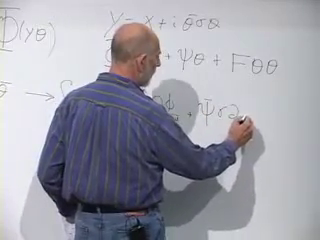
\includegraphics[width=0.76\textwidth]{lecture_09_figure_02.png}\lectureframe{00:27:36.000}\caption{스칼라, 페르미온, 보조장 항 위에 표시한 키랄 좌표와 성분 전개.}\end{figure}

\section{적분이 선택하는 것: \texorpdfstring{\(d^2\theta\)}{2} 적분}

상호작용과 질량은 초퍼텐셜인 정칙 함수 \(W(\Phi)\)에서 나온다.
\begin{equation}
S_W
=
\int d^4x
\left[
\int d^2\theta\,W(\Phi)
+\mathrm{h.c.}
\right].
\label{eq:l9-superpotential-action}
\end{equation}
키랄 표현에는 독립적인 \(\bar\theta\) 의존성이 없으므로 네 개의 반대칭 좌표 모두에 대해 적분하면 0이 된다. 대신 \(d^2\theta\) 적분은 그 표현의 \(\theta^2\) 성분을 선택한다.

일반 함수를 다루기 전에 계수 조합을 살펴보기 위해 \(W(\Phi)=\Phi^n\)라 하자. 다음 식에서
\begin{equation}
(\phi+\sqrt2\,\theta\psi+\theta^2F)^n,
\end{equation}
정확히 두 개의 \(\theta\)를 얻는 방법은 두 가지다. \(F\theta^2\) 하나를 택하거나 페르미온 인자를 두 개 택할 수 있다.

\begin{classroomqa}
\audiencequestion{하나의 \(F\theta^2\)를 택하고 나머지는 스칼라인 항은 몇 개 있나요? 스칼라는 \(n-1\)개 또는 \(n\)개인가요? \lecturetimestamp{00:31:33}}
\lecturerresponse{\(n\)개입니다. \(n\)개의 인자 가운데 어느 하나에서 \(F\theta^2\)를 택할 수 있고, 나머지 \(n-1\)개 인자는 \(\phi\)를 제공합니다. 따라서 기여항은 \(nF\phi^{n-1}\)입니다.}
\end{classroomqa}

\begin{classroomqa}
\audiencequestion{두 인자에서 페르미온 두 개를 얻는 방법은 몇 가지인가요? \lecturetimestamp{00:32:26}}
\lecturerresponse{순서 없는 선택은 \(\binom n2=n(n-1)/2\)가지입니다. 그라스만 수축이 이에 해당하는 \(\psi\psi\) 항을 정합니다.}
\end{classroomqa}

따라서 강의에서 계수를 생략한 표기법으로는 다음과 같다.
\begin{equation}
\int d^2\theta\,\Phi^n+\mathrm{h.c.}
\;\leadsto\;
nF\phi^{n-1}
-\frac{n(n-1)}{2}\phi^{n-2}\psi\psi
+\mathrm{h.c.}
\label{eq:l9-power-extraction}
\end{equation}
여기서 보인 마이너스 부호는 표준 정규화 전개와 그라스만 규약에서 나온다. 규약을 바꾸면 겉으로 드러나는 부호가 달라질 수 있다.

\begin{classroomqa}
\audiencequestion{\(\phi^n\)처럼 \(\theta\)가 하나도 없는 항은 어떻게 되었나요? \lecturetimestamp{00:33:10}}
\lecturerresponse{곱에는 들어 있지만 \(d^2\theta\)가 이를 버립니다. 화살표는 적분이 \(\theta^2\) 계수를 선택한다는 뜻이지, 전체 표현들이 같다는 뜻은 아닙니다.}
\end{classroomqa}

\begin{figure}[H]\centering
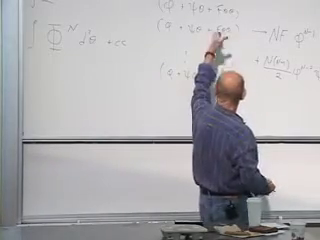
\includegraphics[width=0.82\textwidth]{lecture_09_figure_03.png}\lectureframe{00:33:38.000}\caption{반복되는 초장 인자들과, 두 \(\theta\) 성분을 등호가 아니라 추출한다는 뜻을 나타내는 함의 화살표.}\end{figure}

임의의 계수를 갖는 거듭제곱들을 모두 더하면 조합 계수가 도함수로 바뀐다.
\begin{equation}
\int d^2\theta\,W(\Phi)+\mathrm{h.c.}
\;\leadsto\;
F W'(\phi)
-\frac12 W''(\phi)\psi\psi
+\mathrm{h.c.}
\label{eq:l9-W-components}
\end{equation}

\begin{classroomqa}
\audiencequestion{\(\phi^{n-2}\) 대신 \(\phi^{n-1}\)가 페르미온 항에 들어가는 이유는 무엇인가요? \lecturetimestamp{00:36:32}}
\lecturerresponse{두 인자에서 이미 페르미온을 얻었으므로 스칼라 인자는 \(n-2\)개 남습니다. 계수는 2계 도함수 \(W''(\phi)\)의 절반입니다.}
\end{classroomqa}

페르미온 항은 중요하다. \(W''\)가 상수이면 질량을 주고, \(W''\)가 \(\phi\)에 의존하면 유카와 상호작용을 준다. 하지만 진공을 분석할 때는 보조장 항 \(FW'\)가 즉각적인 정보를 담고 있다.

\section{보조장 제거}

\(F\)을 포함하는 항들을 모으면 다음과 같다.
\begin{equation}
\mathcal L_F
=
F^\ast F
+F W'(\phi)
+F^\ast \overline{W'(\phi)}.
\label{eq:l9-LF}
\end{equation}
\(\partial_\mu F\)가 없으므로 완전한 오일러--라그랑주 방정식
\begin{equation}
\partial_\mu
\frac{\partial\mathcal L}{\partial(\partial_\mu F)}
-
\frac{\partial\mathcal L}{\partial F}
=0
\end{equation}
은 곧바로 대수 방정식으로 단순화된다. \(F\)와 \(F^\ast\)를 독립 변수로 취급하면
\begin{align}
\frac{\partial\mathcal L_F}{\partial F}
&=F^\ast+W'(\phi)=0,
&
\frac{\partial\mathcal L_F}{\partial F^\ast}
&=F+\overline{W'(\phi)}=0,
\label{eq:l9-F-eom}
\end{align}
를 얻고, 따라서
\begin{equation}
F^\ast=-W'(\phi),
\qquad
F=-\overline{W'(\phi)}.
\label{eq:l9-F-solution}
\end{equation}

\begin{figure}[H]\centering
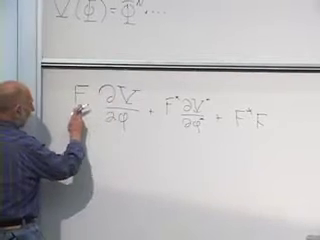
\includegraphics[width=0.82\textwidth]{lecture_09_figure_04.png}\lectureframe{00:39:40.000}\caption{가림 요소를 치운 뒤 보드에 함께 드러난 보조장 항 전체와 그 운동 방정식.}\end{figure}

\begin{classroomqa}
\audiencequestion{보드에 적힌 켤레장의 도함수가 아니라 \(\phi\)에 대해 미분해야 하지 않나요? \lecturetimestamp{00:41:21}}
\lecturerresponse{그렇습니다. 수정하면 ~\eqref{eq:l9-F-eom}에서 켤레 관계를 복원합니다. 즉 \(F^\ast=-W'(\phi)\)와 \(F=-\overline{W'(\phi)}\)입니다.}
\end{classroomqa}

~\eqref{eq:l9-LF}에 대입하면 다음을 얻는다.
\begin{equation}
\mathcal L_F\big|_{\mathrm{on\ shell}}
=-|W'(\phi)|^2.
\end{equation}
스칼라 라그랑지안은 운동 에너지에서 퍼텐셜 에너지를 뺀 형태이므로, 통상적인 스칼라 퍼텐셜은
\begin{equation}
\boxed{V(\phi,\phi^\ast)=|W'(\phi)|^2\ge0.}
\label{eq:l9-F-potential}
\end{equation}
이 \(V\)는 초퍼텐셜이 아니다. 정칙 초공간 함수에는 \(W\)를, 통상적인 퍼텐셜 에너지에는 \(V\)를 쓰겠다.

\subsection{바로 얻는 두 가지 예}

표준 규약에 따른 정규화를 사용하면
\begin{equation}
\begin{gathered}
W(\Phi)=\frac12m\Phi^2,\\
W'(\phi)=m\phi,
\qquad V=|m|^2|\phi|^2.
\end{gathered}
\label{eq:l9-quadratic-W}
\end{equation}
같은 항이 페르미온 질량 \(-\tfrac12m\psi\psi+\mathrm{h.c.}\)도 주므로, 초대칭이 깨지기 전에는 스칼라와 페르미온의 질량이 같다.

\begin{equation}
W(\Phi)=\frac{g}{3}\Phi^3,
\end{equation}을 가정하면
\begin{equation}
\begin{gathered}
W'(\phi)=g\phi^2,
\qquad V=|g|^2|\phi|^4,\\
\mathcal L_{\mathrm{Yukawa}}
=-g\phi\psi\psi+\mathrm{h.c.}
\end{gathered}
\label{eq:l9-cubic-W}
\end{equation}
사차 스칼라 꼭짓점은 두 스칼라의 산란을 나타내고, 유카와 항은 이에 대응하는 초대칭 짝이다.

\section{두 종류의 진공}

진공은 \(V\)가 최소인 상수 장 배치이며, 그 미분항은 사라진다. 식~\eqref{eq:l9-F-potential}이 음이 아니므로 가능한 경우는 두 가지다.

\subsection{에너지가 0인 최소점}

어떤 \(\phi_0\)가 다음을 만족하면
\begin{equation}
W'(\phi_0)=0,
\end{equation}
그러면
\begin{equation}
V(\phi_0)=0,
\qquad
\langle F\rangle=0.
\label{eq:l9-unbroken-F}
\end{equation}
진공은 초대칭을 보존한다. 이는 자화가 영인 경우에 해당한다. 어떤 보조장 성분도 초공간의 방향을 선택하지 않은 것이다.

\subsection{높아진 최소점}

최소점에서 방정식들
\begin{equation}
W'(\phi)=0
\label{eq:l9-F-flatness}
\end{equation}
을 동시에 만족하는 해가 없다면
\begin{equation}
V_{\min}>0,
\qquad
\langle F\rangle\neq0,
\label{eq:l9-broken-F}
\end{equation}
초대칭은 자발적으로 깨진다. 작용은 여전히 초대칭이지만, 가장 낮은 에너지 상태는 그렇지 않다.

\begin{figure}[H]\centering
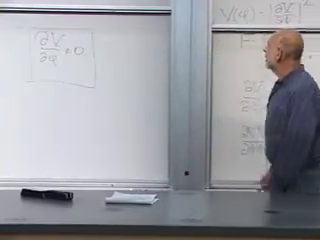
\includegraphics[width=0.88\textwidth]{lecture_09_figure_05.png}\lectureframe{00:52:09.960}\caption{양의 퍼텐셜, \(F\) 방정식, 진공 조건을 보드에 함께 제시하면서 대칭적인 방정식과 대칭을 따르지 않는 해를 구별한다.}\end{figure}

페르미온 변환을 통해 질서 매개변수에 관한 진술을 엄밀하게 표현할 수 있다.
\begin{equation}
\delta\psi_\alpha
=
i\sqrt2
(\sigma^\mu\bar\epsilon)_\alpha\partial_\mu\phi
+\sqrt2\,\epsilon_\alpha F.
\label{eq:l9-fermion-transformation}
\end{equation}
균일한 진공에서는 미분항이 사라진다. \(\langle F\rangle\neq0\)이면 초대칭 변환이 페르미온을 영이 아닌 상수만큼 이동시키므로 진공은 불변일 수 없다.\editorialnote{~\eqref{eq:l9-fermion-transformation}은 초장 성분들이 서로 변환된다는 강의의 설명을 명시적으로 보여 주는 표준 성분 형식이다.}

초대칭 대수에서도 같은 결론을 얻는다. 정지계에서는
\begin{equation}
\{Q_\alpha,Q_{\dot\alpha}^\dagger\}
=2\sigma^0_{\alpha\dot\alpha}H.
\end{equation}
진공 기대값을 취하면 에너지는 진공에 작용하는 초전하들의 노름의 합으로 표현된다.
\begin{equation}
E_0\ge0,
\qquad
E_0=0
\ \Longleftrightarrow\
Q_\alpha|0\rangle
=Q_{\dot\alpha}^\dagger|0\rangle=0.
\label{eq:l9-algebra-vacuum-energy}
\end{equation}
따라서 양의 진공 에너지와 자발적 초대칭 깨짐은 강체 초대칭에서 같은 진술의 두 측면이다.

\begin{center}
\begin{tikzpicture}[x=1.2cm,y=1.0cm,>=Latex]
  \draw[->] (-3,0) -- (-0.2,0) node[right] {\(\phi\)};
  \draw[->] (-2.8,-0.15) -- (-2.8,2.1) node[above] {\(V\)};
  \draw[thick,teal!75!black,domain=-2.5:-0.5,samples=60]
    plot (\x,{0.65*(\x+1.5)^2});
  \fill (-1.5,0) circle (2pt);
  \node[below] at (-1.5,0) {\(F=0\)};
  \draw[->] (0.4,0) -- (3.2,0) node[right] {\(\phi\)};
  \draw[->] (0.6,-0.15) -- (0.6,2.1) node[above] {\(V\)};
  \draw[thick,orange!85!black,domain=0.9:2.9,samples=60]
    plot (\x,{0.55*(\x-1.9)^2+0.65});
  \fill (1.9,0.65) circle (2pt);
  \draw[dashed] (0.6,0.65) -- (1.9,0.65);
  \node[below] at (1.9,0.65) {\(F\neq0\)};
\end{tikzpicture}
\end{center}

\editorialnote{간단한 예로 \(W=f\Phi\)를 들 수 있다. 이 경우 \(W'=f\)는 결코 사라지지 않으며 \(V=|f|^2\)이다. 이 한 장 모형에는 평탄한 스칼라 방향이 있다. 안정적인 \(F\)항 깨짐을 현실적으로 구현할 때는 보통 여러 카이랄 장을 사용하며, 오라페르타이형 숨은 부문이 그 예다.}

\section{초대칭 깨짐이 낳는 것}

\subsection{질량 분리}

이제 강자성체의 비유는 다시 스펙트럼에 관한 이야기로 이어진다. 약한 내부 자기장은 원자의 동일성을 없애지 않으면서 원자 준위를 분리한다. 마찬가지로 약하게 전달된 초대칭 깨짐 질서 매개변수는 그렇지 않았다면 한 초다중항에 속했을 보손과 페르미온을 분리한다.

\begin{classroomqa}
\audiencequestion{초대칭이 서로 변환시키며, 진공이 깨질 때 질량 축퇴를 잃는 입자는 무엇인가요? \lecturetimestamp{00:51:40}}
\lecturerresponse{보손과 페르미온입니다. 이들을 서로 연결하는 변환을 상태가 더 이상 따르지 않으면 질량이 같을 필요가 없습니다.}
\end{classroomqa}

분리는 \(\langle F\rangle\)만으로 생기는 것이 아니다. 깨짐을 가시 부문 장에 전달하는 결합에 달려 있다. 결합이 약하면 가시 입자들은 여전히 식별 가능하며, 질량 분리는 대통일 척도나 플랑크 척도보다 훨씬 작다. 결합이 강하다면, 엄청난 자기장 때문에 원자가 길게 늘어나 알아볼 수 없게 되는 상황에 비유할 수 있다.

\subsection{골드스티노}

일반적인 깨진 생성자에서는 \(J|0\rangle\)가 보손 골드스톤 상태를 준다. 초전하는 페르미온 생성자이며 보손 상태를 페르미온 상태로 바꾼다. 진공은 보손 상태로 간주되므로, 깨진 초전하는 에너지가 0인 페르미온 상태를 만든다.
\begin{equation}
Q_\alpha|0\rangle
\sim
|\widetilde G_\alpha,\mathbf k=0\rangle.
\label{eq:l9-goldstino}
\end{equation}
이 상태가 전파되는 형태는 무질량 바일 페르미온이며, 골드스톤 페르미온 또는 골드스티노라 부른다.

\begin{classroomqa}
\audiencequestion{초대칭 변환이 진공을 그대로 두지 않는다면 어떤 새로운 상태를 만들까요? \lecturetimestamp{00:53:24}}
\lecturerresponse{무질량 페르미온입니다. 일반적인 골드스톤 정리의 구조는 그대로지만, 페르미온 생성자가 보손 진공을 골드스티노로 바꿉니다.}
\end{classroomqa}

따라서 강체 초대칭의 자발적 깨짐에는 다음 두 가지 징후가 반드시 따른다.
\begin{equation}
\boxed{
V_{\min}>0
\qquad\text{and}\qquad
\text{a massless goldstino}.
}
\label{eq:l9-rigid-breaking-signatures}
\end{equation}

\section{숨은 부문}

원자와 강자성체를 두 부문으로 볼 수 있다. 강자성체에서는 질서 매개변수가 생기고, 원자는 거기서 전달된 장만 느낀다. 결합이 약하면 원자를 조작해도 마그논은 거의 들뜨지 않으므로 자기 매질에 직접 접근하기 어렵다. 이때 강자성체는 숨은 부문이지만, 작은 스펙트럼 분리를 통해 그 존재를 추론할 수 있다.

초대칭 모형 구축에서도 같은 용어를 사용한다. 숨은 부문의 추가 장들이 영이 아닌 \(F\)항 또는 \(D\)항 기댓값을 갖는다. 매개 메커니즘이라 불리는 상호작용은 그 깨짐을 가시 부문에 전달해 초대칭 짝들의 연성 질량을 만든다. 약한 전달은 훨씬 높은 근본 에너지 척도에서도 가시 이론이 근사적으로 초대칭을 유지하면서, 낮은 에너지에서는 보손--페르미온 사이에 정확한 축퇴가 나타나지 않을 수 있음을 설명해 준다.

이런 구성이 저절로 되는 것은 아니다. 추가 장, 안정적인 깨짐 진공, 제어 가능한 매개 메커니즘이 필요하다. 그래서 강의에서는 현실적인 초대칭 깨짐을 최소 모형에서 필연적으로 따라 나오는 단일 결과가 아니라 복잡하고 다소 인위적인 구성이라고 설명한다.

\section{중력은 두 가지 징후를 모두 바꾼다}

\subsection{진공 에너지가 중력의 원천이 된다}

중력이 없으면 모든 에너지에 상수를 더해도 비중력 실험은 달라지지 않는다. 중력이 있으면 진공 에너지 밀도는 우주상수로 아인슈타인 방정식에 들어간다. 양의 \(V_{\min}\)는 가속 팽창을 일으킨다. 그 척도가 초대칭 짝의 질량에 필요한 입자물리학 척도에 가깝다면, 그에 따른 곡률은 관측된 값보다 엄청나게 커진다.

\begin{classroomqa}
\audiencequestion{중력을 포함하면 양의 영이 아닌 진공 에너지는 우주에 어떤 영향을 미치나요? \lecturetimestamp{01:00:40}}
\lecturerresponse{우주상수로 작용해 가속 팽창을 일으킵니다. 보통의 입자물리학 에너지 척도에서는 그 효과가 도저히 감당할 수 없을 만큼 큽니다.}
\end{classroomqa}

국소 초대칭, 즉 초중력은 양의 제곱합 공식을 바꾼다. 참고로 표준 \(N=1\) \(F\)항 퍼텐셜은 다음과 같다.
\begin{equation}
\begin{aligned}
V_F={}&e^{K/M_P^2}
\left(
K^{i\bar j}D_iW\,D_{\bar j}\overline W
-\frac{3|W|^2}{M_P^2}
\right),\\
D_iW={}&\partial_iW+\frac{\partial_iK}{M_P^2}W.
\end{aligned}
\label{eq:l9-sugra-potential}
\end{equation}
음의 항이 있으므로 초대칭 깨짐에서 나온 양의 에너지는 원리상 일부 상쇄될 수 있다. 나머지는 작은 우주상수일 수 있다.

\editorialnote{강의에서는 의도적으로 개략적인 보정항만 제시하며 플랑크 질량의 위치에도 의문을 제기한다. ~\eqref{eq:l9-sugra-potential}은 켈러 퍼텐셜 \(K\)을 갖는 키랄 다중항에 대한 표준 공식을 기록한다. 게이지 \(D\)항을 더하면 음이 아닌 기여항이 추가된다. 관측된 값이 왜 그토록 작은지는 설명하지 않으며, 이는 여전히 우주상수 문제로 남아 있다.}

\subsection{초힉스 메커니즘}

두 번째 중력 효과는 편극 상태를 세어 보면 가장 쉽게 이해할 수 있다. 질량을 가진 스핀 \(j\) 입자는 정지계에서 \(2j+1\)개의 스핀 상태를 갖는다.

\begin{classroomqa}
\audiencequestion{질량이 있는 스핀\(j\)입자에는 스핀 상태가 몇 개 있나요? \lecturetimestamp{01:05:16}}
\lecturerresponse{\(2j+1\). 특히 질량이 있는 스핀 일 입자에는 상태가 세 개 있는 반면, 질량이 없는 게이지 보손에는 헬리시티 \(+1\)와 \(-1\)만 있습니다.}
\end{classroomqa}

이 차이는 운동학적인 것이다. 질량이 있는 입자는 정지계로 로런츠 변환한 뒤 스핀 방향을 유지한 채 새 방향으로 보낼 수 있으므로, 모든 투영 상태가 존재해야 한다. 무질량 입자는 앞질러 가거나 정지 상태로 만들 수 없다. 따라서 양 끝의 두 헬리시티만 가질 수 있다.

전자기약 게이지장에서는
\begin{equation}
\underbrace{(+1,-1)}_{\text{massless vector}}
+
\underbrace{(0)}_{\text{Goldstone}}
\longrightarrow
\underbrace{(+1,0,-1)}_{\text{massive vector}}.
\label{eq:l9-higgs-count}
\end{equation}

\begin{classroomqa}
\audiencequestion{질량이 있는 \(W\) 또는 \(Z\) 보손의 종방향 편극은 어디서 오나요? \lecturetimestamp{01:08:50}}
\lecturerresponse{골드스톤 보손에서 옵니다. 게이지장에 흡수되어 질량이 있는 스핀 1 표현의 세 상태를 완성합니다.}
\end{classroomqa}

중력에는 무질량 스핀 2 중력자가 있다. 그 초대칭 짝은 무질량 스핀 \(\tfrac32\) 중력자이다.

\begin{classroomqa}
\audiencequestion{중력자의 스핀은 얼마이며, 따라서 그 초대칭 짝의 스핀은 얼마인가요? \lecturetimestamp{01:10:24}}
\lecturerresponse{중력자의 스핀은 \(2\)이고, 페르미온 짝은 스핀이 절반만큼 달라서 \(3/2\)입니다.}
\end{classroomqa}

무질량 중력자는 헬리시티 \(\pm\tfrac32\)를 갖지만, 질량이 있는 중력자는 \(\pm\tfrac12\)도 가져야 한다. 골드스티노가 바로 이 빠진 상태들을 제공한다.
\begin{equation}
\begin{gathered}
\underbrace{\left(+\frac32,-\frac32\right)}_{\text{massless gravitino}}
\oplus
\underbrace{\left(+\frac12,-\frac12\right)}_{\text{goldstino}}\\
\Downarrow\\
\underbrace{\left(+\frac32,+\frac12,-\frac12,-\frac32\right)}_{\text{massive gravitino}}.
\end{gathered}
\label{eq:l9-super-higgs}
\end{equation}
이것이 초힉스 메커니즘이다. 초대칭이 국소 대칭이면 골드스티노는 흡수되어 더 이상 독립적인 무질량 입자로 나타나지 않는다. 그 결과 생기는 중력자는 중력 상호작용을 하므로 생성하기도 그만큼 어렵다.

\section{주제 전환: 왜 \texorpdfstring{\(SU(5)\)}{SU(5)}인가?}

이제 초대칭 형식론에서 대통일로 넘어간다. 표준 모형 게이지 군은 다음과 같다.
\begin{equation}
G_{\mathrm{SM}}
=SU(3)_c\times SU(2)_L\times U(1)_Y.
\label{eq:l9-sm-group}
\end{equation}
세 인자는 각각 색, 약아이소스핀, 약한 초전하를 조직한다. 대통일에서 묻는 것은 이 곱군이 더 큰 단순군의 잔존 부분군인지, 즉 서로 분리된 것처럼 보이는 입자 다중항과 게이지 힘이 하나의 구조를 이루는지다. 여기서 다룰 최소 후보는 \(SU(5)\)이다.

\subsection{군 원소와 생성자}

\(U\in SU(N)\)에 대해
\begin{equation}
U^\dagger U=\mathbf1,
\qquad
\det U=1.
\label{eq:l9-SUN-def}
\end{equation}
첫 번째 조건은 유니터리성을 뜻하고, 두 번째 조건은 ‘특수’라는 말의 의미다. 무한소 원소를 다음과 같이 쓰자.
\begin{equation}
U=\mathbf1+i\epsilon G+\mathcal O(\epsilon^2).
\label{eq:l9-infinitesimal-U}
\end{equation}
유니터리성으로부터
\begin{equation}
G^\dagger=G,
\end{equation}
그리고
\begin{equation}
\det e^{i\epsilon G}
=e^{i\epsilon\operatorname{tr}G}=1
\end{equation}
로부터
\begin{equation}
\operatorname{tr}G=0.
\end{equation}
가 따라온다. 따라서 생성자는 자취가 영인 에르미트 행렬이다.

\(N\times N\) 에르미트 행렬에는 실수 매개변수가 \(N^2\)개 있다. 실수 대각 성분이 \(N\)개이고 비대각 성분이 복소수 \(N(N-1)/2\)개다. 무자취 조건으로 하나가 줄어든다. 따라서
\begin{equation}
\dim SU(N)=N^2-1,
\qquad
\dim SU(5)=24.
\label{eq:l9-SU5-dimension}
\end{equation}
참고로 \(SU(2)\)에는 파울리 생성자가 세 개 있고, \(SU(3)\)에는 색 생성자가 여덟 개 있다.

\section{\texorpdfstring{\(SU(5)\)}{SU(5)} 내부의 표준 모형 블록}

5차원 공간을 약한 상호작용의 2차원 블록과 색의 3차원 블록으로 나눈다.
\begin{equation}
\mathbf5=\mathbf2\oplus\mathbf3.
\end{equation}
포함된 생성자는 다음 형태다.
\begin{align}
T^a_L
&=
\begin{pmatrix}
\tfrac12\tau^a&0\\
0&0_{3\times3}
\end{pmatrix},
&& a=1,2,3,
\label{eq:l9-SU2-block}\\
T^A_c
&=
\begin{pmatrix}
0_{2\times2}&0\\
0&\tfrac12\lambda^A
\end{pmatrix},
&& A=1,\ldots,8.
\label{eq:l9-SU3-block}
\end{align}
파울리 행렬 \(\tau^a\)은 약한 상호작용의 \(SU(2)\)를 생성하고, 겔만 행렬 \(\lambda^A\)은 색의 \(SU(3)\)를 생성한다. 두 블록은 겹치지 않으므로 두 부분군은 서로 가환한다.

추가 대각 생성자 하나는 각 블록 안에서 항등행렬에 비례하므로 두 블록 모두와 교환한다. 기본 표현에서 편리한 이중화 하이퍼전하 규약을 하나 택하면
\begin{equation}
T_Y^{(\mathbf5)}=
\operatorname{diag}
\left(
1,1,-\frac23,-\frac23,-\frac23
\right).
\label{eq:l9-hypercharge-generator}
\end{equation}
그 자취는 영이다.
\begin{equation}
1+1-3\left(\frac23\right)=0.
\end{equation}
켤레 물질 표현에서는 고윳값의 부호가 반대다.
\begin{equation}
Y_{\overline{\mathbf5}}
=
\operatorname{diag}
\left(
-1,-1,\frac23,\frac23,\frac23
\right),
\label{eq:l9-fivebar-hypercharge}
\end{equation}
이 값들이 강의에서 물질 열에 적힌 값이다. 전체 부호와 정규화는 관례에 따른다. 여기서는 표준 모형 규약
\begin{equation}
Q=T_3+\frac{Y}{2}.
\label{eq:l9-charge}
\end{equation}
을 사용한다. 식들~\eqref{eq:l9-SU2-block}--\eqref{eq:l9-hypercharge-generator}은 다음을 보여 준다.
\begin{equation}
SU(3)_c\times SU(2)_L\times U(1)_Y
\subset SU(5).
\end{equation}

약한 상호작용 생성자 3개, 색 생성자 8개, 초전하 생성자 1개를 합하면 \(12\)\(24\)개의 \(SU(5)\) 생성자가 된다.\editorialnote{나머지 12개는 비대각 \(2\times3\) 및 \(3\times2\) 블록에 놓인다. 이 생성자들의 게이지 보손은 쿼크형 성분과 렙톤형 성분을 서로 바꾸며, 이것이 후속 강의에서 다룰 바리온수 및 렙톤수 변화 상호작용의 구조적 기원이다.}

\begin{classroomqa}
\audiencequestion{익숙한 부분군 생성자에는 어떤 게이지 입자들이 대응하는가? \lecturetimestamp{01:31:05}}
\lecturerresponse{\(SU(3)\) 생성자 8개는 글루온 8개를 준다. \(SU(2)\) 생성자 3개는 약한 게이지장을 주며, 이들은 전약 혼합을 거쳐 \(W^\pm\)와 \(Z\)-광자 계의 일부가 된다. \(U(1)\) 장은 다른 중성 조합을 제공한다.}
\end{classroomqa}

\section{왼손 성분으로 나타낸 한 세대}

첫 번째 세대를 살펴보자. 뮤온/참/기묘 세대와 타우/톱/아래 세대에서도 같은 패턴이 반복된다. 서로 독립인 바일 장을 모두 왼손 성분으로 세는 것이 가장 간결하다. 오른손 입자는 이에 대응하는 왼손 전하켤레장으로 나타낸다:
\begin{equation}
Q_L=(u_L,d_L),\quad
L_L=(\nu_{eL},e_L),\quad
u^c_L,\quad d^c_L,\quad e^c_L.
\end{equation}
각 장의 중복도는 다음과 같다.
\begin{equation}
\underbrace{6}_{Q_L}
+
\underbrace{2}_{L_L}
+
\underbrace{3}_{u^c_L}
+
\underbrace{3}_{d^c_L}
+
\underbrace{1}_{e^c_L}
=15.
\label{eq:l9-fifteen-fields}
\end{equation}

\editorialnote{최소 표준 모형에는 독립적인 오른손 중성미자 바일 장이 없으므로, 그 수는 \(15\)이다. 이 셈만으로 중성미자가 마요라나 입자라고 주장하는 것은 아니다. 단일항 \(\nu^c_L\)를 더하면 장은 \(16\)개가 되며, 현재의 \(SU(5)\) 구성 범위를 넘어 \(SO(10)\)로 자연스럽게 이어진다.}

5차원 다중항의 첫 두 자리는 색을 띠지 않는 약한 이중항 성분이, 마지막 세 자리는 색을 띠는 약한 단일항 성분이 차지해야 한다.

\begin{classroomqa}
\audiencequestion{제안된 열에는 5개가 아니라 6개 장이 들어가는가? \lecturetimestamp{01:36:14}}
\lecturerresponse{아니다. 첫 번째 풀이에서 적었던 위 쿼크는 지운다. 이 열은 중성미자, 전자, 그리고 아래반쿼크의 색 상태 3개로 이루어지므로 모두 5개 성분이다.}
\end{classroomqa}

그러면 다음과 같다.
\begin{equation}
\overline{\mathbf5}
=
\begin{pmatrix}
\nu_{eL}\\
e_L\\
d^c_{rL}\\
d^c_{gL}\\
d^c_{bL}
\end{pmatrix}.
\label{eq:l9-fivebar}
\end{equation}\editorialnote{강의에서는 처음에 이것을 단순히 5차원 다중항이라고 부른다. 표준적인 왼손 성분만 쓰는 \(SU(5)\) 표기에서 색과 초전하의 배정은 이것이 켤레 표현 \(\overline{\mathbf5}\)임을 나타낸다.}
처음 두 성분은 \(SU(2)_L\) 아래에서 변환하지만 색을 띠지 않는다. 마지막 세 성분은 색에 대해 반삼중항으로 변환하며 약한 상호작용의 단일항이다.

\begin{classroomqa}
\audiencequestion{모든 장을 왼손 성분으로 썼을 때, 어떤 쿼크가 색을 띠지만 약한 \(SU(2)_L\) 양자수는 갖지 않는가? \lecturetimestamp{01:40:13}}
\lecturerresponse{오른손 쿼크의 전하켤레장이다. 이 5성분 다중항에서는 전하를 따져 보면 아래반쿼크 장 세 개 \(d^c_{r,g,b}\)가 해당한다.}
\end{classroomqa}

식~\eqref{eq:l9-fivebar}의 전하를 모두 더하면 0이다:
\begin{equation}
0-1+\frac13+\frac13+\frac13=0.
\label{eq:l9-fivebar-charge-sum}
\end{equation}
전하 연산자는 \(SU(5)\) 생성자의 무자취 조합이므로 그래야 한다.

\begin{classroomqa}
\audiencequestion{왜 반다운 쿼크가 반업 쿼크가 아니라 세 개의 색 자리를 차지하나요? \lecturetimestamp{01:43:38}}
\lecturerresponse{중성미자와 전자의 총 전하는 \(-1\)입니다. 세 가지 색의 반다운 쿼크가 기여하는 전하는 \(+1\)이므로, 대각합은 0이 됩니다. 반업 쿼크 세 개를 두면 전체 전하가 맞지 않습니다.}
\end{classroomqa}

남은 왼손 성분 장 10개는 다음과 같다.
\begin{equation}
Q_L\;(6)
\oplus
u^c_L\;(3)
\oplus
e^c_L\;(1),
\end{equation}
이들은 반대칭 2계 표현에 정확히 들어맞는다.
\begin{equation}
\mathbf{10}\cong\wedge^2\mathbf5,
\qquad
\dim\wedge^2\mathbf5=\binom52=10.
\label{eq:l9-ten-preview}
\end{equation}
이 장들을 구체적으로 배치하는 일은 다음 강의에서 다룬다. 모든 표준 모형 세대에서 성립하는 이 수치적 일치
\begin{equation}
\overline{\mathbf5}\oplus\mathbf{10}
\end{equation}
는 \(SU(5)\) 발상이 임의로 이름만 바꾸어 붙인 것이 아님을 보여 주는 첫 번째 놀라운 증거다.

\begin{classroomqa}
\audiencequestion{5와 10이 서로 다른 표현이라면, 그 입자들은 서로 상호작용할 수 없다는 뜻인가요? \lecturetimestamp{01:46:14}}
\lecturerresponse{아닙니다. 군 변환은 각 기약표현 안에서 작용하므로, 5에 속한 성분을 10에 속한 성분으로 직접 변환하지는 않습니다. 그렇더라도 두 집합은 공통의 게이지 보손을 방출하고 흡수함으로써 상호작용할 수 있으며, 힉스 결합도 두 집합의 장을 서로 연결할 수 있습니다.}
\end{classroomqa}

\section{조망}

이 강의에서는 매우 다른 규모에 걸쳐 하나의 패턴을 따라왔다. 회전 대칭성은 원자 준위를 축퇴시키고, 자기 배경은 그 축퇴를 깨뜨린다. 강자성체는 바탕이 되는 법칙의 대칭성을 유지하면서 그러한 배경을 만들며, 갭이 없는 마그논은 비대칭성이 진공에 있음을 드러낸다. 손지기 초대칭 이론에서는 보조장의 기대값이 질서 매개변수 역할을 한다:
\begin{equation}
\begin{aligned}
\langle F\rangle=0
&\quad\Longleftrightarrow\quad
\text{unbroken supersymmetry},\\
\langle F\rangle\neq0
&\quad\Longrightarrow\quad
\text{spontaneous breaking}.
\end{aligned}
\end{equation}
강직한 초대칭에서 깨진 진공은 양의 에너지를 가지며, 초다중항의 질량 축퇴를 깨고, 골드스티노를 만든다. 약한 매개는 숨은 섹터를 도입할 동기를 제공한다. 중력은 진공 에너지를 우주론적 문제로 만들고, 골드스티노를 흡수하여 질량을 가진 중력자를 만든다.

마지막의 \(SU(5)\) 구성은 새로운 질문을 던지기 시작할 뿐, 답을 완성하지는 않는다. 무자취 에르미트 \(5\times5\) 생성자 안에는 표준 모형 블록이 들어 있으며, 처음 다섯 물질장은 정확히 다음과 같이 들어맞는다.
\((\nu_e,e^-,d^c_r,d^c_g,d^c_b)\). 나머지 열 개는 반대칭 표현에 들어갈 차례다. 이 미완의 맞춤이 바로 대통일이 본격적으로 시작되는 지점이다.

\chapter{\texorpdfstring{\(SU(5)\)}{5} 다중항, 렙토쿼크 게이지 보손과 양성자 붕괴}

\lectureoverview{표준 모형의 군을 \(SU(5)\)에 포함하면 대통일이 구체적인 형태를 갖는다. 이 말의 뜻을 이해하기 위해 먼저 필요한 표현론을 살펴보자. 기본 표현 \(N\)과 그 켤레 표현 \(\overline N\), 텐서곱, 대칭 및 반대칭 텐서, 그리고 수반 표현이 그것이다. 그러면 표준 모형의 한 세대가 놀라울 만큼 간결한 조합 \(\overline{\mathbf 5}\oplus\mathbf{10}\)으로 묶인다. 이 구성을 아름답게 만드는 대칭성은 쿼크를 렙톤으로 바꾸는 색전하 게이지 보손도 요구한다. 이 보손의 교환은 양성자 붕괴를 허용하므로 통일 에너지 척도는 \(10^{15}\)--\(10^{16}\,\mathrm{GeV}\) 부근이어야 한다. 게이지 결합상수의 에너지에 따른 변화도 비슷한 척도를 가리킨다. 마지막에 초대칭을 다시 살펴보는 이유는 초대칭을 포함하면 결합상수들이 만나는 값이 수치상 훨씬 더 정확하게 일치하기 때문이다.}

\section{군 표현부터 시작하는 이유}

대통일 이론은 여러 가지가 제안되어 있다. 이론들을 두루 살펴보는 대신, 한 가지 사례를 뜯어보며 세 가지를 묻겠다. 무엇이 이 이론을 성립하게 하는가? 어떤 새 입자들이 필요한가? 실험은 이 이론을 어디에서 위태롭게 하는가? 여기서 다룰 군은 \(SU(5)\)이며, 그 구조의 핵심은 다음 포함 관계다.
\begin{equation}
SU(3)_c\times SU(2)_L\times U(1)_Y
\subset SU(5).
\label{eq:l10-sm-embedding}
\end{equation}
여기서 \(SU(3)_c\)은 색에, \(SU(2)_L\)은 약한 아이소스핀에, \(U(1)_Y\)은 약한 하이퍼전하에 작용한다.

초대칭은 이 구성의 전제가 아니다. 초대칭이 대통일을 논리적으로 함의하지도 않고, 대통일이 초대칭을 함의하지도 않는다. 이 강의에서 둘의 연결고리는 수치적이다. 초짝입자 스펙트럼을 재규격화군 계산에 포함하면 세 게이지 결합상수가 공통값에 더 정확하게 가까워진다.

대칭 변환이 서로 섞는 입자들은 대칭군의 표현을 이룬다. 따라서 통일된 입자 다중항을 분류하려면 먼저 표현론을 조금 살펴볼 필요가 있다.

\subsection{익숙한 \texorpdfstring{\(SU(2)\)}{2} 예}

보통 각운동량과 관련된 \(SU(2)\)은 3차원 공간의 회전과 밀접하게 연관되어 있다. 더 정확히 말하면, \(SU(2)\)은 \(SO(3)\)의 이중 덮개다. 그 기약 표현은 다음과 같이 표기한다.
\begin{equation}
j=0,\frac12,1,\frac32,\ldots,
\qquad
\dim(j)=2j+1.
\label{eq:l10-su2-spins}
\end{equation}
따라서 스칼라는 단일항이고, 스핀 \(\tfrac12\) 입자는 이중항이며, 스핀 1 입자는 삼중항이다. 약한 상호작용의 군 \(SU(2)_L\)은 물리적으로는 다른 대칭이지만, 추상적인 군론은 같다.

\section{기본 표현과 그 켤레 표현}

\(SU(N)\)에서 기본 표현은 복소수 \(N\)성분 열벡터들의 공간이다.
\begin{equation}
\psi=
\begin{pmatrix}
\psi_1\\
\psi_2\\
\vdots\\
\psi_N
\end{pmatrix},
\qquad
\psi'_i=U_i{}^j\psi_j,
\qquad
U\in SU(N).
\label{eq:l10-defining}
\end{equation}
이를 기본 표현이라고 하거나 간단히 \(\mathbf N\)라고 부른다. 행렬 \(U\)은 \(N\times N\) 행렬이며, 이 행렬이 작용하는 벡터 공간의 차원은 \(N\)이다.

복소켤레를 취하면 또 하나의 \(N\)차원 표현을 얻는다.
\begin{equation}
\psi_i^*\longmapsto U_i{}^{j*}\psi_j^*,
\label{eq:l10-conjugate}
\end{equation}
이를 \(\overline{\mathbf N}\)로 표기한다. \(N>2\)에서는 기본 표현과 켤레 표현이 동등하지 않다. 어느 쪽을 입자 표현으로, 어느 쪽을 반입자 표현으로 부를지는 바꿀 수 있지만, 관례를 정한 뒤에는 일관되게 유지해야 한다.

\begin{classroomqa}\audiencequestion{\(N\)가 \(SU(N)\)에서 \(N\)이 짝수인지 홀수인지에 따라 달라지나요? 행렬을 가리키는 건가요? \lecturetimestamp{00:07:33}}
\lecturerresponse{여기에는 짝수--홀수에 따른 제한이 없습니다. \(N\)은 기본 행렬의 크기이자 기본 표현의 차원이기도 합니다. \(\mathbf N\)와 \(\overline{\mathbf N}\)은 둘 다 그 차원을 갖습니다.}
\end{classroomqa}

반입자의 반입자는 원래 입자다. 그러므로 \(\mathbf N\)와 \(\overline{\mathbf N}\)의 이름을 서로 바꾸는 것은 물리학이 아니라 관례를 바꾸는 일이다.

\section{텐서곱과 기약성}

한 물체가 \(N\)개의 내부 상태를 가질 수 있고, 다른 물체도 독립적으로 똑같은 수의 상태를 가질 수 있다고 하자. 위치, 운동량, 스핀 및 이 \(SU(N)\) 표지 외의 모든 양자수를 무시하면 두 물체의 쌍은
\begin{equation}
N\times N=N^2
\label{eq:l10-product-count}
\end{equation}
개의 상태를 갖는다. 첫 번째 물체가 상태 \(\psi_i\)에 있고 두 번째 물체가 상태 \(\phi_j\)에 있다면, 그 곱은 다음과 같이 쓸 수 있다.
\begin{equation}
\Psi_{ij}=\psi_i\phi_j,
\qquad
\Psi'_{ij}=U_i{}^kU_j{}^\ell\Psi_{k\ell}.
\label{eq:l10-tensor-transform}
\end{equation}
이것이 텐서곱 \(\mathbf N\otimes\mathbf N\)이다.

\begin{classroomqa}\audiencequestion{왜 답이 \(N^2\)인가요? \(N^2-1\)이 아닌가요? 두 입자가 같은 내부 표지를 갖도록 허용하면 배타 원리를 위반하지 않나요? \lecturetimestamp{00:10:22}}
\lecturerresponse{여기서는 두 자리가 구별된다. 한 물체는 한 위치에 고정되어 있고 다른 물체는 다른 위치에 있다. 파울리 원리는 위치를 포함한 완전한 양자 상태에 제약을 가한다. 이 원리가 \(N^2\)개의 내부 표지 조합을 제거하지는 않는다. \(N^2-1\)이라는 수는 뒤에서 다른 곱에 무흔적 조건을 적용할 때 나온다.}
\end{classroomqa}

차원 \(N^2\)인 곱 표현은 일반적으로 가약이다. 표현에 군의 작용을 받아도 그 안에 머무는 진부분공간이 있으면 그 표현을 가약이라 한다. 이런 불변 부분공간을 분리해 더 작은 표현으로 다룰 수 있다. 그러한 진부분공간이 하나도 없으면 그 표현은 기약이다.

\subsection{대칭 텐서와 반대칭 텐서}

모든 2계 텐서는 다음 두 부분으로 유일하게 분해된다.
\begin{align}
\Psi_{ij}
&=\Psi^{(S)}_{ij}+\Psi^{(A)}_{ij},\\
\Psi^{(S)}_{ij}
&=\frac12(\Psi_{ij}+\Psi_{ji}),\\
\Psi^{(A)}_{ij}
&=\frac12(\Psi_{ij}-\Psi_{ji}).
\label{eq:l10-sym-anti}
\end{align}
두 부분은 다음 성질을 만족한다.
\begin{equation}
\Psi^{(S)}_{ij}=\Psi^{(S)}_{ji},
\qquad
\Psi^{(A)}_{ij}=-\Psi^{(A)}_{ji}.
\end{equation}
식~\eqref{eq:l10-tensor-transform}은 각각의 조건을 보존하므로 군 변환으로 대칭 부문과 반대칭 부문이 서로 섞이지 않는다.

\editorialnote{강의에서는 일반적인 경우의 셈을 연습문제로 남겨 두었다. 대칭 및 반대칭 부분공간의 차원은 각각 \(N(N+1)/2\)와 \(N(N-1)/2\)이며, 두 차원을 더하면 \(N^2\)이다.}

\begin{figure}[htbp]\centering
\includegraphics[width=0.78\textwidth]{lecture_10_figure_02.png}\lectureframe{00:17:57.500}\caption{스핀 \(\tfrac12\) 상태 두 개를 대칭 상태 세 개와 반대칭 상태 하나로 완전히 분해한 판서.}\label{fig:l10-spin-decomposition}\end{figure}

\(SU(2)\)의 기본 이중항에 대해,
\begin{equation}
\mathbf2\otimes\mathbf2=\mathbf3_S\oplus\mathbf1_A.
\label{eq:l10-two-two}
\end{equation}
두 기저 상태를 \(u\)와 \(d\)로 쓰면, 대칭 삼중항은 다음과 같다.
\begin{align}
\ket{1,1}&=\ket{uu},\\
\ket{1,0}&=\frac{1}{\sqrt2}\bigl(\ket{ud}+\ket{du}\bigr),\\
\ket{1,-1}&=\ket{dd},
\end{align}
반면 반대칭 단일항은 다음과 같다.
\begin{equation}
\ket{0,0}
=\frac{1}{\sqrt2}\bigl(\ket{ud}-\ket{du}\bigr).
\end{equation}
이것은 스핀 \(\tfrac12\) 각운동량 두 개를 더하는 익숙한 결과다. 원래의 네 상태가 스핀 1과 스핀 0으로 재구성된다.

\section{입자와 반입자: 수반 표현}

이제 기본 표현과 그 켤레 표현을 결합하자. 곱에는 여전히 \(N^2\)개의 성분이 있지만, 행렬처럼 변환한다.
\begin{equation}
M_i{}^j\in\mathbf N\otimes\overline{\mathbf N},
\qquad
M\longmapsto U M U^\dagger.
\label{eq:l10-matrix-transform}
\end{equation}
\(\mathbf N\otimes\mathbf N\)과 달리 기본 표현 지표 하나와 반기본 표현 지표 하나 사이에는 의미 있는 교환 대칭이 없다. 대신 자연스러운 분해는 다음과 같다.
\begin{equation}
M
=
\frac{\operatorname{tr}M}{N}\,\mathbf1_N
+
\left(M-\frac{\operatorname{tr}M}{N}\,\mathbf1_N\right).
\label{eq:l10-trace-split}
\end{equation}
첫 번째 항은 단일항이고, 무흔적 부분은 수반 표현이다.
\begin{equation}
\mathbf N\otimes\overline{\mathbf N}
=\mathbf1\oplus\mathbf{Adj},
\qquad
\dim\mathbf{Adj}=N^2-1.
\label{eq:l10-adjoint}
\end{equation}

\begin{figure}[htbp]\centering
\includegraphics[width=0.67\textwidth]{lecture_10_figure_04.png}\lectureframe{00:23:47.500}\caption{\(\mathbf N\otimes\overline{\mathbf N}\)의 무흔적 성분 \(N^2-1\)개가 수반 표현을 이룬다는 판서의 결론.}\label{fig:l10-adjoint}\end{figure}

\(SU(3)\)에서는 익숙한 팔중항을 얻는다.
\begin{equation}
\mathbf3\otimes\overline{\mathbf3}
=\mathbf8\oplus\mathbf1,
\end{equation}
8개의 글루온은 수반 표현으로 변환한다. \(SU(2)\)에서는 수반 표현의 차원이 3이며 스핀 1처럼 변환한다.

\section{표준 모형의 한 세대}

관측된 세대는 세 개지만, \(SU(5)\)은 각 세대에 같은 구성을 별도로 적용한다. 세 복사본이 존재하는 이유까지 설명하지는 않는다. 따라서 첫 번째 세대에 초점을 맞추자.

모든 장은 왼손잡이 바일 장으로 쓰겠다. 오른손잡이 페르미온은 왼손잡이 전하켤레 장으로 나타낸다.
\begin{equation}
u^c_L,\qquad d^c_L,\qquad e^c_L.
\label{eq:l10-left-handed-bookkeeping}
\end{equation}
위첨자 \(c\)은 전하켤레를 뜻한다. 예를 들어 \(d^c_L\)은 전기 전하가 \(+\tfrac13\)인 왼손잡이 반다운 쿼크 장이다.

표준적인 \(SU(5)\) 표기법에서 왼손잡이 장 15개 중 다섯 개는 다음 표현에 들어간다.
\begin{equation}
\overline{\mathbf5}
=
\begin{pmatrix}
\nu_{eL}\\
e_L\\
d^c_{rL}\\
d^c_{gL}\\
d^c_{bL}
\end{pmatrix}.
\label{eq:l10-fivebar}
\end{equation}
약한 상호작용의 2차원 블록을 먼저 쓰고 색의 3차원 블록을 뒤에 쓰도록 순서를 정했다. 약한 상호작용의 변환은 앞의 두 성분을 서로 섞고, 색 변환은 마지막 세 성분을 서로 섞는다. 비대각 \(SU(5)\) 생성자는 두 블록을 연결한다.

\editorialnote{강의에서는 식~\eqref{eq:l10-fivebar}의 열벡터를 \(\mathbf5\)라고 부르고, 뒤에서는 반대칭 다중항을 \(\overline{\mathbf{10}}\)라고 부른다. 이는 모든 표현을 전역적으로 켤레화한 관례다. 여기서는 현대 표준 관례 \(\overline{\mathbf5}\oplus\mathbf{10}\)를 사용한다. 모든 표현을 켤레화하면 물리학은 그대로 둔 채 강의의 명칭을 재현할 수 있다.}

최소 모형에서 첫 세대의 전체 구성은 다음과 같다.
\begin{equation}
\begin{gathered}
\underbrace{Q_L=(u_L,d_L)}_{6}
\oplus
\underbrace{L_L=(\nu_{eL},e_L)}_{2},\\
\underbrace{u^c_L}_{3}
\oplus
\underbrace{d^c_L}_{3}
\oplus
\underbrace{e^c_L}_{1},\\
6+2+3+3+1=15.
\end{gathered}
\label{eq:l10-fifteen}
\end{equation}
최소 표준 모형에는 독립적인 \(\nu^c_L\)가 없으므로 재규격화 가능한 중성미자 질량을 줄 수 없다. 중성미자 진동은 이 최소 모형의 설명이 불완전함을 보여 준다. 자연에는 영이 아닌 작은 중성미자 질량이 있으며, 이를 설명하려면 모형을 확장해야 한다.

\begin{classroomqa}\audiencequestion{페르미온 질량이 왼손잡이 상태를 오른손잡이 상태로 바꿀 때, 입자도 반입자로 바뀌나요? \lecturetimestamp{00:34:00}}
\lecturerresponse{아니다. 전자 질량은 왼손잡이 전자와 전기 전하가 같은 오른손잡이 전자를 연결한다. 모든 장을 왼손잡이로 쓰는 표기법에서는 두 번째 장을 \(e^c_L\)로 나타내지만, 4성분 입자는 여전히 전자다. 입자와 반입자를 동일시하는 마요라나 질량을 가질 수 있는 것은 중성 장뿐이다.}
\end{classroomqa}

\section{다중항에서 드러나는 게이지 보손}

게이지 대칭의 각 생성자에는 그에 대응하는 게이지 장이 있다. 식~\eqref{eq:l10-fivebar}에는 익숙한 전이들이 이미 드러나 있다.
\begin{itemize}
\item 약한 게이지 장은 \(\nu_{eL}\)와 \(e_L\) 사이에서 작용한다.
\item 글루온은 \(d^c_L\)의 세 색 사이에서 작용한다.
\item 중성 생성자는 대각 성분으로 작용한다.
\item 새로운 비대각 생성자는 렙톤 성분과 색을 띤 성분을 서로 바꾼다.
\end{itemize}

글루온이 쿼크--반쿼크 색 양자수를 지닌다고 그려 볼 수 있다. 강의에서는 통상적인 세계선 기억법을 사용한다. 방출 정점을 지나 나가는 반쿼크를 거꾸로 따라가면 앞으로 움직이는 쿼크처럼 보인다. 따라서 방출된 장은 쿼크--반쿼크 쌍의 양자수를 지닌다. 표현론의 언어로는 이것이 정확히 \(\mathbf3\otimes\overline{\mathbf3}\)의 무흔적 부분이다.

\(SU(5)\)에서,
\begin{equation}
\dim\mathbf{Adj}_{SU(5)}=5^2-1=24.
\end{equation}
표준 모형 부분군 아래에서 이 게이지 장들은 다음과 같이 분해된다.
\begin{equation}
\mathbf{24}
=
(\mathbf8,\mathbf1)_0
\oplus(\mathbf1,\mathbf3)_0
\oplus(\mathbf1,\mathbf1)_0
\oplus(\mathbf3,\mathbf2)_{-5/6}
\oplus(\overline{\mathbf3},\mathbf2)_{5/6},
\label{eq:l10-adjoint-sm}
\end{equation}
여기서 순서쌍은 \(SU(3)_c\times SU(2)_L\)을 나타내며, 아래 첨자는 하이퍼전하다.

\editorialnote{식~\eqref{eq:l10-adjoint-sm}은 강의에서 그린 블록 구조를 명확히 보여 준다. 처음 세 항에는 익숙한 색 및 전약 게이지 장이 들어 있다. 마지막 두 항은 관례적으로 \(X\) 보손과 \(Y\) 보손이라 부르는 실수 자유도 12개를 나타낸다.}

\begin{figure}[htbp]\centering
\begin{tikzpicture}[x=1.05cm,y=0.82cm]
  \draw[thick] (0,0) rectangle (5,5);
  \draw[thick] (2,0) -- (2,5);
  \draw[thick] (0,3) -- (5,3);
  \fill[blue!9] (0,3) rectangle (2,5);
  \fill[orange!10] (2,0) rectangle (5,3);
  \fill[teal!9] (2,3) rectangle (5,5);
  \fill[teal!9] (0,0) rectangle (2,3);
  \node[align=center] at (1,4) {weak and\\neutral fields};
  \node[align=center] at (3.5,1.5) {gluons and\\neutral field};
  \node[align=center] at (3.5,4) {\(X,Y\)};
  \node[align=center] at (1,1.5) {\(\overline X,\overline Y\)};
  \node[above] at (1,5) {\(2\)};
  \node[above] at (3.5,5) {\(3\)};
\end{tikzpicture}\caption{\(2\oplus3\) 구조를 가진 \(SU(5)\) 게이지 장. 비대각 블록이 렙톤과 색을 띤 장을 연결한다.}\label{fig:l10-gauge-blocks}\end{figure}

\(Q=T_3+Y\)일 때, 식~\eqref{eq:l10-adjoint-sm}의 색을 띤 약한 이중항은 전하 \(-\tfrac13\)와 \(-\tfrac43\)를 갖고, 그 켤레는 \(+\tfrac13\)와 \(+\tfrac43\)를 갖는다. 강의에서는 이 입자들을 \(X\)와 \(Y\)라고 부르지만, 어느 이름이 어느 전하에 해당하는지는 명시적으로 정하지 않는다. 전이와 전하가 관례와 무관한 내용이다.

\begin{classroomqa}\audiencequestion{새로운 \(X\) 보손 또는 \(Y\) 게이지 보손은 각각 세 종류인가요? \lecturetimestamp{00:41:28}}
\lecturerresponse{그렇다. 전이는 색을 띤 쿼크 성분과 색이 없는 렙톤 성분을 연결하므로, 교환되는 보손은 그 사이의 색 차이를 지녀야 한다. \(X/Y\) 장은 색 삼중항을 이루며 글루온을 방출하거나 흡수할 수 있다.}
\end{classroomqa}

색을 띤 입자는 고립된 점근 상태로 관측되지 않는다. 쿼크와 마찬가지로 새 게이지 보손도 붕괴하거나 강입자화하여 색중성 조합을 이루어야 한다.

\section{다중항에 반다운 쿼크가 들어가는 이유}

\(SU(N)\)의 생성자는 무흔적 에르미트 행렬이다. ‘특수’라는 말과의 연관을 보려면 무한소 군 원소를 다음과 같이 쓰면 된다.
\begin{equation}
U(\epsilon)=e^{i\epsilon T}.
\end{equation}
유니터리성으로부터 \(T^\dagger=T\)을 얻고,
\begin{equation}
1=\det U=e^{i\epsilon\operatorname{tr}T}
\end{equation}
임의의 \(\epsilon\)에 대해 다음이 성립하므로,
\begin{equation}
\operatorname{tr}T=0.
\label{eq:l10-traceless-generator}
\end{equation}

전기 전하는 생성자들의 선형 결합이다. 식~\eqref{eq:l10-fivebar}의 물질 열벡터에 작용할 때는 다음과 같다.
\begin{equation}
Q_{\overline5}
=
\operatorname{diag}
\left(0,-1,\frac13,\frac13,\frac13\right),
\qquad
\operatorname{tr}Q_{\overline5}=0.
\label{eq:l10-charge-fivebar}
\end{equation}
따라서
\begin{equation}
0-1+3\left(\frac13\right)=0.
\end{equation}
반다운 장을 다운 장으로 바꾸면 다음을 얻게 된다.
\begin{equation}
0-1+3\left(-\frac13\right)=-2,
\end{equation}
이 값은 \(SU(5)\) 생성자의 대각합일 수 없다. 그러므로 얼핏 이상해 보이는 반다운 배정은 군의 구조가 강제한다.

\section{나머지 페르미온 열 개}

나머지 장 열 개는 반대칭 2계 텐서에서 나온다. 표준 관례에서는 다음 표현의 반대칭 부분이다.
\begin{equation}
\mathbf5\otimes\mathbf5
=\mathbf{15}_S\oplus\mathbf{10}_A.
\label{eq:l10-five-five}
\end{equation}
강의에서는 잠시 켤레 양자수를 다음과 같이 써서 이 텐서를 구성한다.
\begin{equation}
\chi=
\begin{pmatrix}
\nu^c\\
e^c\\
d_r\\
d_g\\
d_b
\end{pmatrix}.
\label{eq:l10-aux-five}
\end{equation}
이는 표현의 텐서곱을 다루기 위한 계산상의 편의일 뿐, 합성 입자로 이루어진 물리적 5중항이 하나 더 존재한다는 뜻은 아니다.

다음과 같이 두자.
\begin{equation}
\Psi^{ij}=-\Psi^{ji},
\qquad
i,j=1,\ldots,5.
\label{eq:l10-antisym-ten}
\end{equation}
모든 대각 성분은 사라지고, 아래쪽 삼각 부분은 위쪽 삼각 부분으로 정해진다. 따라서
\begin{equation}
\dim\mathbf{10}
=\binom52
=\frac{5\cdot4}{2}
=10.
\label{eq:l10-ten-count}
\end{equation}

식~\eqref{eq:l10-aux-five}에서 각 성분의 전하는 해당 행과 열의 전하를 더한 값이다. 이에 따라 약한--약한 블록에는 \(e^c\)가 들어가고, 약한--색 블록에는 다운 및 업 쿼크가, 색--색 블록에는 반업 장이 들어간다.

\begin{classroomqa}\audiencequestion{양전자와 다운 쿼크의 표지를 결합하면 그 성분은 \(X\) 보손이어야 하나요? \lecturetimestamp{00:53:08}}
\lecturerresponse{아니다. 여기서는 게이지 보손 수반 표현이 아니라 페르미온 표현을 구성하고 있다. 전하를 더하면 \(1-\tfrac13=\tfrac23\)이므로 그 성분은 업 쿼크의 양자수를 갖는다.}
\end{classroomqa}

색에 일관된 부호를 택하면 다음과 같다.
\begin{equation}
\Psi^{ij}=
\begin{pmatrix}
0 & e^c & d_r & d_g & d_b\\
-e^c & 0 & u_r & u_g & u_b\\
-d_r & -u_r & 0 & u_b^c & -u_g^c\\
-d_g & -u_g & -u_b^c & 0 & u_r^c\\
-d_b & -u_b & u_g^c & -u_r^c & 0
\end{pmatrix}.
\label{eq:l10-ten-matrix}
\end{equation}
장 위상을 바꾸면 식에 표시된 부호 일부는 달라지지만, 표현과 입자 내용은 변하지 않는다.

\begin{figure}[htbp]\centering
\includegraphics[width=0.83\textwidth]{lecture_10_figure_05.png}\lectureframe{00:59:17.500}\caption{\(2\oplus3\) 성분과 색 표지를 확인한 뒤, 가림 없이 완성한 반대칭 물질 행렬.}\label{fig:l10-ten-board}\end{figure}

\begin{classroomqa}\audiencequestion{10차원 표현은 반드시 행렬로 써야 하나요? 열벡터로 쓸 수도 있나요? \lecturetimestamp{00:56:24}}
\lecturerresponse{둘 다 가능하다. 서로 독립인 성분 열 개를 열벡터에 나열할 수도 있다. 하지만 반대칭 \(5\times5\) 행렬은 \(SU(5)\)이 두 지표에 어떻게 작용하는지 보여 주므로 정보가 훨씬 많다.}
\end{classroomqa}

\begin{classroomqa}\audiencequestion{색--색 블록에서 \(u\)로 표시된 성분은 실제로 반업 장이어야 하지 않나요? \lecturetimestamp{00:57:51}}
\lecturerresponse{그렇다. 판서의 표지를 \(u^c\)로 고친다. 이는 왼손잡이 반업 장이다. 다운형 두 기저 전하를 더하면 \(-\tfrac23\)이 되며, 이는 반업 쿼크의 전기 전하다.}
\end{classroomqa}

\begin{classroomqa}\audiencequestion{행렬의 여러 성분에서 색 표지가 빠져 있습니다. 그래도 색은 보존되나요? \lecturetimestamp{00:58:05}}
\lecturerresponse{그렇다. 세 색 성분은 빨강, 초록, 파랑이다. 표지는 판서를 간결하게 하려고 생략했을 뿐이다.}
\end{classroomqa}

색 기본 표현 두 개의 반대칭 쌍은 반색으로 변환한다.
\begin{equation}
\wedge^2\mathbf3\simeq\overline{\mathbf3},
\qquad
(rg,rb,gb)\sim(\overline b,-\overline g,\overline r).
\label{eq:l10-anticolor}
\end{equation}
따라서 색--색 블록의 서로 다른 세 성분은 정확히 반업 색 삼중항을 이룬다.

이제 한 세대를 다음과 같이 구성했다.
\begin{equation}
\overline{\mathbf5}\oplus\mathbf{10}.
\label{eq:l10-family}
\end{equation}
\(u_L\)와 \(u^c_L\)가 하나의 기약 다중항 안에 함께 들어가지만, \(d_L\)와 \(d^c_L\), 그리고 \(e_L\)와 \(e^c_L\)는 서로 다른 다중항에 속한다는 점이 눈에 띈다.

\begin{classroomqa}\audiencequestion{게이지 변환이 각 표현 안에서만 작용한다면, 오중항막대와 십중항에 속한 장들을 질량 항이 어떻게 연결할 수 있나요? \lecturetimestamp{01:00:40}}
\lecturerresponse{게이지 보손은 서로 다른 기약 물질 표현을 서로 회전시켜 연결하지 않는다. 힉스 장과 유카와 결합은 전체적으로 \(SU(5)\) 불변인 상호작용을 이루면서 서로 다른 표현의 장들을 연결할 수 있다. 힉스 장이 기댓값을 얻고 나면 이 상호작용이 질량을 만든다.}
\end{classroomqa}

\section{게이지 보손의 작용은 자리 이동}

표현을 구성하고 나면 게이지 보손의 작용을 그 성분 사이의 자리 이동으로 읽을 수 있다. 중성 보손은 표지를 그대로 둘 수 있고, 약한 보손은 약한 상호작용의 자리 사이를, 글루온은 색 성분 사이를 이동시킨다. \(X/Y\) 보손은 약한 상호작용 자리와 색 자리 사이를 이동시킨다. 전하를 띤 게이지 보손에는 반입자가 있으므로 각 이동에는 역방향 과정도 있다.

반대칭 텐서에서는 무한소 변환이 두 지표 각각에 작용한다.
\begin{equation}
\delta\Psi^{ij}
=
i\epsilon
\left(
T^i{}_k\Psi^{kj}
+
T^j{}_k\Psi^{ik}
\right).
\label{eq:l10-two-index-action}
\end{equation}
행렬 그림에서 첫째 항은 세로 방향으로, 둘째 항은 가로 방향으로 성분을 이동시킨다. 텐서를 구성할 때 사용한 입자 표지는 기억을 돕는 수단일 뿐이며, 정확한 군론적 진술은 식~\eqref{eq:l10-two-index-action}이다.

약한 상호작용의 자릿수 이동은 \(d\)를 \(u\)로 바꾼다. 이는 중성자 베타 붕괴의 쿼크 수준 과정이다. 색 이동은 맛을 바꾸지 않고 빨강, 초록, 파랑을 서로 바꾼다. 비대각 이동은 새로운 작용을 한다.
\begin{equation}
\begin{aligned}
d^c&\longleftrightarrow e,
& d^c&\longleftrightarrow\nu,\\
d&\longleftrightarrow u^c,
& u&\longleftrightarrow e^c,
\end{aligned}
\label{eq:l10-leptoquark-shifts}
\end{equation}
적절한 \(X/Y\) 장이 전하와 색의 차이를 지닌다.

\begin{classroomqa}\audiencequestion{네 번째 자리와 다섯 번째 자리 사이의 이동은 무엇을 나타내나요? 첫 번째 자리에서 네 번째 자리로 이동하는 경우는 어떤가요? \lecturetimestamp{01:10:36}}
\lecturerresponse{네 번째--다섯 번째 자리 사이의 이동은 색을 다른 색으로 바꾸며, 글루온 전이다. 첫 번째--네 번째 자리 사이의 이동은 약한 상호작용 블록과 색 블록을 가로지르는 이동으로, 새로운 \(X/Y\) 전이 중 하나다.}
\end{classroomqa}

\begin{classroomqa}\audiencequestion{반대칭 행렬의 아래쪽 절반에 있는 성분 하나를 구체적으로 채워 볼 수 있나요? \lecturetimestamp{01:11:23}}
\lecturerresponse{그렇다. 아래쪽 삼각형의 각 성분은 전치된 위쪽 삼각형 성분의 음수다. 하나를 채우면 규칙이 드러나고, 모두 채워도 새로운 상태가 추가되지는 않는다.}
\end{classroomqa}

\section{위험한 결과: 양성자 붕괴}

\(X/Y\) 보손은 한 정점에서 쿼크와 렙톤을 결합하고 다른 정점에서는 쿼크형 장 두 개를 결합할 수 있다. 보손의 질량보다 훨씬 작은 운동량에서는 무거운 보손을 적분해 제거하여 다음과 같은 형태의 차원 6 상호작용을 얻는다.
\begin{equation}
\mathcal L_{\mathrm{eff}}
\sim
\frac{g_5^2}{M_X^2}\,(qq)(q\ell)
+\text{h.c.}
\label{eq:l10-effective-proton}
\end{equation}
이 상호작용은 바리온수와 렙톤수를 각각 보존하지 않지만, 통일 게이지 상호작용이 정하는 두 양의 조합은 보존한다.

판서에서는 무거운 보손의 교환을 따라 다운 쿼크 하나와 업 쿼크 하나를 추적한다. 다운 쿼크는 양전자가 되고 업 쿼크는 반업 쿼크가 되며, 두 번째 업 쿼크는 구경꾼으로 남는다.
\begin{equation}
uud
\longrightarrow
e^++u\overline u.
\label{eq:l10-quark-decay}
\end{equation}
초기 상태는 양성자다. \(u\overline u\) 쌍은 강입자화하여 중성 파이온을 만들 수 있으므로 다음 붕괴가 가능하다.
\begin{equation}
p\longrightarrow e^++\pi^0.
\label{eq:l10-proton-pion}
\end{equation}

\begin{figure}[htbp]\centering
\includegraphics[width=0.82\textwidth]{lecture_10_figure_06.png}\lectureframe{01:16:02.500}\caption{양성자 내부에서 일어나는 무거운 보손 교환을 완성한 판서. 구경꾼 업 쿼크와 양전자 붕괴 경로가 보인다.}\label{fig:l10-proton-board}\end{figure}

강의에서는 쿼크--반쿼크 쌍이 전자기적으로 소멸하는 \(p\to e^++\gamma\) 과정도 언급한다. 이 붕괴 경로는 직접적인 강입자화에 비해 전자기 상호작용에 따른 추가 억제를 받는다.

이 가능성은 모형에 선택적으로 덧붙이는 장식이 아니다. 단순군에 쿼크와 렙톤을 연결하는 생성자가 있으면 바리온수를 위반하는 과정이 일반적으로 예상된다. 그런 과정이 보통의 약한 상호작용이나 전자기 상호작용의 시간척도에서 일어난다면 원자핵, 수소, 거시적인 물질은 살아남지 못할 것이다.

\section{양성자의 수명이 이렇게 긴 이유는 무엇인가?}

\begin{classroomqa}\audiencequestion{\(X\) 보손을 만들어 내는 결합은 군의 나머지 부분에 쓰이는 통일 결합상수와 같은가요? \lecturetimestamp{01:18:34}}
\lecturerresponse{통일 에너지 척도에서는 그렇다. 단순한 \(SU(5)\) 게이지 이론에는 게이지 결합상수 \(g_5\)가 하나 있다. 저에너지에서 강한 상호작용, 약한 상호작용, 하이퍼전하의 결합상수는 통일 대칭이 깨진 뒤 서로 다른 방식으로 에너지에 따라 변하므로 값이 달라진다.}
\end{classroomqa}

통일 구조를 포기하지 않고 결합상수를 터무니없이 작게 정할 수는 없다. 억제를 제공하는 것은 무거운 보손의 전파자다.
\begin{equation}
\mathcal A
\sim
\frac{g_5^2}{M_X^2}.
\label{eq:l10-amplitude}
\end{equation}
진폭을 제곱하면 \(g_5^4/M_X^4\)의 억제가 생긴다. 차원 분석과 양성자 행렬원소를 고려하면 붕괴율은 다음과 같이 추산된다.
\begin{equation}
\Gamma_p
\sim
C_{\mathrm{had}}\,
\frac{\alpha_5^2\,m_p^5}{M_X^4},
\qquad
\alpha_5=\frac{g_5^2}{4\pi},
\label{eq:l10-rate}
\end{equation}
여기서 \(C_{\mathrm{had}}\)에는 군론 인자, 재규격화 효과, 비섭동 강입자 행렬원소가 포함된다.

\editorialnote{강의에서는 핵심적인 \(g^4/M_X^4\) 의존성만 따로 보이고 양성자 질량과 관련된 인자는 생략한다. 식~\eqref{eq:l10-rate}은 정밀한 수명 계산을 제시하는 것이 아니라 필요한 질량 차원을 복원한다.}

\begin{classroomqa}\audiencequestion{작은 인자 \(g^4\), 예를 들어 수업의 대략적인 추산에서처럼 \(10^{-8}\) 정도인 값이면 이미 수명을 충분히 늘려 주지 않나요? \lecturetimestamp{01:25:13}}
\lecturerresponse{아니다. 억제 효과는 있지만, 미시적인 강한 상호작용 시간척도와 양성자 수명 하한 사이의 간격은 그보다 훨씬 더 많은 자릿수에 걸쳐 있다. 결정적인 억제는 무거운 질량의 네제곱에서 나와야 한다.}
\end{classroomqa}

모든 질량이 양성자 질량 정도라면 자연스러운 시간 단위는 대략 양성자 크기를 빛이 가로지르는 시간이다.
\begin{equation}
t_p\sim\frac{1\ \mathrm{fm}}{c}\sim10^{-23}\ \mathrm{s}.
\label{eq:l10-proton-time}
\end{equation}
원시 양성자가 존재한다는 사실만으로도 양성자의 수명이 우주의 나이보다 길다는 것을 알 수 있지만, 실험실 탐색은 그보다 훨씬 더 긴 수명까지 조사한다. 강의에서는 이 미시적 추산을 당시 인용한 실험적 한계와 비교한다.
\begin{equation}
\tau_p\gtrsim10^{33}\ \mathrm{yr}.
\label{eq:l10-lifetime-bound}
\end{equation}

양성자 하나를 그토록 오래 관찰할 필요는 없다. 수명이 \(10^{15}\)년이라면, 양성자 \(10^{15}\)개가 든 시료에서 대략 1년에 한 번 붕괴가 일어난다. 더 일반적으로 양성자 \(N_p\)개를 시간 \(T\) 동안 관측할 때 예상 붕괴 횟수는 다음과 같다.
\begin{equation}
\langle n\rangle\simeq\frac{N_pT}{\tau_p}.
\label{eq:l10-event-count}
\end{equation}
양성자가 대략 \(10^{33}\)개 들어 있는 검출기는 천문학적 크기의 물체가 아니라 큰 물탱크다. 양성자 자체의 질량은 \(10^6\)킬로그램 정도다. 이런 시료를 관측하면 개별 양성자의 엄청나게 긴 수명을 측정 가능한 사건율이나 더 강한 수명 하한으로 바꿀 수 있다.

식~\eqref{eq:l10-rate}을 수명 제약과 결합하면 렙토쿼크 게이지 보손의 질량은 다음 값 부근이어야 한다.
\begin{equation}
M_X\sim10^{15}\text{--}10^{16}\ \mathrm{GeV},
\label{eq:l10-mx}
\end{equation}
강의에서는 기억하기 쉬운 안전한 척도로 \(10^{16}\,\mathrm{GeV}\)를 사용한다. 이는 플랑크 척도보다 몇 자릿수 낮으므로 양자장론과 자동으로 모순되는 것은 아니다.

\section{\texorpdfstring{\(SU(5)\)}{5}의 대칭 깨짐과 통일 척도}

\(X/Y\) 장은 표준 모형의 게이지 장과 하나의 \(SU(5)\) 수반 다중항을 이룬다. 게이지 대칭이 정확히 깨지지 않았다면, 일부 구성원이 \(10^{16}\,\mathrm{GeV}\) 부근의 질량을 갖고 광자와 글루온은 질량이 없는 상태로 남을 수 없다. 그러므로 대칭성이 자발적으로 깨져야 한다.

\begin{classroomqa}\audiencequestion{\(SU(5)\) 대칭성이 깨지지 않았다면 그 게이지 보손은 모두 질량이 없나요? \lecturetimestamp{01:29:37}}
\lecturerresponse{이 강의에서 다루는 게이지 이론에서는 그렇다. 게이지 불변성은 공통 질량 항을 명시적으로 넣는 것을 금지한다. 힉스 메커니즘은 깨진 생성자에 대응하는 게이지 보손에 질량을 주면서 깨지지 않은 부분군의 게이지 장은 질량이 없는 상태로 남길 수 있다.}
\end{classroomqa}

전약 힉스 메커니즘이 이미 그 양상을 보여 준다. 이 메커니즘은 광자와 \(W^\pm\), \(Z\)를 구별한다. 대통일에는 높은 에너지 척도의 별도 질서 매개변수가 필요하다. 이 매개변수는 약한 상호작용의 \(2\) 블록과 색의 \(3\) 블록을 구별하고 비대각 \(X/Y\) 장에 매우 큰 질량을 준다.

\(10^{16}\,\mathrm{GeV}\)에 비하면 \(100\,\mathrm{GeV}\)의 약한 보손 질량조차 무시할 만큼 작다. 무거운 입자의 문턱보다 훨씬 높은 에너지에서는 모든 게이지 보손 질량을 무시할 수 있고 전체 \(SU(5)\) 대칭이 좋은 근사가 된다. 통일 에너지 척도란 이런 뜻이다. 저에너지 세계에서 \(SU(5)\)이 눈에 보인다는 뜻이 아니라, 충분히 높은 에너지의 과정에서는 대칭성 파괴로 생긴 질량 차이에 둔감해진다는 뜻이다.

\section{결합상수의 에너지에 따른 변화}

게이지 결합상수는 에너지 척도에 로그 형태로 의존한다. 다음과 같이 정의하면,
\begin{equation}
\alpha_i(\mu)=\frac{g_i^2(\mu)}{4\pi},
\end{equation}
1루프 에너지 변화는 다음 형태를 갖는다.
\begin{equation}
\alpha_i^{-1}(\mu)
=
\alpha_i^{-1}(\mu_0)
-\frac{b_i}{2\pi}
\ln\!\left(\frac{\mu}{\mu_0}\right).
\label{eq:l10-running}
\end{equation}
계수 \(b_i\)는 게이지군과 관련 양자 루프에 들어갈 만큼 가벼운 모든 입자에 따라 달라진다.

\editorialnote{\(SU(5)\) 안에서 하이퍼전하 결합상수를 비가환 결합상수와 비교하려면 \(g_1\)에 대통일의 표준 정규화를 적용해야 한다. 강의에서 언급한 수치상의 군론 인자는 여기서 나온다.}

실험실 에너지에서는 세 결합상수의 역수가 서로 다르다. 강의에서 제시한 정성적 순서에 따르면 \(1/\alpha_1\)가 가장 큰데, 이는 초전하 결합이 가장 약하기 때문이다. 그다음은 \(1/\alpha_2\)이고, 강한 상호작용이 가장 강하므로 \(1/\alpha_3\)은 가장 작다. 접근할 수 없는 에너지 영역의 곡선은 직접 측정한 것이 아니다. 관측된 저에너지 값과 입자 스펙트럼, 베타 함수를 결정하는 고리 도표를 바탕으로 계산한 것이다. 표준 모형의 입자 내용으로 계산하면 \(\log\mu\)에 대해 그린 그래프에서 곡선은 거의 직선이 된다.

\begin{figure}[htbp]
\centering
\includegraphics[width=0.74\textwidth]{lecture_10_figure_07.png}
\lectureframe{01:36:32.500}
\caption{보드에 그린 역 게이지 결합상수 그래프. 결합상수들이 \(10^{16}\,\mathrm{GeV}\) 부근에서 서로 가까워진다. 원으로 표시한 영역은 이들이 완벽하게 만나지는 않음을 나타낸다.}
\label{fig:l10-running-board}
\end{figure}

통일 임계값 아래에서는 대칭성이 깨져 있고, 가벼운 입자 스펙트럼은 퇴화된 \(SU(5)\) 다중항을 완전히 채우지 않으며, 세 베타 함수 계수도 서로 다르다. 따라서 결합상수들은 서로 다른 비율로 변화한다. 높은 에너지 척도에서 이들이 하나의 공통값에 도달하는지 묻는다:
\begin{equation}
\alpha_1(M_{\mathrm{GUT}})
\stackrel{?}{=}
\alpha_2(M_{\mathrm{GUT}})
\stackrel{?}{=}
\alpha_3(M_{\mathrm{GUT}}).
\label{eq:l10-unification-condition}
\end{equation}

초대칭이 없는 표준 모형 입자 스펙트럼만 고려하면, 곡선들은 \(10^{15}\)--\(10^{16}\,\mathrm{GeV}\) 부근에서 서로 가까워지지만 상당한 차이를 남긴다. 강의에서는 그 일치를 대략 15퍼센트 수준이라고 설명한다. 중요한 우연의 일치는 이 에너지 척도가 양성자 안정성이 요구하는 척도와도 같다는 점이다.

\section{마지막 중성자 질문}

\begin{classroomqa}
\audiencequestion{양성자 붕괴 도표에서 관객 역할을 하는 업 쿼크를 다운 쿼크로 바꾸면 중성자 붕괴를 나타내는 것일까요? 그리고 \(X\) 보손이 관여할까요? \lecturetimestamp{01:36:40}}
\lecturerresponse{그렇게 하면 \(n\to e^++\pi^-\)와 같은 대통일 중성자 붕괴 경로가 되지만, 익숙한 자유 중성자의 붕괴를 뜻하지는 않습니다. 보통 중성자의 베타 붕괴는 \(n\to p+e^-+\overline\nu_e\)이며 약한 상호작용을 통해 일어납니다. 양성자--중성자의 질량 순서가 뒤바뀐다면 베타 안정성도 반대가 되지만, 훨씬 느린 대통일 붕괴 경로는 여전히 가능할 수 있습니다.}
\end{classroomqa}

이 구분은 운동학과 새로운 상호작용을 따로 다룬다. 어느 핵자가 베타 붕괴하는지는 양성자--중성자 사이의 질량 차이에 달려 있다. \(X/Y\) 교환으로 일어나는 바리온수 위반은 이와 별개의, 엄청나게 억제된 과정이다.

\section{초대칭과 더 큰 그림}

초대칭 동반 입자 스펙트럼을 더하면 식~\eqref{eq:l10-running}의 베타 함수 계수가 달라진다. 강의의 설명에 따르면, 이 경우 외삽한 세 결합상수는 약 1퍼센트의 정확도로 만난다. 이것이 초대칭이나 대통일을 증명하는 것은 아니지만, 두 발상이 흔히 함께 논의되는 경험적 근거다.

물질 다중항은 더 큰 군으로 통일할 수 있다. 다음 관계에서
\begin{equation}
SO(10)\supset SU(5),
\end{equation}
하나의 스피너 표현은 다음과 같이 분해된다.
\begin{equation}
\mathbf{16}
\longrightarrow
\mathbf{10}\oplus\overline{\mathbf5}\oplus\mathbf1.
\label{eq:l10-so10}
\end{equation}
단일항은 좌수 반중성미자, 즉 우수 중성미자의 전하 켤레로 자연스럽게 해석된다. 따라서 확장된 한 세대의 16개 장은 모두 하나의 기약 \(SO(10)\) 다중항에 들어간다.

양성자 붕괴 실험은 아무 사건도 관측되지 않을 때 수명 하한을 높여 이 발상을 계속 검증한다. 초대칭 대통일 모형이 하나의 보편적인 양성자 수명을 예측하는 것은 아니다. 추가적인 무거운 장과 초짝입자에 따라 달라지는 연산자 때문에 지배적인 붕괴 경로와 붕괴율은 넓은 범위에서 달라질 수 있다.

\editorialnote{초대칭 대통일에서는 색 삼중항 힉스 입자 교환이 여기서 논의한 차원 6 게이지 보손 연산자에 더해 차원 5 바리온수 위반 연산자를 만들어 낼 수 있다. 그 계수는 무거운 입자 스펙트럼, 맛 구조, 초짝입자 질량에 크게 좌우된다. 이것이 초대칭만으로는 하나의 양성자 수명을 정할 수 없다는 강의의 경고를 설명한다.}

오래 남는 교훈은 단정적인 결론이 아니라 긴장 관계다. 군론은 쿼크와 렙톤을 놀라울 만큼 간결하게 한데 묶고, 결합상수의 변화는 높은 에너지 척도에서 이들이 만날 가능성을 시사하며, 초대칭은 그 수치적 단서를 더욱 뚜렷하게 한다. 하지만 같은 구성은 쿼크가 렙톤으로 바뀌는 위험한 과정도 예측한다. 따라서 성공적인 이론은 그 우아함을 살리면서 양성자를 거의 상상할 수 없을 만큼 오랜 시간 안정하게 유지해야 한다. 강의의 마지막 바람을 빌리자면, 우리 양성자들이 모두 안정하기를.
\end{document}